\documentclass[twoside]{book}

% Packages required by doxygen
\usepackage{calc}
\usepackage{doxygen}
\usepackage{graphicx}
\usepackage[utf8]{inputenc}
\usepackage{makeidx}
\usepackage{multicol}
\usepackage{multirow}
\usepackage{textcomp}
\usepackage[table]{xcolor}

% Font selection
\usepackage[T1]{fontenc}
\usepackage{mathptmx}
\usepackage[scaled=.90]{helvet}
\usepackage{courier}
\usepackage{amssymb}
\usepackage{sectsty}
\renewcommand{\familydefault}{\sfdefault}
\allsectionsfont{%
  \fontseries{bc}\selectfont%
  \color{darkgray}%
}
\renewcommand{\DoxyLabelFont}{%
  \fontseries{bc}\selectfont%
  \color{darkgray}%
}

% Page & text layout
\usepackage{geometry}
\geometry{%
  a4paper,%
  top=2.5cm,%
  bottom=2.5cm,%
  left=2.5cm,%
  right=2.5cm%
}
\tolerance=750
\hfuzz=15pt
\hbadness=750
\setlength{\emergencystretch}{15pt}
\setlength{\parindent}{0cm}
\setlength{\parskip}{0.2cm}
\makeatletter
\renewcommand{\paragraph}{%
  \@startsection{paragraph}{4}{0ex}{-1.0ex}{1.0ex}{%
    \normalfont\normalsize\bfseries\SS@parafont%
  }%
}
\renewcommand{\subparagraph}{%
  \@startsection{subparagraph}{5}{0ex}{-1.0ex}{1.0ex}{%
    \normalfont\normalsize\bfseries\SS@subparafont%
  }%
}
\makeatother

% Headers & footers
\usepackage{fancyhdr}
\pagestyle{fancyplain}
\fancyhead[LE]{\fancyplain{}{\bfseries\thepage}}
\fancyhead[CE]{\fancyplain{}{}}
\fancyhead[RE]{\fancyplain{}{\bfseries\leftmark}}
\fancyhead[LO]{\fancyplain{}{\bfseries\rightmark}}
\fancyhead[CO]{\fancyplain{}{}}
\fancyhead[RO]{\fancyplain{}{\bfseries\thepage}}
\fancyfoot[LE]{\fancyplain{}{}}
\fancyfoot[CE]{\fancyplain{}{}}
\fancyfoot[RE]{\fancyplain{}{\bfseries\scriptsize Generated on Mon Sep 7 2015 20\-:18\-:26 for Amon by Doxygen }}
\fancyfoot[LO]{\fancyplain{}{\bfseries\scriptsize Generated on Mon Sep 7 2015 20\-:18\-:26 for Amon by Doxygen }}
\fancyfoot[CO]{\fancyplain{}{}}
\fancyfoot[RO]{\fancyplain{}{}}
\renewcommand{\footrulewidth}{0.4pt}
\renewcommand{\chaptermark}[1]{%
  \markboth{#1}{}%
}
\renewcommand{\sectionmark}[1]{%
  \markright{\thesection\ #1}%
}

% Indices & bibliography
\usepackage{natbib}
\usepackage[titles]{tocloft}
\setcounter{tocdepth}{3}
\setcounter{secnumdepth}{5}
\makeindex

% Hyperlinks (required, but should be loaded last)
\usepackage{ifpdf}
\ifpdf
  \usepackage[pdftex,pagebackref=true]{hyperref}
\else
  \usepackage[ps2pdf,pagebackref=true]{hyperref}
\fi
\hypersetup{%
  colorlinks=true,%
  linkcolor=blue,%
  citecolor=blue,%
  unicode%
}

% Custom commands
\newcommand{\clearemptydoublepage}{%
  \newpage{\pagestyle{empty}\cleardoublepage}%
}


%===== C O N T E N T S =====

\begin{document}

% Titlepage & ToC
\hypersetup{pageanchor=false}
\pagenumbering{roman}
\begin{titlepage}
\vspace*{7cm}
\begin{center}%
{\Large Amon \\[1ex]\large 1 }\\
\vspace*{1cm}
{\large Generated by Doxygen 1.8.6}\\
\vspace*{0.5cm}
{\small Mon Sep 7 2015 20:18:26}\\
\end{center}
\end{titlepage}
\clearemptydoublepage
\tableofcontents
\clearemptydoublepage
\pagenumbering{arabic}
\hypersetup{pageanchor=true}

%--- Begin generated contents ---
\chapter{amon}
\label{md__r_e_a_d_m_e}
\hypertarget{md__r_e_a_d_m_e}{}
\input{md__r_e_a_d_m_e}
\chapter{Deprecated List}
\label{deprecated}
\hypertarget{deprecated}{}

\begin{DoxyRefList}
\item[\label{deprecated__deprecated000001}%
\hypertarget{deprecated__deprecated000001}{}%
Member \hyperlink{class_json_1_1_reader_afa4a59e962d23c4d1c38b433fc95eefa}{Json\-:\-:Reader\-:\-:get\-Formated\-Error\-Messages} () const ]Use get\-Formatted\-Error\-Messages() instead (typo fix). 
\end{DoxyRefList}
\chapter{Namespace Index}
\section{Namespace List}
Here is a list of all namespaces with brief descriptions\-:\begin{DoxyCompactList}
\item\contentsline{section}{\hyperlink{namespaceamon}{amon} }{\pageref{namespaceamon}}{}
\item\contentsline{section}{\hyperlink{namespace_json}{Json} \\*J\-S\-O\-N (Java\-Script Object Notation) }{\pageref{namespace_json}}{}
\end{DoxyCompactList}

\chapter{Hierarchical Index}
\section{Class Hierarchy}
This inheritance list is sorted roughly, but not completely, alphabetically\-:\begin{DoxyCompactList}
\item \contentsline{section}{Json\-:\-:Batch\-Allocator$<$ Allocated\-Type, object\-Per\-Allocation $>$}{\pageref{class_json_1_1_batch_allocator}}{}
\item \contentsline{section}{Json\-:\-:Features}{\pageref{class_json_1_1_features}}{}
\item \contentsline{section}{amon\-:\-:Fenwick\-Tree}{\pageref{classamon_1_1_fenwick_tree}}{}
\item \contentsline{section}{amon\-:\-:Graph}{\pageref{classamon_1_1_graph}}{}
\item \contentsline{section}{amon\-:\-:Information\-Network}{\pageref{classamon_1_1_information_network}}{}
\item \contentsline{section}{amon\-:\-:Interpreter}{\pageref{classamon_1_1_interpreter}}{}
\item \contentsline{section}{amon\-:\-:Network\-Generator}{\pageref{classamon_1_1_network_generator}}{}
\item \contentsline{section}{Json\-:\-:Path}{\pageref{class_json_1_1_path}}{}
\item \contentsline{section}{Json\-:\-:Path\-Argument}{\pageref{class_json_1_1_path_argument}}{}
\item \contentsline{section}{amon\-:\-:Progress\-Bar}{\pageref{classamon_1_1_progress_bar}}{}
\item \contentsline{section}{Json\-:\-:Reader}{\pageref{class_json_1_1_reader}}{}
\item \contentsline{section}{amon\-:\-:S\-I\-S\-Model}{\pageref{classamon_1_1_s_i_s_model}}{}
\item \contentsline{section}{Json\-:\-:Static\-String}{\pageref{class_json_1_1_static_string}}{}
\item \contentsline{section}{Json\-:\-:Reader\-:\-:Structured\-Error}{\pageref{struct_json_1_1_reader_1_1_structured_error}}{}
\item \contentsline{section}{Json\-:\-:Styled\-Stream\-Writer}{\pageref{class_json_1_1_styled_stream_writer}}{}
\item \contentsline{section}{amon\-:\-:Tweet\-Loader}{\pageref{classamon_1_1_tweet_loader}}{}
\item \contentsline{section}{Json\-:\-:Value}{\pageref{class_json_1_1_value}}{}
\item \contentsline{section}{Json\-:\-:Value\-Iterator\-Base}{\pageref{class_json_1_1_value_iterator_base}}{}
\begin{DoxyCompactList}
\item \contentsline{section}{Json\-:\-:Value\-Const\-Iterator}{\pageref{class_json_1_1_value_const_iterator}}{}
\item \contentsline{section}{Json\-:\-:Value\-Iterator}{\pageref{class_json_1_1_value_iterator}}{}
\end{DoxyCompactList}
\item \contentsline{section}{Json\-:\-:Writer}{\pageref{class_json_1_1_writer}}{}
\begin{DoxyCompactList}
\item \contentsline{section}{Json\-:\-:Fast\-Writer}{\pageref{class_json_1_1_fast_writer}}{}
\item \contentsline{section}{Json\-:\-:Styled\-Writer}{\pageref{class_json_1_1_styled_writer}}{}
\end{DoxyCompactList}
\end{DoxyCompactList}

\chapter{Class Index}
\section{Class List}
Here are the classes, structs, unions and interfaces with brief descriptions\-:\begin{DoxyCompactList}
\item\contentsline{section}{\hyperlink{class_json_1_1_batch_allocator}{Json\-::\-Batch\-Allocator$<$ Allocated\-Type, object\-Per\-Allocation $>$} }{\pageref{class_json_1_1_batch_allocator}}{}
\item\contentsline{section}{\hyperlink{class_json_1_1_fast_writer}{Json\-::\-Fast\-Writer} \\*Outputs a \hyperlink{class_json_1_1_value}{Value} in \href{http://www.json.org}{\tt J\-S\-O\-N} format without formatting (not human friendly) }{\pageref{class_json_1_1_fast_writer}}{}
\item\contentsline{section}{\hyperlink{class_json_1_1_features}{Json\-::\-Features} \\*Configuration passed to reader and writer. This configuration object can be used to force the \hyperlink{class_json_1_1_reader}{Reader} or \hyperlink{class_json_1_1_writer}{Writer} to behave in a standard conforming way }{\pageref{class_json_1_1_features}}{}
\item\contentsline{section}{\hyperlink{classamon_1_1_fenwick_tree}{amon\-::\-Fenwick\-Tree} }{\pageref{classamon_1_1_fenwick_tree}}{}
\item\contentsline{section}{\hyperlink{classamon_1_1_graph}{amon\-::\-Graph} }{\pageref{classamon_1_1_graph}}{}
\item\contentsline{section}{\hyperlink{classamon_1_1_information_network}{amon\-::\-Information\-Network} \\*\{ Provides analysis on networks that represent information spread from people to people. \} }{\pageref{classamon_1_1_information_network}}{}
\item\contentsline{section}{\hyperlink{classamon_1_1_interpreter}{amon\-::\-Interpreter} }{\pageref{classamon_1_1_interpreter}}{}
\item\contentsline{section}{\hyperlink{classamon_1_1_network_generator}{amon\-::\-Network\-Generator} }{\pageref{classamon_1_1_network_generator}}{}
\item\contentsline{section}{\hyperlink{class_json_1_1_path}{Json\-::\-Path} \\*Experimental and untested\-: represents a \char`\"{}path\char`\"{} to access a node }{\pageref{class_json_1_1_path}}{}
\item\contentsline{section}{\hyperlink{class_json_1_1_path_argument}{Json\-::\-Path\-Argument} \\*Experimental and untested\-: represents an element of the \char`\"{}path\char`\"{} to access a node }{\pageref{class_json_1_1_path_argument}}{}
\item\contentsline{section}{\hyperlink{classamon_1_1_progress_bar}{amon\-::\-Progress\-Bar} }{\pageref{classamon_1_1_progress_bar}}{}
\item\contentsline{section}{\hyperlink{class_json_1_1_reader}{Json\-::\-Reader} \\*Unserialize a \href{http://www.json.org}{\tt J\-S\-O\-N} document into a \hyperlink{class_json_1_1_value}{Value} }{\pageref{class_json_1_1_reader}}{}
\item\contentsline{section}{\hyperlink{classamon_1_1_s_i_s_model}{amon\-::\-S\-I\-S\-Model} }{\pageref{classamon_1_1_s_i_s_model}}{}
\item\contentsline{section}{\hyperlink{class_json_1_1_static_string}{Json\-::\-Static\-String} \\*Lightweight wrapper to tag static string }{\pageref{class_json_1_1_static_string}}{}
\item\contentsline{section}{\hyperlink{struct_json_1_1_reader_1_1_structured_error}{Json\-::\-Reader\-::\-Structured\-Error} \\*An error tagged with where in the J\-S\-O\-N text it was encountered }{\pageref{struct_json_1_1_reader_1_1_structured_error}}{}
\item\contentsline{section}{\hyperlink{class_json_1_1_styled_stream_writer}{Json\-::\-Styled\-Stream\-Writer} \\*Writes a \hyperlink{class_json_1_1_value}{Value} in \href{http://www.json.org}{\tt J\-S\-O\-N} format in a human friendly way, to a stream rather than to a string }{\pageref{class_json_1_1_styled_stream_writer}}{}
\item\contentsline{section}{\hyperlink{class_json_1_1_styled_writer}{Json\-::\-Styled\-Writer} \\*Writes a \hyperlink{class_json_1_1_value}{Value} in \href{http://www.json.org}{\tt J\-S\-O\-N} format in a human friendly way }{\pageref{class_json_1_1_styled_writer}}{}
\item\contentsline{section}{\hyperlink{classamon_1_1_tweet_loader}{amon\-::\-Tweet\-Loader} }{\pageref{classamon_1_1_tweet_loader}}{}
\item\contentsline{section}{\hyperlink{class_json_1_1_value}{Json\-::\-Value} \\*Represents a \href{http://www.json.org}{\tt J\-S\-O\-N} value }{\pageref{class_json_1_1_value}}{}
\item\contentsline{section}{\hyperlink{class_json_1_1_value_const_iterator}{Json\-::\-Value\-Const\-Iterator} \\*Const iterator for object and array value }{\pageref{class_json_1_1_value_const_iterator}}{}
\item\contentsline{section}{\hyperlink{class_json_1_1_value_iterator}{Json\-::\-Value\-Iterator} \\*Iterator for object and array value }{\pageref{class_json_1_1_value_iterator}}{}
\item\contentsline{section}{\hyperlink{class_json_1_1_value_iterator_base}{Json\-::\-Value\-Iterator\-Base} \\*Base class for \hyperlink{class_json_1_1_value}{Value} iterators }{\pageref{class_json_1_1_value_iterator_base}}{}
\item\contentsline{section}{\hyperlink{class_json_1_1_writer}{Json\-::\-Writer} \\*Abstract class for writers }{\pageref{class_json_1_1_writer}}{}
\end{DoxyCompactList}

\chapter{File Index}
\section{File List}
Here is a list of all files with brief descriptions\-:\begin{DoxyCompactList}
\item\contentsline{section}{/home/fushigisama/\-Documents/amon/build/\-Amon/obj/\-Debug/\hyperlink{amon_8d}{amon.\-d} }{\pageref{amon_8d}}{}
\item\contentsline{section}{/home/fushigisama/\-Documents/amon/build/csys/obj/\-Debug/\hyperlink{epidemics_8d}{epidemics.\-d} }{\pageref{epidemics_8d}}{}
\item\contentsline{section}{/home/fushigisama/\-Documents/amon/build/csys/obj/\-Debug/\hyperlink{network__models_8d}{network\-\_\-models.\-d} }{\pageref{network__models_8d}}{}
\item\contentsline{section}{/home/fushigisama/\-Documents/amon/build/graph/obj/\-Debug/\hyperlink{graph_8d}{graph.\-d} }{\pageref{graph_8d}}{}
\item\contentsline{section}{/home/fushigisama/\-Documents/amon/build/util/obj/\-Debug/\hyperlink{fenwick_8d}{fenwick.\-d} }{\pageref{fenwick_8d}}{}
\item\contentsline{section}{/home/fushigisama/\-Documents/amon/build/util/obj/\-Debug/\hyperlink{json_8d}{json.\-d} }{\pageref{json_8d}}{}
\item\contentsline{section}{/home/fushigisama/\-Documents/amon/includes/csys/\hyperlink{epidemics_8hpp}{epidemics.\-hpp} }{\pageref{epidemics_8hpp}}{}
\item\contentsline{section}{/home/fushigisama/\-Documents/amon/includes/csys/\hyperlink{network__models_8hpp}{network\-\_\-models.\-hpp} }{\pageref{network__models_8hpp}}{}
\item\contentsline{section}{/home/fushigisama/\-Documents/amon/includes/graph/\hyperlink{graph_8hpp}{graph.\-hpp} }{\pageref{graph_8hpp}}{}
\item\contentsline{section}{/home/fushigisama/\-Documents/amon/includes/util/\hyperlink{fenwick_8hpp}{fenwick.\-hpp} }{\pageref{fenwick_8hpp}}{}
\item\contentsline{section}{/home/fushigisama/\-Documents/amon/includes/util/json/\hyperlink{json_8hpp}{json.\-hpp} }{\pageref{json_8hpp}}{}
\item\contentsline{section}{/home/fushigisama/\-Documents/amon/src/amon/\hyperlink{amon_8cpp}{amon.\-cpp} }{\pageref{amon_8cpp}}{}
\item\contentsline{section}{/home/fushigisama/\-Documents/amon/src/csys/\hyperlink{epidemics_8cpp}{epidemics.\-cpp} }{\pageref{epidemics_8cpp}}{}
\item\contentsline{section}{/home/fushigisama/\-Documents/amon/src/csys/\hyperlink{network__models_8cpp}{network\-\_\-models.\-cpp} }{\pageref{network__models_8cpp}}{}
\item\contentsline{section}{/home/fushigisama/\-Documents/amon/src/graph/\hyperlink{graph_8cpp}{graph.\-cpp} }{\pageref{graph_8cpp}}{}
\item\contentsline{section}{/home/fushigisama/\-Documents/amon/src/util/\hyperlink{fenwick_8cpp}{fenwick.\-cpp} }{\pageref{fenwick_8cpp}}{}
\item\contentsline{section}{/home/fushigisama/\-Documents/amon/src/util/json/\hyperlink{json_8cpp}{json.\-cpp} }{\pageref{json_8cpp}}{}
\end{DoxyCompactList}

\chapter{Namespace Documentation}
\hypertarget{namespaceamon}{\section{amon Namespace Reference}
\label{namespaceamon}\index{amon@{amon}}
}
\subsection*{Classes}
\begin{DoxyCompactItemize}
\item 
class \hyperlink{classamon_1_1_s_i_s_model}{S\-I\-S\-Model}
\item 
class \hyperlink{classamon_1_1_network_generator}{Network\-Generator}
\item 
class \hyperlink{classamon_1_1_graph}{Graph}
\item 
class \hyperlink{classamon_1_1_fenwick_tree}{Fenwick\-Tree}
\end{DoxyCompactItemize}

\hypertarget{namespace_json}{\section{Json Namespace Reference}
\label{namespace_json}\index{Json@{Json}}
}


J\-S\-O\-N (Java\-Script Object Notation).  


\subsection*{Classes}
\begin{DoxyCompactItemize}
\item 
class \hyperlink{class_json_1_1_features}{Features}
\begin{DoxyCompactList}\small\item\em Configuration passed to reader and writer. This configuration object can be used to force the \hyperlink{class_json_1_1_reader}{Reader} or \hyperlink{class_json_1_1_writer}{Writer} to behave in a standard conforming way. \end{DoxyCompactList}\item 
class \hyperlink{class_json_1_1_static_string}{Static\-String}
\begin{DoxyCompactList}\small\item\em Lightweight wrapper to tag static string. \end{DoxyCompactList}\item 
class \hyperlink{class_json_1_1_value}{Value}
\begin{DoxyCompactList}\small\item\em Represents a \href{http://www.json.org}{\tt J\-S\-O\-N} value. \end{DoxyCompactList}\item 
class \hyperlink{class_json_1_1_path_argument}{Path\-Argument}
\begin{DoxyCompactList}\small\item\em Experimental and untested\-: represents an element of the \char`\"{}path\char`\"{} to access a node. \end{DoxyCompactList}\item 
class \hyperlink{class_json_1_1_path}{Path}
\begin{DoxyCompactList}\small\item\em Experimental and untested\-: represents a \char`\"{}path\char`\"{} to access a node. \end{DoxyCompactList}\item 
class \hyperlink{class_json_1_1_value_iterator_base}{Value\-Iterator\-Base}
\begin{DoxyCompactList}\small\item\em base class for \hyperlink{class_json_1_1_value}{Value} iterators. \end{DoxyCompactList}\item 
class \hyperlink{class_json_1_1_value_const_iterator}{Value\-Const\-Iterator}
\begin{DoxyCompactList}\small\item\em const iterator for object and array value. \end{DoxyCompactList}\item 
class \hyperlink{class_json_1_1_value_iterator}{Value\-Iterator}
\begin{DoxyCompactList}\small\item\em Iterator for object and array value. \end{DoxyCompactList}\item 
class \hyperlink{class_json_1_1_reader}{Reader}
\begin{DoxyCompactList}\small\item\em Unserialize a \href{http://www.json.org}{\tt J\-S\-O\-N} document into a \hyperlink{class_json_1_1_value}{Value}. \end{DoxyCompactList}\item 
class \hyperlink{class_json_1_1_writer}{Writer}
\begin{DoxyCompactList}\small\item\em Abstract class for writers. \end{DoxyCompactList}\item 
class \hyperlink{class_json_1_1_fast_writer}{Fast\-Writer}
\begin{DoxyCompactList}\small\item\em Outputs a \hyperlink{class_json_1_1_value}{Value} in \href{http://www.json.org}{\tt J\-S\-O\-N} format without formatting (not human friendly). \end{DoxyCompactList}\item 
class \hyperlink{class_json_1_1_styled_writer}{Styled\-Writer}
\begin{DoxyCompactList}\small\item\em Writes a \hyperlink{class_json_1_1_value}{Value} in \href{http://www.json.org}{\tt J\-S\-O\-N} format in a human friendly way. \end{DoxyCompactList}\item 
class \hyperlink{class_json_1_1_styled_stream_writer}{Styled\-Stream\-Writer}
\begin{DoxyCompactList}\small\item\em Writes a \hyperlink{class_json_1_1_value}{Value} in \href{http://www.json.org}{\tt J\-S\-O\-N} format in a human friendly way, to a stream rather than to a string. \end{DoxyCompactList}\item 
class \hyperlink{class_json_1_1_batch_allocator}{Batch\-Allocator}
\end{DoxyCompactItemize}
\subsection*{Typedefs}
\begin{DoxyCompactItemize}
\item 
typedef int \hyperlink{namespace_json_a08122e8005b706d982e48cca1e2119c7}{Int}
\item 
typedef unsigned int \hyperlink{namespace_json_a800fb90eb6ee8d5d62b600c06f87f7d4}{U\-Int}
\item 
typedef long long int \hyperlink{namespace_json_ab7b47d2905da3b4ae60e4e800ec9ae5f}{Int64}
\item 
typedef unsigned long long int \hyperlink{namespace_json_a01f20bce8f8229f38ff890168c0e6452}{U\-Int64}
\item 
typedef \hyperlink{namespace_json_ab7b47d2905da3b4ae60e4e800ec9ae5f}{Int64} \hyperlink{namespace_json_a218d880af853ce786cd985e82571d297}{Largest\-Int}
\item 
typedef \hyperlink{namespace_json_a01f20bce8f8229f38ff890168c0e6452}{U\-Int64} \hyperlink{namespace_json_ae202ecad69725e23443f465e257456d0}{Largest\-U\-Int}
\item 
typedef unsigned int \hyperlink{namespace_json_a8048e741f2177c3b5d9ede4a5b8c53c2}{Array\-Index}
\item 
typedef char \hyperlink{namespace_json_a602bcf69c2042fb61c3b243cb16f04ca}{U\-Int\-To\-String\-Buffer} \mbox{[}\hyperlink{namespace_json_a0c5f614b019f20b4598dcaec09d9e820ae4f2008c7919f20d81286121d1374424}{uint\-To\-String\-Buffer\-Size}\mbox{]}
\end{DoxyCompactItemize}
\subsection*{Enumerations}
\begin{DoxyCompactItemize}
\item 
enum \hyperlink{namespace_json_a7d654b75c16a57007925868e38212b4e}{Value\-Type} \{ \\*
\hyperlink{namespace_json_a7d654b75c16a57007925868e38212b4ea7d9899633b4409bd3fc107e6737f8391}{null\-Value} = 0, 
\hyperlink{namespace_json_a7d654b75c16a57007925868e38212b4eae5a9d708d5c9e23ae9bf98898522512d}{int\-Value}, 
\hyperlink{namespace_json_a7d654b75c16a57007925868e38212b4eaea788d9a3bb00adc6d68d97d43e1ccd3}{uint\-Value}, 
\hyperlink{namespace_json_a7d654b75c16a57007925868e38212b4eab837c7b869c14d8be712deb45c9e490e}{real\-Value}, 
\\*
\hyperlink{namespace_json_a7d654b75c16a57007925868e38212b4ea804ef857affea2d415843c73f261c258}{string\-Value}, 
\hyperlink{namespace_json_a7d654b75c16a57007925868e38212b4ea14c30dbf4da86f7b809be299f671f7fd}{boolean\-Value}, 
\hyperlink{namespace_json_a7d654b75c16a57007925868e38212b4eadc8f264f36b55b063c78126b335415f4}{array\-Value}, 
\hyperlink{namespace_json_a7d654b75c16a57007925868e38212b4eae8386dcfc36d1ae897745f7b4f77a1f6}{object\-Value}
 \}
\begin{DoxyCompactList}\small\item\em Type of the value held by a Value object. \end{DoxyCompactList}\item 
enum \hyperlink{namespace_json_a4fc417c23905b2ae9e2c47d197a45351}{Comment\-Placement} \{ \hyperlink{namespace_json_a4fc417c23905b2ae9e2c47d197a45351a52f1733775460517b2ea6bedf4906d52}{comment\-Before} = 0, 
\hyperlink{namespace_json_a4fc417c23905b2ae9e2c47d197a45351a008a230a0586de54f30b76afe70fdcfa}{comment\-After\-On\-Same\-Line}, 
\hyperlink{namespace_json_a4fc417c23905b2ae9e2c47d197a45351ac5784ca53b12250888ddb642b06aebef}{comment\-After}, 
\hyperlink{namespace_json_a4fc417c23905b2ae9e2c47d197a45351abcbd3eb00417335e094e4a03379659b5}{number\-Of\-Comment\-Placement}
 \}
\item 
enum \{ \hyperlink{namespace_json_a0c5f614b019f20b4598dcaec09d9e820ae4f2008c7919f20d81286121d1374424}{uint\-To\-String\-Buffer\-Size} = 3 $\ast$ sizeof(Largest\-U\-Int) + 1
 \}
\end{DoxyCompactItemize}
\subsection*{Functions}
\begin{DoxyCompactItemize}
\item 
\hyperlink{json_8hpp_a1d61ffde86ce1a18fd83194ff0d9a206}{J\-S\-O\-N\-\_\-\-A\-P\-I} std\-::istream \& \hyperlink{namespace_json_a4d245ef719cc0853e8e78eb5f99c16e5}{operator$>$$>$} (std\-::istream \&, \hyperlink{class_json_1_1_value}{Value} \&)
\begin{DoxyCompactList}\small\item\em Read from 'sin' into 'root'. \end{DoxyCompactList}\item 
std\-::string \hyperlink{json_8hpp_a1d61ffde86ce1a18fd83194ff0d9a206}{J\-S\-O\-N\-\_\-\-A\-P\-I} \hyperlink{namespace_json_a05cd078d8e086a4bcc08d40948f711e7}{value\-To\-String} (\hyperlink{namespace_json_a08122e8005b706d982e48cca1e2119c7}{Int} value)
\item 
std\-::string \hyperlink{json_8hpp_a1d61ffde86ce1a18fd83194ff0d9a206}{J\-S\-O\-N\-\_\-\-A\-P\-I} \hyperlink{namespace_json_abcb58ea0f384c30608729a94d539e2ce}{value\-To\-String} (\hyperlink{namespace_json_a800fb90eb6ee8d5d62b600c06f87f7d4}{U\-Int} value)
\item 
std\-::string \hyperlink{json_8hpp_a1d61ffde86ce1a18fd83194ff0d9a206}{J\-S\-O\-N\-\_\-\-A\-P\-I} \hyperlink{namespace_json_abd9c650f70d9434f98f9025e2e2faf2d}{value\-To\-String} (\hyperlink{namespace_json_a218d880af853ce786cd985e82571d297}{Largest\-Int} value)
\item 
std\-::string \hyperlink{json_8hpp_a1d61ffde86ce1a18fd83194ff0d9a206}{J\-S\-O\-N\-\_\-\-A\-P\-I} \hyperlink{namespace_json_a3f46b0bc62b95a9426a2da0117bdf9f0}{value\-To\-String} (\hyperlink{namespace_json_ae202ecad69725e23443f465e257456d0}{Largest\-U\-Int} value)
\item 
std\-::string \hyperlink{json_8hpp_a1d61ffde86ce1a18fd83194ff0d9a206}{J\-S\-O\-N\-\_\-\-A\-P\-I} \hyperlink{namespace_json_a99995d7dafa4f4970b349d7d3c8d1d99}{value\-To\-String} (double value)
\item 
std\-::string \hyperlink{json_8hpp_a1d61ffde86ce1a18fd83194ff0d9a206}{J\-S\-O\-N\-\_\-\-A\-P\-I} \hyperlink{namespace_json_a979ed531f091985e22f0051cd2a8e341}{value\-To\-String} (bool value)
\item 
std\-::string \hyperlink{json_8hpp_a1d61ffde86ce1a18fd83194ff0d9a206}{J\-S\-O\-N\-\_\-\-A\-P\-I} \hyperlink{namespace_json_aa0c8235a4a5c6599da5d3332743db8ac}{value\-To\-Quoted\-String} (const char $\ast$value)
\item 
\hyperlink{json_8hpp_a1d61ffde86ce1a18fd83194ff0d9a206}{J\-S\-O\-N\-\_\-\-A\-P\-I} std\-::ostream \& \hyperlink{namespace_json_a87bc83d7e90fc666d28aa16727deda2f}{operator$<$$<$} (std\-::ostream \&, const \hyperlink{class_json_1_1_value}{Value} \&root)
\begin{DoxyCompactList}\small\item\em Output using the \hyperlink{class_json_1_1_styled_stream_writer}{Styled\-Stream\-Writer}. \end{DoxyCompactList}\end{DoxyCompactItemize}
\subsection*{Variables}
\begin{DoxyCompactItemize}
\item 
const unsigned char \& \hyperlink{namespace_json_ab30055b4bbd82aecaca57ccecd63bbe6}{k\-Null\-Ref} = k\-Null\mbox{[}0\mbox{]}
\end{DoxyCompactItemize}


\subsection{Detailed Description}
J\-S\-O\-N (Java\-Script Object Notation). 

\subsection{Typedef Documentation}
\hypertarget{namespace_json_a8048e741f2177c3b5d9ede4a5b8c53c2}{\index{Json@{Json}!Array\-Index@{Array\-Index}}
\index{Array\-Index@{Array\-Index}!Json@{Json}}
\subsubsection[{Array\-Index}]{\setlength{\rightskip}{0pt plus 5cm}typedef unsigned int {\bf Json\-::\-Array\-Index}}}\label{namespace_json_a8048e741f2177c3b5d9ede4a5b8c53c2}


Definition at line 261 of file json.\-hpp.

\hypertarget{namespace_json_a08122e8005b706d982e48cca1e2119c7}{\index{Json@{Json}!Int@{Int}}
\index{Int@{Int}!Json@{Json}}
\subsubsection[{Int}]{\setlength{\rightskip}{0pt plus 5cm}typedef int {\bf Json\-::\-Int}}}\label{namespace_json_a08122e8005b706d982e48cca1e2119c7}


Definition at line 203 of file json.\-hpp.

\hypertarget{namespace_json_ab7b47d2905da3b4ae60e4e800ec9ae5f}{\index{Json@{Json}!Int64@{Int64}}
\index{Int64@{Int64}!Json@{Json}}
\subsubsection[{Int64}]{\setlength{\rightskip}{0pt plus 5cm}typedef long long int {\bf Json\-::\-Int64}}}\label{namespace_json_ab7b47d2905da3b4ae60e4e800ec9ae5f}


Definition at line 215 of file json.\-hpp.

\hypertarget{namespace_json_a218d880af853ce786cd985e82571d297}{\index{Json@{Json}!Largest\-Int@{Largest\-Int}}
\index{Largest\-Int@{Largest\-Int}!Json@{Json}}
\subsubsection[{Largest\-Int}]{\setlength{\rightskip}{0pt plus 5cm}typedef {\bf Int64} {\bf Json\-::\-Largest\-Int}}}\label{namespace_json_a218d880af853ce786cd985e82571d297}


Definition at line 218 of file json.\-hpp.

\hypertarget{namespace_json_ae202ecad69725e23443f465e257456d0}{\index{Json@{Json}!Largest\-U\-Int@{Largest\-U\-Int}}
\index{Largest\-U\-Int@{Largest\-U\-Int}!Json@{Json}}
\subsubsection[{Largest\-U\-Int}]{\setlength{\rightskip}{0pt plus 5cm}typedef {\bf U\-Int64} {\bf Json\-::\-Largest\-U\-Int}}}\label{namespace_json_ae202ecad69725e23443f465e257456d0}


Definition at line 219 of file json.\-hpp.

\hypertarget{namespace_json_a800fb90eb6ee8d5d62b600c06f87f7d4}{\index{Json@{Json}!U\-Int@{U\-Int}}
\index{U\-Int@{U\-Int}!Json@{Json}}
\subsubsection[{U\-Int}]{\setlength{\rightskip}{0pt plus 5cm}typedef unsigned int {\bf Json\-::\-U\-Int}}}\label{namespace_json_a800fb90eb6ee8d5d62b600c06f87f7d4}


Definition at line 204 of file json.\-hpp.

\hypertarget{namespace_json_a01f20bce8f8229f38ff890168c0e6452}{\index{Json@{Json}!U\-Int64@{U\-Int64}}
\index{U\-Int64@{U\-Int64}!Json@{Json}}
\subsubsection[{U\-Int64}]{\setlength{\rightskip}{0pt plus 5cm}typedef unsigned long long int {\bf Json\-::\-U\-Int64}}}\label{namespace_json_a01f20bce8f8229f38ff890168c0e6452}


Definition at line 216 of file json.\-hpp.

\hypertarget{namespace_json_a602bcf69c2042fb61c3b243cb16f04ca}{\index{Json@{Json}!U\-Int\-To\-String\-Buffer@{U\-Int\-To\-String\-Buffer}}
\index{U\-Int\-To\-String\-Buffer@{U\-Int\-To\-String\-Buffer}!Json@{Json}}
\subsubsection[{U\-Int\-To\-String\-Buffer}]{\setlength{\rightskip}{0pt plus 5cm}typedef char Json\-::\-U\-Int\-To\-String\-Buffer\mbox{[}{\bf uint\-To\-String\-Buffer\-Size}\mbox{]}}}\label{namespace_json_a602bcf69c2042fb61c3b243cb16f04ca}


Definition at line 138 of file json.\-cpp.



\subsection{Enumeration Type Documentation}
\hypertarget{namespace_json_a0c5f614b019f20b4598dcaec09d9e820}{\subsubsection[{anonymous enum}]{\setlength{\rightskip}{0pt plus 5cm}anonymous enum}}\label{namespace_json_a0c5f614b019f20b4598dcaec09d9e820}
\begin{Desc}
\item[Enumerator]\par
\begin{description}
\index{uint\-To\-String\-Buffer\-Size@{uint\-To\-String\-Buffer\-Size}!Json@{Json}}\index{Json@{Json}!uint\-To\-String\-Buffer\-Size@{uint\-To\-String\-Buffer\-Size}}\item[{\em 
\hypertarget{namespace_json_a0c5f614b019f20b4598dcaec09d9e820ae4f2008c7919f20d81286121d1374424}{uint\-To\-String\-Buffer\-Size}\label{namespace_json_a0c5f614b019f20b4598dcaec09d9e820ae4f2008c7919f20d81286121d1374424}
}]Constant that specify the size of the buffer that must be passed to uint\-To\-String. \end{description}
\end{Desc}


Definition at line 131 of file json.\-cpp.

\hypertarget{namespace_json_a4fc417c23905b2ae9e2c47d197a45351}{\index{Json@{Json}!Comment\-Placement@{Comment\-Placement}}
\index{Comment\-Placement@{Comment\-Placement}!Json@{Json}}
\subsubsection[{Comment\-Placement}]{\setlength{\rightskip}{0pt plus 5cm}enum {\bf Json\-::\-Comment\-Placement}}}\label{namespace_json_a4fc417c23905b2ae9e2c47d197a45351}
\begin{Desc}
\item[Enumerator]\par
\begin{description}
\index{comment\-Before@{comment\-Before}!Json@{Json}}\index{Json@{Json}!comment\-Before@{comment\-Before}}\item[{\em 
\hypertarget{namespace_json_a4fc417c23905b2ae9e2c47d197a45351a52f1733775460517b2ea6bedf4906d52}{comment\-Before}\label{namespace_json_a4fc417c23905b2ae9e2c47d197a45351a52f1733775460517b2ea6bedf4906d52}
}]a comment placed on the line before a value \index{comment\-After\-On\-Same\-Line@{comment\-After\-On\-Same\-Line}!Json@{Json}}\index{Json@{Json}!comment\-After\-On\-Same\-Line@{comment\-After\-On\-Same\-Line}}\item[{\em 
\hypertarget{namespace_json_a4fc417c23905b2ae9e2c47d197a45351a008a230a0586de54f30b76afe70fdcfa}{comment\-After\-On\-Same\-Line}\label{namespace_json_a4fc417c23905b2ae9e2c47d197a45351a008a230a0586de54f30b76afe70fdcfa}
}]a comment just after a value on the same line \index{comment\-After@{comment\-After}!Json@{Json}}\index{Json@{Json}!comment\-After@{comment\-After}}\item[{\em 
\hypertarget{namespace_json_a4fc417c23905b2ae9e2c47d197a45351ac5784ca53b12250888ddb642b06aebef}{comment\-After}\label{namespace_json_a4fc417c23905b2ae9e2c47d197a45351ac5784ca53b12250888ddb642b06aebef}
}]a comment on the line after a value (only make sense for \index{number\-Of\-Comment\-Placement@{number\-Of\-Comment\-Placement}!Json@{Json}}\index{Json@{Json}!number\-Of\-Comment\-Placement@{number\-Of\-Comment\-Placement}}\item[{\em 
\hypertarget{namespace_json_a4fc417c23905b2ae9e2c47d197a45351abcbd3eb00417335e094e4a03379659b5}{number\-Of\-Comment\-Placement}\label{namespace_json_a4fc417c23905b2ae9e2c47d197a45351abcbd3eb00417335e094e4a03379659b5}
}]root value) \end{description}
\end{Desc}


Definition at line 414 of file json.\-hpp.

\hypertarget{namespace_json_a7d654b75c16a57007925868e38212b4e}{\index{Json@{Json}!Value\-Type@{Value\-Type}}
\index{Value\-Type@{Value\-Type}!Json@{Json}}
\subsubsection[{Value\-Type}]{\setlength{\rightskip}{0pt plus 5cm}enum {\bf Json\-::\-Value\-Type}}}\label{namespace_json_a7d654b75c16a57007925868e38212b4e}


Type of the value held by a \hyperlink{class_json_1_1_value}{Value} object. 

\begin{Desc}
\item[Enumerator]\par
\begin{description}
\index{null\-Value@{null\-Value}!Json@{Json}}\index{Json@{Json}!null\-Value@{null\-Value}}\item[{\em 
\hypertarget{namespace_json_a7d654b75c16a57007925868e38212b4ea7d9899633b4409bd3fc107e6737f8391}{null\-Value}\label{namespace_json_a7d654b75c16a57007925868e38212b4ea7d9899633b4409bd3fc107e6737f8391}
}]'null' value \index{int\-Value@{int\-Value}!Json@{Json}}\index{Json@{Json}!int\-Value@{int\-Value}}\item[{\em 
\hypertarget{namespace_json_a7d654b75c16a57007925868e38212b4eae5a9d708d5c9e23ae9bf98898522512d}{int\-Value}\label{namespace_json_a7d654b75c16a57007925868e38212b4eae5a9d708d5c9e23ae9bf98898522512d}
}]signed integer value \index{uint\-Value@{uint\-Value}!Json@{Json}}\index{Json@{Json}!uint\-Value@{uint\-Value}}\item[{\em 
\hypertarget{namespace_json_a7d654b75c16a57007925868e38212b4eaea788d9a3bb00adc6d68d97d43e1ccd3}{uint\-Value}\label{namespace_json_a7d654b75c16a57007925868e38212b4eaea788d9a3bb00adc6d68d97d43e1ccd3}
}]unsigned integer value \index{real\-Value@{real\-Value}!Json@{Json}}\index{Json@{Json}!real\-Value@{real\-Value}}\item[{\em 
\hypertarget{namespace_json_a7d654b75c16a57007925868e38212b4eab837c7b869c14d8be712deb45c9e490e}{real\-Value}\label{namespace_json_a7d654b75c16a57007925868e38212b4eab837c7b869c14d8be712deb45c9e490e}
}]double value \index{string\-Value@{string\-Value}!Json@{Json}}\index{Json@{Json}!string\-Value@{string\-Value}}\item[{\em 
\hypertarget{namespace_json_a7d654b75c16a57007925868e38212b4ea804ef857affea2d415843c73f261c258}{string\-Value}\label{namespace_json_a7d654b75c16a57007925868e38212b4ea804ef857affea2d415843c73f261c258}
}]U\-T\-F-\/8 string value. \index{boolean\-Value@{boolean\-Value}!Json@{Json}}\index{Json@{Json}!boolean\-Value@{boolean\-Value}}\item[{\em 
\hypertarget{namespace_json_a7d654b75c16a57007925868e38212b4ea14c30dbf4da86f7b809be299f671f7fd}{boolean\-Value}\label{namespace_json_a7d654b75c16a57007925868e38212b4ea14c30dbf4da86f7b809be299f671f7fd}
}]bool value \index{array\-Value@{array\-Value}!Json@{Json}}\index{Json@{Json}!array\-Value@{array\-Value}}\item[{\em 
\hypertarget{namespace_json_a7d654b75c16a57007925868e38212b4eadc8f264f36b55b063c78126b335415f4}{array\-Value}\label{namespace_json_a7d654b75c16a57007925868e38212b4eadc8f264f36b55b063c78126b335415f4}
}]array value (ordered list) \index{object\-Value@{object\-Value}!Json@{Json}}\index{Json@{Json}!object\-Value@{object\-Value}}\item[{\em 
\hypertarget{namespace_json_a7d654b75c16a57007925868e38212b4eae8386dcfc36d1ae897745f7b4f77a1f6}{object\-Value}\label{namespace_json_a7d654b75c16a57007925868e38212b4eae8386dcfc36d1ae897745f7b4f77a1f6}
}]object value (collection of name/value pairs). \end{description}
\end{Desc}


Definition at line 403 of file json.\-hpp.



\subsection{Function Documentation}
\hypertarget{namespace_json_a87bc83d7e90fc666d28aa16727deda2f}{\index{Json@{Json}!operator$<$$<$@{operator$<$$<$}}
\index{operator$<$$<$@{operator$<$$<$}!Json@{Json}}
\subsubsection[{operator$<$$<$}]{\setlength{\rightskip}{0pt plus 5cm}std\-::ostream \& Json\-::operator$<$$<$ (
\begin{DoxyParamCaption}
\item[{std\-::ostream \&}]{sout, }
\item[{const Value \&}]{root}
\end{DoxyParamCaption}
)}}\label{namespace_json_a87bc83d7e90fc666d28aa16727deda2f}


Output using the \hyperlink{class_json_1_1_styled_stream_writer}{Styled\-Stream\-Writer}. 

\begin{DoxySeeAlso}{See Also}
\hyperlink{namespace_json_a4d245ef719cc0853e8e78eb5f99c16e5}{Json\-::operator$>$$>$()} 
\end{DoxySeeAlso}


Definition at line 3648 of file json.\-cpp.

\hypertarget{namespace_json_a4d245ef719cc0853e8e78eb5f99c16e5}{\index{Json@{Json}!operator$>$$>$@{operator$>$$>$}}
\index{operator$>$$>$@{operator$>$$>$}!Json@{Json}}
\subsubsection[{operator$>$$>$}]{\setlength{\rightskip}{0pt plus 5cm}std\-::istream \& Json\-::operator$>$$>$ (
\begin{DoxyParamCaption}
\item[{std\-::istream \&}]{sin, }
\item[{Value \&}]{root}
\end{DoxyParamCaption}
)}}\label{namespace_json_a4d245ef719cc0853e8e78eb5f99c16e5}


Read from 'sin' into 'root'. 

Always keep comments from the input J\-S\-O\-N.

This can be used to read a file into a particular sub-\/object. For example\-: 
\begin{DoxyCode}
\hyperlink{class_json_1_1_value}{Json::Value} root;
cin >> root[\textcolor{stringliteral}{"dir"}][\textcolor{stringliteral}{"file"}];
cout << root;
\end{DoxyCode}
 Result\-: \begin{DoxyVerb}{
"dir": {
    "file": {
    // The input stream JSON would be nested here.
    }
}
}
\end{DoxyVerb}
 
\begin{DoxyExceptions}{Exceptions}
{\em std\-::exception} & on parse error. \\
\hline
\end{DoxyExceptions}
\begin{DoxySeeAlso}{See Also}
\hyperlink{namespace_json_a87bc83d7e90fc666d28aa16727deda2f}{Json\-::operator$<$$<$()} 
\end{DoxySeeAlso}


Definition at line 1055 of file json.\-cpp.

\hypertarget{namespace_json_aa0c8235a4a5c6599da5d3332743db8ac}{\index{Json@{Json}!value\-To\-Quoted\-String@{value\-To\-Quoted\-String}}
\index{value\-To\-Quoted\-String@{value\-To\-Quoted\-String}!Json@{Json}}
\subsubsection[{value\-To\-Quoted\-String}]{\setlength{\rightskip}{0pt plus 5cm}std\-::string Json\-::value\-To\-Quoted\-String (
\begin{DoxyParamCaption}
\item[{const char $\ast$}]{value}
\end{DoxyParamCaption}
)}}\label{namespace_json_aa0c8235a4a5c6599da5d3332743db8ac}


Definition at line 3075 of file json.\-cpp.

\hypertarget{namespace_json_a05cd078d8e086a4bcc08d40948f711e7}{\index{Json@{Json}!value\-To\-String@{value\-To\-String}}
\index{value\-To\-String@{value\-To\-String}!Json@{Json}}
\subsubsection[{value\-To\-String}]{\setlength{\rightskip}{0pt plus 5cm}std\-::string {\bf J\-S\-O\-N\-\_\-\-A\-P\-I} Json\-::value\-To\-String (
\begin{DoxyParamCaption}
\item[{Int}]{value}
\end{DoxyParamCaption}
)}}\label{namespace_json_a05cd078d8e086a4bcc08d40948f711e7}
\hypertarget{namespace_json_abcb58ea0f384c30608729a94d539e2ce}{\index{Json@{Json}!value\-To\-String@{value\-To\-String}}
\index{value\-To\-String@{value\-To\-String}!Json@{Json}}
\subsubsection[{value\-To\-String}]{\setlength{\rightskip}{0pt plus 5cm}std\-::string {\bf J\-S\-O\-N\-\_\-\-A\-P\-I} Json\-::value\-To\-String (
\begin{DoxyParamCaption}
\item[{U\-Int}]{value}
\end{DoxyParamCaption}
)}}\label{namespace_json_abcb58ea0f384c30608729a94d539e2ce}
\hypertarget{namespace_json_abd9c650f70d9434f98f9025e2e2faf2d}{\index{Json@{Json}!value\-To\-String@{value\-To\-String}}
\index{value\-To\-String@{value\-To\-String}!Json@{Json}}
\subsubsection[{value\-To\-String}]{\setlength{\rightskip}{0pt plus 5cm}std\-::string Json\-::value\-To\-String (
\begin{DoxyParamCaption}
\item[{Largest\-Int}]{value}
\end{DoxyParamCaption}
)}}\label{namespace_json_abd9c650f70d9434f98f9025e2e2faf2d}


Definition at line 3003 of file json.\-cpp.

\hypertarget{namespace_json_a3f46b0bc62b95a9426a2da0117bdf9f0}{\index{Json@{Json}!value\-To\-String@{value\-To\-String}}
\index{value\-To\-String@{value\-To\-String}!Json@{Json}}
\subsubsection[{value\-To\-String}]{\setlength{\rightskip}{0pt plus 5cm}std\-::string Json\-::value\-To\-String (
\begin{DoxyParamCaption}
\item[{Largest\-U\-Int}]{value}
\end{DoxyParamCaption}
)}}\label{namespace_json_a3f46b0bc62b95a9426a2da0117bdf9f0}


Definition at line 3016 of file json.\-cpp.

\hypertarget{namespace_json_a99995d7dafa4f4970b349d7d3c8d1d99}{\index{Json@{Json}!value\-To\-String@{value\-To\-String}}
\index{value\-To\-String@{value\-To\-String}!Json@{Json}}
\subsubsection[{value\-To\-String}]{\setlength{\rightskip}{0pt plus 5cm}std\-::string Json\-::value\-To\-String (
\begin{DoxyParamCaption}
\item[{double}]{value}
\end{DoxyParamCaption}
)}}\label{namespace_json_a99995d7dafa4f4970b349d7d3c8d1d99}


Definition at line 3036 of file json.\-cpp.

\hypertarget{namespace_json_a979ed531f091985e22f0051cd2a8e341}{\index{Json@{Json}!value\-To\-String@{value\-To\-String}}
\index{value\-To\-String@{value\-To\-String}!Json@{Json}}
\subsubsection[{value\-To\-String}]{\setlength{\rightskip}{0pt plus 5cm}std\-::string Json\-::value\-To\-String (
\begin{DoxyParamCaption}
\item[{bool}]{value}
\end{DoxyParamCaption}
)}}\label{namespace_json_a979ed531f091985e22f0051cd2a8e341}


Definition at line 3073 of file json.\-cpp.



\subsection{Variable Documentation}
\hypertarget{namespace_json_ab30055b4bbd82aecaca57ccecd63bbe6}{\index{Json@{Json}!k\-Null\-Ref@{k\-Null\-Ref}}
\index{k\-Null\-Ref@{k\-Null\-Ref}!Json@{Json}}
\subsubsection[{k\-Null\-Ref}]{\setlength{\rightskip}{0pt plus 5cm}const unsigned char\& Json\-::k\-Null\-Ref = k\-Null\mbox{[}0\mbox{]}}}\label{namespace_json_ab30055b4bbd82aecaca57ccecd63bbe6}


Definition at line 1509 of file json.\-cpp.


\chapter{Class Documentation}
\hypertarget{class_json_1_1_batch_allocator}{\section{Json\-:\-:Batch\-Allocator$<$ Allocated\-Type, object\-Per\-Allocation $>$ Class Template Reference}
\label{class_json_1_1_batch_allocator}\index{Json\-::\-Batch\-Allocator$<$ Allocated\-Type, object\-Per\-Allocation $>$@{Json\-::\-Batch\-Allocator$<$ Allocated\-Type, object\-Per\-Allocation $>$}}
}
\subsection*{Public Member Functions}
\begin{DoxyCompactItemize}
\item 
\hyperlink{class_json_1_1_batch_allocator_a96aae4d9032847b074e72a0cf32bc9ea}{Batch\-Allocator} (unsigned int objects\-Per\-Page=255)
\item 
\hyperlink{class_json_1_1_batch_allocator_a823a98097ec40ccc8d88da9378be228d}{$\sim$\-Batch\-Allocator} ()
\item 
Allocated\-Type $\ast$ \hyperlink{class_json_1_1_batch_allocator_a4909756c2d33bd0f07662e88e4f850dd}{allocate} ()
\item 
void \hyperlink{class_json_1_1_batch_allocator_aceb116aceb6bb5bbcfd05433abc04ba5}{release} (Allocated\-Type $\ast$object)
\end{DoxyCompactItemize}


\subsection{Detailed Description}
\subsubsection*{template$<$typename Allocated\-Type, const unsigned int object\-Per\-Allocation$>$class Json\-::\-Batch\-Allocator$<$ Allocated\-Type, object\-Per\-Allocation $>$}



Definition at line 1111 of file json.\-cpp.



\subsection{Constructor \& Destructor Documentation}
\hypertarget{class_json_1_1_batch_allocator_a96aae4d9032847b074e72a0cf32bc9ea}{\index{Json\-::\-Batch\-Allocator@{Json\-::\-Batch\-Allocator}!Batch\-Allocator@{Batch\-Allocator}}
\index{Batch\-Allocator@{Batch\-Allocator}!Json::BatchAllocator@{Json\-::\-Batch\-Allocator}}
\subsubsection[{Batch\-Allocator}]{\setlength{\rightskip}{0pt plus 5cm}template$<$typename Allocated\-Type , const unsigned int object\-Per\-Allocation$>$ {\bf Json\-::\-Batch\-Allocator}$<$ Allocated\-Type, object\-Per\-Allocation $>$\-::{\bf Batch\-Allocator} (
\begin{DoxyParamCaption}
\item[{unsigned int}]{objects\-Per\-Page = {\ttfamily 255}}
\end{DoxyParamCaption}
)\hspace{0.3cm}{\ttfamily [inline]}}}\label{class_json_1_1_batch_allocator_a96aae4d9032847b074e72a0cf32bc9ea}


Definition at line 1113 of file json.\-cpp.

\hypertarget{class_json_1_1_batch_allocator_a823a98097ec40ccc8d88da9378be228d}{\index{Json\-::\-Batch\-Allocator@{Json\-::\-Batch\-Allocator}!$\sim$\-Batch\-Allocator@{$\sim$\-Batch\-Allocator}}
\index{$\sim$\-Batch\-Allocator@{$\sim$\-Batch\-Allocator}!Json::BatchAllocator@{Json\-::\-Batch\-Allocator}}
\subsubsection[{$\sim$\-Batch\-Allocator}]{\setlength{\rightskip}{0pt plus 5cm}template$<$typename Allocated\-Type , const unsigned int object\-Per\-Allocation$>$ {\bf Json\-::\-Batch\-Allocator}$<$ Allocated\-Type, object\-Per\-Allocation $>$\-::$\sim${\bf Batch\-Allocator} (
\begin{DoxyParamCaption}
{}
\end{DoxyParamCaption}
)\hspace{0.3cm}{\ttfamily [inline]}}}\label{class_json_1_1_batch_allocator_a823a98097ec40ccc8d88da9378be228d}


Definition at line 1125 of file json.\-cpp.



\subsection{Member Function Documentation}
\hypertarget{class_json_1_1_batch_allocator_a4909756c2d33bd0f07662e88e4f850dd}{\index{Json\-::\-Batch\-Allocator@{Json\-::\-Batch\-Allocator}!allocate@{allocate}}
\index{allocate@{allocate}!Json::BatchAllocator@{Json\-::\-Batch\-Allocator}}
\subsubsection[{allocate}]{\setlength{\rightskip}{0pt plus 5cm}template$<$typename Allocated\-Type , const unsigned int object\-Per\-Allocation$>$ Allocated\-Type$\ast$ {\bf Json\-::\-Batch\-Allocator}$<$ Allocated\-Type, object\-Per\-Allocation $>$\-::allocate (
\begin{DoxyParamCaption}
{}
\end{DoxyParamCaption}
)\hspace{0.3cm}{\ttfamily [inline]}}}\label{class_json_1_1_batch_allocator_a4909756c2d33bd0f07662e88e4f850dd}
allocate space for an array of object\-Per\-Allocation object. \begin{DoxyWarning}{Warning}
it is the responsability of the caller to call objects constructors. 
\end{DoxyWarning}


Definition at line 1136 of file json.\-cpp.

\hypertarget{class_json_1_1_batch_allocator_aceb116aceb6bb5bbcfd05433abc04ba5}{\index{Json\-::\-Batch\-Allocator@{Json\-::\-Batch\-Allocator}!release@{release}}
\index{release@{release}!Json::BatchAllocator@{Json\-::\-Batch\-Allocator}}
\subsubsection[{release}]{\setlength{\rightskip}{0pt plus 5cm}template$<$typename Allocated\-Type , const unsigned int object\-Per\-Allocation$>$ void {\bf Json\-::\-Batch\-Allocator}$<$ Allocated\-Type, object\-Per\-Allocation $>$\-::release (
\begin{DoxyParamCaption}
\item[{Allocated\-Type $\ast$}]{object}
\end{DoxyParamCaption}
)\hspace{0.3cm}{\ttfamily [inline]}}}\label{class_json_1_1_batch_allocator_aceb116aceb6bb5bbcfd05433abc04ba5}
Release the object. \begin{DoxyWarning}{Warning}
it is the responsability of the caller to actually destruct the object. 
\end{DoxyWarning}


Definition at line 1163 of file json.\-cpp.



The documentation for this class was generated from the following file\-:\begin{DoxyCompactItemize}
\item 
src/util/json/\hyperlink{json_8cpp}{json.\-cpp}\end{DoxyCompactItemize}

\hypertarget{class_json_1_1_fast_writer}{\section{Json\-:\-:Fast\-Writer Class Reference}
\label{class_json_1_1_fast_writer}\index{Json\-::\-Fast\-Writer@{Json\-::\-Fast\-Writer}}
}


Outputs a \hyperlink{class_json_1_1_value}{Value} in \href{http://www.json.org}{\tt J\-S\-O\-N} format without formatting (not human friendly).  




{\ttfamily \#include $<$json.\-hpp$>$}

Inheritance diagram for Json\-:\-:Fast\-Writer\-:\begin{figure}[H]
\begin{center}
\leavevmode
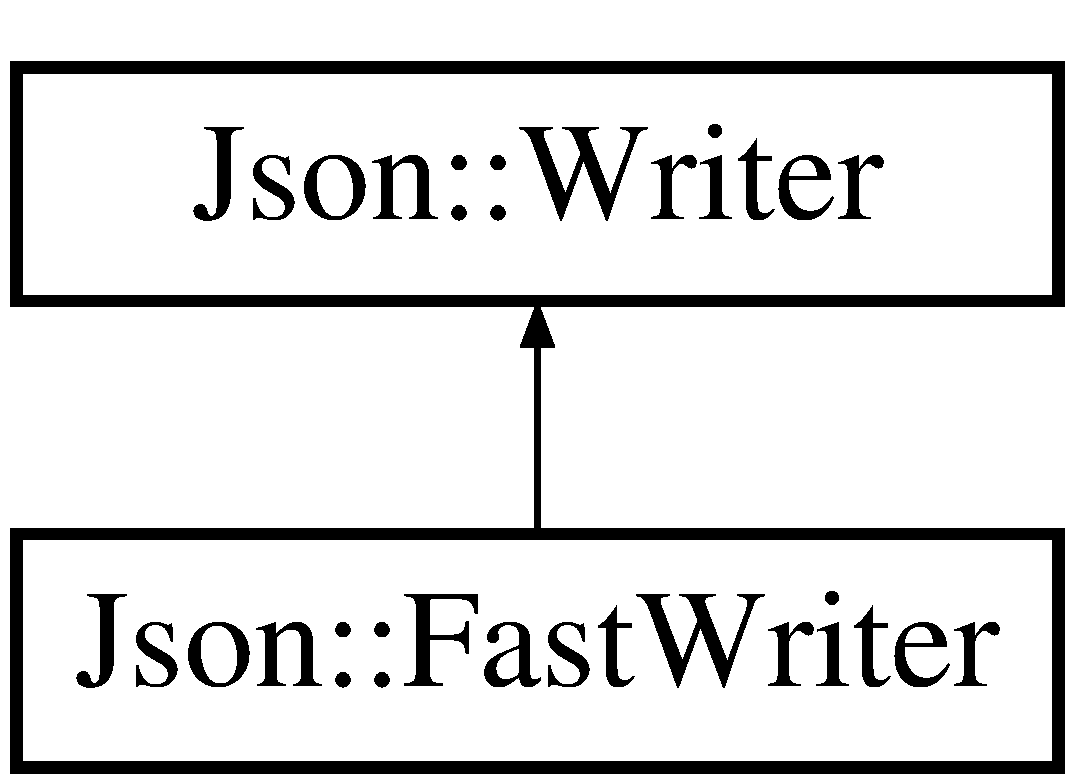
\includegraphics[height=2.000000cm]{class_json_1_1_fast_writer}
\end{center}
\end{figure}
\subsection*{Public Member Functions}
\begin{DoxyCompactItemize}
\item 
\hyperlink{class_json_1_1_fast_writer_a1bbc73ce1a1cc7b09cd1e02db3905170}{Fast\-Writer} ()
\item 
virtual \hyperlink{class_json_1_1_fast_writer_a7eb61405d041a915e5e980be97a707aa}{$\sim$\-Fast\-Writer} ()
\item 
void \hyperlink{class_json_1_1_fast_writer_a78d98e9f76d33660ad6e6a1abe287d45}{enable\-Y\-A\-M\-L\-Compatibility} ()
\item 
void \hyperlink{class_json_1_1_fast_writer_a6e93d8dce951e408517311026a065b40}{drop\-Null\-Placeholders} ()
\begin{DoxyCompactList}\small\item\em Drop the \char`\"{}null\char`\"{} string from the writer's output for null\-Values. Strictly speaking, this is not valid J\-S\-O\-N. But when the output is being fed to a browser's Javascript, it makes for smaller output and the browser can handle the output just fine. \end{DoxyCompactList}\item 
void \hyperlink{class_json_1_1_fast_writer_af4ee077d365d75941fb2688d97207a55}{omit\-Ending\-Line\-Feed} ()
\item 
virtual std\-::string \hyperlink{class_json_1_1_fast_writer_aa66218a56447222f91d64db618935a19}{write} (const \hyperlink{class_json_1_1_value}{Value} \&root)
\end{DoxyCompactItemize}


\subsection{Detailed Description}
Outputs a \hyperlink{class_json_1_1_value}{Value} in \href{http://www.json.org}{\tt J\-S\-O\-N} format without formatting (not human friendly). 

The J\-S\-O\-N document is written in a single line. It is not intended for 'human' consumption, but may be usefull to support feature such as R\-P\-C where bandwith is limited. \begin{DoxySeeAlso}{See Also}
\hyperlink{class_json_1_1_reader}{Reader}, \hyperlink{class_json_1_1_value}{Value} 
\end{DoxySeeAlso}


Definition at line 1801 of file json.\-hpp.



\subsection{Constructor \& Destructor Documentation}
\hypertarget{class_json_1_1_fast_writer_a1bbc73ce1a1cc7b09cd1e02db3905170}{\index{Json\-::\-Fast\-Writer@{Json\-::\-Fast\-Writer}!Fast\-Writer@{Fast\-Writer}}
\index{Fast\-Writer@{Fast\-Writer}!Json::FastWriter@{Json\-::\-Fast\-Writer}}
\subsubsection[{Fast\-Writer}]{\setlength{\rightskip}{0pt plus 5cm}Json\-::\-Fast\-Writer\-::\-Fast\-Writer (
\begin{DoxyParamCaption}
{}
\end{DoxyParamCaption}
)}}\label{class_json_1_1_fast_writer_a1bbc73ce1a1cc7b09cd1e02db3905170}


Definition at line 3144 of file json.\-cpp.

\hypertarget{class_json_1_1_fast_writer_a7eb61405d041a915e5e980be97a707aa}{\index{Json\-::\-Fast\-Writer@{Json\-::\-Fast\-Writer}!$\sim$\-Fast\-Writer@{$\sim$\-Fast\-Writer}}
\index{$\sim$\-Fast\-Writer@{$\sim$\-Fast\-Writer}!Json::FastWriter@{Json\-::\-Fast\-Writer}}
\subsubsection[{$\sim$\-Fast\-Writer}]{\setlength{\rightskip}{0pt plus 5cm}virtual Json\-::\-Fast\-Writer\-::$\sim$\-Fast\-Writer (
\begin{DoxyParamCaption}
{}
\end{DoxyParamCaption}
)\hspace{0.3cm}{\ttfamily [inline]}, {\ttfamily [virtual]}}}\label{class_json_1_1_fast_writer_a7eb61405d041a915e5e980be97a707aa}


Definition at line 1804 of file json.\-hpp.



\subsection{Member Function Documentation}
\hypertarget{class_json_1_1_fast_writer_a6e93d8dce951e408517311026a065b40}{\index{Json\-::\-Fast\-Writer@{Json\-::\-Fast\-Writer}!drop\-Null\-Placeholders@{drop\-Null\-Placeholders}}
\index{drop\-Null\-Placeholders@{drop\-Null\-Placeholders}!Json::FastWriter@{Json\-::\-Fast\-Writer}}
\subsubsection[{drop\-Null\-Placeholders}]{\setlength{\rightskip}{0pt plus 5cm}void Json\-::\-Fast\-Writer\-::drop\-Null\-Placeholders (
\begin{DoxyParamCaption}
{}
\end{DoxyParamCaption}
)}}\label{class_json_1_1_fast_writer_a6e93d8dce951e408517311026a065b40}


Drop the \char`\"{}null\char`\"{} string from the writer's output for null\-Values. Strictly speaking, this is not valid J\-S\-O\-N. But when the output is being fed to a browser's Javascript, it makes for smaller output and the browser can handle the output just fine. 



Definition at line 3150 of file json.\-cpp.

\hypertarget{class_json_1_1_fast_writer_a78d98e9f76d33660ad6e6a1abe287d45}{\index{Json\-::\-Fast\-Writer@{Json\-::\-Fast\-Writer}!enable\-Y\-A\-M\-L\-Compatibility@{enable\-Y\-A\-M\-L\-Compatibility}}
\index{enable\-Y\-A\-M\-L\-Compatibility@{enable\-Y\-A\-M\-L\-Compatibility}!Json::FastWriter@{Json\-::\-Fast\-Writer}}
\subsubsection[{enable\-Y\-A\-M\-L\-Compatibility}]{\setlength{\rightskip}{0pt plus 5cm}void Json\-::\-Fast\-Writer\-::enable\-Y\-A\-M\-L\-Compatibility (
\begin{DoxyParamCaption}
{}
\end{DoxyParamCaption}
)}}\label{class_json_1_1_fast_writer_a78d98e9f76d33660ad6e6a1abe287d45}


Definition at line 3148 of file json.\-cpp.

\hypertarget{class_json_1_1_fast_writer_af4ee077d365d75941fb2688d97207a55}{\index{Json\-::\-Fast\-Writer@{Json\-::\-Fast\-Writer}!omit\-Ending\-Line\-Feed@{omit\-Ending\-Line\-Feed}}
\index{omit\-Ending\-Line\-Feed@{omit\-Ending\-Line\-Feed}!Json::FastWriter@{Json\-::\-Fast\-Writer}}
\subsubsection[{omit\-Ending\-Line\-Feed}]{\setlength{\rightskip}{0pt plus 5cm}void Json\-::\-Fast\-Writer\-::omit\-Ending\-Line\-Feed (
\begin{DoxyParamCaption}
{}
\end{DoxyParamCaption}
)}}\label{class_json_1_1_fast_writer_af4ee077d365d75941fb2688d97207a55}


Definition at line 3152 of file json.\-cpp.

\hypertarget{class_json_1_1_fast_writer_aa66218a56447222f91d64db618935a19}{\index{Json\-::\-Fast\-Writer@{Json\-::\-Fast\-Writer}!write@{write}}
\index{write@{write}!Json::FastWriter@{Json\-::\-Fast\-Writer}}
\subsubsection[{write}]{\setlength{\rightskip}{0pt plus 5cm}std\-::string Json\-::\-Fast\-Writer\-::write (
\begin{DoxyParamCaption}
\item[{const {\bf Value} \&}]{root}
\end{DoxyParamCaption}
)\hspace{0.3cm}{\ttfamily [virtual]}}}\label{class_json_1_1_fast_writer_aa66218a56447222f91d64db618935a19}


Implements \hyperlink{class_json_1_1_writer_a7b2273a4ffd6f32b369ac8a53b7b5a0d}{Json\-::\-Writer}.



Definition at line 3154 of file json.\-cpp.



The documentation for this class was generated from the following files\-:\begin{DoxyCompactItemize}
\item 
/home/fushigisama/\-Documents/amon/includes/util/json/\hyperlink{json_8hpp}{json.\-hpp}\item 
/home/fushigisama/\-Documents/amon/src/util/json/\hyperlink{json_8cpp}{json.\-cpp}\end{DoxyCompactItemize}

\hypertarget{class_json_1_1_features}{\section{Json\-:\-:Features Class Reference}
\label{class_json_1_1_features}\index{Json\-::\-Features@{Json\-::\-Features}}
}


Configuration passed to reader and writer. This configuration object can be used to force the \hyperlink{class_json_1_1_reader}{Reader} or \hyperlink{class_json_1_1_writer}{Writer} to behave in a standard conforming way.  




{\ttfamily \#include $<$json.\-hpp$>$}

\subsection*{Public Member Functions}
\begin{DoxyCompactItemize}
\item 
\hyperlink{class_json_1_1_features_ad15a091cb61bb31323299a95970d2644}{Features} ()
\begin{DoxyCompactList}\small\item\em Initialize the configuration like Json\-Config\-::all\-Features;. \end{DoxyCompactList}\end{DoxyCompactItemize}
\subsection*{Static Public Member Functions}
\begin{DoxyCompactItemize}
\item 
static \hyperlink{class_json_1_1_features}{Features} \hyperlink{class_json_1_1_features_a63894da6e2c100b38741fa933f3d33ae}{all} ()
\begin{DoxyCompactList}\small\item\em A configuration that allows all features and assumes all strings are U\-T\-F-\/8. \end{DoxyCompactList}\item 
static \hyperlink{class_json_1_1_features}{Features} \hyperlink{class_json_1_1_features_ae23176c14b2e79e81fb61fb1a8ab58ee}{strict\-Mode} ()
\begin{DoxyCompactList}\small\item\em A configuration that is strictly compatible with the J\-S\-O\-N specification. \end{DoxyCompactList}\end{DoxyCompactItemize}
\subsection*{Public Attributes}
\begin{DoxyCompactItemize}
\item 
bool \hyperlink{class_json_1_1_features_a33afd389719624b6bdb23950b3c346c9}{allow\-Comments\-\_\-}
\begin{DoxyCompactList}\small\item\em {\ttfamily true} if comments are allowed. Default\-: {\ttfamily true}. \end{DoxyCompactList}\item 
bool \hyperlink{class_json_1_1_features_a1162c37a1458adc32582b585b552f9c3}{strict\-Root\-\_\-}
\item 
bool \hyperlink{class_json_1_1_features_a5076aa72c05c7596ac339ede36c97a6a}{allow\-Dropped\-Null\-Placeholders\-\_\-}
\begin{DoxyCompactList}\small\item\em {\ttfamily true} if dropped null placeholders are allowed. Default\-: {\ttfamily false}. \end{DoxyCompactList}\item 
bool \hyperlink{class_json_1_1_features_aff3cb16b79d15d3d761b11a0dd6d4d6b}{allow\-Numeric\-Keys\-\_\-}
\begin{DoxyCompactList}\small\item\em {\ttfamily true} if numeric object key are allowed. Default\-: {\ttfamily false}. \end{DoxyCompactList}\end{DoxyCompactItemize}


\subsection{Detailed Description}
Configuration passed to reader and writer. This configuration object can be used to force the \hyperlink{class_json_1_1_reader}{Reader} or \hyperlink{class_json_1_1_writer}{Writer} to behave in a standard conforming way. 

Definition at line 314 of file json.\-hpp.



\subsection{Constructor \& Destructor Documentation}
\hypertarget{class_json_1_1_features_ad15a091cb61bb31323299a95970d2644}{\index{Json\-::\-Features@{Json\-::\-Features}!Features@{Features}}
\index{Features@{Features}!Json::Features@{Json\-::\-Features}}
\subsubsection[{Features}]{\setlength{\rightskip}{0pt plus 5cm}Json\-::\-Features\-::\-Features (
\begin{DoxyParamCaption}
{}
\end{DoxyParamCaption}
)}}\label{class_json_1_1_features_ad15a091cb61bb31323299a95970d2644}


Initialize the configuration like Json\-Config\-::all\-Features;. 



Definition at line 215 of file json.\-cpp.



\subsection{Member Function Documentation}
\hypertarget{class_json_1_1_features_a63894da6e2c100b38741fa933f3d33ae}{\index{Json\-::\-Features@{Json\-::\-Features}!all@{all}}
\index{all@{all}!Json::Features@{Json\-::\-Features}}
\subsubsection[{all}]{\setlength{\rightskip}{0pt plus 5cm}{\bf Features} Json\-::\-Features\-::all (
\begin{DoxyParamCaption}
{}
\end{DoxyParamCaption}
)\hspace{0.3cm}{\ttfamily [static]}}}\label{class_json_1_1_features_a63894da6e2c100b38741fa933f3d33ae}


A configuration that allows all features and assumes all strings are U\-T\-F-\/8. 


\begin{DoxyItemize}
\item C \& C++ comments are allowed
\item Root object can be any J\-S\-O\-N value
\item Assumes \hyperlink{class_json_1_1_value}{Value} strings are encoded in U\-T\-F-\/8 
\end{DoxyItemize}

Definition at line 219 of file json.\-cpp.

\hypertarget{class_json_1_1_features_ae23176c14b2e79e81fb61fb1a8ab58ee}{\index{Json\-::\-Features@{Json\-::\-Features}!strict\-Mode@{strict\-Mode}}
\index{strict\-Mode@{strict\-Mode}!Json::Features@{Json\-::\-Features}}
\subsubsection[{strict\-Mode}]{\setlength{\rightskip}{0pt plus 5cm}{\bf Features} Json\-::\-Features\-::strict\-Mode (
\begin{DoxyParamCaption}
{}
\end{DoxyParamCaption}
)\hspace{0.3cm}{\ttfamily [static]}}}\label{class_json_1_1_features_ae23176c14b2e79e81fb61fb1a8ab58ee}


A configuration that is strictly compatible with the J\-S\-O\-N specification. 


\begin{DoxyItemize}
\item Comments are forbidden.
\item Root object must be either an array or an object value.
\item Assumes \hyperlink{class_json_1_1_value}{Value} strings are encoded in U\-T\-F-\/8 
\end{DoxyItemize}

Definition at line 221 of file json.\-cpp.



\subsection{Member Data Documentation}
\hypertarget{class_json_1_1_features_a33afd389719624b6bdb23950b3c346c9}{\index{Json\-::\-Features@{Json\-::\-Features}!allow\-Comments\-\_\-@{allow\-Comments\-\_\-}}
\index{allow\-Comments\-\_\-@{allow\-Comments\-\_\-}!Json::Features@{Json\-::\-Features}}
\subsubsection[{allow\-Comments\-\_\-}]{\setlength{\rightskip}{0pt plus 5cm}bool Json\-::\-Features\-::allow\-Comments\-\_\-}}\label{class_json_1_1_features_a33afd389719624b6bdb23950b3c346c9}


{\ttfamily true} if comments are allowed. Default\-: {\ttfamily true}. 



Definition at line 337 of file json.\-hpp.

\hypertarget{class_json_1_1_features_a5076aa72c05c7596ac339ede36c97a6a}{\index{Json\-::\-Features@{Json\-::\-Features}!allow\-Dropped\-Null\-Placeholders\-\_\-@{allow\-Dropped\-Null\-Placeholders\-\_\-}}
\index{allow\-Dropped\-Null\-Placeholders\-\_\-@{allow\-Dropped\-Null\-Placeholders\-\_\-}!Json::Features@{Json\-::\-Features}}
\subsubsection[{allow\-Dropped\-Null\-Placeholders\-\_\-}]{\setlength{\rightskip}{0pt plus 5cm}bool Json\-::\-Features\-::allow\-Dropped\-Null\-Placeholders\-\_\-}}\label{class_json_1_1_features_a5076aa72c05c7596ac339ede36c97a6a}


{\ttfamily true} if dropped null placeholders are allowed. Default\-: {\ttfamily false}. 



Definition at line 344 of file json.\-hpp.

\hypertarget{class_json_1_1_features_aff3cb16b79d15d3d761b11a0dd6d4d6b}{\index{Json\-::\-Features@{Json\-::\-Features}!allow\-Numeric\-Keys\-\_\-@{allow\-Numeric\-Keys\-\_\-}}
\index{allow\-Numeric\-Keys\-\_\-@{allow\-Numeric\-Keys\-\_\-}!Json::Features@{Json\-::\-Features}}
\subsubsection[{allow\-Numeric\-Keys\-\_\-}]{\setlength{\rightskip}{0pt plus 5cm}bool Json\-::\-Features\-::allow\-Numeric\-Keys\-\_\-}}\label{class_json_1_1_features_aff3cb16b79d15d3d761b11a0dd6d4d6b}


{\ttfamily true} if numeric object key are allowed. Default\-: {\ttfamily false}. 



Definition at line 347 of file json.\-hpp.

\hypertarget{class_json_1_1_features_a1162c37a1458adc32582b585b552f9c3}{\index{Json\-::\-Features@{Json\-::\-Features}!strict\-Root\-\_\-@{strict\-Root\-\_\-}}
\index{strict\-Root\-\_\-@{strict\-Root\-\_\-}!Json::Features@{Json\-::\-Features}}
\subsubsection[{strict\-Root\-\_\-}]{\setlength{\rightskip}{0pt plus 5cm}bool Json\-::\-Features\-::strict\-Root\-\_\-}}\label{class_json_1_1_features_a1162c37a1458adc32582b585b552f9c3}
{\ttfamily true} if root must be either an array or an object value. Default\-: {\ttfamily false}. 

Definition at line 341 of file json.\-hpp.



The documentation for this class was generated from the following files\-:\begin{DoxyCompactItemize}
\item 
/home/fushigisama/\-Documents/amon/includes/util/json/\hyperlink{json_8hpp}{json.\-hpp}\item 
/home/fushigisama/\-Documents/amon/src/util/json/\hyperlink{json_8cpp}{json.\-cpp}\end{DoxyCompactItemize}

\hypertarget{classamon_1_1_fenwick_tree}{\section{amon\-:\-:Fenwick\-Tree Class Reference}
\label{classamon_1_1_fenwick_tree}\index{amon\-::\-Fenwick\-Tree@{amon\-::\-Fenwick\-Tree}}
}


{\ttfamily \#include $<$fenwick.\-hpp$>$}

\subsection*{Public Member Functions}
\begin{DoxyCompactItemize}
\item 
\hyperlink{classamon_1_1_fenwick_tree_ad26fda62f83c3e8945d7fa1671e72197}{Fenwick\-Tree} (int n)
\item 
\hyperlink{classamon_1_1_fenwick_tree_a9e05cac381dc28d7d3dbfcaa66844e68}{$\sim$\-Fenwick\-Tree} ()
\item 
void \hyperlink{classamon_1_1_fenwick_tree_a690ed7f993820c730a04482bb9c330d7}{add} (int x, int v)
\item 
int \hyperlink{classamon_1_1_fenwick_tree_ac44569034b5bac7d16fa3ec48dfbd770}{query} (int x)
\end{DoxyCompactItemize}


\subsection{Detailed Description}
Simple implementation of the Fenwick Tree. O(\-N) space needed!! Operations\-: add(x, v)\-: adds x to position v (log\-N) query(x)\-: query sum of elements up to x (log\-N) 

Definition at line 13 of file fenwick.\-hpp.



\subsection{Constructor \& Destructor Documentation}
\hypertarget{classamon_1_1_fenwick_tree_ad26fda62f83c3e8945d7fa1671e72197}{\index{amon\-::\-Fenwick\-Tree@{amon\-::\-Fenwick\-Tree}!Fenwick\-Tree@{Fenwick\-Tree}}
\index{Fenwick\-Tree@{Fenwick\-Tree}!amon::FenwickTree@{amon\-::\-Fenwick\-Tree}}
\subsubsection[{Fenwick\-Tree}]{\setlength{\rightskip}{0pt plus 5cm}amon\-::\-Fenwick\-Tree\-::\-Fenwick\-Tree (
\begin{DoxyParamCaption}
\item[{int}]{n}
\end{DoxyParamCaption}
)}}\label{classamon_1_1_fenwick_tree_ad26fda62f83c3e8945d7fa1671e72197}
Constructor 
\begin{DoxyParams}{Parameters}
{\em n} & Number of elements. \\
\hline
\end{DoxyParams}


Definition at line 4 of file fenwick.\-cpp.

\hypertarget{classamon_1_1_fenwick_tree_a9e05cac381dc28d7d3dbfcaa66844e68}{\index{amon\-::\-Fenwick\-Tree@{amon\-::\-Fenwick\-Tree}!$\sim$\-Fenwick\-Tree@{$\sim$\-Fenwick\-Tree}}
\index{$\sim$\-Fenwick\-Tree@{$\sim$\-Fenwick\-Tree}!amon::FenwickTree@{amon\-::\-Fenwick\-Tree}}
\subsubsection[{$\sim$\-Fenwick\-Tree}]{\setlength{\rightskip}{0pt plus 5cm}amon\-::\-Fenwick\-Tree\-::$\sim$\-Fenwick\-Tree (
\begin{DoxyParamCaption}
{}
\end{DoxyParamCaption}
)}}\label{classamon_1_1_fenwick_tree_a9e05cac381dc28d7d3dbfcaa66844e68}


Definition at line 9 of file fenwick.\-cpp.



\subsection{Member Function Documentation}
\hypertarget{classamon_1_1_fenwick_tree_a690ed7f993820c730a04482bb9c330d7}{\index{amon\-::\-Fenwick\-Tree@{amon\-::\-Fenwick\-Tree}!add@{add}}
\index{add@{add}!amon::FenwickTree@{amon\-::\-Fenwick\-Tree}}
\subsubsection[{add}]{\setlength{\rightskip}{0pt plus 5cm}void amon\-::\-Fenwick\-Tree\-::add (
\begin{DoxyParamCaption}
\item[{int}]{x, }
\item[{int}]{v}
\end{DoxyParamCaption}
)}}\label{classamon_1_1_fenwick_tree_a690ed7f993820c730a04482bb9c330d7}
Adds v to position x in the tree. 
\begin{DoxyParams}{Parameters}
{\em x} & The position to increment \\
\hline
{\em v} & The value to increment \\
\hline
\end{DoxyParams}


Definition at line 11 of file fenwick.\-cpp.

\hypertarget{classamon_1_1_fenwick_tree_ac44569034b5bac7d16fa3ec48dfbd770}{\index{amon\-::\-Fenwick\-Tree@{amon\-::\-Fenwick\-Tree}!query@{query}}
\index{query@{query}!amon::FenwickTree@{amon\-::\-Fenwick\-Tree}}
\subsubsection[{query}]{\setlength{\rightskip}{0pt plus 5cm}int amon\-::\-Fenwick\-Tree\-::query (
\begin{DoxyParamCaption}
\item[{int}]{x}
\end{DoxyParamCaption}
)}}\label{classamon_1_1_fenwick_tree_ac44569034b5bac7d16fa3ec48dfbd770}
Queries sum of all positions up to x. 
\begin{DoxyParams}{Parameters}
{\em x} & The position to query up to. \\
\hline
\end{DoxyParams}
\begin{DoxyReturn}{Returns}
The value sought. 
\end{DoxyReturn}


Definition at line 18 of file fenwick.\-cpp.



The documentation for this class was generated from the following files\-:\begin{DoxyCompactItemize}
\item 
/home/fushigisama/\-Documents/amon/includes/util/\hyperlink{fenwick_8hpp}{fenwick.\-hpp}\item 
/home/fushigisama/\-Documents/amon/src/util/\hyperlink{fenwick_8cpp}{fenwick.\-cpp}\end{DoxyCompactItemize}

\hypertarget{classamon_1_1_graph}{\section{amon\-:\-:Graph Class Reference}
\label{classamon_1_1_graph}\index{amon\-::\-Graph@{amon\-::\-Graph}}
}


{\ttfamily \#include $<$graph.\-hpp$>$}

\subsection*{Public Member Functions}
\begin{DoxyCompactItemize}
\item 
\hyperlink{classamon_1_1_graph_a8dbd046ce57a0c624c7abe573b174ce1}{Graph} ()
\item 
\hyperlink{classamon_1_1_graph_a40dd78be5732f86fa3df8d687d0e5728}{Graph} (int n)
\item 
int \hyperlink{classamon_1_1_graph_a7c7ef2759921bb87aa8c69c28ea62f8f}{nodes\-Qty} () const 
\item 
int \hyperlink{classamon_1_1_graph_a705be004387c64a5ce5aa668b0c4e9d7}{edges\-Qty} () const 
\item 
int \hyperlink{classamon_1_1_graph_aa7f39dcf5b2fab62d0b9399bc759ff27}{add\-Node} ()
\item 
void \hyperlink{classamon_1_1_graph_af3a842a93c90db66a7f301c685e51b3a}{remove\-Node} (int index)
\item 
void \hyperlink{classamon_1_1_graph_a02016704b31a4bf3a277fb4fcb8c1d72}{add\-Directed\-Edge} (int A, int B, double w)
\item 
void \hyperlink{classamon_1_1_graph_a98b71efc14d469813b8d1c679ca22fa3}{add\-Undirected\-Edge} (int A, int B, double w)
\item 
int \hyperlink{classamon_1_1_graph_a2500d2f93404a3ce691396db4ca0ea92}{out\-Degree} (int x)
\begin{DoxyCompactList}\small\item\em \{ Returns the out\-Degree of node x. \} \end{DoxyCompactList}\item 
double \hyperlink{classamon_1_1_graph_ac97e95d56f333fa63755458cc9443cc6}{mean\-Degree} ()
\item 
double \hyperlink{classamon_1_1_graph_a6e9098ead3849a382e3a5d1949599947}{global\-Clustering\-Coefficient} ()
\item 
std\-::list$<$ std\-::pair$<$ int, \\*
double $>$ $>$\-::iterator \hyperlink{classamon_1_1_graph_a182d3611b27058fda589269589b62b41}{neighboors\-Begin} (int node)
\item 
std\-::list$<$ std\-::pair$<$ int, \\*
double $>$ $>$\-::iterator \hyperlink{classamon_1_1_graph_acaeb02df5f8d9bd71cf4aae11e89532f}{neighboors\-End} (int node)
\item 
int \hyperlink{classamon_1_1_graph_a0ea3919c713485cfc5b24fe3ef1aaf24}{bridges} ()
\item 
double \hyperlink{classamon_1_1_graph_a31712319c837723444fc5f83a272b41d}{mean\-Degree} (double P)
\item 
double \hyperlink{classamon_1_1_graph_ac0e052c99a3842aa205480156217c52b}{average\-Distance} ()
\item 
std\-::unordered\-\_\-map$<$ int, int $>$ \hyperlink{classamon_1_1_graph_a658ec90c39eb57958a286574cf463224}{bfs} (int src)
\item 
void \hyperlink{classamon_1_1_graph_a88ee59e7d320f210c4bb9eb1e4eff476}{next\-Neighboor} (std\-::list$<$ std\-::pair$<$ int, double $>$ $>$\-::iterator \&iterator, int node)
\item 
bool \hyperlink{classamon_1_1_graph_a17d2727539c869cb0a047d81b0236dad}{is\-Deleted} (int index)
\item 
std\-::string \hyperlink{classamon_1_1_graph_ad18818eecab5f005c6c3a12ca2461c52}{to\-Dot} (bool is\-Directed)
\begin{DoxyCompactList}\small\item\em \{ Returns a .dot description of the graph. \} \end{DoxyCompactList}\item 
std\-::string \hyperlink{classamon_1_1_graph_ad2c36a69520088dd76da23e13b372464}{to\-Dot} (bool is\-Directed, std\-::vector$<$ bool $>$ inc)
\begin{DoxyCompactList}\small\item\em \{ Returns a .dot description of the graph. \} \end{DoxyCompactList}\end{DoxyCompactItemize}
\subsection*{Static Public Attributes}
\begin{DoxyCompactItemize}
\item 
static const double \hyperlink{classamon_1_1_graph_a1bddebc6360d5154a86dbd75856b6a6c}{E\-P\-S} = 1e-\/7
\end{DoxyCompactItemize}


\subsection{Detailed Description}


Definition at line 14 of file graph.\-hpp.



\subsection{Constructor \& Destructor Documentation}
\hypertarget{classamon_1_1_graph_a8dbd046ce57a0c624c7abe573b174ce1}{\index{amon\-::\-Graph@{amon\-::\-Graph}!Graph@{Graph}}
\index{Graph@{Graph}!amon::Graph@{amon\-::\-Graph}}
\subsubsection[{Graph}]{\setlength{\rightskip}{0pt plus 5cm}amon\-::\-Graph\-::\-Graph (
\begin{DoxyParamCaption}
{}
\end{DoxyParamCaption}
)}}\label{classamon_1_1_graph_a8dbd046ce57a0c624c7abe573b174ce1}
Empty Constructor 

Definition at line 11 of file graph.\-cpp.

\hypertarget{classamon_1_1_graph_a40dd78be5732f86fa3df8d687d0e5728}{\index{amon\-::\-Graph@{amon\-::\-Graph}!Graph@{Graph}}
\index{Graph@{Graph}!amon::Graph@{amon\-::\-Graph}}
\subsubsection[{Graph}]{\setlength{\rightskip}{0pt plus 5cm}amon\-::\-Graph\-::\-Graph (
\begin{DoxyParamCaption}
\item[{int}]{n}
\end{DoxyParamCaption}
)}}\label{classamon_1_1_graph_a40dd78be5732f86fa3df8d687d0e5728}
Creates a graph with n nodes 
\begin{DoxyParams}{Parameters}
{\em n} & The number of initial nodes in the graph \\
\hline
\end{DoxyParams}


Definition at line 17 of file graph.\-cpp.



\subsection{Member Function Documentation}
\hypertarget{classamon_1_1_graph_a02016704b31a4bf3a277fb4fcb8c1d72}{\index{amon\-::\-Graph@{amon\-::\-Graph}!add\-Directed\-Edge@{add\-Directed\-Edge}}
\index{add\-Directed\-Edge@{add\-Directed\-Edge}!amon::Graph@{amon\-::\-Graph}}
\subsubsection[{add\-Directed\-Edge}]{\setlength{\rightskip}{0pt plus 5cm}void amon\-::\-Graph\-::add\-Directed\-Edge (
\begin{DoxyParamCaption}
\item[{int}]{A, }
\item[{int}]{B, }
\item[{double}]{w}
\end{DoxyParamCaption}
)}}\label{classamon_1_1_graph_a02016704b31a4bf3a277fb4fcb8c1d72}
Adds a directed edge between vertices A and B with weight w. 
\begin{DoxyParams}{Parameters}
{\em A} & The source of the edge \\
\hline
{\em B} & The destination of the edge \\
\hline
{\em w} & The weight of the edge \\
\hline
\end{DoxyParams}


Definition at line 56 of file graph.\-cpp.

\hypertarget{classamon_1_1_graph_aa7f39dcf5b2fab62d0b9399bc759ff27}{\index{amon\-::\-Graph@{amon\-::\-Graph}!add\-Node@{add\-Node}}
\index{add\-Node@{add\-Node}!amon::Graph@{amon\-::\-Graph}}
\subsubsection[{add\-Node}]{\setlength{\rightskip}{0pt plus 5cm}int amon\-::\-Graph\-::add\-Node (
\begin{DoxyParamCaption}
{}
\end{DoxyParamCaption}
)}}\label{classamon_1_1_graph_aa7f39dcf5b2fab62d0b9399bc759ff27}
Adds a node to the graph. \begin{DoxyReturn}{Returns}
The index of the newly created node. 
\end{DoxyReturn}


Definition at line 33 of file graph.\-cpp.

\hypertarget{classamon_1_1_graph_a98b71efc14d469813b8d1c679ca22fa3}{\index{amon\-::\-Graph@{amon\-::\-Graph}!add\-Undirected\-Edge@{add\-Undirected\-Edge}}
\index{add\-Undirected\-Edge@{add\-Undirected\-Edge}!amon::Graph@{amon\-::\-Graph}}
\subsubsection[{add\-Undirected\-Edge}]{\setlength{\rightskip}{0pt plus 5cm}void amon\-::\-Graph\-::add\-Undirected\-Edge (
\begin{DoxyParamCaption}
\item[{int}]{A, }
\item[{int}]{B, }
\item[{double}]{w}
\end{DoxyParamCaption}
)}}\label{classamon_1_1_graph_a98b71efc14d469813b8d1c679ca22fa3}
Adds an undirected edge between vertices A and B with weight w. 
\begin{DoxyParams}{Parameters}
{\em A} & One of the end-\/points of the edge \\
\hline
{\em B} & The other endpoint \\
\hline
{\em w} & The weight of the edge \\
\hline
\end{DoxyParams}


Definition at line 63 of file graph.\-cpp.

\hypertarget{classamon_1_1_graph_ac0e052c99a3842aa205480156217c52b}{\index{amon\-::\-Graph@{amon\-::\-Graph}!average\-Distance@{average\-Distance}}
\index{average\-Distance@{average\-Distance}!amon::Graph@{amon\-::\-Graph}}
\subsubsection[{average\-Distance}]{\setlength{\rightskip}{0pt plus 5cm}double amon\-::\-Graph\-::average\-Distance (
\begin{DoxyParamCaption}
{}
\end{DoxyParamCaption}
)}}\label{classamon_1_1_graph_ac0e052c99a3842aa205480156217c52b}
Calculates the average distance on the graph. Not using weights. \begin{DoxyReturn}{Returns}
The average distance excluding non-\/connected pairs. 
\end{DoxyReturn}
\hypertarget{classamon_1_1_graph_a658ec90c39eb57958a286574cf463224}{\index{amon\-::\-Graph@{amon\-::\-Graph}!bfs@{bfs}}
\index{bfs@{bfs}!amon::Graph@{amon\-::\-Graph}}
\subsubsection[{bfs}]{\setlength{\rightskip}{0pt plus 5cm}std\-::unordered\-\_\-map$<$ int, int $>$ amon\-::\-Graph\-::bfs (
\begin{DoxyParamCaption}
\item[{int}]{src}
\end{DoxyParamCaption}
)}}\label{classamon_1_1_graph_a658ec90c39eb57958a286574cf463224}
Breadth-\/\-First search to find minimum paths. 
\begin{DoxyParams}{Parameters}
{\em src} & The source node. \\
\hline
\end{DoxyParams}
\begin{DoxyReturn}{Returns}
An unordered\-\_\-map containing the distances to nodes rechable from the source. 
\end{DoxyReturn}


Definition at line 205 of file graph.\-cpp.

\hypertarget{classamon_1_1_graph_a0ea3919c713485cfc5b24fe3ef1aaf24}{\index{amon\-::\-Graph@{amon\-::\-Graph}!bridges@{bridges}}
\index{bridges@{bridges}!amon::Graph@{amon\-::\-Graph}}
\subsubsection[{bridges}]{\setlength{\rightskip}{0pt plus 5cm}int amon\-::\-Graph\-::bridges (
\begin{DoxyParamCaption}
{}
\end{DoxyParamCaption}
)}}\label{classamon_1_1_graph_a0ea3919c713485cfc5b24fe3ef1aaf24}
Count the number of bridges on the graph. \begin{DoxyReturn}{Returns}
Number of bridges 
\end{DoxyReturn}


Definition at line 177 of file graph.\-cpp.

\hypertarget{classamon_1_1_graph_a705be004387c64a5ce5aa668b0c4e9d7}{\index{amon\-::\-Graph@{amon\-::\-Graph}!edges\-Qty@{edges\-Qty}}
\index{edges\-Qty@{edges\-Qty}!amon::Graph@{amon\-::\-Graph}}
\subsubsection[{edges\-Qty}]{\setlength{\rightskip}{0pt plus 5cm}int amon\-::\-Graph\-::edges\-Qty (
\begin{DoxyParamCaption}
{}
\end{DoxyParamCaption}
) const}}\label{classamon_1_1_graph_a705be004387c64a5ce5aa668b0c4e9d7}
Returns the number of edges in the graph. \begin{DoxyReturn}{Returns}
The number of edges in the graph. 
\end{DoxyReturn}


Definition at line 29 of file graph.\-cpp.

\hypertarget{classamon_1_1_graph_a6e9098ead3849a382e3a5d1949599947}{\index{amon\-::\-Graph@{amon\-::\-Graph}!global\-Clustering\-Coefficient@{global\-Clustering\-Coefficient}}
\index{global\-Clustering\-Coefficient@{global\-Clustering\-Coefficient}!amon::Graph@{amon\-::\-Graph}}
\subsubsection[{global\-Clustering\-Coefficient}]{\setlength{\rightskip}{0pt plus 5cm}double amon\-::\-Graph\-::global\-Clustering\-Coefficient (
\begin{DoxyParamCaption}
{}
\end{DoxyParamCaption}
)}}\label{classamon_1_1_graph_a6e9098ead3849a382e3a5d1949599947}
The clustering coefficient of the graph \begin{DoxyReturn}{Returns}
The clustering coefficient of the graph 
\end{DoxyReturn}


Definition at line 115 of file graph.\-cpp.

\hypertarget{classamon_1_1_graph_a17d2727539c869cb0a047d81b0236dad}{\index{amon\-::\-Graph@{amon\-::\-Graph}!is\-Deleted@{is\-Deleted}}
\index{is\-Deleted@{is\-Deleted}!amon::Graph@{amon\-::\-Graph}}
\subsubsection[{is\-Deleted}]{\setlength{\rightskip}{0pt plus 5cm}bool amon\-::\-Graph\-::is\-Deleted (
\begin{DoxyParamCaption}
\item[{int}]{index}
\end{DoxyParamCaption}
)}}\label{classamon_1_1_graph_a17d2727539c869cb0a047d81b0236dad}
Tests if node is deleted 
\begin{DoxyParams}{Parameters}
{\em index} & Index of the node to test \\
\hline
\end{DoxyParams}
\begin{DoxyReturn}{Returns}
True if given node is deleted. 
\end{DoxyReturn}


Definition at line 222 of file graph.\-cpp.

\hypertarget{classamon_1_1_graph_ac97e95d56f333fa63755458cc9443cc6}{\index{amon\-::\-Graph@{amon\-::\-Graph}!mean\-Degree@{mean\-Degree}}
\index{mean\-Degree@{mean\-Degree}!amon::Graph@{amon\-::\-Graph}}
\subsubsection[{mean\-Degree}]{\setlength{\rightskip}{0pt plus 5cm}double amon\-::\-Graph\-::mean\-Degree (
\begin{DoxyParamCaption}
{}
\end{DoxyParamCaption}
)}}\label{classamon_1_1_graph_ac97e95d56f333fa63755458cc9443cc6}
Calculates the mean degree of the graph \begin{DoxyReturn}{Returns}
The mean degree of the graph 
\end{DoxyReturn}


Definition at line 111 of file graph.\-cpp.

\hypertarget{classamon_1_1_graph_a31712319c837723444fc5f83a272b41d}{\index{amon\-::\-Graph@{amon\-::\-Graph}!mean\-Degree@{mean\-Degree}}
\index{mean\-Degree@{mean\-Degree}!amon::Graph@{amon\-::\-Graph}}
\subsubsection[{mean\-Degree}]{\setlength{\rightskip}{0pt plus 5cm}double amon\-::\-Graph\-::mean\-Degree (
\begin{DoxyParamCaption}
\item[{double}]{P}
\end{DoxyParamCaption}
)}}\label{classamon_1_1_graph_a31712319c837723444fc5f83a272b41d}
Return the mean degree of the P percent nodes with highest degrees. 
\begin{DoxyParams}{Parameters}
{\em P} & The desired percentage \\
\hline
\end{DoxyParams}
\begin{DoxyReturn}{Returns}
The mean degree. 
\end{DoxyReturn}


Definition at line 189 of file graph.\-cpp.

\hypertarget{classamon_1_1_graph_a182d3611b27058fda589269589b62b41}{\index{amon\-::\-Graph@{amon\-::\-Graph}!neighboors\-Begin@{neighboors\-Begin}}
\index{neighboors\-Begin@{neighboors\-Begin}!amon::Graph@{amon\-::\-Graph}}
\subsubsection[{neighboors\-Begin}]{\setlength{\rightskip}{0pt plus 5cm}std\-::list$<$ std\-::pair$<$ int, double $>$ $>$\-::iterator amon\-::\-Graph\-::neighboors\-Begin (
\begin{DoxyParamCaption}
\item[{int}]{node}
\end{DoxyParamCaption}
)}}\label{classamon_1_1_graph_a182d3611b27058fda589269589b62b41}
Returns an iterator to the begining of the adjacency list of a node. 
\begin{DoxyParams}{Parameters}
{\em node} & The node to get neighboors from \\
\hline
\end{DoxyParams}
\begin{DoxyReturn}{Returns}
An iterator to the beggining of the node list. 
\end{DoxyReturn}


Definition at line 72 of file graph.\-cpp.

\hypertarget{classamon_1_1_graph_acaeb02df5f8d9bd71cf4aae11e89532f}{\index{amon\-::\-Graph@{amon\-::\-Graph}!neighboors\-End@{neighboors\-End}}
\index{neighboors\-End@{neighboors\-End}!amon::Graph@{amon\-::\-Graph}}
\subsubsection[{neighboors\-End}]{\setlength{\rightskip}{0pt plus 5cm}std\-::list$<$ std\-::pair$<$ int, double $>$ $>$\-::iterator amon\-::\-Graph\-::neighboors\-End (
\begin{DoxyParamCaption}
\item[{int}]{node}
\end{DoxyParamCaption}
)}}\label{classamon_1_1_graph_acaeb02df5f8d9bd71cf4aae11e89532f}
Returns a const\-\_\-iterator to the end of the adjacency list of node. 
\begin{DoxyParams}{Parameters}
{\em node} & The node to get the iterator from \\
\hline
\end{DoxyParams}


Definition at line 86 of file graph.\-cpp.

\hypertarget{classamon_1_1_graph_a88ee59e7d320f210c4bb9eb1e4eff476}{\index{amon\-::\-Graph@{amon\-::\-Graph}!next\-Neighboor@{next\-Neighboor}}
\index{next\-Neighboor@{next\-Neighboor}!amon::Graph@{amon\-::\-Graph}}
\subsubsection[{next\-Neighboor}]{\setlength{\rightskip}{0pt plus 5cm}void amon\-::\-Graph\-::next\-Neighboor (
\begin{DoxyParamCaption}
\item[{std\-::list$<$ std\-::pair$<$ int, double $>$ $>$\-::iterator \&}]{iterator, }
\item[{int}]{node}
\end{DoxyParamCaption}
)}}\label{classamon_1_1_graph_a88ee59e7d320f210c4bb9eb1e4eff476}
Advances the adjacency list iterator to the next neighboor. 
\begin{DoxyParams}{Parameters}
{\em iterator} & The iterator to advance \\
\hline
{\em node} & The node related to the iterator \\
\hline
\end{DoxyParams}


Definition at line 94 of file graph.\-cpp.

\hypertarget{classamon_1_1_graph_a7c7ef2759921bb87aa8c69c28ea62f8f}{\index{amon\-::\-Graph@{amon\-::\-Graph}!nodes\-Qty@{nodes\-Qty}}
\index{nodes\-Qty@{nodes\-Qty}!amon::Graph@{amon\-::\-Graph}}
\subsubsection[{nodes\-Qty}]{\setlength{\rightskip}{0pt plus 5cm}int amon\-::\-Graph\-::nodes\-Qty (
\begin{DoxyParamCaption}
{}
\end{DoxyParamCaption}
) const}}\label{classamon_1_1_graph_a7c7ef2759921bb87aa8c69c28ea62f8f}
Returns the number of nodes in the graph. \begin{DoxyReturn}{Returns}
The number of nodes in the graph. 
\end{DoxyReturn}


Definition at line 25 of file graph.\-cpp.

\hypertarget{classamon_1_1_graph_a2500d2f93404a3ce691396db4ca0ea92}{\index{amon\-::\-Graph@{amon\-::\-Graph}!out\-Degree@{out\-Degree}}
\index{out\-Degree@{out\-Degree}!amon::Graph@{amon\-::\-Graph}}
\subsubsection[{out\-Degree}]{\setlength{\rightskip}{0pt plus 5cm}int amon\-::\-Graph\-::out\-Degree (
\begin{DoxyParamCaption}
\item[{int}]{x}
\end{DoxyParamCaption}
)}}\label{classamon_1_1_graph_a2500d2f93404a3ce691396db4ca0ea92}


\{ Returns the out\-Degree of node x. \} 


\begin{DoxyParams}[1]{Parameters}
\mbox{\tt in}  & {\em x} & \{ The index of the node. \}\\
\hline
\end{DoxyParams}
\begin{DoxyReturn}{Returns}
\{ The out\-Degree of the node. \} 
\end{DoxyReturn}


Definition at line 107 of file graph.\-cpp.

\hypertarget{classamon_1_1_graph_af3a842a93c90db66a7f301c685e51b3a}{\index{amon\-::\-Graph@{amon\-::\-Graph}!remove\-Node@{remove\-Node}}
\index{remove\-Node@{remove\-Node}!amon::Graph@{amon\-::\-Graph}}
\subsubsection[{remove\-Node}]{\setlength{\rightskip}{0pt plus 5cm}void amon\-::\-Graph\-::remove\-Node (
\begin{DoxyParamCaption}
\item[{int}]{index}
\end{DoxyParamCaption}
)}}\label{classamon_1_1_graph_af3a842a93c90db66a7f301c685e51b3a}
Removes a node from the graph/ 
\begin{DoxyParams}{Parameters}
{\em index} & Index of the node to be removed. If the node is not present nothing will happen. \\
\hline
\end{DoxyParams}


Definition at line 50 of file graph.\-cpp.

\hypertarget{classamon_1_1_graph_ad18818eecab5f005c6c3a12ca2461c52}{\index{amon\-::\-Graph@{amon\-::\-Graph}!to\-Dot@{to\-Dot}}
\index{to\-Dot@{to\-Dot}!amon::Graph@{amon\-::\-Graph}}
\subsubsection[{to\-Dot}]{\setlength{\rightskip}{0pt plus 5cm}std\-::string amon\-::\-Graph\-::to\-Dot (
\begin{DoxyParamCaption}
\item[{bool}]{is\-Directed}
\end{DoxyParamCaption}
)}}\label{classamon_1_1_graph_ad18818eecab5f005c6c3a12ca2461c52}


\{ Returns a .dot description of the graph. \} 


\begin{DoxyParams}{Parameters}
{\em is\-Directed} & True if graph is directed. \\
\hline
\end{DoxyParams}
\begin{DoxyReturn}{Returns}
\{ A std\-::string containing a .dot description of the graph \} 
\end{DoxyReturn}


Definition at line 227 of file graph.\-cpp.

\hypertarget{classamon_1_1_graph_ad2c36a69520088dd76da23e13b372464}{\index{amon\-::\-Graph@{amon\-::\-Graph}!to\-Dot@{to\-Dot}}
\index{to\-Dot@{to\-Dot}!amon::Graph@{amon\-::\-Graph}}
\subsubsection[{to\-Dot}]{\setlength{\rightskip}{0pt plus 5cm}std\-::string amon\-::\-Graph\-::to\-Dot (
\begin{DoxyParamCaption}
\item[{bool}]{is\-Directed, }
\item[{std\-::vector$<$ bool $>$}]{inc}
\end{DoxyParamCaption}
)}}\label{classamon_1_1_graph_ad2c36a69520088dd76da23e13b372464}


\{ Returns a .dot description of the graph. \} 


\begin{DoxyParams}[1]{Parameters}
\mbox{\tt in}  & {\em is\-Directed} & \{ True if graph is directed. \} \\
\hline
\mbox{\tt in}  & {\em inc} & \{ A vector of bools that is 1 in the i-\/th position if the i-\/th node should be included. \}\\
\hline
\end{DoxyParams}
\begin{DoxyReturn}{Returns}
\{ A std\-::string containing a .dot description of the graph \} 
\end{DoxyReturn}


Definition at line 243 of file graph.\-cpp.



\subsection{Member Data Documentation}
\hypertarget{classamon_1_1_graph_a1bddebc6360d5154a86dbd75856b6a6c}{\index{amon\-::\-Graph@{amon\-::\-Graph}!E\-P\-S@{E\-P\-S}}
\index{E\-P\-S@{E\-P\-S}!amon::Graph@{amon\-::\-Graph}}
\subsubsection[{E\-P\-S}]{\setlength{\rightskip}{0pt plus 5cm}const double amon\-::\-Graph\-::\-E\-P\-S = 1e-\/7\hspace{0.3cm}{\ttfamily [static]}}}\label{classamon_1_1_graph_a1bddebc6360d5154a86dbd75856b6a6c}


Definition at line 18 of file graph.\-hpp.



The documentation for this class was generated from the following files\-:\begin{DoxyCompactItemize}
\item 
includes/graph/\hyperlink{graph_8hpp}{graph.\-hpp}\item 
src/graph/\hyperlink{graph_8cpp}{graph.\-cpp}\end{DoxyCompactItemize}

\hypertarget{classamon_1_1_information_network}{\section{amon\-:\-:Information\-Network Class Reference}
\label{classamon_1_1_information_network}\index{amon\-::\-Information\-Network@{amon\-::\-Information\-Network}}
}


\{ Provides analysis on networks that represent information spread from people to people. \}  




{\ttfamily \#include $<$information\-\_\-spread.\-hpp$>$}

\subsection*{Public Member Functions}
\begin{DoxyCompactItemize}
\item 
\hyperlink{classamon_1_1_information_network_ac1ac48f7de78b78667fe432ea98f17b8}{Information\-Network} (\hyperlink{classamon_1_1_graph}{amon\-::\-Graph} g)
\begin{DoxyCompactList}\small\item\em \{ Constructor \} \end{DoxyCompactList}\item 
std\-::vector$<$ std\-::pair$<$ int, \\*
int $>$ $>$ \hyperlink{classamon_1_1_information_network_ae4b4110a07671dda3f0431d36a1d94a7}{information\-Depth} ()
\begin{DoxyCompactList}\small\item\em \{ Returns a series of pairs (r, d). \} \end{DoxyCompactList}\item 
std\-::vector$<$ double $>$ \hyperlink{classamon_1_1_information_network_ac134e23dd425ba9b2fdd3d4ab7206a7d}{loss\-Of\-Attention} ()
\begin{DoxyCompactList}\small\item\em \{ Returns the attention loss index for every vertex on the network. \} \end{DoxyCompactList}\end{DoxyCompactItemize}


\subsection{Detailed Description}
\{ Provides analysis on networks that represent information spread from people to people. \} 

Definition at line 12 of file information\-\_\-spread.\-hpp.



\subsection{Constructor \& Destructor Documentation}
\hypertarget{classamon_1_1_information_network_ac1ac48f7de78b78667fe432ea98f17b8}{\index{amon\-::\-Information\-Network@{amon\-::\-Information\-Network}!Information\-Network@{Information\-Network}}
\index{Information\-Network@{Information\-Network}!amon::InformationNetwork@{amon\-::\-Information\-Network}}
\subsubsection[{Information\-Network}]{\setlength{\rightskip}{0pt plus 5cm}amon\-::\-Information\-Network\-::\-Information\-Network (
\begin{DoxyParamCaption}
\item[{{\bf amon\-::\-Graph}}]{g}
\end{DoxyParamCaption}
)}}\label{classamon_1_1_information_network_ac1ac48f7de78b78667fe432ea98f17b8}


\{ Constructor \} 

Initializes the class with given network. Nodes should be users and connections should observe the flow of information from one user to another.


\begin{DoxyParams}[1]{Parameters}
\mbox{\tt in}  & {\em $<$unnamed$>$} & \{ A graph representing the network. \} \\
\hline
\end{DoxyParams}


Definition at line 9 of file information\-\_\-spread.\-cpp.



\subsection{Member Function Documentation}
\hypertarget{classamon_1_1_information_network_ae4b4110a07671dda3f0431d36a1d94a7}{\index{amon\-::\-Information\-Network@{amon\-::\-Information\-Network}!information\-Depth@{information\-Depth}}
\index{information\-Depth@{information\-Depth}!amon::InformationNetwork@{amon\-::\-Information\-Network}}
\subsubsection[{information\-Depth}]{\setlength{\rightskip}{0pt plus 5cm}std\-::vector$<$ std\-::pair$<$ int, int $>$ $>$ amon\-::\-Information\-Network\-::information\-Depth (
\begin{DoxyParamCaption}
{}
\end{DoxyParamCaption}
)}}\label{classamon_1_1_information_network_ae4b4110a07671dda3f0431d36a1d94a7}


\{ Returns a series of pairs (r, d). \} 

Returns a series of pairs (r, d), where r is the reachability (the number of reachable nodes from) of the i-\/th node and d is the depth of reach of this user in the observed network.

\begin{DoxyReturn}{Returns}
\{ A vector containing the (r, d) pairs. \} 
\end{DoxyReturn}


Definition at line 40 of file information\-\_\-spread.\-cpp.

\hypertarget{classamon_1_1_information_network_ac134e23dd425ba9b2fdd3d4ab7206a7d}{\index{amon\-::\-Information\-Network@{amon\-::\-Information\-Network}!loss\-Of\-Attention@{loss\-Of\-Attention}}
\index{loss\-Of\-Attention@{loss\-Of\-Attention}!amon::InformationNetwork@{amon\-::\-Information\-Network}}
\subsubsection[{loss\-Of\-Attention}]{\setlength{\rightskip}{0pt plus 5cm}std\-::vector$<$ double $>$ amon\-::\-Information\-Network\-::loss\-Of\-Attention (
\begin{DoxyParamCaption}
{}
\end{DoxyParamCaption}
)}}\label{classamon_1_1_information_network_ac134e23dd425ba9b2fdd3d4ab7206a7d}


\{ Returns the attention loss index for every vertex on the network. \} 

\begin{DoxyReturn}{Returns}
\{ A std\-::vector with the attention loss. \} 
\end{DoxyReturn}


Definition at line 13 of file information\-\_\-spread.\-cpp.



The documentation for this class was generated from the following files\-:\begin{DoxyCompactItemize}
\item 
includes/csys/\hyperlink{information__spread_8hpp}{information\-\_\-spread.\-hpp}\item 
src/csys/\hyperlink{information__spread_8cpp}{information\-\_\-spread.\-cpp}\end{DoxyCompactItemize}

\hypertarget{classamon_1_1_network_generator}{\section{amon\-:\-:Network\-Generator Class Reference}
\label{classamon_1_1_network_generator}\index{amon\-::\-Network\-Generator@{amon\-::\-Network\-Generator}}
}


{\ttfamily \#include $<$network\-\_\-models.\-hpp$>$}

\subsection*{Public Member Functions}
\begin{DoxyCompactItemize}
\item 
\hyperlink{classamon_1_1_network_generator_ae739a560fd0303645f489245561f84f9}{Network\-Generator} ()
\item 
\hyperlink{classamon_1_1_network_generator_a8793e18217d6b0601d41c72c9a0fd5f8}{Network\-Generator} (int seed)
\item 
\hyperlink{classamon_1_1_network_generator_a8f34b3e5ffbf06be52b30373d18b0224}{$\sim$\-Network\-Generator} ()
\item 
\hyperlink{classamon_1_1_graph}{amon\-::\-Graph} \hyperlink{classamon_1_1_network_generator_ab1dca0f0df8a7f590cc93056b6c84da7}{undirected\-Erdos\-Renyi} (int n, double p)
\item 
\hyperlink{classamon_1_1_graph}{amon\-::\-Graph} \hyperlink{classamon_1_1_network_generator_ac3cffe11a9628e3ca6a78e924b92dd07}{undirected\-Simple\-Erdos\-Renyi} (int n, double p)
\item 
\hyperlink{classamon_1_1_graph}{amon\-::\-Graph} \hyperlink{classamon_1_1_network_generator_a0ca71ce45ccf355bb8737b36d5cb4c3c}{directed\-Erdos\-Renyi} (int n, double p)
\item 
\hyperlink{classamon_1_1_graph}{amon\-::\-Graph} \hyperlink{classamon_1_1_network_generator_a908bd083e8ebbf1b4597b2d8d28e439d}{directed\-Simple\-Erdos\-Renyi} (int n, double p)
\end{DoxyCompactItemize}


\subsection{Detailed Description}


Definition at line 9 of file network\-\_\-models.\-hpp.



\subsection{Constructor \& Destructor Documentation}
\hypertarget{classamon_1_1_network_generator_ae739a560fd0303645f489245561f84f9}{\index{amon\-::\-Network\-Generator@{amon\-::\-Network\-Generator}!Network\-Generator@{Network\-Generator}}
\index{Network\-Generator@{Network\-Generator}!amon::NetworkGenerator@{amon\-::\-Network\-Generator}}
\subsubsection[{Network\-Generator}]{\setlength{\rightskip}{0pt plus 5cm}amon\-::\-Network\-Generator\-::\-Network\-Generator (
\begin{DoxyParamCaption}
{}
\end{DoxyParamCaption}
)}}\label{classamon_1_1_network_generator_ae739a560fd0303645f489245561f84f9}


Definition at line 5 of file network\-\_\-models.\-cpp.

\hypertarget{classamon_1_1_network_generator_a8793e18217d6b0601d41c72c9a0fd5f8}{\index{amon\-::\-Network\-Generator@{amon\-::\-Network\-Generator}!Network\-Generator@{Network\-Generator}}
\index{Network\-Generator@{Network\-Generator}!amon::NetworkGenerator@{amon\-::\-Network\-Generator}}
\subsubsection[{Network\-Generator}]{\setlength{\rightskip}{0pt plus 5cm}amon\-::\-Network\-Generator\-::\-Network\-Generator (
\begin{DoxyParamCaption}
\item[{int}]{seed}
\end{DoxyParamCaption}
)}}\label{classamon_1_1_network_generator_a8793e18217d6b0601d41c72c9a0fd5f8}


Definition at line 9 of file network\-\_\-models.\-cpp.

\hypertarget{classamon_1_1_network_generator_a8f34b3e5ffbf06be52b30373d18b0224}{\index{amon\-::\-Network\-Generator@{amon\-::\-Network\-Generator}!$\sim$\-Network\-Generator@{$\sim$\-Network\-Generator}}
\index{$\sim$\-Network\-Generator@{$\sim$\-Network\-Generator}!amon::NetworkGenerator@{amon\-::\-Network\-Generator}}
\subsubsection[{$\sim$\-Network\-Generator}]{\setlength{\rightskip}{0pt plus 5cm}amon\-::\-Network\-Generator\-::$\sim$\-Network\-Generator (
\begin{DoxyParamCaption}
{}
\end{DoxyParamCaption}
)}}\label{classamon_1_1_network_generator_a8f34b3e5ffbf06be52b30373d18b0224}


Definition at line 13 of file network\-\_\-models.\-cpp.



\subsection{Member Function Documentation}
\hypertarget{classamon_1_1_network_generator_a0ca71ce45ccf355bb8737b36d5cb4c3c}{\index{amon\-::\-Network\-Generator@{amon\-::\-Network\-Generator}!directed\-Erdos\-Renyi@{directed\-Erdos\-Renyi}}
\index{directed\-Erdos\-Renyi@{directed\-Erdos\-Renyi}!amon::NetworkGenerator@{amon\-::\-Network\-Generator}}
\subsubsection[{directed\-Erdos\-Renyi}]{\setlength{\rightskip}{0pt plus 5cm}{\bf amon\-::\-Graph} amon\-::\-Network\-Generator\-::directed\-Erdos\-Renyi (
\begin{DoxyParamCaption}
\item[{int}]{n, }
\item[{double}]{p}
\end{DoxyParamCaption}
)}}\label{classamon_1_1_network_generator_a0ca71ce45ccf355bb8737b36d5cb4c3c}
Random graph of Erdos-\/\-Renyi. May generate self-\/loops. Directed. O(\-E Log$^\wedge$2 E) 
\begin{DoxyParams}{Parameters}
{\em n} & The size of the graph. \\
\hline
{\em p} & Probability of a connection existing. \\
\hline
\end{DoxyParams}
\begin{DoxyReturn}{Returns}
A random graph with given parameters. 
\end{DoxyReturn}


Definition at line 15 of file network\-\_\-models.\-cpp.

\hypertarget{classamon_1_1_network_generator_a908bd083e8ebbf1b4597b2d8d28e439d}{\index{amon\-::\-Network\-Generator@{amon\-::\-Network\-Generator}!directed\-Simple\-Erdos\-Renyi@{directed\-Simple\-Erdos\-Renyi}}
\index{directed\-Simple\-Erdos\-Renyi@{directed\-Simple\-Erdos\-Renyi}!amon::NetworkGenerator@{amon\-::\-Network\-Generator}}
\subsubsection[{directed\-Simple\-Erdos\-Renyi}]{\setlength{\rightskip}{0pt plus 5cm}{\bf amon\-::\-Graph} amon\-::\-Network\-Generator\-::directed\-Simple\-Erdos\-Renyi (
\begin{DoxyParamCaption}
\item[{int}]{n, }
\item[{double}]{p}
\end{DoxyParamCaption}
)}}\label{classamon_1_1_network_generator_a908bd083e8ebbf1b4597b2d8d28e439d}
Same as erdos\-Renyi but with an O(\-V$^\wedge$2) algotihm. Directed. 
\begin{DoxyParams}{Parameters}
{\em n} & The size of the graph. \\
\hline
{\em p} & Probability of a connection existing. \\
\hline
\end{DoxyParams}
\begin{DoxyReturn}{Returns}
A random graph with given parameters. 
\end{DoxyReturn}


Definition at line 100 of file network\-\_\-models.\-cpp.

\hypertarget{classamon_1_1_network_generator_ab1dca0f0df8a7f590cc93056b6c84da7}{\index{amon\-::\-Network\-Generator@{amon\-::\-Network\-Generator}!undirected\-Erdos\-Renyi@{undirected\-Erdos\-Renyi}}
\index{undirected\-Erdos\-Renyi@{undirected\-Erdos\-Renyi}!amon::NetworkGenerator@{amon\-::\-Network\-Generator}}
\subsubsection[{undirected\-Erdos\-Renyi}]{\setlength{\rightskip}{0pt plus 5cm}{\bf amon\-::\-Graph} amon\-::\-Network\-Generator\-::undirected\-Erdos\-Renyi (
\begin{DoxyParamCaption}
\item[{int}]{n, }
\item[{double}]{p}
\end{DoxyParamCaption}
)}}\label{classamon_1_1_network_generator_ab1dca0f0df8a7f590cc93056b6c84da7}
Random graph of Erdos-\/\-Renyi. Undirected. O(\-E Log$^\wedge$2 E) 
\begin{DoxyParams}{Parameters}
{\em n} & The size of the graph. \\
\hline
{\em p} & Probability of a connection existing. \\
\hline
\end{DoxyParams}
\begin{DoxyReturn}{Returns}
A random graph with given parameters. 
\end{DoxyReturn}


Definition at line 56 of file network\-\_\-models.\-cpp.

\hypertarget{classamon_1_1_network_generator_ac3cffe11a9628e3ca6a78e924b92dd07}{\index{amon\-::\-Network\-Generator@{amon\-::\-Network\-Generator}!undirected\-Simple\-Erdos\-Renyi@{undirected\-Simple\-Erdos\-Renyi}}
\index{undirected\-Simple\-Erdos\-Renyi@{undirected\-Simple\-Erdos\-Renyi}!amon::NetworkGenerator@{amon\-::\-Network\-Generator}}
\subsubsection[{undirected\-Simple\-Erdos\-Renyi}]{\setlength{\rightskip}{0pt plus 5cm}{\bf amon\-::\-Graph} amon\-::\-Network\-Generator\-::undirected\-Simple\-Erdos\-Renyi (
\begin{DoxyParamCaption}
\item[{int}]{n, }
\item[{double}]{p}
\end{DoxyParamCaption}
)}}\label{classamon_1_1_network_generator_ac3cffe11a9628e3ca6a78e924b92dd07}
Same as erdos\-Renyi but with an O(\-V$^\wedge$2) algotihm. Undirected. 
\begin{DoxyParams}{Parameters}
{\em n} & The size of the graph. \\
\hline
{\em p} & Probability of a connection existing. \\
\hline
\end{DoxyParams}
\begin{DoxyReturn}{Returns}
A random graph with given parameters. 
\end{DoxyReturn}


Definition at line 114 of file network\-\_\-models.\-cpp.



The documentation for this class was generated from the following files\-:\begin{DoxyCompactItemize}
\item 
/home/fushigisama/\-Documents/amon/includes/csys/\hyperlink{network__models_8hpp}{network\-\_\-models.\-hpp}\item 
/home/fushigisama/\-Documents/amon/src/csys/\hyperlink{network__models_8cpp}{network\-\_\-models.\-cpp}\end{DoxyCompactItemize}

\hypertarget{class_json_1_1_path}{\section{Json\-:\-:Path Class Reference}
\label{class_json_1_1_path}\index{Json\-::\-Path@{Json\-::\-Path}}
}


Experimental and untested\-: represents a \char`\"{}path\char`\"{} to access a node.  




{\ttfamily \#include $<$json.\-hpp$>$}

\subsection*{Public Member Functions}
\begin{DoxyCompactItemize}
\item 
\hyperlink{class_json_1_1_path_aaa37a99650e770d0cd680bf53585ec99}{Path} (const std\-::string \&path, const \hyperlink{class_json_1_1_path_argument}{Path\-Argument} \&a1=\hyperlink{class_json_1_1_path_argument}{Path\-Argument}(), const \hyperlink{class_json_1_1_path_argument}{Path\-Argument} \&a2=\hyperlink{class_json_1_1_path_argument}{Path\-Argument}(), const \hyperlink{class_json_1_1_path_argument}{Path\-Argument} \&a3=\hyperlink{class_json_1_1_path_argument}{Path\-Argument}(), const \hyperlink{class_json_1_1_path_argument}{Path\-Argument} \&a4=\hyperlink{class_json_1_1_path_argument}{Path\-Argument}(), const \hyperlink{class_json_1_1_path_argument}{Path\-Argument} \&a5=\hyperlink{class_json_1_1_path_argument}{Path\-Argument}())
\item 
const \hyperlink{class_json_1_1_value}{Value} \& \hyperlink{class_json_1_1_path_ae1d05fa985a6ee3c57f2b8ed186b5982}{resolve} (const \hyperlink{class_json_1_1_value}{Value} \&root) const 
\item 
\hyperlink{class_json_1_1_value}{Value} \hyperlink{class_json_1_1_path_a33d1749770a4cf74e9a3de419bc7febe}{resolve} (const \hyperlink{class_json_1_1_value}{Value} \&root, const \hyperlink{class_json_1_1_value}{Value} \&default\-Value) const 
\item 
\hyperlink{class_json_1_1_value}{Value} \& \hyperlink{class_json_1_1_path_a5289901fc58ad1fdca1de7fb5a0b620c}{make} (\hyperlink{class_json_1_1_value}{Value} \&root) const 
\end{DoxyCompactItemize}


\subsection{Detailed Description}
Experimental and untested\-: represents a \char`\"{}path\char`\"{} to access a node. 

Syntax\-:
\begin{DoxyItemize}
\item \char`\"{}.\char`\"{} =$>$ root node
\item \char`\"{}.\mbox{[}n\mbox{]}\char`\"{} =$>$ elements at index 'n' of root node (an array value)
\item \char`\"{}.\-name\char`\"{} =$>$ member named 'name' of root node (an object value)
\item \char`\"{}.\-name1.\-name2.\-name3\char`\"{}
\item \char`\"{}.\mbox{[}0\mbox{]}\mbox{[}1\mbox{]}\mbox{[}2\mbox{]}.\-name1\mbox{[}3\mbox{]}\char`\"{}
\item \char`\"{}.\%\char`\"{} =$>$ member name is provided as parameter
\item \char`\"{}.\mbox{[}\%\mbox{]}\char`\"{} =$>$ index is provied as parameter 
\end{DoxyItemize}

Definition at line 905 of file json.\-hpp.



\subsection{Constructor \& Destructor Documentation}
\hypertarget{class_json_1_1_path_aaa37a99650e770d0cd680bf53585ec99}{\index{Json\-::\-Path@{Json\-::\-Path}!Path@{Path}}
\index{Path@{Path}!Json::Path@{Json\-::\-Path}}
\subsubsection[{Path}]{\setlength{\rightskip}{0pt plus 5cm}Json\-::\-Path\-::\-Path (
\begin{DoxyParamCaption}
\item[{const std\-::string \&}]{path, }
\item[{const {\bf Path\-Argument} \&}]{a1 = {\ttfamily {\bf Path\-Argument}()}, }
\item[{const {\bf Path\-Argument} \&}]{a2 = {\ttfamily {\bf Path\-Argument}()}, }
\item[{const {\bf Path\-Argument} \&}]{a3 = {\ttfamily {\bf Path\-Argument}()}, }
\item[{const {\bf Path\-Argument} \&}]{a4 = {\ttfamily {\bf Path\-Argument}()}, }
\item[{const {\bf Path\-Argument} \&}]{a5 = {\ttfamily {\bf Path\-Argument}()}}
\end{DoxyParamCaption}
)}}\label{class_json_1_1_path_aaa37a99650e770d0cd680bf53585ec99}


Definition at line 2826 of file json.\-cpp.



\subsection{Member Function Documentation}
\hypertarget{class_json_1_1_path_a5289901fc58ad1fdca1de7fb5a0b620c}{\index{Json\-::\-Path@{Json\-::\-Path}!make@{make}}
\index{make@{make}!Json::Path@{Json\-::\-Path}}
\subsubsection[{make}]{\setlength{\rightskip}{0pt plus 5cm}{\bf Value} \& Json\-::\-Path\-::make (
\begin{DoxyParamCaption}
\item[{{\bf Value} \&}]{root}
\end{DoxyParamCaption}
) const}}\label{class_json_1_1_path_a5289901fc58ad1fdca1de7fb5a0b620c}
Creates the \char`\"{}path\char`\"{} to access the specified node and returns a reference on the node. 

Definition at line 2931 of file json.\-cpp.

\hypertarget{class_json_1_1_path_ae1d05fa985a6ee3c57f2b8ed186b5982}{\index{Json\-::\-Path@{Json\-::\-Path}!resolve@{resolve}}
\index{resolve@{resolve}!Json::Path@{Json\-::\-Path}}
\subsubsection[{resolve}]{\setlength{\rightskip}{0pt plus 5cm}const {\bf Value} \& Json\-::\-Path\-::resolve (
\begin{DoxyParamCaption}
\item[{const {\bf Value} \&}]{root}
\end{DoxyParamCaption}
) const}}\label{class_json_1_1_path_ae1d05fa985a6ee3c57f2b8ed186b5982}


Definition at line 2889 of file json.\-cpp.

\hypertarget{class_json_1_1_path_a33d1749770a4cf74e9a3de419bc7febe}{\index{Json\-::\-Path@{Json\-::\-Path}!resolve@{resolve}}
\index{resolve@{resolve}!Json::Path@{Json\-::\-Path}}
\subsubsection[{resolve}]{\setlength{\rightskip}{0pt plus 5cm}{\bf Value} Json\-::\-Path\-::resolve (
\begin{DoxyParamCaption}
\item[{const {\bf Value} \&}]{root, }
\item[{const {\bf Value} \&}]{default\-Value}
\end{DoxyParamCaption}
) const}}\label{class_json_1_1_path_a33d1749770a4cf74e9a3de419bc7febe}


Definition at line 2912 of file json.\-cpp.



The documentation for this class was generated from the following files\-:\begin{DoxyCompactItemize}
\item 
/home/fushigisama/\-Documents/amon/includes/util/json/\hyperlink{json_8hpp}{json.\-hpp}\item 
/home/fushigisama/\-Documents/amon/src/util/json/\hyperlink{json_8cpp}{json.\-cpp}\end{DoxyCompactItemize}

\hypertarget{class_json_1_1_path_argument}{\section{Json\-:\-:Path\-Argument Class Reference}
\label{class_json_1_1_path_argument}\index{Json\-::\-Path\-Argument@{Json\-::\-Path\-Argument}}
}


Experimental and untested\-: represents an element of the \char`\"{}path\char`\"{} to access a node.  




{\ttfamily \#include $<$json.\-hpp$>$}

\subsection*{Public Member Functions}
\begin{DoxyCompactItemize}
\item 
\hyperlink{class_json_1_1_path_argument_a3c96ed20c56a55eb76d37a11553c528e}{Path\-Argument} ()
\item 
\hyperlink{class_json_1_1_path_argument_a53c5b27143b161301b95fd544c139ecf}{Path\-Argument} (\hyperlink{namespace_json_a8048e741f2177c3b5d9ede4a5b8c53c2}{Array\-Index} index)
\item 
\hyperlink{class_json_1_1_path_argument_a9690417a8a40e6e49f2acdf6c9281345}{Path\-Argument} (const char $\ast$key)
\item 
\hyperlink{class_json_1_1_path_argument_a08f872cfee4fc600f7fa3bcaaff0d41c}{Path\-Argument} (const std\-::string \&key)
\end{DoxyCompactItemize}
\subsection*{Friends}
\begin{DoxyCompactItemize}
\item 
class \hyperlink{class_json_1_1_path_argument_a4877239a6b7f09fbf5a61ca68a49d74c}{Path}
\end{DoxyCompactItemize}


\subsection{Detailed Description}
Experimental and untested\-: represents an element of the \char`\"{}path\char`\"{} to access a node. 

Definition at line 874 of file json.\-hpp.



\subsection{Constructor \& Destructor Documentation}
\hypertarget{class_json_1_1_path_argument_a3c96ed20c56a55eb76d37a11553c528e}{\index{Json\-::\-Path\-Argument@{Json\-::\-Path\-Argument}!Path\-Argument@{Path\-Argument}}
\index{Path\-Argument@{Path\-Argument}!Json::PathArgument@{Json\-::\-Path\-Argument}}
\subsubsection[{Path\-Argument}]{\setlength{\rightskip}{0pt plus 5cm}Json\-::\-Path\-Argument\-::\-Path\-Argument (
\begin{DoxyParamCaption}
{}
\end{DoxyParamCaption}
)}}\label{class_json_1_1_path_argument_a3c96ed20c56a55eb76d37a11553c528e}


Definition at line 2812 of file json.\-cpp.

\hypertarget{class_json_1_1_path_argument_a53c5b27143b161301b95fd544c139ecf}{\index{Json\-::\-Path\-Argument@{Json\-::\-Path\-Argument}!Path\-Argument@{Path\-Argument}}
\index{Path\-Argument@{Path\-Argument}!Json::PathArgument@{Json\-::\-Path\-Argument}}
\subsubsection[{Path\-Argument}]{\setlength{\rightskip}{0pt plus 5cm}Json\-::\-Path\-Argument\-::\-Path\-Argument (
\begin{DoxyParamCaption}
\item[{{\bf Array\-Index}}]{index}
\end{DoxyParamCaption}
)}}\label{class_json_1_1_path_argument_a53c5b27143b161301b95fd544c139ecf}


Definition at line 2814 of file json.\-cpp.

\hypertarget{class_json_1_1_path_argument_a9690417a8a40e6e49f2acdf6c9281345}{\index{Json\-::\-Path\-Argument@{Json\-::\-Path\-Argument}!Path\-Argument@{Path\-Argument}}
\index{Path\-Argument@{Path\-Argument}!Json::PathArgument@{Json\-::\-Path\-Argument}}
\subsubsection[{Path\-Argument}]{\setlength{\rightskip}{0pt plus 5cm}Json\-::\-Path\-Argument\-::\-Path\-Argument (
\begin{DoxyParamCaption}
\item[{const char $\ast$}]{key}
\end{DoxyParamCaption}
)}}\label{class_json_1_1_path_argument_a9690417a8a40e6e49f2acdf6c9281345}


Definition at line 2817 of file json.\-cpp.

\hypertarget{class_json_1_1_path_argument_a08f872cfee4fc600f7fa3bcaaff0d41c}{\index{Json\-::\-Path\-Argument@{Json\-::\-Path\-Argument}!Path\-Argument@{Path\-Argument}}
\index{Path\-Argument@{Path\-Argument}!Json::PathArgument@{Json\-::\-Path\-Argument}}
\subsubsection[{Path\-Argument}]{\setlength{\rightskip}{0pt plus 5cm}Json\-::\-Path\-Argument\-::\-Path\-Argument (
\begin{DoxyParamCaption}
\item[{const std\-::string \&}]{key}
\end{DoxyParamCaption}
)}}\label{class_json_1_1_path_argument_a08f872cfee4fc600f7fa3bcaaff0d41c}


Definition at line 2820 of file json.\-cpp.



\subsection{Friends And Related Function Documentation}
\hypertarget{class_json_1_1_path_argument_a4877239a6b7f09fbf5a61ca68a49d74c}{\index{Json\-::\-Path\-Argument@{Json\-::\-Path\-Argument}!Path@{Path}}
\index{Path@{Path}!Json::PathArgument@{Json\-::\-Path\-Argument}}
\subsubsection[{Path}]{\setlength{\rightskip}{0pt plus 5cm}friend class {\bf Path}\hspace{0.3cm}{\ttfamily [friend]}}}\label{class_json_1_1_path_argument_a4877239a6b7f09fbf5a61ca68a49d74c}


Definition at line 876 of file json.\-hpp.



The documentation for this class was generated from the following files\-:\begin{DoxyCompactItemize}
\item 
/home/fushigisama/\-Documents/amon/includes/util/json/\hyperlink{json_8hpp}{json.\-hpp}\item 
/home/fushigisama/\-Documents/amon/src/util/json/\hyperlink{json_8cpp}{json.\-cpp}\end{DoxyCompactItemize}

\hypertarget{classamon_1_1_progress_bar}{\section{amon\-:\-:Progress\-Bar Class Reference}
\label{classamon_1_1_progress_bar}\index{amon\-::\-Progress\-Bar@{amon\-::\-Progress\-Bar}}
}


{\ttfamily \#include $<$progress\-\_\-bar.\-hpp$>$}

\subsection*{Public Member Functions}
\begin{DoxyCompactItemize}
\item 
\hyperlink{classamon_1_1_progress_bar_a37469b1d7bd316bdbfa148321cec9bb7}{Progress\-Bar} (long long tot\-Oper, double display\-Rate)
\begin{DoxyCompactList}\small\item\em \{ Initializes a new progress bar. \} \end{DoxyCompactList}\item 
\hyperlink{classamon_1_1_progress_bar}{Progress\-Bar} \hyperlink{classamon_1_1_progress_bar_a2cb43fc40242d47254dfe6a0f3613be1}{operator+=} (long long operations)
\begin{DoxyCompactList}\small\item\em \{ Adds a certain number of operations to the counter. \} \end{DoxyCompactList}\item 
void \hyperlink{classamon_1_1_progress_bar_a16b5c543b03b1f452abd49bc5c63eb69}{display} ()
\begin{DoxyCompactList}\small\item\em \{ Displays the progress bar on the stderr. \} \end{DoxyCompactList}\item 
double \hyperlink{classamon_1_1_progress_bar_aad3a864a2d40756b2720c7725ad23599}{progress} ()
\begin{DoxyCompactList}\small\item\em \{ Returns the current progress of the task. \} \end{DoxyCompactList}\end{DoxyCompactItemize}


\subsection{Detailed Description}


Definition at line 8 of file progress\-\_\-bar.\-hpp.



\subsection{Constructor \& Destructor Documentation}
\hypertarget{classamon_1_1_progress_bar_a37469b1d7bd316bdbfa148321cec9bb7}{\index{amon\-::\-Progress\-Bar@{amon\-::\-Progress\-Bar}!Progress\-Bar@{Progress\-Bar}}
\index{Progress\-Bar@{Progress\-Bar}!amon::ProgressBar@{amon\-::\-Progress\-Bar}}
\subsubsection[{Progress\-Bar}]{\setlength{\rightskip}{0pt plus 5cm}amon\-::\-Progress\-Bar\-::\-Progress\-Bar (
\begin{DoxyParamCaption}
\item[{long long}]{tot\-Oper, }
\item[{double}]{display\-Rate}
\end{DoxyParamCaption}
)}}\label{classamon_1_1_progress_bar_a37469b1d7bd316bdbfa148321cec9bb7}


\{ Initializes a new progress bar. \} 


\begin{DoxyParams}[1]{Parameters}
\mbox{\tt in}  & {\em tot\-Oper} & \{ The total number of operations in the task. \} \\
\hline
\mbox{\tt in}  & {\em display\-Rate} & \{ The percentage needed for an automatic display. \} \\
\hline
\end{DoxyParams}


Definition at line 3 of file progress\-\_\-bar.\-cpp.



\subsection{Member Function Documentation}
\hypertarget{classamon_1_1_progress_bar_a16b5c543b03b1f452abd49bc5c63eb69}{\index{amon\-::\-Progress\-Bar@{amon\-::\-Progress\-Bar}!display@{display}}
\index{display@{display}!amon::ProgressBar@{amon\-::\-Progress\-Bar}}
\subsubsection[{display}]{\setlength{\rightskip}{0pt plus 5cm}void amon\-::\-Progress\-Bar\-::display (
\begin{DoxyParamCaption}
{}
\end{DoxyParamCaption}
)}}\label{classamon_1_1_progress_bar_a16b5c543b03b1f452abd49bc5c63eb69}


\{ Displays the progress bar on the stderr. \} 



Definition at line 19 of file progress\-\_\-bar.\-cpp.

\hypertarget{classamon_1_1_progress_bar_a2cb43fc40242d47254dfe6a0f3613be1}{\index{amon\-::\-Progress\-Bar@{amon\-::\-Progress\-Bar}!operator+=@{operator+=}}
\index{operator+=@{operator+=}!amon::ProgressBar@{amon\-::\-Progress\-Bar}}
\subsubsection[{operator+=}]{\setlength{\rightskip}{0pt plus 5cm}{\bf amon\-::\-Progress\-Bar} amon\-::\-Progress\-Bar\-::operator+= (
\begin{DoxyParamCaption}
\item[{long long}]{operations}
\end{DoxyParamCaption}
)}}\label{classamon_1_1_progress_bar_a2cb43fc40242d47254dfe6a0f3613be1}


\{ Adds a certain number of operations to the counter. \} 


\begin{DoxyParams}[1]{Parameters}
\mbox{\tt in}  & {\em operations} & \{ The number of operations that happened. \}\\
\hline
\end{DoxyParams}
\begin{DoxyReturn}{Returns}
\{ The \hyperlink{classamon_1_1_progress_bar}{Progress\-Bar} object. \} 
\end{DoxyReturn}


Definition at line 10 of file progress\-\_\-bar.\-cpp.

\hypertarget{classamon_1_1_progress_bar_aad3a864a2d40756b2720c7725ad23599}{\index{amon\-::\-Progress\-Bar@{amon\-::\-Progress\-Bar}!progress@{progress}}
\index{progress@{progress}!amon::ProgressBar@{amon\-::\-Progress\-Bar}}
\subsubsection[{progress}]{\setlength{\rightskip}{0pt plus 5cm}double amon\-::\-Progress\-Bar\-::progress (
\begin{DoxyParamCaption}
{}
\end{DoxyParamCaption}
)}}\label{classamon_1_1_progress_bar_aad3a864a2d40756b2720c7725ad23599}


\{ Returns the current progress of the task. \} 

\begin{DoxyReturn}{Returns}
\{ The percentage done. \} 
\end{DoxyReturn}


Definition at line 24 of file progress\-\_\-bar.\-cpp.



The documentation for this class was generated from the following files\-:\begin{DoxyCompactItemize}
\item 
includes/util/\hyperlink{progress__bar_8hpp}{progress\-\_\-bar.\-hpp}\item 
src/util/\hyperlink{progress__bar_8cpp}{progress\-\_\-bar.\-cpp}\end{DoxyCompactItemize}

\hypertarget{class_json_1_1_reader}{\section{Json\-:\-:Reader Class Reference}
\label{class_json_1_1_reader}\index{Json\-::\-Reader@{Json\-::\-Reader}}
}


Unserialize a \href{http://www.json.org}{\tt J\-S\-O\-N} document into a \hyperlink{class_json_1_1_value}{Value}.  




{\ttfamily \#include $<$json.\-hpp$>$}

\subsection*{Classes}
\begin{DoxyCompactItemize}
\item 
struct \hyperlink{struct_json_1_1_reader_1_1_structured_error}{Structured\-Error}
\begin{DoxyCompactList}\small\item\em An error tagged with where in the J\-S\-O\-N text it was encountered. \end{DoxyCompactList}\end{DoxyCompactItemize}
\subsection*{Public Types}
\begin{DoxyCompactItemize}
\item 
typedef char \hyperlink{class_json_1_1_reader_a3eec9118f3e9a672ba8348c3a79d0f45}{Char}
\item 
typedef const \hyperlink{class_json_1_1_reader_a3eec9118f3e9a672ba8348c3a79d0f45}{Char} $\ast$ \hyperlink{class_json_1_1_reader_a46795b5b272bf79a7730e406cb96375a}{Location}
\end{DoxyCompactItemize}
\subsection*{Public Member Functions}
\begin{DoxyCompactItemize}
\item 
\hyperlink{class_json_1_1_reader_a0b3c4e24c8393354bab57a6ba3ffc27f}{Reader} ()
\begin{DoxyCompactList}\small\item\em Constructs a \hyperlink{class_json_1_1_reader}{Reader} allowing all features for parsing. \end{DoxyCompactList}\item 
\hyperlink{class_json_1_1_reader_a45f17831118337309180313e93ac33f8}{Reader} (const \hyperlink{class_json_1_1_features}{Features} \&features)
\begin{DoxyCompactList}\small\item\em Constructs a \hyperlink{class_json_1_1_reader}{Reader} allowing the specified feature set for parsing. \end{DoxyCompactList}\item 
bool \hyperlink{class_json_1_1_reader_af1da6c976ad1e96c742804c3853eef94}{parse} (const std\-::string \&document, \hyperlink{class_json_1_1_value}{Value} \&root, bool collect\-Comments=true)
\begin{DoxyCompactList}\small\item\em Read a \hyperlink{class_json_1_1_value}{Value} from a \href{http://www.json.org}{\tt J\-S\-O\-N} document. \end{DoxyCompactList}\item 
bool \hyperlink{class_json_1_1_reader_ac71ef2b64c7c27b062052e692af3fb32}{parse} (const char $\ast$begin\-Doc, const char $\ast$end\-Doc, \hyperlink{class_json_1_1_value}{Value} \&root, bool collect\-Comments=true)
\begin{DoxyCompactList}\small\item\em Read a \hyperlink{class_json_1_1_value}{Value} from a \href{http://www.json.org}{\tt J\-S\-O\-N} document. \end{DoxyCompactList}\item 
bool \hyperlink{class_json_1_1_reader_a8d0347e6b47343e4bc68be7ecdb9c4e9}{parse} (std\-::istream \&is, \hyperlink{class_json_1_1_value}{Value} \&root, bool collect\-Comments=true)
\begin{DoxyCompactList}\small\item\em Parse from input stream. \end{DoxyCompactList}\item 
std\-::string \hyperlink{class_json_1_1_reader_afa4a59e962d23c4d1c38b433fc95eefa}{get\-Formated\-Error\-Messages} () const 
\begin{DoxyCompactList}\small\item\em Returns a user friendly string that list errors in the parsed document. \end{DoxyCompactList}\item 
std\-::string \hyperlink{class_json_1_1_reader_a95ab50aa789132e9dee0fc1475c85acf}{get\-Formatted\-Error\-Messages} () const 
\begin{DoxyCompactList}\small\item\em Returns a user friendly string that list errors in the parsed document. \end{DoxyCompactList}\item 
std\-::vector$<$ \hyperlink{struct_json_1_1_reader_1_1_structured_error}{Structured\-Error} $>$ \hyperlink{class_json_1_1_reader_a08c2ea5ffc7d2a9c9e35020835624f0b}{get\-Structured\-Errors} () const 
\begin{DoxyCompactList}\small\item\em Returns a vector of structured erros encounted while parsing. \end{DoxyCompactList}\item 
bool \hyperlink{class_json_1_1_reader_ade6c28e0ef00d8f2e0aa2283f91c3e37}{push\-Error} (const \hyperlink{class_json_1_1_value}{Value} \&value, const std\-::string \&message)
\begin{DoxyCompactList}\small\item\em Add a semantic error message. \end{DoxyCompactList}\item 
bool \hyperlink{class_json_1_1_reader_a9b474233c3a7c688e340e70665d45223}{push\-Error} (const \hyperlink{class_json_1_1_value}{Value} \&value, const std\-::string \&message, const \hyperlink{class_json_1_1_value}{Value} \&extra)
\begin{DoxyCompactList}\small\item\em Add a semantic error message with extra context. \end{DoxyCompactList}\item 
bool \hyperlink{class_json_1_1_reader_a06b52dcc656549506b1ae6f05167ecf4}{good} () const 
\begin{DoxyCompactList}\small\item\em Return whether there are any errors. \end{DoxyCompactList}\end{DoxyCompactItemize}


\subsection{Detailed Description}
Unserialize a \href{http://www.json.org}{\tt J\-S\-O\-N} document into a \hyperlink{class_json_1_1_value}{Value}. 



Definition at line 1499 of file json.\-hpp.



\subsection{Member Typedef Documentation}
\hypertarget{class_json_1_1_reader_a3eec9118f3e9a672ba8348c3a79d0f45}{\index{Json\-::\-Reader@{Json\-::\-Reader}!Char@{Char}}
\index{Char@{Char}!Json::Reader@{Json\-::\-Reader}}
\subsubsection[{Char}]{\setlength{\rightskip}{0pt plus 5cm}typedef char {\bf Json\-::\-Reader\-::\-Char}}}\label{class_json_1_1_reader_a3eec9118f3e9a672ba8348c3a79d0f45}


Definition at line 1501 of file json.\-hpp.

\hypertarget{class_json_1_1_reader_a46795b5b272bf79a7730e406cb96375a}{\index{Json\-::\-Reader@{Json\-::\-Reader}!Location@{Location}}
\index{Location@{Location}!Json::Reader@{Json\-::\-Reader}}
\subsubsection[{Location}]{\setlength{\rightskip}{0pt plus 5cm}typedef const {\bf Char}$\ast$ {\bf Json\-::\-Reader\-::\-Location}}}\label{class_json_1_1_reader_a46795b5b272bf79a7730e406cb96375a}


Definition at line 1502 of file json.\-hpp.



\subsection{Constructor \& Destructor Documentation}
\hypertarget{class_json_1_1_reader_a0b3c4e24c8393354bab57a6ba3ffc27f}{\index{Json\-::\-Reader@{Json\-::\-Reader}!Reader@{Reader}}
\index{Reader@{Reader}!Json::Reader@{Json\-::\-Reader}}
\subsubsection[{Reader}]{\setlength{\rightskip}{0pt plus 5cm}Json\-::\-Reader\-::\-Reader (
\begin{DoxyParamCaption}
{}
\end{DoxyParamCaption}
)}}\label{class_json_1_1_reader_a0b3c4e24c8393354bab57a6ba3ffc27f}


Constructs a \hyperlink{class_json_1_1_reader}{Reader} allowing all features for parsing. 



Definition at line 260 of file json.\-cpp.

\hypertarget{class_json_1_1_reader_a45f17831118337309180313e93ac33f8}{\index{Json\-::\-Reader@{Json\-::\-Reader}!Reader@{Reader}}
\index{Reader@{Reader}!Json::Reader@{Json\-::\-Reader}}
\subsubsection[{Reader}]{\setlength{\rightskip}{0pt plus 5cm}Json\-::\-Reader\-::\-Reader (
\begin{DoxyParamCaption}
\item[{const {\bf Features} \&}]{features}
\end{DoxyParamCaption}
)}}\label{class_json_1_1_reader_a45f17831118337309180313e93ac33f8}


Constructs a \hyperlink{class_json_1_1_reader}{Reader} allowing the specified feature set for parsing. 



Definition at line 265 of file json.\-cpp.



\subsection{Member Function Documentation}
\hypertarget{class_json_1_1_reader_afa4a59e962d23c4d1c38b433fc95eefa}{\index{Json\-::\-Reader@{Json\-::\-Reader}!get\-Formated\-Error\-Messages@{get\-Formated\-Error\-Messages}}
\index{get\-Formated\-Error\-Messages@{get\-Formated\-Error\-Messages}!Json::Reader@{Json\-::\-Reader}}
\subsubsection[{get\-Formated\-Error\-Messages}]{\setlength{\rightskip}{0pt plus 5cm}std\-::string Json\-::\-Reader\-::get\-Formated\-Error\-Messages (
\begin{DoxyParamCaption}
{}
\end{DoxyParamCaption}
) const}}\label{class_json_1_1_reader_afa4a59e962d23c4d1c38b433fc95eefa}


Returns a user friendly string that list errors in the parsed document. 

\begin{DoxyReturn}{Returns}
Formatted error message with the list of errors with their location in the parsed document. An empty string is returned if no error occurred during parsing. 
\end{DoxyReturn}
\begin{DoxyRefDesc}{Deprecated}
\item[\hyperlink{deprecated__deprecated000001}{Deprecated}]Use \hyperlink{class_json_1_1_reader_a95ab50aa789132e9dee0fc1475c85acf}{get\-Formatted\-Error\-Messages()} instead (typo fix). \end{DoxyRefDesc}


Definition at line 981 of file json.\-cpp.

\hypertarget{class_json_1_1_reader_a95ab50aa789132e9dee0fc1475c85acf}{\index{Json\-::\-Reader@{Json\-::\-Reader}!get\-Formatted\-Error\-Messages@{get\-Formatted\-Error\-Messages}}
\index{get\-Formatted\-Error\-Messages@{get\-Formatted\-Error\-Messages}!Json::Reader@{Json\-::\-Reader}}
\subsubsection[{get\-Formatted\-Error\-Messages}]{\setlength{\rightskip}{0pt plus 5cm}std\-::string Json\-::\-Reader\-::get\-Formatted\-Error\-Messages (
\begin{DoxyParamCaption}
{}
\end{DoxyParamCaption}
) const}}\label{class_json_1_1_reader_a95ab50aa789132e9dee0fc1475c85acf}


Returns a user friendly string that list errors in the parsed document. 

\begin{DoxyReturn}{Returns}
Formatted error message with the list of errors with their location in the parsed document. An empty string is returned if no error occurred during parsing. 
\end{DoxyReturn}


Definition at line 985 of file json.\-cpp.

\hypertarget{class_json_1_1_reader_a08c2ea5ffc7d2a9c9e35020835624f0b}{\index{Json\-::\-Reader@{Json\-::\-Reader}!get\-Structured\-Errors@{get\-Structured\-Errors}}
\index{get\-Structured\-Errors@{get\-Structured\-Errors}!Json::Reader@{Json\-::\-Reader}}
\subsubsection[{get\-Structured\-Errors}]{\setlength{\rightskip}{0pt plus 5cm}std\-::vector$<$ {\bf Reader\-::\-Structured\-Error} $>$ Json\-::\-Reader\-::get\-Structured\-Errors (
\begin{DoxyParamCaption}
{}
\end{DoxyParamCaption}
) const}}\label{class_json_1_1_reader_a08c2ea5ffc7d2a9c9e35020835624f0b}


Returns a vector of structured erros encounted while parsing. 

\begin{DoxyReturn}{Returns}
A (possibly empty) vector of \hyperlink{struct_json_1_1_reader_1_1_structured_error}{Structured\-Error} objects. Currently only one error can be returned, but the caller should tolerate multiple errors. This can occur if the parser recovers from a non-\/fatal parse error and then encounters additional errors. 
\end{DoxyReturn}


Definition at line 1001 of file json.\-cpp.

\hypertarget{class_json_1_1_reader_a06b52dcc656549506b1ae6f05167ecf4}{\index{Json\-::\-Reader@{Json\-::\-Reader}!good@{good}}
\index{good@{good}!Json::Reader@{Json\-::\-Reader}}
\subsubsection[{good}]{\setlength{\rightskip}{0pt plus 5cm}bool Json\-::\-Reader\-::good (
\begin{DoxyParamCaption}
{}
\end{DoxyParamCaption}
) const}}\label{class_json_1_1_reader_a06b52dcc656549506b1ae6f05167ecf4}


Return whether there are any errors. 

\begin{DoxyReturn}{Returns}
{\ttfamily true} if there are no errors to report {\ttfamily false} if errors have occurred. 
\end{DoxyReturn}


Definition at line 1051 of file json.\-cpp.

\hypertarget{class_json_1_1_reader_af1da6c976ad1e96c742804c3853eef94}{\index{Json\-::\-Reader@{Json\-::\-Reader}!parse@{parse}}
\index{parse@{parse}!Json::Reader@{Json\-::\-Reader}}
\subsubsection[{parse}]{\setlength{\rightskip}{0pt plus 5cm}bool Json\-::\-Reader\-::parse (
\begin{DoxyParamCaption}
\item[{const std\-::string \&}]{document, }
\item[{{\bf Value} \&}]{root, }
\item[{bool}]{collect\-Comments = {\ttfamily true}}
\end{DoxyParamCaption}
)}}\label{class_json_1_1_reader_af1da6c976ad1e96c742804c3853eef94}


Read a \hyperlink{class_json_1_1_value}{Value} from a \href{http://www.json.org}{\tt J\-S\-O\-N} document. 


\begin{DoxyParams}{Parameters}
{\em document} & U\-T\-F-\/8 encoded string containing the document to read. \\
\hline
{\em root} & \mbox{[}out\mbox{]} Contains the root value of the document if it was successfully parsed. \\
\hline
{\em collect\-Comments} & {\ttfamily true} to collect comment and allow writing them back during serialization, {\ttfamily false} to discard comments. This parameter is ignored if \hyperlink{class_json_1_1_features_a33afd389719624b6bdb23950b3c346c9}{Features\-::allow\-Comments\-\_\-} is {\ttfamily false}. \\
\hline
\end{DoxyParams}
\begin{DoxyReturn}{Returns}
{\ttfamily true} if the document was successfully parsed, {\ttfamily false} if an error occurred. 
\end{DoxyReturn}


Definition at line 271 of file json.\-cpp.

\hypertarget{class_json_1_1_reader_ac71ef2b64c7c27b062052e692af3fb32}{\index{Json\-::\-Reader@{Json\-::\-Reader}!parse@{parse}}
\index{parse@{parse}!Json::Reader@{Json\-::\-Reader}}
\subsubsection[{parse}]{\setlength{\rightskip}{0pt plus 5cm}bool Json\-::\-Reader\-::parse (
\begin{DoxyParamCaption}
\item[{const char $\ast$}]{begin\-Doc, }
\item[{const char $\ast$}]{end\-Doc, }
\item[{{\bf Value} \&}]{root, }
\item[{bool}]{collect\-Comments = {\ttfamily true}}
\end{DoxyParamCaption}
)}}\label{class_json_1_1_reader_ac71ef2b64c7c27b062052e692af3fb32}


Read a \hyperlink{class_json_1_1_value}{Value} from a \href{http://www.json.org}{\tt J\-S\-O\-N} document. 


\begin{DoxyParams}{Parameters}
{\em begin\-Doc} & Pointer on the beginning of the U\-T\-F-\/8 encoded string of the document to read. \\
\hline
{\em end\-Doc} & Pointer on the end of the U\-T\-F-\/8 encoded string of the document to read. \textbackslash{} Must be $>$= begin\-Doc. \\
\hline
{\em root} & \mbox{[}out\mbox{]} Contains the root value of the document if it was successfully parsed. \\
\hline
{\em collect\-Comments} & {\ttfamily true} to collect comment and allow writing them back during serialization, {\ttfamily false} to discard comments. This parameter is ignored if \hyperlink{class_json_1_1_features_a33afd389719624b6bdb23950b3c346c9}{Features\-::allow\-Comments\-\_\-} is {\ttfamily false}. \\
\hline
\end{DoxyParams}
\begin{DoxyReturn}{Returns}
{\ttfamily true} if the document was successfully parsed, {\ttfamily false} if an error occurred. 
\end{DoxyReturn}


Definition at line 291 of file json.\-cpp.

\hypertarget{class_json_1_1_reader_a8d0347e6b47343e4bc68be7ecdb9c4e9}{\index{Json\-::\-Reader@{Json\-::\-Reader}!parse@{parse}}
\index{parse@{parse}!Json::Reader@{Json\-::\-Reader}}
\subsubsection[{parse}]{\setlength{\rightskip}{0pt plus 5cm}bool Json\-::\-Reader\-::parse (
\begin{DoxyParamCaption}
\item[{std\-::istream \&}]{is, }
\item[{{\bf Value} \&}]{root, }
\item[{bool}]{collect\-Comments = {\ttfamily true}}
\end{DoxyParamCaption}
)}}\label{class_json_1_1_reader_a8d0347e6b47343e4bc68be7ecdb9c4e9}


Parse from input stream. 

\begin{DoxySeeAlso}{See Also}
\hyperlink{namespace_json_a4d245ef719cc0853e8e78eb5f99c16e5}{Json\-::operator$>$$>$(std\-::istream\&, Json\-::\-Value\&)}. 
\end{DoxySeeAlso}


Definition at line 278 of file json.\-cpp.

\hypertarget{class_json_1_1_reader_ade6c28e0ef00d8f2e0aa2283f91c3e37}{\index{Json\-::\-Reader@{Json\-::\-Reader}!push\-Error@{push\-Error}}
\index{push\-Error@{push\-Error}!Json::Reader@{Json\-::\-Reader}}
\subsubsection[{push\-Error}]{\setlength{\rightskip}{0pt plus 5cm}bool Json\-::\-Reader\-::push\-Error (
\begin{DoxyParamCaption}
\item[{const {\bf Value} \&}]{value, }
\item[{const std\-::string \&}]{message}
\end{DoxyParamCaption}
)}}\label{class_json_1_1_reader_ade6c28e0ef00d8f2e0aa2283f91c3e37}


Add a semantic error message. 


\begin{DoxyParams}{Parameters}
{\em value} & J\-S\-O\-N \hyperlink{class_json_1_1_value}{Value} location associated with the error \\
\hline
{\em message} & The error message. \\
\hline
\end{DoxyParams}
\begin{DoxyReturn}{Returns}
{\ttfamily true} if the error was successfully added, {\ttfamily false} if the \hyperlink{class_json_1_1_value}{Value} offset exceeds the document size. 
\end{DoxyReturn}


Definition at line 1016 of file json.\-cpp.

\hypertarget{class_json_1_1_reader_a9b474233c3a7c688e340e70665d45223}{\index{Json\-::\-Reader@{Json\-::\-Reader}!push\-Error@{push\-Error}}
\index{push\-Error@{push\-Error}!Json::Reader@{Json\-::\-Reader}}
\subsubsection[{push\-Error}]{\setlength{\rightskip}{0pt plus 5cm}bool Json\-::\-Reader\-::push\-Error (
\begin{DoxyParamCaption}
\item[{const {\bf Value} \&}]{value, }
\item[{const std\-::string \&}]{message, }
\item[{const {\bf Value} \&}]{extra}
\end{DoxyParamCaption}
)}}\label{class_json_1_1_reader_a9b474233c3a7c688e340e70665d45223}


Add a semantic error message with extra context. 


\begin{DoxyParams}{Parameters}
{\em value} & J\-S\-O\-N \hyperlink{class_json_1_1_value}{Value} location associated with the error \\
\hline
{\em message} & The error message. \\
\hline
{\em extra} & Additional J\-S\-O\-N \hyperlink{class_json_1_1_value}{Value} location to contextualize the error \\
\hline
\end{DoxyParams}
\begin{DoxyReturn}{Returns}
{\ttfamily true} if the error was successfully added, {\ttfamily false} if either \hyperlink{class_json_1_1_value}{Value} offset exceeds the document size. 
\end{DoxyReturn}


Definition at line 1033 of file json.\-cpp.



The documentation for this class was generated from the following files\-:\begin{DoxyCompactItemize}
\item 
includes/util/json/\hyperlink{json_8hpp}{json.\-hpp}\item 
src/util/json/\hyperlink{json_8cpp}{json.\-cpp}\end{DoxyCompactItemize}

\hypertarget{classamon_1_1_s_i_s_model}{\section{amon\-:\-:S\-I\-S\-Model Class Reference}
\label{classamon_1_1_s_i_s_model}\index{amon\-::\-S\-I\-S\-Model@{amon\-::\-S\-I\-S\-Model}}
}


{\ttfamily \#include $<$epidemics.\-hpp$>$}

\subsection*{Public Member Functions}
\begin{DoxyCompactItemize}
\item 
\hyperlink{classamon_1_1_s_i_s_model_ac689fbd6cf5c95e15514957dac07d501}{S\-I\-S\-Model} (\hyperlink{classamon_1_1_graph}{amon\-::\-Graph} g, double infection\-P, double cure\-P, int first\-Infected)
\item 
\hyperlink{classamon_1_1_s_i_s_model_a780e14829a8ffbdc793267348e99673e}{S\-I\-S\-Model} (\hyperlink{classamon_1_1_graph}{amon\-::\-Graph} g, double infection\-P, double cure\-P, int first\-Infected, int seed)
\begin{DoxyCompactList}\small\item\em Constructor. \end{DoxyCompactList}\item 
void \hyperlink{classamon_1_1_s_i_s_model_af5618b91dfd41f363c651723a9a93362}{step} ()
\item 
double \hyperlink{classamon_1_1_s_i_s_model_ac88cd70fc1ee45826422803be10fbf8a}{infected\-Ratio} ()
\end{DoxyCompactItemize}


\subsection{Detailed Description}


Definition at line 10 of file epidemics.\-hpp.



\subsection{Constructor \& Destructor Documentation}
\hypertarget{classamon_1_1_s_i_s_model_ac689fbd6cf5c95e15514957dac07d501}{\index{amon\-::\-S\-I\-S\-Model@{amon\-::\-S\-I\-S\-Model}!S\-I\-S\-Model@{S\-I\-S\-Model}}
\index{S\-I\-S\-Model@{S\-I\-S\-Model}!amon::SISModel@{amon\-::\-S\-I\-S\-Model}}
\subsubsection[{S\-I\-S\-Model}]{\setlength{\rightskip}{0pt plus 5cm}amon\-::\-S\-I\-S\-Model\-::\-S\-I\-S\-Model (
\begin{DoxyParamCaption}
\item[{{\bf amon\-::\-Graph}}]{g, }
\item[{double}]{infection\-P, }
\item[{double}]{cure\-P, }
\item[{int}]{first\-Infected}
\end{DoxyParamCaption}
)}}\label{classamon_1_1_s_i_s_model_ac689fbd6cf5c95e15514957dac07d501}
Constructor 
\begin{DoxyParams}{Parameters}
{\em g} & The network \\
\hline
{\em infection\-P} & The infection probability \\
\hline
{\em cure\-P} & The cure probability \\
\hline
{\em first\-Infected} & The first infected node \\
\hline
\end{DoxyParams}


Definition at line 5 of file epidemics.\-cpp.

\hypertarget{classamon_1_1_s_i_s_model_a780e14829a8ffbdc793267348e99673e}{\index{amon\-::\-S\-I\-S\-Model@{amon\-::\-S\-I\-S\-Model}!S\-I\-S\-Model@{S\-I\-S\-Model}}
\index{S\-I\-S\-Model@{S\-I\-S\-Model}!amon::SISModel@{amon\-::\-S\-I\-S\-Model}}
\subsubsection[{S\-I\-S\-Model}]{\setlength{\rightskip}{0pt plus 5cm}amon\-::\-S\-I\-S\-Model\-::\-S\-I\-S\-Model (
\begin{DoxyParamCaption}
\item[{{\bf amon\-::\-Graph}}]{g, }
\item[{double}]{infection\-P, }
\item[{double}]{cure\-P, }
\item[{int}]{first\-Infected, }
\item[{int}]{seed}
\end{DoxyParamCaption}
)}}\label{classamon_1_1_s_i_s_model_a780e14829a8ffbdc793267348e99673e}


Constructor. 


\begin{DoxyParams}[1]{Parameters}
\mbox{\tt in}  & {\em g} & \{ The network \} \\
\hline
\mbox{\tt in}  & {\em infection\-P} & \{ Infection probability \} \\
\hline
\mbox{\tt in}  & {\em cure\-P} & \{ Cure probability \} \\
\hline
\mbox{\tt in}  & {\em first\-Infected} & \{The first infected seed\} \\
\hline
\mbox{\tt in}  & {\em seed} & \{ Seed for the random numbers \} \\
\hline
\end{DoxyParams}


Definition at line 17 of file epidemics.\-cpp.



\subsection{Member Function Documentation}
\hypertarget{classamon_1_1_s_i_s_model_ac88cd70fc1ee45826422803be10fbf8a}{\index{amon\-::\-S\-I\-S\-Model@{amon\-::\-S\-I\-S\-Model}!infected\-Ratio@{infected\-Ratio}}
\index{infected\-Ratio@{infected\-Ratio}!amon::SISModel@{amon\-::\-S\-I\-S\-Model}}
\subsubsection[{infected\-Ratio}]{\setlength{\rightskip}{0pt plus 5cm}double amon\-::\-S\-I\-S\-Model\-::infected\-Ratio (
\begin{DoxyParamCaption}
{}
\end{DoxyParamCaption}
)}}\label{classamon_1_1_s_i_s_model_ac88cd70fc1ee45826422803be10fbf8a}
Returns the current infected ratio Infected/n\-\_\-individuals \begin{DoxyReturn}{Returns}
The ratio of infected individuals. 
\end{DoxyReturn}


Definition at line 63 of file epidemics.\-cpp.

\hypertarget{classamon_1_1_s_i_s_model_af5618b91dfd41f363c651723a9a93362}{\index{amon\-::\-S\-I\-S\-Model@{amon\-::\-S\-I\-S\-Model}!step@{step}}
\index{step@{step}!amon::SISModel@{amon\-::\-S\-I\-S\-Model}}
\subsubsection[{step}]{\setlength{\rightskip}{0pt plus 5cm}void amon\-::\-S\-I\-S\-Model\-::step (
\begin{DoxyParamCaption}
{}
\end{DoxyParamCaption}
)}}\label{classamon_1_1_s_i_s_model_af5618b91dfd41f363c651723a9a93362}
Steps on next moment of the simulation. 

Definition at line 30 of file epidemics.\-cpp.



The documentation for this class was generated from the following files\-:\begin{DoxyCompactItemize}
\item 
includes/csys/\hyperlink{epidemics_8hpp}{epidemics.\-hpp}\item 
src/csys/\hyperlink{epidemics_8cpp}{epidemics.\-cpp}\end{DoxyCompactItemize}

\hypertarget{class_json_1_1_static_string}{\section{Json\-:\-:Static\-String Class Reference}
\label{class_json_1_1_static_string}\index{Json\-::\-Static\-String@{Json\-::\-Static\-String}}
}


Lightweight wrapper to tag static string.  




{\ttfamily \#include $<$json.\-hpp$>$}

\subsection*{Public Member Functions}
\begin{DoxyCompactItemize}
\item 
\hyperlink{class_json_1_1_static_string_afb6baf1ec078ce76f0b0f9b39d19437f}{Static\-String} (const char $\ast$czstring)
\item 
\hyperlink{class_json_1_1_static_string_ac2b334d46bbea4c0227e508fc66433e9}{operator const char $\ast$} () const 
\item 
const char $\ast$ \hyperlink{class_json_1_1_static_string_ab86fc6a3183adf12fdba4b370acf1754}{c\-\_\-str} () const 
\end{DoxyCompactItemize}


\subsection{Detailed Description}
Lightweight wrapper to tag static string. 

\hyperlink{class_json_1_1_value}{Value} constructor and object\-Value member assignement takes advantage of the \hyperlink{class_json_1_1_static_string}{Static\-String} and avoid the cost of string duplication when storing the string or the member name.

Example of usage\-: 
\begin{DoxyCode}
\hyperlink{class_json_1_1_value}{Json::Value} aValue( \hyperlink{class_json_1_1_static_string_afb6baf1ec078ce76f0b0f9b39d19437f}{StaticString}(\textcolor{stringliteral}{"some text"}) );
\hyperlink{class_json_1_1_value}{Json::Value} object;
\textcolor{keyword}{static} \textcolor{keyword}{const} \hyperlink{class_json_1_1_static_string_afb6baf1ec078ce76f0b0f9b39d19437f}{StaticString} code(\textcolor{stringliteral}{"code"});
\textcolor{keywordtype}{object}[code] = 1234;
\end{DoxyCode}
 

Definition at line 441 of file json.\-hpp.



\subsection{Constructor \& Destructor Documentation}
\hypertarget{class_json_1_1_static_string_afb6baf1ec078ce76f0b0f9b39d19437f}{\index{Json\-::\-Static\-String@{Json\-::\-Static\-String}!Static\-String@{Static\-String}}
\index{Static\-String@{Static\-String}!Json::StaticString@{Json\-::\-Static\-String}}
\subsubsection[{Static\-String}]{\setlength{\rightskip}{0pt plus 5cm}Json\-::\-Static\-String\-::\-Static\-String (
\begin{DoxyParamCaption}
\item[{const char $\ast$}]{czstring}
\end{DoxyParamCaption}
)\hspace{0.3cm}{\ttfamily [inline]}, {\ttfamily [explicit]}}}\label{class_json_1_1_static_string_afb6baf1ec078ce76f0b0f9b39d19437f}


Definition at line 443 of file json.\-hpp.



\subsection{Member Function Documentation}
\hypertarget{class_json_1_1_static_string_ab86fc6a3183adf12fdba4b370acf1754}{\index{Json\-::\-Static\-String@{Json\-::\-Static\-String}!c\-\_\-str@{c\-\_\-str}}
\index{c\-\_\-str@{c\-\_\-str}!Json::StaticString@{Json\-::\-Static\-String}}
\subsubsection[{c\-\_\-str}]{\setlength{\rightskip}{0pt plus 5cm}const char$\ast$ Json\-::\-Static\-String\-::c\-\_\-str (
\begin{DoxyParamCaption}
{}
\end{DoxyParamCaption}
) const\hspace{0.3cm}{\ttfamily [inline]}}}\label{class_json_1_1_static_string_ab86fc6a3183adf12fdba4b370acf1754}


Definition at line 447 of file json.\-hpp.

\hypertarget{class_json_1_1_static_string_ac2b334d46bbea4c0227e508fc66433e9}{\index{Json\-::\-Static\-String@{Json\-::\-Static\-String}!operator const char $\ast$@{operator const char $\ast$}}
\index{operator const char $\ast$@{operator const char $\ast$}!Json::StaticString@{Json\-::\-Static\-String}}
\subsubsection[{operator const char $\ast$}]{\setlength{\rightskip}{0pt plus 5cm}Json\-::\-Static\-String\-::operator const char $\ast$ (
\begin{DoxyParamCaption}
{}
\end{DoxyParamCaption}
) const\hspace{0.3cm}{\ttfamily [inline]}}}\label{class_json_1_1_static_string_ac2b334d46bbea4c0227e508fc66433e9}


Definition at line 445 of file json.\-hpp.



The documentation for this class was generated from the following file\-:\begin{DoxyCompactItemize}
\item 
includes/util/json/\hyperlink{json_8hpp}{json.\-hpp}\end{DoxyCompactItemize}

\hypertarget{struct_json_1_1_reader_1_1_structured_error}{\section{Json\-:\-:Reader\-:\-:Structured\-Error Struct Reference}
\label{struct_json_1_1_reader_1_1_structured_error}\index{Json\-::\-Reader\-::\-Structured\-Error@{Json\-::\-Reader\-::\-Structured\-Error}}
}


An error tagged with where in the J\-S\-O\-N text it was encountered.  




{\ttfamily \#include $<$json.\-hpp$>$}

\subsection*{Public Attributes}
\begin{DoxyCompactItemize}
\item 
size\-\_\-t \hyperlink{struct_json_1_1_reader_1_1_structured_error_a160dae4eb3464a2209b743c755baf65f}{offset\-\_\-start}
\item 
size\-\_\-t \hyperlink{struct_json_1_1_reader_1_1_structured_error_a80747dae744bcc80a9bc81c94fd42e13}{offset\-\_\-limit}
\item 
std\-::string \hyperlink{struct_json_1_1_reader_1_1_structured_error_ab8755e5201b78c6ae077338f8819e6e6}{message}
\end{DoxyCompactItemize}


\subsection{Detailed Description}
An error tagged with where in the J\-S\-O\-N text it was encountered. 

The offsets give the \mbox{[}start, limit) range of bytes within the text. Note that this is bytes, not codepoints. 

Definition at line 1510 of file json.\-hpp.



\subsection{Member Data Documentation}
\hypertarget{struct_json_1_1_reader_1_1_structured_error_ab8755e5201b78c6ae077338f8819e6e6}{\index{Json\-::\-Reader\-::\-Structured\-Error@{Json\-::\-Reader\-::\-Structured\-Error}!message@{message}}
\index{message@{message}!Json::Reader::StructuredError@{Json\-::\-Reader\-::\-Structured\-Error}}
\subsubsection[{message}]{\setlength{\rightskip}{0pt plus 5cm}std\-::string Json\-::\-Reader\-::\-Structured\-Error\-::message}}\label{struct_json_1_1_reader_1_1_structured_error_ab8755e5201b78c6ae077338f8819e6e6}


Definition at line 1513 of file json.\-hpp.

\hypertarget{struct_json_1_1_reader_1_1_structured_error_a80747dae744bcc80a9bc81c94fd42e13}{\index{Json\-::\-Reader\-::\-Structured\-Error@{Json\-::\-Reader\-::\-Structured\-Error}!offset\-\_\-limit@{offset\-\_\-limit}}
\index{offset\-\_\-limit@{offset\-\_\-limit}!Json::Reader::StructuredError@{Json\-::\-Reader\-::\-Structured\-Error}}
\subsubsection[{offset\-\_\-limit}]{\setlength{\rightskip}{0pt plus 5cm}size\-\_\-t Json\-::\-Reader\-::\-Structured\-Error\-::offset\-\_\-limit}}\label{struct_json_1_1_reader_1_1_structured_error_a80747dae744bcc80a9bc81c94fd42e13}


Definition at line 1512 of file json.\-hpp.

\hypertarget{struct_json_1_1_reader_1_1_structured_error_a160dae4eb3464a2209b743c755baf65f}{\index{Json\-::\-Reader\-::\-Structured\-Error@{Json\-::\-Reader\-::\-Structured\-Error}!offset\-\_\-start@{offset\-\_\-start}}
\index{offset\-\_\-start@{offset\-\_\-start}!Json::Reader::StructuredError@{Json\-::\-Reader\-::\-Structured\-Error}}
\subsubsection[{offset\-\_\-start}]{\setlength{\rightskip}{0pt plus 5cm}size\-\_\-t Json\-::\-Reader\-::\-Structured\-Error\-::offset\-\_\-start}}\label{struct_json_1_1_reader_1_1_structured_error_a160dae4eb3464a2209b743c755baf65f}


Definition at line 1511 of file json.\-hpp.



The documentation for this struct was generated from the following file\-:\begin{DoxyCompactItemize}
\item 
includes/util/json/\hyperlink{json_8hpp}{json.\-hpp}\end{DoxyCompactItemize}

\hypertarget{class_json_1_1_styled_stream_writer}{\section{Json\-:\-:Styled\-Stream\-Writer Class Reference}
\label{class_json_1_1_styled_stream_writer}\index{Json\-::\-Styled\-Stream\-Writer@{Json\-::\-Styled\-Stream\-Writer}}
}


Writes a \hyperlink{class_json_1_1_value}{Value} in \href{http://www.json.org}{\tt J\-S\-O\-N} format in a human friendly way, to a stream rather than to a string.  




{\ttfamily \#include $<$json.\-hpp$>$}

\subsection*{Public Member Functions}
\begin{DoxyCompactItemize}
\item 
\hyperlink{class_json_1_1_styled_stream_writer_ae87567a08de865b6dc84d7218a3001df}{Styled\-Stream\-Writer} (std\-::string indentation=\char`\"{}\textbackslash{}t\char`\"{})
\item 
\hyperlink{class_json_1_1_styled_stream_writer_a17444a59f617970279714e97b0ddfa46}{$\sim$\-Styled\-Stream\-Writer} ()
\item 
void \hyperlink{class_json_1_1_styled_stream_writer_a07807741c6c43ecd35885a87234d0805}{write} (std\-::ostream \&out, const \hyperlink{class_json_1_1_value}{Value} \&root)
\begin{DoxyCompactList}\small\item\em Serialize a \hyperlink{class_json_1_1_value}{Value} in \href{http://www.json.org}{\tt J\-S\-O\-N} format. \end{DoxyCompactList}\end{DoxyCompactItemize}


\subsection{Detailed Description}
Writes a \hyperlink{class_json_1_1_value}{Value} in \href{http://www.json.org}{\tt J\-S\-O\-N} format in a human friendly way, to a stream rather than to a string. 

The rules for line break and indent are as follow\-:
\begin{DoxyItemize}
\item Object value\-:
\begin{DoxyItemize}
\item if empty then print \{\} without indent and line break
\item if not empty the print '\{', line break \& indent, print one value per line and then unindent and line break and print '\}'.
\end{DoxyItemize}
\item Array value\-:
\begin{DoxyItemize}
\item if empty then print \mbox{[}\mbox{]} without indent and line break
\item if the array contains no object value, empty array or some other value types, and all the values fit on one lines, then print the array on a single line.
\item otherwise, it the values do not fit on one line, or the array contains object or non empty array, then print one value per line.
\end{DoxyItemize}
\end{DoxyItemize}

If the \hyperlink{class_json_1_1_value}{Value} have comments then they are outputed according to their \hyperlink{namespace_json_a4fc417c23905b2ae9e2c47d197a45351}{Comment\-Placement}.


\begin{DoxyParams}{Parameters}
{\em indentation} & Each level will be indented by this amount extra. \\
\hline
\end{DoxyParams}
\begin{DoxySeeAlso}{See Also}
\hyperlink{class_json_1_1_reader}{Reader}, \hyperlink{class_json_1_1_value}{Value}, \hyperlink{class_json_1_1_value_a29f3a30f7e5d3af6f38d57999bf5b480}{Value\-::set\-Comment()} 
\end{DoxySeeAlso}


Definition at line 1913 of file json.\-hpp.



\subsection{Constructor \& Destructor Documentation}
\hypertarget{class_json_1_1_styled_stream_writer_ae87567a08de865b6dc84d7218a3001df}{\index{Json\-::\-Styled\-Stream\-Writer@{Json\-::\-Styled\-Stream\-Writer}!Styled\-Stream\-Writer@{Styled\-Stream\-Writer}}
\index{Styled\-Stream\-Writer@{Styled\-Stream\-Writer}!Json::StyledStreamWriter@{Json\-::\-Styled\-Stream\-Writer}}
\subsubsection[{Styled\-Stream\-Writer}]{\setlength{\rightskip}{0pt plus 5cm}Json\-::\-Styled\-Stream\-Writer\-::\-Styled\-Stream\-Writer (
\begin{DoxyParamCaption}
\item[{std\-::string}]{indentation = {\ttfamily \char`\"{}\textbackslash{}t\char`\"{}}}
\end{DoxyParamCaption}
)}}\label{class_json_1_1_styled_stream_writer_ae87567a08de865b6dc84d7218a3001df}


Definition at line 3435 of file json.\-cpp.

\hypertarget{class_json_1_1_styled_stream_writer_a17444a59f617970279714e97b0ddfa46}{\index{Json\-::\-Styled\-Stream\-Writer@{Json\-::\-Styled\-Stream\-Writer}!$\sim$\-Styled\-Stream\-Writer@{$\sim$\-Styled\-Stream\-Writer}}
\index{$\sim$\-Styled\-Stream\-Writer@{$\sim$\-Styled\-Stream\-Writer}!Json::StyledStreamWriter@{Json\-::\-Styled\-Stream\-Writer}}
\subsubsection[{$\sim$\-Styled\-Stream\-Writer}]{\setlength{\rightskip}{0pt plus 5cm}Json\-::\-Styled\-Stream\-Writer\-::$\sim$\-Styled\-Stream\-Writer (
\begin{DoxyParamCaption}
{}
\end{DoxyParamCaption}
)\hspace{0.3cm}{\ttfamily [inline]}}}\label{class_json_1_1_styled_stream_writer_a17444a59f617970279714e97b0ddfa46}


Definition at line 1916 of file json.\-hpp.



\subsection{Member Function Documentation}
\hypertarget{class_json_1_1_styled_stream_writer_a07807741c6c43ecd35885a87234d0805}{\index{Json\-::\-Styled\-Stream\-Writer@{Json\-::\-Styled\-Stream\-Writer}!write@{write}}
\index{write@{write}!Json::StyledStreamWriter@{Json\-::\-Styled\-Stream\-Writer}}
\subsubsection[{write}]{\setlength{\rightskip}{0pt plus 5cm}void Json\-::\-Styled\-Stream\-Writer\-::write (
\begin{DoxyParamCaption}
\item[{std\-::ostream \&}]{out, }
\item[{const {\bf Value} \&}]{root}
\end{DoxyParamCaption}
)}}\label{class_json_1_1_styled_stream_writer_a07807741c6c43ecd35885a87234d0805}


Serialize a \hyperlink{class_json_1_1_value}{Value} in \href{http://www.json.org}{\tt J\-S\-O\-N} format. 


\begin{DoxyParams}{Parameters}
{\em out} & Stream to write to. (Can be ostringstream, e.\-g.) \\
\hline
{\em root} & \hyperlink{class_json_1_1_value}{Value} to serialize. \\
\hline
\end{DoxyParams}
\begin{DoxyNote}{Note}
There is no point in deriving from \hyperlink{class_json_1_1_writer}{Writer}, since \hyperlink{class_json_1_1_styled_stream_writer_a07807741c6c43ecd35885a87234d0805}{write()} should not return a value. 
\end{DoxyNote}


Definition at line 3439 of file json.\-cpp.



The documentation for this class was generated from the following files\-:\begin{DoxyCompactItemize}
\item 
includes/util/json/\hyperlink{json_8hpp}{json.\-hpp}\item 
src/util/json/\hyperlink{json_8cpp}{json.\-cpp}\end{DoxyCompactItemize}

\hypertarget{class_json_1_1_styled_writer}{\section{Json\-:\-:Styled\-Writer Class Reference}
\label{class_json_1_1_styled_writer}\index{Json\-::\-Styled\-Writer@{Json\-::\-Styled\-Writer}}
}


Writes a \hyperlink{class_json_1_1_value}{Value} in \href{http://www.json.org}{\tt J\-S\-O\-N} format in a human friendly way.  




{\ttfamily \#include $<$json.\-hpp$>$}

Inheritance diagram for Json\-:\-:Styled\-Writer\-:\begin{figure}[H]
\begin{center}
\leavevmode
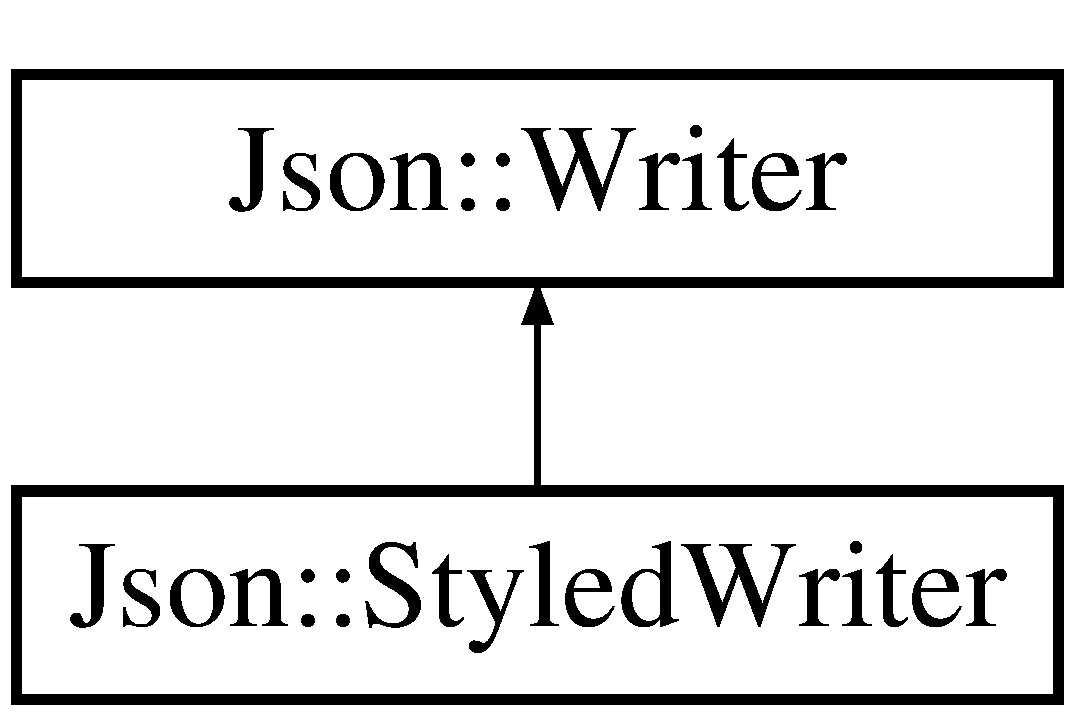
\includegraphics[height=2.000000cm]{class_json_1_1_styled_writer}
\end{center}
\end{figure}
\subsection*{Public Member Functions}
\begin{DoxyCompactItemize}
\item 
\hyperlink{class_json_1_1_styled_writer_a1f1b5f922a6a0ef0e56c6dd2f6170192}{Styled\-Writer} ()
\item 
virtual \hyperlink{class_json_1_1_styled_writer_a7eb58eabb70c6b80ac1ccec93c0c8602}{$\sim$\-Styled\-Writer} ()
\item 
virtual std\-::string \hyperlink{class_json_1_1_styled_writer_a56f0fd80f60272b3f3c85690aae66e7d}{write} (const \hyperlink{class_json_1_1_value}{Value} \&root)
\begin{DoxyCompactList}\small\item\em Serialize a \hyperlink{class_json_1_1_value}{Value} in \href{http://www.json.org}{\tt J\-S\-O\-N} format. \end{DoxyCompactList}\end{DoxyCompactItemize}


\subsection{Detailed Description}
Writes a \hyperlink{class_json_1_1_value}{Value} in \href{http://www.json.org}{\tt J\-S\-O\-N} format in a human friendly way. 

The rules for line break and indent are as follow\-:
\begin{DoxyItemize}
\item Object value\-:
\begin{DoxyItemize}
\item if empty then print \{\} without indent and line break
\item if not empty the print '\{', line break \& indent, print one value per line and then unindent and line break and print '\}'.
\end{DoxyItemize}
\item Array value\-:
\begin{DoxyItemize}
\item if empty then print \mbox{[}\mbox{]} without indent and line break
\item if the array contains no object value, empty array or some other value types, and all the values fit on one lines, then print the array on a single line.
\item otherwise, it the values do not fit on one line, or the array contains object or non empty array, then print one value per line.
\end{DoxyItemize}
\end{DoxyItemize}

If the \hyperlink{class_json_1_1_value}{Value} have comments then they are outputed according to their \hyperlink{namespace_json_a4fc417c23905b2ae9e2c47d197a45351}{Comment\-Placement}.

\begin{DoxySeeAlso}{See Also}
\hyperlink{class_json_1_1_reader}{Reader}, \hyperlink{class_json_1_1_value}{Value}, \hyperlink{class_json_1_1_value_a29f3a30f7e5d3af6f38d57999bf5b480}{Value\-::set\-Comment()} 
\end{DoxySeeAlso}


Definition at line 1852 of file json.\-hpp.



\subsection{Constructor \& Destructor Documentation}
\hypertarget{class_json_1_1_styled_writer_a1f1b5f922a6a0ef0e56c6dd2f6170192}{\index{Json\-::\-Styled\-Writer@{Json\-::\-Styled\-Writer}!Styled\-Writer@{Styled\-Writer}}
\index{Styled\-Writer@{Styled\-Writer}!Json::StyledWriter@{Json\-::\-Styled\-Writer}}
\subsubsection[{Styled\-Writer}]{\setlength{\rightskip}{0pt plus 5cm}Json\-::\-Styled\-Writer\-::\-Styled\-Writer (
\begin{DoxyParamCaption}
{}
\end{DoxyParamCaption}
)}}\label{class_json_1_1_styled_writer_a1f1b5f922a6a0ef0e56c6dd2f6170192}


Definition at line 3213 of file json.\-cpp.

\hypertarget{class_json_1_1_styled_writer_a7eb58eabb70c6b80ac1ccec93c0c8602}{\index{Json\-::\-Styled\-Writer@{Json\-::\-Styled\-Writer}!$\sim$\-Styled\-Writer@{$\sim$\-Styled\-Writer}}
\index{$\sim$\-Styled\-Writer@{$\sim$\-Styled\-Writer}!Json::StyledWriter@{Json\-::\-Styled\-Writer}}
\subsubsection[{$\sim$\-Styled\-Writer}]{\setlength{\rightskip}{0pt plus 5cm}virtual Json\-::\-Styled\-Writer\-::$\sim$\-Styled\-Writer (
\begin{DoxyParamCaption}
{}
\end{DoxyParamCaption}
)\hspace{0.3cm}{\ttfamily [inline]}, {\ttfamily [virtual]}}}\label{class_json_1_1_styled_writer_a7eb58eabb70c6b80ac1ccec93c0c8602}


Definition at line 1855 of file json.\-hpp.



\subsection{Member Function Documentation}
\hypertarget{class_json_1_1_styled_writer_a56f0fd80f60272b3f3c85690aae66e7d}{\index{Json\-::\-Styled\-Writer@{Json\-::\-Styled\-Writer}!write@{write}}
\index{write@{write}!Json::StyledWriter@{Json\-::\-Styled\-Writer}}
\subsubsection[{write}]{\setlength{\rightskip}{0pt plus 5cm}std\-::string Json\-::\-Styled\-Writer\-::write (
\begin{DoxyParamCaption}
\item[{const {\bf Value} \&}]{root}
\end{DoxyParamCaption}
)\hspace{0.3cm}{\ttfamily [virtual]}}}\label{class_json_1_1_styled_writer_a56f0fd80f60272b3f3c85690aae66e7d}


Serialize a \hyperlink{class_json_1_1_value}{Value} in \href{http://www.json.org}{\tt J\-S\-O\-N} format. 


\begin{DoxyParams}{Parameters}
{\em root} & \hyperlink{class_json_1_1_value}{Value} to serialize. \\
\hline
\end{DoxyParams}
\begin{DoxyReturn}{Returns}
String containing the J\-S\-O\-N document that represents the root value. 
\end{DoxyReturn}


Implements \hyperlink{class_json_1_1_writer_a7b2273a4ffd6f32b369ac8a53b7b5a0d}{Json\-::\-Writer}.



Definition at line 3216 of file json.\-cpp.



The documentation for this class was generated from the following files\-:\begin{DoxyCompactItemize}
\item 
includes/util/json/\hyperlink{json_8hpp}{json.\-hpp}\item 
src/util/json/\hyperlink{json_8cpp}{json.\-cpp}\end{DoxyCompactItemize}

\hypertarget{classamon_1_1_tweet_loader}{\section{amon\-:\-:Tweet\-Loader Class Reference}
\label{classamon_1_1_tweet_loader}\index{amon\-::\-Tweet\-Loader@{amon\-::\-Tweet\-Loader}}
}


{\ttfamily \#include $<$twitter.\-hpp$>$}

\subsection*{Public Types}
\begin{DoxyCompactItemize}
\item 
enum \hyperlink{classamon_1_1_tweet_loader_ad125f05eb6d11acbdc8adf728d98f085}{Network\-Type} \{ \hyperlink{classamon_1_1_tweet_loader_ad125f05eb6d11acbdc8adf728d98f085a7728c489e3955f983f00b01622b43fb7}{F\-O\-L\-L\-O\-W\-I\-N\-G\-\_\-\-N\-E\-T\-W\-O\-R\-K}, 
\hyperlink{classamon_1_1_tweet_loader_ad125f05eb6d11acbdc8adf728d98f085a81ee659193460eb810f82b0ebc062e1f}{H\-A\-S\-H\-T\-A\-G\-\_\-\-N\-E\-T\-W\-O\-R\-K}
 \}
\end{DoxyCompactItemize}
\subsection*{Public Member Functions}
\begin{DoxyCompactItemize}
\item 
\hyperlink{classamon_1_1_tweet_loader_a5448a36953241e1d2d9b0c5d8b2712ff}{Tweet\-Loader} (std\-::string json\-File, double p, \hyperlink{classamon_1_1_tweet_loader_ad125f05eb6d11acbdc8adf728d98f085}{Network\-Type} type)
\begin{DoxyCompactList}\small\item\em \{ Constructor \} \end{DoxyCompactList}\item 
\hyperlink{classamon_1_1_graph}{amon\-::\-Graph} \hyperlink{classamon_1_1_tweet_loader_a292bc02ccb78e803ef5b1f84d713ea57}{get\-Social\-Network} ()
\begin{DoxyCompactList}\small\item\em \{ Returns the loaded network. \} \end{DoxyCompactList}\end{DoxyCompactItemize}


\subsection{Detailed Description}


Definition at line 19 of file twitter.\-hpp.



\subsection{Member Enumeration Documentation}
\hypertarget{classamon_1_1_tweet_loader_ad125f05eb6d11acbdc8adf728d98f085}{\index{amon\-::\-Tweet\-Loader@{amon\-::\-Tweet\-Loader}!Network\-Type@{Network\-Type}}
\index{Network\-Type@{Network\-Type}!amon::TweetLoader@{amon\-::\-Tweet\-Loader}}
\subsubsection[{Network\-Type}]{\setlength{\rightskip}{0pt plus 5cm}enum {\bf amon\-::\-Tweet\-Loader\-::\-Network\-Type}}}\label{classamon_1_1_tweet_loader_ad125f05eb6d11acbdc8adf728d98f085}
\begin{Desc}
\item[Enumerator]\par
\begin{description}
\index{F\-O\-L\-L\-O\-W\-I\-N\-G\-\_\-\-N\-E\-T\-W\-O\-R\-K@{F\-O\-L\-L\-O\-W\-I\-N\-G\-\_\-\-N\-E\-T\-W\-O\-R\-K}!amon\-::\-Tweet\-Loader@{amon\-::\-Tweet\-Loader}}\index{amon\-::\-Tweet\-Loader@{amon\-::\-Tweet\-Loader}!F\-O\-L\-L\-O\-W\-I\-N\-G\-\_\-\-N\-E\-T\-W\-O\-R\-K@{F\-O\-L\-L\-O\-W\-I\-N\-G\-\_\-\-N\-E\-T\-W\-O\-R\-K}}\item[{\em 
\hypertarget{classamon_1_1_tweet_loader_ad125f05eb6d11acbdc8adf728d98f085a7728c489e3955f983f00b01622b43fb7}{F\-O\-L\-L\-O\-W\-I\-N\-G\-\_\-\-N\-E\-T\-W\-O\-R\-K}\label{classamon_1_1_tweet_loader_ad125f05eb6d11acbdc8adf728d98f085a7728c489e3955f983f00b01622b43fb7}
}]\index{H\-A\-S\-H\-T\-A\-G\-\_\-\-N\-E\-T\-W\-O\-R\-K@{H\-A\-S\-H\-T\-A\-G\-\_\-\-N\-E\-T\-W\-O\-R\-K}!amon\-::\-Tweet\-Loader@{amon\-::\-Tweet\-Loader}}\index{amon\-::\-Tweet\-Loader@{amon\-::\-Tweet\-Loader}!H\-A\-S\-H\-T\-A\-G\-\_\-\-N\-E\-T\-W\-O\-R\-K@{H\-A\-S\-H\-T\-A\-G\-\_\-\-N\-E\-T\-W\-O\-R\-K}}\item[{\em 
\hypertarget{classamon_1_1_tweet_loader_ad125f05eb6d11acbdc8adf728d98f085a81ee659193460eb810f82b0ebc062e1f}{H\-A\-S\-H\-T\-A\-G\-\_\-\-N\-E\-T\-W\-O\-R\-K}\label{classamon_1_1_tweet_loader_ad125f05eb6d11acbdc8adf728d98f085a81ee659193460eb810f82b0ebc062e1f}
}]\end{description}
\end{Desc}


Definition at line 22 of file twitter.\-hpp.



\subsection{Constructor \& Destructor Documentation}
\hypertarget{classamon_1_1_tweet_loader_a5448a36953241e1d2d9b0c5d8b2712ff}{\index{amon\-::\-Tweet\-Loader@{amon\-::\-Tweet\-Loader}!Tweet\-Loader@{Tweet\-Loader}}
\index{Tweet\-Loader@{Tweet\-Loader}!amon::TweetLoader@{amon\-::\-Tweet\-Loader}}
\subsubsection[{Tweet\-Loader}]{\setlength{\rightskip}{0pt plus 5cm}amon\-::\-Tweet\-Loader\-::\-Tweet\-Loader (
\begin{DoxyParamCaption}
\item[{std\-::string}]{json\-File, }
\item[{double}]{p, }
\item[{{\bf Network\-Type}}]{type}
\end{DoxyParamCaption}
)}}\label{classamon_1_1_tweet_loader_a5448a36953241e1d2d9b0c5d8b2712ff}


\{ Constructor \} 


\begin{DoxyParams}[1]{Parameters}
\mbox{\tt in}  & {\em json\-File} & \{ Path to the file containing json tweets by line. \} \\
\hline
\mbox{\tt in}  & {\em p} & \{ The percentage of the input file to load. \} \\
\hline
\end{DoxyParams}


Definition at line 51 of file twitter.\-cpp.



\subsection{Member Function Documentation}
\hypertarget{classamon_1_1_tweet_loader_a292bc02ccb78e803ef5b1f84d713ea57}{\index{amon\-::\-Tweet\-Loader@{amon\-::\-Tweet\-Loader}!get\-Social\-Network@{get\-Social\-Network}}
\index{get\-Social\-Network@{get\-Social\-Network}!amon::TweetLoader@{amon\-::\-Tweet\-Loader}}
\subsubsection[{get\-Social\-Network}]{\setlength{\rightskip}{0pt plus 5cm}{\bf amon\-::\-Graph} amon\-::\-Tweet\-Loader\-::get\-Social\-Network (
\begin{DoxyParamCaption}
{}
\end{DoxyParamCaption}
)}}\label{classamon_1_1_tweet_loader_a292bc02ccb78e803ef5b1f84d713ea57}


\{ Returns the loaded network. \} 

\begin{DoxyReturn}{Returns}
\{ An \hyperlink{classamon_1_1_graph}{amon\-::\-Graph} containing the loaded network. \} 
\end{DoxyReturn}


Definition at line 8 of file twitter.\-cpp.



The documentation for this class was generated from the following files\-:\begin{DoxyCompactItemize}
\item 
includes/social/\hyperlink{twitter_8hpp}{twitter.\-hpp}\item 
src/social/\hyperlink{twitter_8cpp}{twitter.\-cpp}\end{DoxyCompactItemize}

\hypertarget{class_json_1_1_value}{\section{Json\-:\-:Value Class Reference}
\label{class_json_1_1_value}\index{Json\-::\-Value@{Json\-::\-Value}}
}


Represents a \href{http://www.json.org}{\tt J\-S\-O\-N} value.  




{\ttfamily \#include $<$json.\-hpp$>$}

\subsection*{Public Types}
\begin{DoxyCompactItemize}
\item 
typedef std\-::vector$<$ std\-::string $>$ \hyperlink{class_json_1_1_value_ac61bab5a465848b57610379cc07995c3}{Members}
\item 
typedef \hyperlink{class_json_1_1_value_iterator}{Value\-Iterator} \hyperlink{class_json_1_1_value_a341cdf2e01f8b3c5b7317aa2f0768c53}{iterator}
\item 
typedef \hyperlink{class_json_1_1_value_const_iterator}{Value\-Const\-Iterator} \hyperlink{class_json_1_1_value_af92282ca92b58b320debd486afb7696a}{const\-\_\-iterator}
\item 
typedef \hyperlink{namespace_json_a800fb90eb6ee8d5d62b600c06f87f7d4}{Json\-::\-U\-Int} \hyperlink{class_json_1_1_value_a0933d59b45793ae4aade1757c322a98d}{U\-Int}
\item 
typedef \hyperlink{namespace_json_a08122e8005b706d982e48cca1e2119c7}{Json\-::\-Int} \hyperlink{class_json_1_1_value_abdf7a7ff73eb130ffcab28504ffdb405}{Int}
\item 
typedef \hyperlink{namespace_json_a01f20bce8f8229f38ff890168c0e6452}{Json\-::\-U\-Int64} \hyperlink{class_json_1_1_value_a8b62564be8c087c6d18de180ff4e13e3}{U\-Int64}
\item 
typedef \hyperlink{namespace_json_ab7b47d2905da3b4ae60e4e800ec9ae5f}{Json\-::\-Int64} \hyperlink{class_json_1_1_value_a1b86af9f85f0f1baa972c3319fa22695}{Int64}
\item 
typedef \hyperlink{namespace_json_a218d880af853ce786cd985e82571d297}{Json\-::\-Largest\-Int} \hyperlink{class_json_1_1_value_a1cbb82642ed05109b9833e49f042ece7}{Largest\-Int}
\item 
typedef \hyperlink{namespace_json_ae202ecad69725e23443f465e257456d0}{Json\-::\-Largest\-U\-Int} \hyperlink{class_json_1_1_value_a6682a3684d635e03fc06ba229fa24eec}{Largest\-U\-Int}
\item 
typedef \hyperlink{namespace_json_a8048e741f2177c3b5d9ede4a5b8c53c2}{Json\-::\-Array\-Index} \hyperlink{class_json_1_1_value_a184a91566cccca7b819240f0d5561c7d}{Array\-Index}
\item 
typedef std\-::map$<$ C\-Z\-String, \hyperlink{class_json_1_1_value}{Value} $>$ \hyperlink{class_json_1_1_value_a08b6c80c3af7071d908dabf044de5388}{Object\-Values}
\end{DoxyCompactItemize}
\subsection*{Public Member Functions}
\begin{DoxyCompactItemize}
\item 
\hyperlink{class_json_1_1_value_ada6ba1369448fb0240bccc36efaa46f7}{Value} (\hyperlink{namespace_json_a7d654b75c16a57007925868e38212b4e}{Value\-Type} \hyperlink{class_json_1_1_value_a695ef31fad36b4712918b3ff80158479}{type}=\hyperlink{namespace_json_a7d654b75c16a57007925868e38212b4ea7d9899633b4409bd3fc107e6737f8391}{null\-Value})
\begin{DoxyCompactList}\small\item\em Create a default \hyperlink{class_json_1_1_value}{Value} of the given type. \end{DoxyCompactList}\item 
\hyperlink{class_json_1_1_value_a4744ae571fcf34f4b16a2257b3b3b585}{Value} (\hyperlink{class_json_1_1_value_abdf7a7ff73eb130ffcab28504ffdb405}{Int} value)
\item 
\hyperlink{class_json_1_1_value_ae67a857b01286e3499a87e95be848d20}{Value} (\hyperlink{class_json_1_1_value_a0933d59b45793ae4aade1757c322a98d}{U\-Int} value)
\item 
\hyperlink{class_json_1_1_value_ab1cdc3d9a4d4cc03fa01439d43ceb1b5}{Value} (\hyperlink{class_json_1_1_value_a1b86af9f85f0f1baa972c3319fa22695}{Int64} value)
\item 
\hyperlink{class_json_1_1_value_a8adda58d5ae17bf7ca6a53bab4a7b69c}{Value} (\hyperlink{class_json_1_1_value_a8b62564be8c087c6d18de180ff4e13e3}{U\-Int64} value)
\item 
\hyperlink{class_json_1_1_value_a32228cc84d83200cca8441451997996c}{Value} (double value)
\item 
\hyperlink{class_json_1_1_value_ad87b849356816aca75995dd07302e49d}{Value} (const char $\ast$value)
\item 
\hyperlink{class_json_1_1_value_a13e567d467bb1e699d71e27a76b0e988}{Value} (const char $\ast$begin\-Value, const char $\ast$end\-Value)
\item 
\hyperlink{class_json_1_1_value_a081830e95f88a37054da7e46c65b0766}{Value} (const \hyperlink{class_json_1_1_static_string}{Static\-String} \&value)
\begin{DoxyCompactList}\small\item\em Constructs a value from a static string. \end{DoxyCompactList}\item 
\hyperlink{class_json_1_1_value_aa4501dd4edf3ce3d5145fc656f088b21}{Value} (const std\-::string \&value)
\item 
\hyperlink{class_json_1_1_value_a350a31ea4a30d384994b0bc010b17495}{Value} (bool value)
\item 
\hyperlink{class_json_1_1_value_a436dfd3670f95fd665f680eba5cebcf0}{Value} (const \hyperlink{class_json_1_1_value}{Value} \&other)
\item 
\hyperlink{class_json_1_1_value_a287dea48da3912d02756735bf677b27b}{$\sim$\-Value} ()
\item 
\hyperlink{class_json_1_1_value}{Value} \& \hyperlink{class_json_1_1_value_a795acb28772da4c5d85ae8f4af36c69f}{operator=} (\hyperlink{class_json_1_1_value}{Value} other)
\item 
void \hyperlink{class_json_1_1_value_aab841120d78e296e1bc06a373345e822}{swap} (\hyperlink{class_json_1_1_value}{Value} \&other)
\item 
\hyperlink{namespace_json_a7d654b75c16a57007925868e38212b4e}{Value\-Type} \hyperlink{class_json_1_1_value_a695ef31fad36b4712918b3ff80158479}{type} () const 
\item 
bool \hyperlink{class_json_1_1_value_af0ad8aa027575c3277296458f3fb7b0a}{operator$<$} (const \hyperlink{class_json_1_1_value}{Value} \&other) const 
\item 
bool \hyperlink{class_json_1_1_value_afb99dd3628fe44244b32007f9b4f369a}{operator$<$=} (const \hyperlink{class_json_1_1_value}{Value} \&other) const 
\item 
bool \hyperlink{class_json_1_1_value_acc13fc47d55abd6e2327b090b83d2911}{operator$>$=} (const \hyperlink{class_json_1_1_value}{Value} \&other) const 
\item 
bool \hyperlink{class_json_1_1_value_a3124a26067bdfde9571bc89527fc6931}{operator$>$} (const \hyperlink{class_json_1_1_value}{Value} \&other) const 
\item 
bool \hyperlink{class_json_1_1_value_a14363dda23a6ae2def9afd1590ae85d3}{operator==} (const \hyperlink{class_json_1_1_value}{Value} \&other) const 
\item 
bool \hyperlink{class_json_1_1_value_ad0f12d2a4ab74bbef08a05504b2cb81d}{operator!=} (const \hyperlink{class_json_1_1_value}{Value} \&other) const 
\item 
int \hyperlink{class_json_1_1_value_a899214ed2253d3f4f061b922b0e622b5}{compare} (const \hyperlink{class_json_1_1_value}{Value} \&other) const 
\item 
const char $\ast$ \hyperlink{class_json_1_1_value_a5b7da48b163bcec63b1424f1608b7da6}{as\-C\-String} () const 
\item 
std\-::string \hyperlink{class_json_1_1_value_a03ee3d5df576640c93ba683f140828bd}{as\-String} () const 
\item 
\hyperlink{class_json_1_1_value_abdf7a7ff73eb130ffcab28504ffdb405}{Int} \hyperlink{class_json_1_1_value_ac786e35b860b1d700cb3d3e56dd6a235}{as\-Int} () const 
\item 
\hyperlink{class_json_1_1_value_a0933d59b45793ae4aade1757c322a98d}{U\-Int} \hyperlink{class_json_1_1_value_a2019d1bd296b89356c1b0da5970c918c}{as\-U\-Int} () const 
\item 
\hyperlink{class_json_1_1_value_a1b86af9f85f0f1baa972c3319fa22695}{Int64} \hyperlink{class_json_1_1_value_a4451cee7524534458894f4e2cc045aa3}{as\-Int64} () const 
\item 
\hyperlink{class_json_1_1_value_a8b62564be8c087c6d18de180ff4e13e3}{U\-Int64} \hyperlink{class_json_1_1_value_a4aa617bc0625ae0f208fa54b7c6326ad}{as\-U\-Int64} () const 
\item 
\hyperlink{class_json_1_1_value_a1cbb82642ed05109b9833e49f042ece7}{Largest\-Int} \hyperlink{class_json_1_1_value_a3786bb100c5cf9a98eb6d13784968956}{as\-Largest\-Int} () const 
\item 
\hyperlink{class_json_1_1_value_a6682a3684d635e03fc06ba229fa24eec}{Largest\-U\-Int} \hyperlink{class_json_1_1_value_a692b88345a745b2f89ca5d94b52e94d4}{as\-Largest\-U\-Int} () const 
\item 
float \hyperlink{class_json_1_1_value_ac2128d7080499daf8c5b1c71da243f63}{as\-Float} () const 
\item 
double \hyperlink{class_json_1_1_value_a33434ed1c0217a34d04c95fa5342fd37}{as\-Double} () const 
\item 
bool \hyperlink{class_json_1_1_value_a7402c797285c020566c3db5f8ae4e940}{as\-Bool} () const 
\item 
bool \hyperlink{class_json_1_1_value_aeb9ad8b1bb91bdd72203dc884b3f4362}{is\-Null} () const 
\item 
bool \hyperlink{class_json_1_1_value_a3c3716cc7a0216cb1b654bb8f61c8d13}{is\-Bool} () const 
\item 
bool \hyperlink{class_json_1_1_value_ab0df4746d6787d2ce1db1a156c118f14}{is\-Int} () const 
\item 
bool \hyperlink{class_json_1_1_value_aba89690e5fd72d0f7121a30013470423}{is\-Int64} () const 
\item 
bool \hyperlink{class_json_1_1_value_ae814ca1796fe2d43ac09898b70213989}{is\-U\-Int} () const 
\item 
bool \hyperlink{class_json_1_1_value_aa35efece2a6cba4d988d7d5b54db2fb8}{is\-U\-Int64} () const 
\item 
bool \hyperlink{class_json_1_1_value_aec4f74ef7b776b1d9c8a10fc3bb4add5}{is\-Integral} () const 
\item 
bool \hyperlink{class_json_1_1_value_a0ea567fa51fc808851698bef59b43626}{is\-Double} () const 
\item 
bool \hyperlink{class_json_1_1_value_a8ce848900e2e8fa23a41fcc2c1409fab}{is\-Numeric} () const 
\item 
bool \hyperlink{class_json_1_1_value_a06c01d7c1e8151a5844b595ab00f46c7}{is\-String} () const 
\item 
bool \hyperlink{class_json_1_1_value_ac8c898f93543e55b67418f94bced20af}{is\-Array} () const 
\item 
bool \hyperlink{class_json_1_1_value_a80cffaa0402b80317c0437216bbb6d92}{is\-Object} () const 
\item 
bool \hyperlink{class_json_1_1_value_a7ec153803631a27abf58cba2bb1af70c}{is\-Convertible\-To} (\hyperlink{namespace_json_a7d654b75c16a57007925868e38212b4e}{Value\-Type} other) const 
\item 
\hyperlink{class_json_1_1_value_a184a91566cccca7b819240f0d5561c7d}{Array\-Index} \hyperlink{class_json_1_1_value_a4ca8ee6c48a34ca6c2f131956bab5e05}{size} () const 
\begin{DoxyCompactList}\small\item\em Number of values in array or object. \end{DoxyCompactList}\item 
bool \hyperlink{class_json_1_1_value_a99c42d3ff8495dad1e91b43e66553c36}{empty} () const 
\begin{DoxyCompactList}\small\item\em Return true if empty array, empty object, or null; otherwise, false. \end{DoxyCompactList}\item 
bool \hyperlink{class_json_1_1_value_a021ab0d15a807fbe051446c9c545ab61}{operator!} () const 
\begin{DoxyCompactList}\small\item\em Return \hyperlink{class_json_1_1_value_aeb9ad8b1bb91bdd72203dc884b3f4362}{is\-Null()} \end{DoxyCompactList}\item 
void \hyperlink{class_json_1_1_value_a501a4d67e6c875255c2ecc03ccd2019b}{clear} ()
\item 
void \hyperlink{class_json_1_1_value_aa284353271ada427dbfa04a42f2be407}{resize} (\hyperlink{class_json_1_1_value_a184a91566cccca7b819240f0d5561c7d}{Array\-Index} \hyperlink{class_json_1_1_value_a4ca8ee6c48a34ca6c2f131956bab5e05}{size})
\item 
\hyperlink{class_json_1_1_value}{Value} \& \hyperlink{class_json_1_1_value_a7d99f5dba388cdaa152ce6ef933d64ef}{operator\mbox{[}$\,$\mbox{]}} (\hyperlink{class_json_1_1_value_a184a91566cccca7b819240f0d5561c7d}{Array\-Index} index)
\item 
\hyperlink{class_json_1_1_value}{Value} \& \hyperlink{class_json_1_1_value_ac9182982c361e0ab621134d406e5f250}{operator\mbox{[}$\,$\mbox{]}} (int index)
\item 
const \hyperlink{class_json_1_1_value}{Value} \& \hyperlink{class_json_1_1_value_af151919e8947c430e34bed2b0b128601}{operator\mbox{[}$\,$\mbox{]}} (\hyperlink{class_json_1_1_value_a184a91566cccca7b819240f0d5561c7d}{Array\-Index} index) const 
\item 
const \hyperlink{class_json_1_1_value}{Value} \& \hyperlink{class_json_1_1_value_af9e02b38f4e63e491c300c20b275bdd7}{operator\mbox{[}$\,$\mbox{]}} (int index) const 
\item 
\hyperlink{class_json_1_1_value}{Value} \hyperlink{class_json_1_1_value_a28282c9b76fa031eba7a1843c47c16fe}{get} (\hyperlink{class_json_1_1_value_a184a91566cccca7b819240f0d5561c7d}{Array\-Index} index, const \hyperlink{class_json_1_1_value}{Value} \&default\-Value) const 
\item 
bool \hyperlink{class_json_1_1_value_aaa82ebb4b730ea1567d310874f47d147}{is\-Valid\-Index} (\hyperlink{class_json_1_1_value_a184a91566cccca7b819240f0d5561c7d}{Array\-Index} index) const 
\begin{DoxyCompactList}\small\item\em Return true if index $<$ \hyperlink{class_json_1_1_value_a4ca8ee6c48a34ca6c2f131956bab5e05}{size()}. \end{DoxyCompactList}\item 
\hyperlink{class_json_1_1_value}{Value} \& \hyperlink{class_json_1_1_value_a7e49ac977e4bcf59745a09d426669f75}{append} (const \hyperlink{class_json_1_1_value}{Value} \&value)
\begin{DoxyCompactList}\small\item\em Append value to array at the end. \end{DoxyCompactList}\item 
\hyperlink{class_json_1_1_value}{Value} \& \hyperlink{class_json_1_1_value_acb912f4ec40a25ea6eb387730885f3d9}{operator\mbox{[}$\,$\mbox{]}} (const char $\ast$key)
\begin{DoxyCompactList}\small\item\em Access an object value by name, create a null member if it does not exist. \end{DoxyCompactList}\item 
const \hyperlink{class_json_1_1_value}{Value} \& \hyperlink{class_json_1_1_value_ae5f73ffc7a039bca81b7ca771bc5db55}{operator\mbox{[}$\,$\mbox{]}} (const char $\ast$key) const 
\item 
\hyperlink{class_json_1_1_value}{Value} \& \hyperlink{class_json_1_1_value_ae511c7d46bf457412fb55c9471af9f50}{operator\mbox{[}$\,$\mbox{]}} (const std\-::string \&key)
\begin{DoxyCompactList}\small\item\em Access an object value by name, create a null member if it does not exist. \end{DoxyCompactList}\item 
const \hyperlink{class_json_1_1_value}{Value} \& \hyperlink{class_json_1_1_value_ac14123afaf12d953aad75ec2610fbb85}{operator\mbox{[}$\,$\mbox{]}} (const std\-::string \&key) const 
\item 
\hyperlink{class_json_1_1_value}{Value} \& \hyperlink{class_json_1_1_value_ac3763d7d315ca65dc188e273722f7955}{operator\mbox{[}$\,$\mbox{]}} (const \hyperlink{class_json_1_1_static_string}{Static\-String} \&key)
\begin{DoxyCompactList}\small\item\em Access an object value by name, create a null member if it does not exist. \end{DoxyCompactList}\item 
\hyperlink{class_json_1_1_value}{Value} \hyperlink{class_json_1_1_value_ab76b3323cde14c7db20676d07b260ce7}{get} (const char $\ast$key, const \hyperlink{class_json_1_1_value}{Value} \&default\-Value) const 
\begin{DoxyCompactList}\small\item\em Return the member named key if it exist, default\-Value otherwise. \end{DoxyCompactList}\item 
\hyperlink{class_json_1_1_value}{Value} \hyperlink{class_json_1_1_value_a54a34264356e01ee9c21a75ccfc809e9}{get} (const std\-::string \&key, const \hyperlink{class_json_1_1_value}{Value} \&default\-Value) const 
\begin{DoxyCompactList}\small\item\em Return the member named key if it exist, default\-Value otherwise. \end{DoxyCompactList}\item 
\hyperlink{class_json_1_1_value}{Value} \hyperlink{class_json_1_1_value_aa52f7873b95d29627d6e83ba96f69aaa}{remove\-Member} (const char $\ast$key)
\begin{DoxyCompactList}\small\item\em Remove and return the named member. \end{DoxyCompactList}\item 
\hyperlink{class_json_1_1_value}{Value} \hyperlink{class_json_1_1_value_ae1f95f7ca3906e6bcc2a7be93210ecba}{remove\-Member} (const std\-::string \&key)
\begin{DoxyCompactList}\small\item\em Same as \hyperlink{class_json_1_1_value_aa52f7873b95d29627d6e83ba96f69aaa}{remove\-Member(const char$\ast$)} \end{DoxyCompactList}\item 
bool \hyperlink{class_json_1_1_value_a196defba501d70ea2b6793afb04108e3}{is\-Member} (const char $\ast$key) const 
\begin{DoxyCompactList}\small\item\em Return true if the object has a member named key. \end{DoxyCompactList}\item 
bool \hyperlink{class_json_1_1_value_af728b5738aaa133f3aad2e39dc4f415e}{is\-Member} (const std\-::string \&key) const 
\begin{DoxyCompactList}\small\item\em Return true if the object has a member named key. \end{DoxyCompactList}\item 
\hyperlink{class_json_1_1_value_ac61bab5a465848b57610379cc07995c3}{Members} \hyperlink{class_json_1_1_value_a30fa08af88f2d0a038b22ba9f4e88b2a}{get\-Member\-Names} () const 
\begin{DoxyCompactList}\small\item\em Return a list of the member names. \end{DoxyCompactList}\item 
void \hyperlink{class_json_1_1_value_a29f3a30f7e5d3af6f38d57999bf5b480}{set\-Comment} (const char $\ast$comment, \hyperlink{namespace_json_a4fc417c23905b2ae9e2c47d197a45351}{Comment\-Placement} placement)
\begin{DoxyCompactList}\small\item\em Comments must be //... or /$\ast$ ... $\ast$/. \end{DoxyCompactList}\item 
void \hyperlink{class_json_1_1_value_a6d68a2e7d4e1e317cd9e812e12181689}{set\-Comment} (const std\-::string \&comment, \hyperlink{namespace_json_a4fc417c23905b2ae9e2c47d197a45351}{Comment\-Placement} placement)
\begin{DoxyCompactList}\small\item\em Comments must be //... or /$\ast$ ... $\ast$/. \end{DoxyCompactList}\item 
bool \hyperlink{class_json_1_1_value_a06567a00363cab9601be7e31336db03a}{has\-Comment} (\hyperlink{namespace_json_a4fc417c23905b2ae9e2c47d197a45351}{Comment\-Placement} placement) const 
\item 
std\-::string \hyperlink{class_json_1_1_value_aa1e105b5d7f55d6e42f4fb2f3674116f}{get\-Comment} (\hyperlink{namespace_json_a4fc417c23905b2ae9e2c47d197a45351}{Comment\-Placement} placement) const 
\begin{DoxyCompactList}\small\item\em Include delimiters and embedded newlines. \end{DoxyCompactList}\item 
std\-::string \hyperlink{class_json_1_1_value_a05357cf78959b790337fae4e5580ee4f}{to\-Styled\-String} () const 
\item 
\hyperlink{class_json_1_1_value_af92282ca92b58b320debd486afb7696a}{const\-\_\-iterator} \hyperlink{class_json_1_1_value_ac12df0d6980600c5bac908ed0f64856e}{begin} () const 
\item 
\hyperlink{class_json_1_1_value_af92282ca92b58b320debd486afb7696a}{const\-\_\-iterator} \hyperlink{class_json_1_1_value_a596da1926b2f2a4056bff2edb713eb0b}{end} () const 
\item 
\hyperlink{class_json_1_1_value_a341cdf2e01f8b3c5b7317aa2f0768c53}{iterator} \hyperlink{class_json_1_1_value_a2d45bb2e68e8f22fe356d7d955ebd3c9}{begin} ()
\item 
\hyperlink{class_json_1_1_value_a341cdf2e01f8b3c5b7317aa2f0768c53}{iterator} \hyperlink{class_json_1_1_value_a2f961eff73f7f79cd29260b6cbd42558}{end} ()
\item 
void \hyperlink{class_json_1_1_value_a6d741407c3d784360c200f181b0d6d64}{set\-Offset\-Start} (size\-\_\-t start)
\item 
void \hyperlink{class_json_1_1_value_ac6d858b5fd4d5fe6ca84f697def8c5ea}{set\-Offset\-Limit} (size\-\_\-t limit)
\item 
size\-\_\-t \hyperlink{class_json_1_1_value_a10142eda11ae0b1caecbcc9f436854d1}{get\-Offset\-Start} () const 
\item 
size\-\_\-t \hyperlink{class_json_1_1_value_acd7114469bc39368e9d93c29b54d8c8f}{get\-Offset\-Limit} () const 
\end{DoxyCompactItemize}
\subsection*{Static Public Attributes}
\begin{DoxyCompactItemize}
\item 
static const \hyperlink{class_json_1_1_value}{Value} \& \hyperlink{class_json_1_1_value_a6d6e9ea6807e46d5b7ded66d3032f607}{null} = reinterpret\-\_\-cast$<$const \hyperlink{class_json_1_1_value}{Value}\&$>$(\hyperlink{namespace_json_ab30055b4bbd82aecaca57ccecd63bbe6}{k\-Null\-Ref})
\item 
static const \hyperlink{class_json_1_1_value_a1cbb82642ed05109b9833e49f042ece7}{Largest\-Int} \hyperlink{class_json_1_1_value_af91df130daa50dd43d2cd89e6ee67706}{min\-Largest\-Int} = \hyperlink{class_json_1_1_value_a1cbb82642ed05109b9833e49f042ece7}{Largest\-Int}($\sim$(\hyperlink{class_json_1_1_value_a6682a3684d635e03fc06ba229fa24eec}{Largest\-U\-Int}(-\/1) / 2))
\begin{DoxyCompactList}\small\item\em Minimum signed integer value that can be stored in a \hyperlink{class_json_1_1_value}{Json\-::\-Value}. \end{DoxyCompactList}\item 
static const \hyperlink{class_json_1_1_value_a1cbb82642ed05109b9833e49f042ece7}{Largest\-Int} \hyperlink{class_json_1_1_value_a8b4977696f13296fa8755c7953fafb2f}{max\-Largest\-Int} = \hyperlink{class_json_1_1_value_a1cbb82642ed05109b9833e49f042ece7}{Largest\-Int}(\hyperlink{class_json_1_1_value_a6682a3684d635e03fc06ba229fa24eec}{Largest\-U\-Int}(-\/1) / 2)
\begin{DoxyCompactList}\small\item\em Maximum signed integer value that can be stored in a \hyperlink{class_json_1_1_value}{Json\-::\-Value}. \end{DoxyCompactList}\item 
static const \hyperlink{class_json_1_1_value_a6682a3684d635e03fc06ba229fa24eec}{Largest\-U\-Int} \hyperlink{class_json_1_1_value_a8ddb32d9d55fa5323ae5135639dc2e31}{max\-Largest\-U\-Int} = \hyperlink{class_json_1_1_value_a6682a3684d635e03fc06ba229fa24eec}{Largest\-U\-Int}(-\/1)
\begin{DoxyCompactList}\small\item\em Maximum unsigned integer value that can be stored in a \hyperlink{class_json_1_1_value}{Json\-::\-Value}. \end{DoxyCompactList}\item 
static const \hyperlink{class_json_1_1_value_abdf7a7ff73eb130ffcab28504ffdb405}{Int} \hyperlink{class_json_1_1_value_a7df8a39e2502b8c92a6a41e3d752d2c8}{min\-Int} = \hyperlink{class_json_1_1_value_abdf7a7ff73eb130ffcab28504ffdb405}{Int}($\sim$(\hyperlink{class_json_1_1_value_a0933d59b45793ae4aade1757c322a98d}{U\-Int}(-\/1) / 2))
\begin{DoxyCompactList}\small\item\em Minimum signed int value that can be stored in a \hyperlink{class_json_1_1_value}{Json\-::\-Value}. \end{DoxyCompactList}\item 
static const \hyperlink{class_json_1_1_value_abdf7a7ff73eb130ffcab28504ffdb405}{Int} \hyperlink{class_json_1_1_value_a978c799a8af3114ef7dab6fd0a310a1b}{max\-Int} = \hyperlink{class_json_1_1_value_abdf7a7ff73eb130ffcab28504ffdb405}{Int}(\hyperlink{class_json_1_1_value_a0933d59b45793ae4aade1757c322a98d}{U\-Int}(-\/1) / 2)
\begin{DoxyCompactList}\small\item\em Maximum signed int value that can be stored in a \hyperlink{class_json_1_1_value}{Json\-::\-Value}. \end{DoxyCompactList}\item 
static const \hyperlink{class_json_1_1_value_a0933d59b45793ae4aade1757c322a98d}{U\-Int} \hyperlink{class_json_1_1_value_ac79e63ee68d3aa914bfd6988be669b87}{max\-U\-Int} = \hyperlink{class_json_1_1_value_a0933d59b45793ae4aade1757c322a98d}{U\-Int}(-\/1)
\begin{DoxyCompactList}\small\item\em Maximum unsigned int value that can be stored in a \hyperlink{class_json_1_1_value}{Json\-::\-Value}. \end{DoxyCompactList}\item 
static const \hyperlink{class_json_1_1_value_a1b86af9f85f0f1baa972c3319fa22695}{Int64} \hyperlink{class_json_1_1_value_a815ef899bc312c93bc426511acfe31a7}{min\-Int64}
\begin{DoxyCompactList}\small\item\em Minimum signed 64 bits int value that can be stored in a \hyperlink{class_json_1_1_value}{Json\-::\-Value}. \end{DoxyCompactList}\item 
static const \hyperlink{class_json_1_1_value_a1b86af9f85f0f1baa972c3319fa22695}{Int64} \hyperlink{class_json_1_1_value_a4492634870b8c5709ce967b384ac6006}{max\-Int64}
\begin{DoxyCompactList}\small\item\em Maximum signed 64 bits int value that can be stored in a \hyperlink{class_json_1_1_value}{Json\-::\-Value}. \end{DoxyCompactList}\item 
static const \hyperlink{class_json_1_1_value_a8b62564be8c087c6d18de180ff4e13e3}{U\-Int64} \hyperlink{class_json_1_1_value_ae1eb89c305c39516696ff305cffa01da}{max\-U\-Int64}
\begin{DoxyCompactList}\small\item\em Maximum unsigned 64 bits int value that can be stored in a \hyperlink{class_json_1_1_value}{Json\-::\-Value}. \end{DoxyCompactList}\end{DoxyCompactItemize}
\subsection*{Friends}
\begin{DoxyCompactItemize}
\item 
class \hyperlink{class_json_1_1_value_ad016df56489e5d360735457afba2f649}{Value\-Iterator\-Base}
\end{DoxyCompactItemize}


\subsection{Detailed Description}
Represents a \href{http://www.json.org}{\tt J\-S\-O\-N} value. 

This class is a discriminated union wrapper that can represents a\-:
\begin{DoxyItemize}
\item signed integer \mbox{[}range\-: \hyperlink{class_json_1_1_value_a7df8a39e2502b8c92a6a41e3d752d2c8}{Value\-::min\-Int} -\/ \hyperlink{class_json_1_1_value_a978c799a8af3114ef7dab6fd0a310a1b}{Value\-::max\-Int}\mbox{]}
\item unsigned integer (range\-: 0 -\/ \hyperlink{class_json_1_1_value_ac79e63ee68d3aa914bfd6988be669b87}{Value\-::max\-U\-Int})
\item double
\item U\-T\-F-\/8 string
\item boolean
\item 'null'
\item an ordered list of \hyperlink{class_json_1_1_value}{Value}
\item collection of name/value pairs (javascript object)
\end{DoxyItemize}

The type of the held value is represented by a \hyperlink{namespace_json_a7d654b75c16a57007925868e38212b4e}{Value\-Type} and can be obtained using \hyperlink{class_json_1_1_value_a695ef31fad36b4712918b3ff80158479}{type()}.

values of an \hyperlink{namespace_json_a7d654b75c16a57007925868e38212b4eae8386dcfc36d1ae897745f7b4f77a1f6}{object\-Value} or \hyperlink{namespace_json_a7d654b75c16a57007925868e38212b4eadc8f264f36b55b063c78126b335415f4}{array\-Value} can be accessed using \hyperlink{class_json_1_1_value_a7d99f5dba388cdaa152ce6ef933d64ef}{operator\mbox{[}$\,$\mbox{]}()} methods. Non const methods will automatically create the a \hyperlink{namespace_json_a7d654b75c16a57007925868e38212b4ea7d9899633b4409bd3fc107e6737f8391}{null\-Value} element if it does not exist. The sequence of an \hyperlink{namespace_json_a7d654b75c16a57007925868e38212b4eadc8f264f36b55b063c78126b335415f4}{array\-Value} will be automatically resize and initialized with \hyperlink{namespace_json_a7d654b75c16a57007925868e38212b4ea7d9899633b4409bd3fc107e6737f8391}{null\-Value}. \hyperlink{class_json_1_1_value_aa284353271ada427dbfa04a42f2be407}{resize()} can be used to enlarge or truncate an \hyperlink{namespace_json_a7d654b75c16a57007925868e38212b4eadc8f264f36b55b063c78126b335415f4}{array\-Value}.

The \hyperlink{class_json_1_1_value_a28282c9b76fa031eba7a1843c47c16fe}{get()} methods can be used to obtanis default value in the case the required element does not exist.

It is possible to iterate over the list of a \hyperlink{namespace_json_a7d654b75c16a57007925868e38212b4eae8386dcfc36d1ae897745f7b4f77a1f6}{object\-Value} values using the \hyperlink{class_json_1_1_value_a30fa08af88f2d0a038b22ba9f4e88b2a}{get\-Member\-Names()} method. 

Definition at line 482 of file json.\-hpp.



\subsection{Member Typedef Documentation}
\hypertarget{class_json_1_1_value_a184a91566cccca7b819240f0d5561c7d}{\index{Json\-::\-Value@{Json\-::\-Value}!Array\-Index@{Array\-Index}}
\index{Array\-Index@{Array\-Index}!Json::Value@{Json\-::\-Value}}
\subsubsection[{Array\-Index}]{\setlength{\rightskip}{0pt plus 5cm}typedef {\bf Json\-::\-Array\-Index} {\bf Json\-::\-Value\-::\-Array\-Index}}}\label{class_json_1_1_value_a184a91566cccca7b819240f0d5561c7d}


Definition at line 500 of file json.\-hpp.

\hypertarget{class_json_1_1_value_af92282ca92b58b320debd486afb7696a}{\index{Json\-::\-Value@{Json\-::\-Value}!const\-\_\-iterator@{const\-\_\-iterator}}
\index{const\-\_\-iterator@{const\-\_\-iterator}!Json::Value@{Json\-::\-Value}}
\subsubsection[{const\-\_\-iterator}]{\setlength{\rightskip}{0pt plus 5cm}typedef {\bf Value\-Const\-Iterator} {\bf Json\-::\-Value\-::const\-\_\-iterator}}}\label{class_json_1_1_value_af92282ca92b58b320debd486afb7696a}


Definition at line 491 of file json.\-hpp.

\hypertarget{class_json_1_1_value_abdf7a7ff73eb130ffcab28504ffdb405}{\index{Json\-::\-Value@{Json\-::\-Value}!Int@{Int}}
\index{Int@{Int}!Json::Value@{Json\-::\-Value}}
\subsubsection[{Int}]{\setlength{\rightskip}{0pt plus 5cm}typedef {\bf Json\-::\-Int} {\bf Json\-::\-Value\-::\-Int}}}\label{class_json_1_1_value_abdf7a7ff73eb130ffcab28504ffdb405}


Definition at line 493 of file json.\-hpp.

\hypertarget{class_json_1_1_value_a1b86af9f85f0f1baa972c3319fa22695}{\index{Json\-::\-Value@{Json\-::\-Value}!Int64@{Int64}}
\index{Int64@{Int64}!Json::Value@{Json\-::\-Value}}
\subsubsection[{Int64}]{\setlength{\rightskip}{0pt plus 5cm}typedef {\bf Json\-::\-Int64} {\bf Json\-::\-Value\-::\-Int64}}}\label{class_json_1_1_value_a1b86af9f85f0f1baa972c3319fa22695}


Definition at line 496 of file json.\-hpp.

\hypertarget{class_json_1_1_value_a341cdf2e01f8b3c5b7317aa2f0768c53}{\index{Json\-::\-Value@{Json\-::\-Value}!iterator@{iterator}}
\index{iterator@{iterator}!Json::Value@{Json\-::\-Value}}
\subsubsection[{iterator}]{\setlength{\rightskip}{0pt plus 5cm}typedef {\bf Value\-Iterator} {\bf Json\-::\-Value\-::iterator}}}\label{class_json_1_1_value_a341cdf2e01f8b3c5b7317aa2f0768c53}


Definition at line 490 of file json.\-hpp.

\hypertarget{class_json_1_1_value_a1cbb82642ed05109b9833e49f042ece7}{\index{Json\-::\-Value@{Json\-::\-Value}!Largest\-Int@{Largest\-Int}}
\index{Largest\-Int@{Largest\-Int}!Json::Value@{Json\-::\-Value}}
\subsubsection[{Largest\-Int}]{\setlength{\rightskip}{0pt plus 5cm}typedef {\bf Json\-::\-Largest\-Int} {\bf Json\-::\-Value\-::\-Largest\-Int}}}\label{class_json_1_1_value_a1cbb82642ed05109b9833e49f042ece7}


Definition at line 498 of file json.\-hpp.

\hypertarget{class_json_1_1_value_a6682a3684d635e03fc06ba229fa24eec}{\index{Json\-::\-Value@{Json\-::\-Value}!Largest\-U\-Int@{Largest\-U\-Int}}
\index{Largest\-U\-Int@{Largest\-U\-Int}!Json::Value@{Json\-::\-Value}}
\subsubsection[{Largest\-U\-Int}]{\setlength{\rightskip}{0pt plus 5cm}typedef {\bf Json\-::\-Largest\-U\-Int} {\bf Json\-::\-Value\-::\-Largest\-U\-Int}}}\label{class_json_1_1_value_a6682a3684d635e03fc06ba229fa24eec}


Definition at line 499 of file json.\-hpp.

\hypertarget{class_json_1_1_value_ac61bab5a465848b57610379cc07995c3}{\index{Json\-::\-Value@{Json\-::\-Value}!Members@{Members}}
\index{Members@{Members}!Json::Value@{Json\-::\-Value}}
\subsubsection[{Members}]{\setlength{\rightskip}{0pt plus 5cm}typedef std\-::vector$<$std\-::string$>$ {\bf Json\-::\-Value\-::\-Members}}}\label{class_json_1_1_value_ac61bab5a465848b57610379cc07995c3}


Definition at line 489 of file json.\-hpp.

\hypertarget{class_json_1_1_value_a08b6c80c3af7071d908dabf044de5388}{\index{Json\-::\-Value@{Json\-::\-Value}!Object\-Values@{Object\-Values}}
\index{Object\-Values@{Object\-Values}!Json::Value@{Json\-::\-Value}}
\subsubsection[{Object\-Values}]{\setlength{\rightskip}{0pt plus 5cm}typedef std\-::map$<$C\-Z\-String, {\bf Value}$>$ {\bf Json\-::\-Value\-::\-Object\-Values}}}\label{class_json_1_1_value_a08b6c80c3af7071d908dabf044de5388}


Definition at line 555 of file json.\-hpp.

\hypertarget{class_json_1_1_value_a0933d59b45793ae4aade1757c322a98d}{\index{Json\-::\-Value@{Json\-::\-Value}!U\-Int@{U\-Int}}
\index{U\-Int@{U\-Int}!Json::Value@{Json\-::\-Value}}
\subsubsection[{U\-Int}]{\setlength{\rightskip}{0pt plus 5cm}typedef {\bf Json\-::\-U\-Int} {\bf Json\-::\-Value\-::\-U\-Int}}}\label{class_json_1_1_value_a0933d59b45793ae4aade1757c322a98d}


Definition at line 492 of file json.\-hpp.

\hypertarget{class_json_1_1_value_a8b62564be8c087c6d18de180ff4e13e3}{\index{Json\-::\-Value@{Json\-::\-Value}!U\-Int64@{U\-Int64}}
\index{U\-Int64@{U\-Int64}!Json::Value@{Json\-::\-Value}}
\subsubsection[{U\-Int64}]{\setlength{\rightskip}{0pt plus 5cm}typedef {\bf Json\-::\-U\-Int64} {\bf Json\-::\-Value\-::\-U\-Int64}}}\label{class_json_1_1_value_a8b62564be8c087c6d18de180ff4e13e3}


Definition at line 495 of file json.\-hpp.



\subsection{Constructor \& Destructor Documentation}
\hypertarget{class_json_1_1_value_ada6ba1369448fb0240bccc36efaa46f7}{\index{Json\-::\-Value@{Json\-::\-Value}!Value@{Value}}
\index{Value@{Value}!Json::Value@{Json\-::\-Value}}
\subsubsection[{Value}]{\setlength{\rightskip}{0pt plus 5cm}Json\-::\-Value\-::\-Value (
\begin{DoxyParamCaption}
\item[{{\bf Value\-Type}}]{type = {\ttfamily {\bf null\-Value}}}
\end{DoxyParamCaption}
)}}\label{class_json_1_1_value_ada6ba1369448fb0240bccc36efaa46f7}


Create a default \hyperlink{class_json_1_1_value}{Value} of the given type. 

This is a very useful constructor. To create an empty array, pass array\-Value. To create an empty object, pass object\-Value. Another \hyperlink{class_json_1_1_value}{Value} can then be set to this one by assignment. This is useful since \hyperlink{class_json_1_1_value_a501a4d67e6c875255c2ecc03ccd2019b}{clear()} and \hyperlink{class_json_1_1_value_aa284353271ada427dbfa04a42f2be407}{resize()} will not alter types. \begin{DoxyVerb}Examples:
\end{DoxyVerb}
 
\begin{DoxyCode}
\hyperlink{class_json_1_1_value}{Json::Value} null\_value; \textcolor{comment}{// null}
\hyperlink{class_json_1_1_value}{Json::Value} arr\_value(\hyperlink{namespace_json_a7d654b75c16a57007925868e38212b4eadc8f264f36b55b063c78126b335415f4}{Json::arrayValue}); \textcolor{comment}{// []}
\hyperlink{class_json_1_1_value}{Json::Value} obj\_value(\hyperlink{namespace_json_a7d654b75c16a57007925868e38212b4eae8386dcfc36d1ae897745f7b4f77a1f6}{Json::objectValue}); \textcolor{comment}{// \{\}}
\end{DoxyCode}
 

Definition at line 1701 of file json.\-cpp.

\hypertarget{class_json_1_1_value_a4744ae571fcf34f4b16a2257b3b3b585}{\index{Json\-::\-Value@{Json\-::\-Value}!Value@{Value}}
\index{Value@{Value}!Json::Value@{Json\-::\-Value}}
\subsubsection[{Value}]{\setlength{\rightskip}{0pt plus 5cm}Json\-::\-Value\-::\-Value (
\begin{DoxyParamCaption}
\item[{{\bf Int}}]{value}
\end{DoxyParamCaption}
)}}\label{class_json_1_1_value_a4744ae571fcf34f4b16a2257b3b3b585}


Definition at line 1737 of file json.\-cpp.

\hypertarget{class_json_1_1_value_ae67a857b01286e3499a87e95be848d20}{\index{Json\-::\-Value@{Json\-::\-Value}!Value@{Value}}
\index{Value@{Value}!Json::Value@{Json\-::\-Value}}
\subsubsection[{Value}]{\setlength{\rightskip}{0pt plus 5cm}Json\-::\-Value\-::\-Value (
\begin{DoxyParamCaption}
\item[{{\bf U\-Int}}]{value}
\end{DoxyParamCaption}
)}}\label{class_json_1_1_value_ae67a857b01286e3499a87e95be848d20}


Definition at line 1742 of file json.\-cpp.

\hypertarget{class_json_1_1_value_ab1cdc3d9a4d4cc03fa01439d43ceb1b5}{\index{Json\-::\-Value@{Json\-::\-Value}!Value@{Value}}
\index{Value@{Value}!Json::Value@{Json\-::\-Value}}
\subsubsection[{Value}]{\setlength{\rightskip}{0pt plus 5cm}Json\-::\-Value\-::\-Value (
\begin{DoxyParamCaption}
\item[{{\bf Int64}}]{value}
\end{DoxyParamCaption}
)}}\label{class_json_1_1_value_ab1cdc3d9a4d4cc03fa01439d43ceb1b5}
\hypertarget{class_json_1_1_value_a8adda58d5ae17bf7ca6a53bab4a7b69c}{\index{Json\-::\-Value@{Json\-::\-Value}!Value@{Value}}
\index{Value@{Value}!Json::Value@{Json\-::\-Value}}
\subsubsection[{Value}]{\setlength{\rightskip}{0pt plus 5cm}Json\-::\-Value\-::\-Value (
\begin{DoxyParamCaption}
\item[{{\bf U\-Int64}}]{value}
\end{DoxyParamCaption}
)}}\label{class_json_1_1_value_a8adda58d5ae17bf7ca6a53bab4a7b69c}
\hypertarget{class_json_1_1_value_a32228cc84d83200cca8441451997996c}{\index{Json\-::\-Value@{Json\-::\-Value}!Value@{Value}}
\index{Value@{Value}!Json::Value@{Json\-::\-Value}}
\subsubsection[{Value}]{\setlength{\rightskip}{0pt plus 5cm}Json\-::\-Value\-::\-Value (
\begin{DoxyParamCaption}
\item[{double}]{value}
\end{DoxyParamCaption}
)}}\label{class_json_1_1_value_a32228cc84d83200cca8441451997996c}


Definition at line 1757 of file json.\-cpp.

\hypertarget{class_json_1_1_value_ad87b849356816aca75995dd07302e49d}{\index{Json\-::\-Value@{Json\-::\-Value}!Value@{Value}}
\index{Value@{Value}!Json::Value@{Json\-::\-Value}}
\subsubsection[{Value}]{\setlength{\rightskip}{0pt plus 5cm}Json\-::\-Value\-::\-Value (
\begin{DoxyParamCaption}
\item[{const char $\ast$}]{value}
\end{DoxyParamCaption}
)}}\label{class_json_1_1_value_ad87b849356816aca75995dd07302e49d}


Definition at line 1762 of file json.\-cpp.

\hypertarget{class_json_1_1_value_a13e567d467bb1e699d71e27a76b0e988}{\index{Json\-::\-Value@{Json\-::\-Value}!Value@{Value}}
\index{Value@{Value}!Json::Value@{Json\-::\-Value}}
\subsubsection[{Value}]{\setlength{\rightskip}{0pt plus 5cm}Json\-::\-Value\-::\-Value (
\begin{DoxyParamCaption}
\item[{const char $\ast$}]{begin\-Value, }
\item[{const char $\ast$}]{end\-Value}
\end{DoxyParamCaption}
)}}\label{class_json_1_1_value_a13e567d467bb1e699d71e27a76b0e988}


Definition at line 1767 of file json.\-cpp.

\hypertarget{class_json_1_1_value_a081830e95f88a37054da7e46c65b0766}{\index{Json\-::\-Value@{Json\-::\-Value}!Value@{Value}}
\index{Value@{Value}!Json::Value@{Json\-::\-Value}}
\subsubsection[{Value}]{\setlength{\rightskip}{0pt plus 5cm}Json\-::\-Value\-::\-Value (
\begin{DoxyParamCaption}
\item[{const {\bf Static\-String} \&}]{value}
\end{DoxyParamCaption}
)}}\label{class_json_1_1_value_a081830e95f88a37054da7e46c65b0766}


Constructs a value from a static string. 

Like other value string constructor but do not duplicate the string for internal storage. The given string must remain alive after the call to this constructor. Example of usage\-: 
\begin{DoxyCode}
\hyperlink{class_json_1_1_value}{Json::Value} aValue( StaticString(\textcolor{stringliteral}{"some text"}) );
\end{DoxyCode}
 

Definition at line 1779 of file json.\-cpp.

\hypertarget{class_json_1_1_value_aa4501dd4edf3ce3d5145fc656f088b21}{\index{Json\-::\-Value@{Json\-::\-Value}!Value@{Value}}
\index{Value@{Value}!Json::Value@{Json\-::\-Value}}
\subsubsection[{Value}]{\setlength{\rightskip}{0pt plus 5cm}Json\-::\-Value\-::\-Value (
\begin{DoxyParamCaption}
\item[{const std\-::string \&}]{value}
\end{DoxyParamCaption}
)}}\label{class_json_1_1_value_aa4501dd4edf3ce3d5145fc656f088b21}


Definition at line 1773 of file json.\-cpp.

\hypertarget{class_json_1_1_value_a350a31ea4a30d384994b0bc010b17495}{\index{Json\-::\-Value@{Json\-::\-Value}!Value@{Value}}
\index{Value@{Value}!Json::Value@{Json\-::\-Value}}
\subsubsection[{Value}]{\setlength{\rightskip}{0pt plus 5cm}Json\-::\-Value\-::\-Value (
\begin{DoxyParamCaption}
\item[{bool}]{value}
\end{DoxyParamCaption}
)}}\label{class_json_1_1_value_a350a31ea4a30d384994b0bc010b17495}


Definition at line 1791 of file json.\-cpp.

\hypertarget{class_json_1_1_value_a436dfd3670f95fd665f680eba5cebcf0}{\index{Json\-::\-Value@{Json\-::\-Value}!Value@{Value}}
\index{Value@{Value}!Json::Value@{Json\-::\-Value}}
\subsubsection[{Value}]{\setlength{\rightskip}{0pt plus 5cm}Json\-::\-Value\-::\-Value (
\begin{DoxyParamCaption}
\item[{const {\bf Value} \&}]{other}
\end{DoxyParamCaption}
)}}\label{class_json_1_1_value_a436dfd3670f95fd665f680eba5cebcf0}


Definition at line 1796 of file json.\-cpp.

\hypertarget{class_json_1_1_value_a287dea48da3912d02756735bf677b27b}{\index{Json\-::\-Value@{Json\-::\-Value}!$\sim$\-Value@{$\sim$\-Value}}
\index{$\sim$\-Value@{$\sim$\-Value}!Json::Value@{Json\-::\-Value}}
\subsubsection[{$\sim$\-Value}]{\setlength{\rightskip}{0pt plus 5cm}Json\-::\-Value\-::$\sim$\-Value (
\begin{DoxyParamCaption}
{}
\end{DoxyParamCaption}
)}}\label{class_json_1_1_value_a287dea48da3912d02756735bf677b27b}


Definition at line 1847 of file json.\-cpp.



\subsection{Member Function Documentation}
\hypertarget{class_json_1_1_value_a7e49ac977e4bcf59745a09d426669f75}{\index{Json\-::\-Value@{Json\-::\-Value}!append@{append}}
\index{append@{append}!Json::Value@{Json\-::\-Value}}
\subsubsection[{append}]{\setlength{\rightskip}{0pt plus 5cm}{\bf Value} \& Json\-::\-Value\-::append (
\begin{DoxyParamCaption}
\item[{const {\bf Value} \&}]{value}
\end{DoxyParamCaption}
)}}\label{class_json_1_1_value_a7e49ac977e4bcf59745a09d426669f75}


Append value to array at the end. 

Equivalent to jsonvalue\mbox{[}jsonvalue.\-size()\mbox{]} = value; 

Definition at line 2448 of file json.\-cpp.

\hypertarget{class_json_1_1_value_a7402c797285c020566c3db5f8ae4e940}{\index{Json\-::\-Value@{Json\-::\-Value}!as\-Bool@{as\-Bool}}
\index{as\-Bool@{as\-Bool}!Json::Value@{Json\-::\-Value}}
\subsubsection[{as\-Bool}]{\setlength{\rightskip}{0pt plus 5cm}bool Json\-::\-Value\-::as\-Bool (
\begin{DoxyParamCaption}
{}
\end{DoxyParamCaption}
) const}}\label{class_json_1_1_value_a7402c797285c020566c3db5f8ae4e940}


Definition at line 2174 of file json.\-cpp.

\hypertarget{class_json_1_1_value_a5b7da48b163bcec63b1424f1608b7da6}{\index{Json\-::\-Value@{Json\-::\-Value}!as\-C\-String@{as\-C\-String}}
\index{as\-C\-String@{as\-C\-String}!Json::Value@{Json\-::\-Value}}
\subsubsection[{as\-C\-String}]{\setlength{\rightskip}{0pt plus 5cm}const char $\ast$ Json\-::\-Value\-::as\-C\-String (
\begin{DoxyParamCaption}
{}
\end{DoxyParamCaption}
) const}}\label{class_json_1_1_value_a5b7da48b163bcec63b1424f1608b7da6}


Definition at line 1994 of file json.\-cpp.

\hypertarget{class_json_1_1_value_a33434ed1c0217a34d04c95fa5342fd37}{\index{Json\-::\-Value@{Json\-::\-Value}!as\-Double@{as\-Double}}
\index{as\-Double@{as\-Double}!Json::Value@{Json\-::\-Value}}
\subsubsection[{as\-Double}]{\setlength{\rightskip}{0pt plus 5cm}double Json\-::\-Value\-::as\-Double (
\begin{DoxyParamCaption}
{}
\end{DoxyParamCaption}
) const}}\label{class_json_1_1_value_a33434ed1c0217a34d04c95fa5342fd37}


Definition at line 2130 of file json.\-cpp.

\hypertarget{class_json_1_1_value_ac2128d7080499daf8c5b1c71da243f63}{\index{Json\-::\-Value@{Json\-::\-Value}!as\-Float@{as\-Float}}
\index{as\-Float@{as\-Float}!Json::Value@{Json\-::\-Value}}
\subsubsection[{as\-Float}]{\setlength{\rightskip}{0pt plus 5cm}float Json\-::\-Value\-::as\-Float (
\begin{DoxyParamCaption}
{}
\end{DoxyParamCaption}
) const}}\label{class_json_1_1_value_ac2128d7080499daf8c5b1c71da243f63}


Definition at line 2152 of file json.\-cpp.

\hypertarget{class_json_1_1_value_ac786e35b860b1d700cb3d3e56dd6a235}{\index{Json\-::\-Value@{Json\-::\-Value}!as\-Int@{as\-Int}}
\index{as\-Int@{as\-Int}!Json::Value@{Json\-::\-Value}}
\subsubsection[{as\-Int}]{\setlength{\rightskip}{0pt plus 5cm}{\bf Value\-::\-Int} Json\-::\-Value\-::as\-Int (
\begin{DoxyParamCaption}
{}
\end{DoxyParamCaption}
) const}}\label{class_json_1_1_value_ac786e35b860b1d700cb3d3e56dd6a235}


Definition at line 2025 of file json.\-cpp.

\hypertarget{class_json_1_1_value_a4451cee7524534458894f4e2cc045aa3}{\index{Json\-::\-Value@{Json\-::\-Value}!as\-Int64@{as\-Int64}}
\index{as\-Int64@{as\-Int64}!Json::Value@{Json\-::\-Value}}
\subsubsection[{as\-Int64}]{\setlength{\rightskip}{0pt plus 5cm}{\bf Int64} Json\-::\-Value\-::as\-Int64 (
\begin{DoxyParamCaption}
{}
\end{DoxyParamCaption}
) const}}\label{class_json_1_1_value_a4451cee7524534458894f4e2cc045aa3}
\hypertarget{class_json_1_1_value_a3786bb100c5cf9a98eb6d13784968956}{\index{Json\-::\-Value@{Json\-::\-Value}!as\-Largest\-Int@{as\-Largest\-Int}}
\index{as\-Largest\-Int@{as\-Largest\-Int}!Json::Value@{Json\-::\-Value}}
\subsubsection[{as\-Largest\-Int}]{\setlength{\rightskip}{0pt plus 5cm}{\bf Largest\-Int} Json\-::\-Value\-::as\-Largest\-Int (
\begin{DoxyParamCaption}
{}
\end{DoxyParamCaption}
) const}}\label{class_json_1_1_value_a3786bb100c5cf9a98eb6d13784968956}


Definition at line 2114 of file json.\-cpp.

\hypertarget{class_json_1_1_value_a692b88345a745b2f89ca5d94b52e94d4}{\index{Json\-::\-Value@{Json\-::\-Value}!as\-Largest\-U\-Int@{as\-Largest\-U\-Int}}
\index{as\-Largest\-U\-Int@{as\-Largest\-U\-Int}!Json::Value@{Json\-::\-Value}}
\subsubsection[{as\-Largest\-U\-Int}]{\setlength{\rightskip}{0pt plus 5cm}{\bf Largest\-U\-Int} Json\-::\-Value\-::as\-Largest\-U\-Int (
\begin{DoxyParamCaption}
{}
\end{DoxyParamCaption}
) const}}\label{class_json_1_1_value_a692b88345a745b2f89ca5d94b52e94d4}


Definition at line 2122 of file json.\-cpp.

\hypertarget{class_json_1_1_value_a03ee3d5df576640c93ba683f140828bd}{\index{Json\-::\-Value@{Json\-::\-Value}!as\-String@{as\-String}}
\index{as\-String@{as\-String}!Json::Value@{Json\-::\-Value}}
\subsubsection[{as\-String}]{\setlength{\rightskip}{0pt plus 5cm}std\-::string Json\-::\-Value\-::as\-String (
\begin{DoxyParamCaption}
{}
\end{DoxyParamCaption}
) const}}\label{class_json_1_1_value_a03ee3d5df576640c93ba683f140828bd}


Definition at line 2000 of file json.\-cpp.

\hypertarget{class_json_1_1_value_a2019d1bd296b89356c1b0da5970c918c}{\index{Json\-::\-Value@{Json\-::\-Value}!as\-U\-Int@{as\-U\-Int}}
\index{as\-U\-Int@{as\-U\-Int}!Json::Value@{Json\-::\-Value}}
\subsubsection[{as\-U\-Int}]{\setlength{\rightskip}{0pt plus 5cm}{\bf Value\-::\-U\-Int} Json\-::\-Value\-::as\-U\-Int (
\begin{DoxyParamCaption}
{}
\end{DoxyParamCaption}
) const}}\label{class_json_1_1_value_a2019d1bd296b89356c1b0da5970c918c}


Definition at line 2047 of file json.\-cpp.

\hypertarget{class_json_1_1_value_a4aa617bc0625ae0f208fa54b7c6326ad}{\index{Json\-::\-Value@{Json\-::\-Value}!as\-U\-Int64@{as\-U\-Int64}}
\index{as\-U\-Int64@{as\-U\-Int64}!Json::Value@{Json\-::\-Value}}
\subsubsection[{as\-U\-Int64}]{\setlength{\rightskip}{0pt plus 5cm}{\bf U\-Int64} Json\-::\-Value\-::as\-U\-Int64 (
\begin{DoxyParamCaption}
{}
\end{DoxyParamCaption}
) const}}\label{class_json_1_1_value_a4aa617bc0625ae0f208fa54b7c6326ad}
\hypertarget{class_json_1_1_value_ac12df0d6980600c5bac908ed0f64856e}{\index{Json\-::\-Value@{Json\-::\-Value}!begin@{begin}}
\index{begin@{begin}!Json::Value@{Json\-::\-Value}}
\subsubsection[{begin}]{\setlength{\rightskip}{0pt plus 5cm}{\bf Value\-::const\-\_\-iterator} Json\-::\-Value\-::begin (
\begin{DoxyParamCaption}
{}
\end{DoxyParamCaption}
) const}}\label{class_json_1_1_value_ac12df0d6980600c5bac908ed0f64856e}


Definition at line 2689 of file json.\-cpp.

\hypertarget{class_json_1_1_value_a2d45bb2e68e8f22fe356d7d955ebd3c9}{\index{Json\-::\-Value@{Json\-::\-Value}!begin@{begin}}
\index{begin@{begin}!Json::Value@{Json\-::\-Value}}
\subsubsection[{begin}]{\setlength{\rightskip}{0pt plus 5cm}{\bf Value\-::iterator} Json\-::\-Value\-::begin (
\begin{DoxyParamCaption}
{}
\end{DoxyParamCaption}
)}}\label{class_json_1_1_value_a2d45bb2e68e8f22fe356d7d955ebd3c9}


Definition at line 2749 of file json.\-cpp.

\hypertarget{class_json_1_1_value_a501a4d67e6c875255c2ecc03ccd2019b}{\index{Json\-::\-Value@{Json\-::\-Value}!clear@{clear}}
\index{clear@{clear}!Json::Value@{Json\-::\-Value}}
\subsubsection[{clear}]{\setlength{\rightskip}{0pt plus 5cm}void Json\-::\-Value\-::clear (
\begin{DoxyParamCaption}
{}
\end{DoxyParamCaption}
)}}\label{class_json_1_1_value_a501a4d67e6c875255c2ecc03ccd2019b}
Remove all object members and array elements. \begin{DoxyPrecond}{Precondition}
\hyperlink{class_json_1_1_value_a695ef31fad36b4712918b3ff80158479}{type()} is array\-Value, object\-Value, or null\-Value 
\end{DoxyPrecond}
\begin{DoxyPostcond}{Postcondition}
\hyperlink{class_json_1_1_value_a695ef31fad36b4712918b3ff80158479}{type()} is unchanged 
\end{DoxyPostcond}


Definition at line 2265 of file json.\-cpp.

\hypertarget{class_json_1_1_value_a899214ed2253d3f4f061b922b0e622b5}{\index{Json\-::\-Value@{Json\-::\-Value}!compare@{compare}}
\index{compare@{compare}!Json::Value@{Json\-::\-Value}}
\subsubsection[{compare}]{\setlength{\rightskip}{0pt plus 5cm}int Json\-::\-Value\-::compare (
\begin{DoxyParamCaption}
\item[{const {\bf Value} \&}]{other}
\end{DoxyParamCaption}
) const}}\label{class_json_1_1_value_a899214ed2253d3f4f061b922b0e622b5}


Definition at line 1899 of file json.\-cpp.

\hypertarget{class_json_1_1_value_a99c42d3ff8495dad1e91b43e66553c36}{\index{Json\-::\-Value@{Json\-::\-Value}!empty@{empty}}
\index{empty@{empty}!Json::Value@{Json\-::\-Value}}
\subsubsection[{empty}]{\setlength{\rightskip}{0pt plus 5cm}bool Json\-::\-Value\-::empty (
\begin{DoxyParamCaption}
{}
\end{DoxyParamCaption}
) const}}\label{class_json_1_1_value_a99c42d3ff8495dad1e91b43e66553c36}


Return true if empty array, empty object, or null; otherwise, false. 



Definition at line 2256 of file json.\-cpp.

\hypertarget{class_json_1_1_value_a596da1926b2f2a4056bff2edb713eb0b}{\index{Json\-::\-Value@{Json\-::\-Value}!end@{end}}
\index{end@{end}!Json::Value@{Json\-::\-Value}}
\subsubsection[{end}]{\setlength{\rightskip}{0pt plus 5cm}{\bf Value\-::const\-\_\-iterator} Json\-::\-Value\-::end (
\begin{DoxyParamCaption}
{}
\end{DoxyParamCaption}
) const}}\label{class_json_1_1_value_a596da1926b2f2a4056bff2edb713eb0b}


Definition at line 2719 of file json.\-cpp.

\hypertarget{class_json_1_1_value_a2f961eff73f7f79cd29260b6cbd42558}{\index{Json\-::\-Value@{Json\-::\-Value}!end@{end}}
\index{end@{end}!Json::Value@{Json\-::\-Value}}
\subsubsection[{end}]{\setlength{\rightskip}{0pt plus 5cm}{\bf Value\-::iterator} Json\-::\-Value\-::end (
\begin{DoxyParamCaption}
{}
\end{DoxyParamCaption}
)}}\label{class_json_1_1_value_a2f961eff73f7f79cd29260b6cbd42558}


Definition at line 2779 of file json.\-cpp.

\hypertarget{class_json_1_1_value_a28282c9b76fa031eba7a1843c47c16fe}{\index{Json\-::\-Value@{Json\-::\-Value}!get@{get}}
\index{get@{get}!Json::Value@{Json\-::\-Value}}
\subsubsection[{get}]{\setlength{\rightskip}{0pt plus 5cm}{\bf Value} Json\-::\-Value\-::get (
\begin{DoxyParamCaption}
\item[{{\bf Array\-Index}}]{index, }
\item[{const {\bf Value} \&}]{default\-Value}
\end{DoxyParamCaption}
) const}}\label{class_json_1_1_value_a28282c9b76fa031eba7a1843c47c16fe}
If the array contains at least index+1 elements, returns the element value, otherwise returns default\-Value. 

Definition at line 2401 of file json.\-cpp.

\hypertarget{class_json_1_1_value_ab76b3323cde14c7db20676d07b260ce7}{\index{Json\-::\-Value@{Json\-::\-Value}!get@{get}}
\index{get@{get}!Json::Value@{Json\-::\-Value}}
\subsubsection[{get}]{\setlength{\rightskip}{0pt plus 5cm}{\bf Value} Json\-::\-Value\-::get (
\begin{DoxyParamCaption}
\item[{const char $\ast$}]{key, }
\item[{const {\bf Value} \&}]{default\-Value}
\end{DoxyParamCaption}
) const}}\label{class_json_1_1_value_ab76b3323cde14c7db20676d07b260ce7}


Return the member named key if it exist, default\-Value otherwise. 



Definition at line 2450 of file json.\-cpp.

\hypertarget{class_json_1_1_value_a54a34264356e01ee9c21a75ccfc809e9}{\index{Json\-::\-Value@{Json\-::\-Value}!get@{get}}
\index{get@{get}!Json::Value@{Json\-::\-Value}}
\subsubsection[{get}]{\setlength{\rightskip}{0pt plus 5cm}{\bf Value} Json\-::\-Value\-::get (
\begin{DoxyParamCaption}
\item[{const std\-::string \&}]{key, }
\item[{const {\bf Value} \&}]{default\-Value}
\end{DoxyParamCaption}
) const}}\label{class_json_1_1_value_a54a34264356e01ee9c21a75ccfc809e9}


Return the member named key if it exist, default\-Value otherwise. 



Definition at line 2455 of file json.\-cpp.

\hypertarget{class_json_1_1_value_aa1e105b5d7f55d6e42f4fb2f3674116f}{\index{Json\-::\-Value@{Json\-::\-Value}!get\-Comment@{get\-Comment}}
\index{get\-Comment@{get\-Comment}!Json::Value@{Json\-::\-Value}}
\subsubsection[{get\-Comment}]{\setlength{\rightskip}{0pt plus 5cm}std\-::string Json\-::\-Value\-::get\-Comment (
\begin{DoxyParamCaption}
\item[{{\bf Comment\-Placement}}]{placement}
\end{DoxyParamCaption}
) const}}\label{class_json_1_1_value_aa1e105b5d7f55d6e42f4fb2f3674116f}


Include delimiters and embedded newlines. 



Definition at line 2670 of file json.\-cpp.

\hypertarget{class_json_1_1_value_a30fa08af88f2d0a038b22ba9f4e88b2a}{\index{Json\-::\-Value@{Json\-::\-Value}!get\-Member\-Names@{get\-Member\-Names}}
\index{get\-Member\-Names@{get\-Member\-Names}!Json::Value@{Json\-::\-Value}}
\subsubsection[{get\-Member\-Names}]{\setlength{\rightskip}{0pt plus 5cm}{\bf Value\-::\-Members} Json\-::\-Value\-::get\-Member\-Names (
\begin{DoxyParamCaption}
{}
\end{DoxyParamCaption}
) const}}\label{class_json_1_1_value_a30fa08af88f2d0a038b22ba9f4e88b2a}


Return a list of the member names. 

If null, return an empty list. \begin{DoxyPrecond}{Precondition}
\hyperlink{class_json_1_1_value_a695ef31fad36b4712918b3ff80158479}{type()} is object\-Value or null\-Value 
\end{DoxyPrecond}
\begin{DoxyPostcond}{Postcondition}
if \hyperlink{class_json_1_1_value_a695ef31fad36b4712918b3ff80158479}{type()} was null\-Value, it remains null\-Value 
\end{DoxyPostcond}


Definition at line 2510 of file json.\-cpp.

\hypertarget{class_json_1_1_value_acd7114469bc39368e9d93c29b54d8c8f}{\index{Json\-::\-Value@{Json\-::\-Value}!get\-Offset\-Limit@{get\-Offset\-Limit}}
\index{get\-Offset\-Limit@{get\-Offset\-Limit}!Json::Value@{Json\-::\-Value}}
\subsubsection[{get\-Offset\-Limit}]{\setlength{\rightskip}{0pt plus 5cm}size\-\_\-t Json\-::\-Value\-::get\-Offset\-Limit (
\begin{DoxyParamCaption}
{}
\end{DoxyParamCaption}
) const}}\label{class_json_1_1_value_acd7114469bc39368e9d93c29b54d8c8f}


Definition at line 2682 of file json.\-cpp.

\hypertarget{class_json_1_1_value_a10142eda11ae0b1caecbcc9f436854d1}{\index{Json\-::\-Value@{Json\-::\-Value}!get\-Offset\-Start@{get\-Offset\-Start}}
\index{get\-Offset\-Start@{get\-Offset\-Start}!Json::Value@{Json\-::\-Value}}
\subsubsection[{get\-Offset\-Start}]{\setlength{\rightskip}{0pt plus 5cm}size\-\_\-t Json\-::\-Value\-::get\-Offset\-Start (
\begin{DoxyParamCaption}
{}
\end{DoxyParamCaption}
) const}}\label{class_json_1_1_value_a10142eda11ae0b1caecbcc9f436854d1}


Definition at line 2680 of file json.\-cpp.

\hypertarget{class_json_1_1_value_a06567a00363cab9601be7e31336db03a}{\index{Json\-::\-Value@{Json\-::\-Value}!has\-Comment@{has\-Comment}}
\index{has\-Comment@{has\-Comment}!Json::Value@{Json\-::\-Value}}
\subsubsection[{has\-Comment}]{\setlength{\rightskip}{0pt plus 5cm}bool Json\-::\-Value\-::has\-Comment (
\begin{DoxyParamCaption}
\item[{{\bf Comment\-Placement}}]{placement}
\end{DoxyParamCaption}
) const}}\label{class_json_1_1_value_a06567a00363cab9601be7e31336db03a}


Definition at line 2666 of file json.\-cpp.

\hypertarget{class_json_1_1_value_ac8c898f93543e55b67418f94bced20af}{\index{Json\-::\-Value@{Json\-::\-Value}!is\-Array@{is\-Array}}
\index{is\-Array@{is\-Array}!Json::Value@{Json\-::\-Value}}
\subsubsection[{is\-Array}]{\setlength{\rightskip}{0pt plus 5cm}bool Json\-::\-Value\-::is\-Array (
\begin{DoxyParamCaption}
{}
\end{DoxyParamCaption}
) const}}\label{class_json_1_1_value_ac8c898f93543e55b67418f94bced20af}


Definition at line 2652 of file json.\-cpp.

\hypertarget{class_json_1_1_value_a3c3716cc7a0216cb1b654bb8f61c8d13}{\index{Json\-::\-Value@{Json\-::\-Value}!is\-Bool@{is\-Bool}}
\index{is\-Bool@{is\-Bool}!Json::Value@{Json\-::\-Value}}
\subsubsection[{is\-Bool}]{\setlength{\rightskip}{0pt plus 5cm}bool Json\-::\-Value\-::is\-Bool (
\begin{DoxyParamCaption}
{}
\end{DoxyParamCaption}
) const}}\label{class_json_1_1_value_a3c3716cc7a0216cb1b654bb8f61c8d13}


Definition at line 2566 of file json.\-cpp.

\hypertarget{class_json_1_1_value_a7ec153803631a27abf58cba2bb1af70c}{\index{Json\-::\-Value@{Json\-::\-Value}!is\-Convertible\-To@{is\-Convertible\-To}}
\index{is\-Convertible\-To@{is\-Convertible\-To}!Json::Value@{Json\-::\-Value}}
\subsubsection[{is\-Convertible\-To}]{\setlength{\rightskip}{0pt plus 5cm}bool Json\-::\-Value\-::is\-Convertible\-To (
\begin{DoxyParamCaption}
\item[{{\bf Value\-Type}}]{other}
\end{DoxyParamCaption}
) const}}\label{class_json_1_1_value_a7ec153803631a27abf58cba2bb1af70c}


Definition at line 2192 of file json.\-cpp.

\hypertarget{class_json_1_1_value_a0ea567fa51fc808851698bef59b43626}{\index{Json\-::\-Value@{Json\-::\-Value}!is\-Double@{is\-Double}}
\index{is\-Double@{is\-Double}!Json::Value@{Json\-::\-Value}}
\subsubsection[{is\-Double}]{\setlength{\rightskip}{0pt plus 5cm}bool Json\-::\-Value\-::is\-Double (
\begin{DoxyParamCaption}
{}
\end{DoxyParamCaption}
) const}}\label{class_json_1_1_value_a0ea567fa51fc808851698bef59b43626}


Definition at line 2646 of file json.\-cpp.

\hypertarget{class_json_1_1_value_ab0df4746d6787d2ce1db1a156c118f14}{\index{Json\-::\-Value@{Json\-::\-Value}!is\-Int@{is\-Int}}
\index{is\-Int@{is\-Int}!Json::Value@{Json\-::\-Value}}
\subsubsection[{is\-Int}]{\setlength{\rightskip}{0pt plus 5cm}bool Json\-::\-Value\-::is\-Int (
\begin{DoxyParamCaption}
{}
\end{DoxyParamCaption}
) const}}\label{class_json_1_1_value_ab0df4746d6787d2ce1db1a156c118f14}


Definition at line 2568 of file json.\-cpp.

\hypertarget{class_json_1_1_value_aba89690e5fd72d0f7121a30013470423}{\index{Json\-::\-Value@{Json\-::\-Value}!is\-Int64@{is\-Int64}}
\index{is\-Int64@{is\-Int64}!Json::Value@{Json\-::\-Value}}
\subsubsection[{is\-Int64}]{\setlength{\rightskip}{0pt plus 5cm}bool Json\-::\-Value\-::is\-Int64 (
\begin{DoxyParamCaption}
{}
\end{DoxyParamCaption}
) const}}\label{class_json_1_1_value_aba89690e5fd72d0f7121a30013470423}


Definition at line 2598 of file json.\-cpp.

\hypertarget{class_json_1_1_value_aec4f74ef7b776b1d9c8a10fc3bb4add5}{\index{Json\-::\-Value@{Json\-::\-Value}!is\-Integral@{is\-Integral}}
\index{is\-Integral@{is\-Integral}!Json::Value@{Json\-::\-Value}}
\subsubsection[{is\-Integral}]{\setlength{\rightskip}{0pt plus 5cm}bool Json\-::\-Value\-::is\-Integral (
\begin{DoxyParamCaption}
{}
\end{DoxyParamCaption}
) const}}\label{class_json_1_1_value_aec4f74ef7b776b1d9c8a10fc3bb4add5}


Definition at line 2638 of file json.\-cpp.

\hypertarget{class_json_1_1_value_a196defba501d70ea2b6793afb04108e3}{\index{Json\-::\-Value@{Json\-::\-Value}!is\-Member@{is\-Member}}
\index{is\-Member@{is\-Member}!Json::Value@{Json\-::\-Value}}
\subsubsection[{is\-Member}]{\setlength{\rightskip}{0pt plus 5cm}bool Json\-::\-Value\-::is\-Member (
\begin{DoxyParamCaption}
\item[{const char $\ast$}]{key}
\end{DoxyParamCaption}
) const}}\label{class_json_1_1_value_a196defba501d70ea2b6793afb04108e3}


Return true if the object has a member named key. 



Definition at line 2495 of file json.\-cpp.

\hypertarget{class_json_1_1_value_af728b5738aaa133f3aad2e39dc4f415e}{\index{Json\-::\-Value@{Json\-::\-Value}!is\-Member@{is\-Member}}
\index{is\-Member@{is\-Member}!Json::Value@{Json\-::\-Value}}
\subsubsection[{is\-Member}]{\setlength{\rightskip}{0pt plus 5cm}bool Json\-::\-Value\-::is\-Member (
\begin{DoxyParamCaption}
\item[{const std\-::string \&}]{key}
\end{DoxyParamCaption}
) const}}\label{class_json_1_1_value_af728b5738aaa133f3aad2e39dc4f415e}


Return true if the object has a member named key. 



Definition at line 2500 of file json.\-cpp.

\hypertarget{class_json_1_1_value_aeb9ad8b1bb91bdd72203dc884b3f4362}{\index{Json\-::\-Value@{Json\-::\-Value}!is\-Null@{is\-Null}}
\index{is\-Null@{is\-Null}!Json::Value@{Json\-::\-Value}}
\subsubsection[{is\-Null}]{\setlength{\rightskip}{0pt plus 5cm}bool Json\-::\-Value\-::is\-Null (
\begin{DoxyParamCaption}
{}
\end{DoxyParamCaption}
) const}}\label{class_json_1_1_value_aeb9ad8b1bb91bdd72203dc884b3f4362}


Definition at line 2564 of file json.\-cpp.

\hypertarget{class_json_1_1_value_a8ce848900e2e8fa23a41fcc2c1409fab}{\index{Json\-::\-Value@{Json\-::\-Value}!is\-Numeric@{is\-Numeric}}
\index{is\-Numeric@{is\-Numeric}!Json::Value@{Json\-::\-Value}}
\subsubsection[{is\-Numeric}]{\setlength{\rightskip}{0pt plus 5cm}bool Json\-::\-Value\-::is\-Numeric (
\begin{DoxyParamCaption}
{}
\end{DoxyParamCaption}
) const}}\label{class_json_1_1_value_a8ce848900e2e8fa23a41fcc2c1409fab}


Definition at line 2648 of file json.\-cpp.

\hypertarget{class_json_1_1_value_a80cffaa0402b80317c0437216bbb6d92}{\index{Json\-::\-Value@{Json\-::\-Value}!is\-Object@{is\-Object}}
\index{is\-Object@{is\-Object}!Json::Value@{Json\-::\-Value}}
\subsubsection[{is\-Object}]{\setlength{\rightskip}{0pt plus 5cm}bool Json\-::\-Value\-::is\-Object (
\begin{DoxyParamCaption}
{}
\end{DoxyParamCaption}
) const}}\label{class_json_1_1_value_a80cffaa0402b80317c0437216bbb6d92}


Definition at line 2654 of file json.\-cpp.

\hypertarget{class_json_1_1_value_a06c01d7c1e8151a5844b595ab00f46c7}{\index{Json\-::\-Value@{Json\-::\-Value}!is\-String@{is\-String}}
\index{is\-String@{is\-String}!Json::Value@{Json\-::\-Value}}
\subsubsection[{is\-String}]{\setlength{\rightskip}{0pt plus 5cm}bool Json\-::\-Value\-::is\-String (
\begin{DoxyParamCaption}
{}
\end{DoxyParamCaption}
) const}}\label{class_json_1_1_value_a06c01d7c1e8151a5844b595ab00f46c7}


Definition at line 2650 of file json.\-cpp.

\hypertarget{class_json_1_1_value_ae814ca1796fe2d43ac09898b70213989}{\index{Json\-::\-Value@{Json\-::\-Value}!is\-U\-Int@{is\-U\-Int}}
\index{is\-U\-Int@{is\-U\-Int}!Json::Value@{Json\-::\-Value}}
\subsubsection[{is\-U\-Int}]{\setlength{\rightskip}{0pt plus 5cm}bool Json\-::\-Value\-::is\-U\-Int (
\begin{DoxyParamCaption}
{}
\end{DoxyParamCaption}
) const}}\label{class_json_1_1_value_ae814ca1796fe2d43ac09898b70213989}


Definition at line 2583 of file json.\-cpp.

\hypertarget{class_json_1_1_value_aa35efece2a6cba4d988d7d5b54db2fb8}{\index{Json\-::\-Value@{Json\-::\-Value}!is\-U\-Int64@{is\-U\-Int64}}
\index{is\-U\-Int64@{is\-U\-Int64}!Json::Value@{Json\-::\-Value}}
\subsubsection[{is\-U\-Int64}]{\setlength{\rightskip}{0pt plus 5cm}bool Json\-::\-Value\-::is\-U\-Int64 (
\begin{DoxyParamCaption}
{}
\end{DoxyParamCaption}
) const}}\label{class_json_1_1_value_aa35efece2a6cba4d988d7d5b54db2fb8}


Definition at line 2618 of file json.\-cpp.

\hypertarget{class_json_1_1_value_aaa82ebb4b730ea1567d310874f47d147}{\index{Json\-::\-Value@{Json\-::\-Value}!is\-Valid\-Index@{is\-Valid\-Index}}
\index{is\-Valid\-Index@{is\-Valid\-Index}!Json::Value@{Json\-::\-Value}}
\subsubsection[{is\-Valid\-Index}]{\setlength{\rightskip}{0pt plus 5cm}bool Json\-::\-Value\-::is\-Valid\-Index (
\begin{DoxyParamCaption}
\item[{{\bf Array\-Index}}]{index}
\end{DoxyParamCaption}
) const}}\label{class_json_1_1_value_aaa82ebb4b730ea1567d310874f47d147}


Return true if index $<$ \hyperlink{class_json_1_1_value_a4ca8ee6c48a34ca6c2f131956bab5e05}{size()}. 



Definition at line 2406 of file json.\-cpp.

\hypertarget{class_json_1_1_value_a021ab0d15a807fbe051446c9c545ab61}{\index{Json\-::\-Value@{Json\-::\-Value}!operator!@{operator!}}
\index{operator!@{operator!}!Json::Value@{Json\-::\-Value}}
\subsubsection[{operator!}]{\setlength{\rightskip}{0pt plus 5cm}bool Json\-::\-Value\-::operator! (
\begin{DoxyParamCaption}
{}
\end{DoxyParamCaption}
) const}}\label{class_json_1_1_value_a021ab0d15a807fbe051446c9c545ab61}


Return \hyperlink{class_json_1_1_value_aeb9ad8b1bb91bdd72203dc884b3f4362}{is\-Null()} 



Definition at line 2263 of file json.\-cpp.

\hypertarget{class_json_1_1_value_ad0f12d2a4ab74bbef08a05504b2cb81d}{\index{Json\-::\-Value@{Json\-::\-Value}!operator!=@{operator!=}}
\index{operator!=@{operator!=}!Json::Value@{Json\-::\-Value}}
\subsubsection[{operator!=}]{\setlength{\rightskip}{0pt plus 5cm}bool {\bf Json\-::\-Value\-::operator!}= (
\begin{DoxyParamCaption}
\item[{const {\bf Value} \&}]{other}
\end{DoxyParamCaption}
) const}}\label{class_json_1_1_value_ad0f12d2a4ab74bbef08a05504b2cb81d}


Definition at line 1992 of file json.\-cpp.

\hypertarget{class_json_1_1_value_af0ad8aa027575c3277296458f3fb7b0a}{\index{Json\-::\-Value@{Json\-::\-Value}!operator$<$@{operator$<$}}
\index{operator$<$@{operator$<$}!Json::Value@{Json\-::\-Value}}
\subsubsection[{operator$<$}]{\setlength{\rightskip}{0pt plus 5cm}bool Json\-::\-Value\-::operator$<$ (
\begin{DoxyParamCaption}
\item[{const {\bf Value} \&}]{other}
\end{DoxyParamCaption}
) const}}\label{class_json_1_1_value_af0ad8aa027575c3277296458f3fb7b0a}


Definition at line 1907 of file json.\-cpp.

\hypertarget{class_json_1_1_value_afb99dd3628fe44244b32007f9b4f369a}{\index{Json\-::\-Value@{Json\-::\-Value}!operator$<$=@{operator$<$=}}
\index{operator$<$=@{operator$<$=}!Json::Value@{Json\-::\-Value}}
\subsubsection[{operator$<$=}]{\setlength{\rightskip}{0pt plus 5cm}bool Json\-::\-Value\-::operator$<$= (
\begin{DoxyParamCaption}
\item[{const {\bf Value} \&}]{other}
\end{DoxyParamCaption}
) const}}\label{class_json_1_1_value_afb99dd3628fe44244b32007f9b4f369a}


Definition at line 1946 of file json.\-cpp.

\hypertarget{class_json_1_1_value_a795acb28772da4c5d85ae8f4af36c69f}{\index{Json\-::\-Value@{Json\-::\-Value}!operator=@{operator=}}
\index{operator=@{operator=}!Json::Value@{Json\-::\-Value}}
\subsubsection[{operator=}]{\setlength{\rightskip}{0pt plus 5cm}{\bf Value} \& Json\-::\-Value\-::operator= (
\begin{DoxyParamCaption}
\item[{{\bf Value}}]{other}
\end{DoxyParamCaption}
)}}\label{class_json_1_1_value_a795acb28772da4c5d85ae8f4af36c69f}


Definition at line 1880 of file json.\-cpp.

\hypertarget{class_json_1_1_value_a14363dda23a6ae2def9afd1590ae85d3}{\index{Json\-::\-Value@{Json\-::\-Value}!operator==@{operator==}}
\index{operator==@{operator==}!Json::Value@{Json\-::\-Value}}
\subsubsection[{operator==}]{\setlength{\rightskip}{0pt plus 5cm}bool Json\-::\-Value\-::operator== (
\begin{DoxyParamCaption}
\item[{const {\bf Value} \&}]{other}
\end{DoxyParamCaption}
) const}}\label{class_json_1_1_value_a14363dda23a6ae2def9afd1590ae85d3}


Definition at line 1952 of file json.\-cpp.

\hypertarget{class_json_1_1_value_a3124a26067bdfde9571bc89527fc6931}{\index{Json\-::\-Value@{Json\-::\-Value}!operator$>$@{operator$>$}}
\index{operator$>$@{operator$>$}!Json::Value@{Json\-::\-Value}}
\subsubsection[{operator$>$}]{\setlength{\rightskip}{0pt plus 5cm}bool Json\-::\-Value\-::operator$>$ (
\begin{DoxyParamCaption}
\item[{const {\bf Value} \&}]{other}
\end{DoxyParamCaption}
) const}}\label{class_json_1_1_value_a3124a26067bdfde9571bc89527fc6931}


Definition at line 1950 of file json.\-cpp.

\hypertarget{class_json_1_1_value_acc13fc47d55abd6e2327b090b83d2911}{\index{Json\-::\-Value@{Json\-::\-Value}!operator$>$=@{operator$>$=}}
\index{operator$>$=@{operator$>$=}!Json::Value@{Json\-::\-Value}}
\subsubsection[{operator$>$=}]{\setlength{\rightskip}{0pt plus 5cm}bool Json\-::\-Value\-::operator$>$= (
\begin{DoxyParamCaption}
\item[{const {\bf Value} \&}]{other}
\end{DoxyParamCaption}
) const}}\label{class_json_1_1_value_acc13fc47d55abd6e2327b090b83d2911}


Definition at line 1948 of file json.\-cpp.

\hypertarget{class_json_1_1_value_a7d99f5dba388cdaa152ce6ef933d64ef}{\index{Json\-::\-Value@{Json\-::\-Value}!operator\mbox{[}$\,$\mbox{]}@{operator[]}}
\index{operator\mbox{[}$\,$\mbox{]}@{operator[]}!Json::Value@{Json\-::\-Value}}
\subsubsection[{operator[]}]{\setlength{\rightskip}{0pt plus 5cm}{\bf Value} \& Json\-::\-Value\-::operator\mbox{[}$\,$\mbox{]} (
\begin{DoxyParamCaption}
\item[{{\bf Array\-Index}}]{index}
\end{DoxyParamCaption}
)}}\label{class_json_1_1_value_a7d99f5dba388cdaa152ce6ef933d64ef}
Access an array element (zero based index ). If the array contains less than index element, then null value are inserted in the array so that its size is index+1. (You may need to say 'value\mbox{[}0u\mbox{]}' to get your compiler to distinguish this from the operator\mbox{[}\mbox{]} which takes a string.) 

Definition at line 2312 of file json.\-cpp.

\hypertarget{class_json_1_1_value_ac9182982c361e0ab621134d406e5f250}{\index{Json\-::\-Value@{Json\-::\-Value}!operator\mbox{[}$\,$\mbox{]}@{operator[]}}
\index{operator\mbox{[}$\,$\mbox{]}@{operator[]}!Json::Value@{Json\-::\-Value}}
\subsubsection[{operator[]}]{\setlength{\rightskip}{0pt plus 5cm}{\bf Value} \& Json\-::\-Value\-::operator\mbox{[}$\,$\mbox{]} (
\begin{DoxyParamCaption}
\item[{int}]{index}
\end{DoxyParamCaption}
)}}\label{class_json_1_1_value_ac9182982c361e0ab621134d406e5f250}
Access an array element (zero based index ). If the array contains less than index element, then null value are inserted in the array so that its size is index+1. (You may need to say 'value\mbox{[}0u\mbox{]}' to get your compiler to distinguish this from the operator\mbox{[}\mbox{]} which takes a string.) 

Definition at line 2332 of file json.\-cpp.

\hypertarget{class_json_1_1_value_af151919e8947c430e34bed2b0b128601}{\index{Json\-::\-Value@{Json\-::\-Value}!operator\mbox{[}$\,$\mbox{]}@{operator[]}}
\index{operator\mbox{[}$\,$\mbox{]}@{operator[]}!Json::Value@{Json\-::\-Value}}
\subsubsection[{operator[]}]{\setlength{\rightskip}{0pt plus 5cm}const {\bf Value} \& Json\-::\-Value\-::operator\mbox{[}$\,$\mbox{]} (
\begin{DoxyParamCaption}
\item[{{\bf Array\-Index}}]{index}
\end{DoxyParamCaption}
) const}}\label{class_json_1_1_value_af151919e8947c430e34bed2b0b128601}
Access an array element (zero based index ) (You may need to say 'value\mbox{[}0u\mbox{]}' to get your compiler to distinguish this from the operator\mbox{[}\mbox{]} which takes a string.) 

Definition at line 2339 of file json.\-cpp.

\hypertarget{class_json_1_1_value_af9e02b38f4e63e491c300c20b275bdd7}{\index{Json\-::\-Value@{Json\-::\-Value}!operator\mbox{[}$\,$\mbox{]}@{operator[]}}
\index{operator\mbox{[}$\,$\mbox{]}@{operator[]}!Json::Value@{Json\-::\-Value}}
\subsubsection[{operator[]}]{\setlength{\rightskip}{0pt plus 5cm}const {\bf Value} \& Json\-::\-Value\-::operator\mbox{[}$\,$\mbox{]} (
\begin{DoxyParamCaption}
\item[{int}]{index}
\end{DoxyParamCaption}
) const}}\label{class_json_1_1_value_af9e02b38f4e63e491c300c20b275bdd7}
Access an array element (zero based index ) (You may need to say 'value\mbox{[}0u\mbox{]}' to get your compiler to distinguish this from the operator\mbox{[}\mbox{]} which takes a string.) 

Definition at line 2357 of file json.\-cpp.

\hypertarget{class_json_1_1_value_acb912f4ec40a25ea6eb387730885f3d9}{\index{Json\-::\-Value@{Json\-::\-Value}!operator\mbox{[}$\,$\mbox{]}@{operator[]}}
\index{operator\mbox{[}$\,$\mbox{]}@{operator[]}!Json::Value@{Json\-::\-Value}}
\subsubsection[{operator[]}]{\setlength{\rightskip}{0pt plus 5cm}{\bf Value} \& Json\-::\-Value\-::operator\mbox{[}$\,$\mbox{]} (
\begin{DoxyParamCaption}
\item[{const char $\ast$}]{key}
\end{DoxyParamCaption}
)}}\label{class_json_1_1_value_acb912f4ec40a25ea6eb387730885f3d9}


Access an object value by name, create a null member if it does not exist. 



Definition at line 2364 of file json.\-cpp.

\hypertarget{class_json_1_1_value_ae5f73ffc7a039bca81b7ca771bc5db55}{\index{Json\-::\-Value@{Json\-::\-Value}!operator\mbox{[}$\,$\mbox{]}@{operator[]}}
\index{operator\mbox{[}$\,$\mbox{]}@{operator[]}!Json::Value@{Json\-::\-Value}}
\subsubsection[{operator[]}]{\setlength{\rightskip}{0pt plus 5cm}const {\bf Value} \& Json\-::\-Value\-::operator\mbox{[}$\,$\mbox{]} (
\begin{DoxyParamCaption}
\item[{const char $\ast$}]{key}
\end{DoxyParamCaption}
) const}}\label{class_json_1_1_value_ae5f73ffc7a039bca81b7ca771bc5db55}
Access an object value by name, returns null if there is no member with that name. 

Definition at line 2408 of file json.\-cpp.

\hypertarget{class_json_1_1_value_ae511c7d46bf457412fb55c9471af9f50}{\index{Json\-::\-Value@{Json\-::\-Value}!operator\mbox{[}$\,$\mbox{]}@{operator[]}}
\index{operator\mbox{[}$\,$\mbox{]}@{operator[]}!Json::Value@{Json\-::\-Value}}
\subsubsection[{operator[]}]{\setlength{\rightskip}{0pt plus 5cm}{\bf Value} \& Json\-::\-Value\-::operator\mbox{[}$\,$\mbox{]} (
\begin{DoxyParamCaption}
\item[{const std\-::string \&}]{key}
\end{DoxyParamCaption}
)}}\label{class_json_1_1_value_ae511c7d46bf457412fb55c9471af9f50}


Access an object value by name, create a null member if it does not exist. 



Definition at line 2426 of file json.\-cpp.

\hypertarget{class_json_1_1_value_ac14123afaf12d953aad75ec2610fbb85}{\index{Json\-::\-Value@{Json\-::\-Value}!operator\mbox{[}$\,$\mbox{]}@{operator[]}}
\index{operator\mbox{[}$\,$\mbox{]}@{operator[]}!Json::Value@{Json\-::\-Value}}
\subsubsection[{operator[]}]{\setlength{\rightskip}{0pt plus 5cm}const {\bf Value} \& Json\-::\-Value\-::operator\mbox{[}$\,$\mbox{]} (
\begin{DoxyParamCaption}
\item[{const std\-::string \&}]{key}
\end{DoxyParamCaption}
) const}}\label{class_json_1_1_value_ac14123afaf12d953aad75ec2610fbb85}
Access an object value by name, returns null if there is no member with that name. 

Definition at line 2430 of file json.\-cpp.

\hypertarget{class_json_1_1_value_ac3763d7d315ca65dc188e273722f7955}{\index{Json\-::\-Value@{Json\-::\-Value}!operator\mbox{[}$\,$\mbox{]}@{operator[]}}
\index{operator\mbox{[}$\,$\mbox{]}@{operator[]}!Json::Value@{Json\-::\-Value}}
\subsubsection[{operator[]}]{\setlength{\rightskip}{0pt plus 5cm}{\bf Value} \& Json\-::\-Value\-::operator\mbox{[}$\,$\mbox{]} (
\begin{DoxyParamCaption}
\item[{const {\bf Static\-String} \&}]{key}
\end{DoxyParamCaption}
)}}\label{class_json_1_1_value_ac3763d7d315ca65dc188e273722f7955}


Access an object value by name, create a null member if it does not exist. 

If the object as no entry for that name, then the member name used to store the new entry is not duplicated. Example of use\-: 
\begin{DoxyCode}
\hyperlink{class_json_1_1_value}{Json::Value} object;
\textcolor{keyword}{static} \textcolor{keyword}{const} StaticString code(\textcolor{stringliteral}{"code"});
\textcolor{keywordtype}{object}[code] = 1234;
\end{DoxyCode}
 

Definition at line 2434 of file json.\-cpp.

\hypertarget{class_json_1_1_value_aa52f7873b95d29627d6e83ba96f69aaa}{\index{Json\-::\-Value@{Json\-::\-Value}!remove\-Member@{remove\-Member}}
\index{remove\-Member@{remove\-Member}!Json::Value@{Json\-::\-Value}}
\subsubsection[{remove\-Member}]{\setlength{\rightskip}{0pt plus 5cm}{\bf Value} Json\-::\-Value\-::remove\-Member (
\begin{DoxyParamCaption}
\item[{const char $\ast$}]{key}
\end{DoxyParamCaption}
)}}\label{class_json_1_1_value_aa52f7873b95d29627d6e83ba96f69aaa}


Remove and return the named member. 

Do nothing if it did not exist. \begin{DoxyReturn}{Returns}
the removed \hyperlink{class_json_1_1_value}{Value}, or null. 
\end{DoxyReturn}
\begin{DoxyPrecond}{Precondition}
\hyperlink{class_json_1_1_value_a695ef31fad36b4712918b3ff80158479}{type()} is object\-Value or null\-Value 
\end{DoxyPrecond}
\begin{DoxyPostcond}{Postcondition}
\hyperlink{class_json_1_1_value_a695ef31fad36b4712918b3ff80158479}{type()} is unchanged 
\end{DoxyPostcond}


Definition at line 2459 of file json.\-cpp.

\hypertarget{class_json_1_1_value_ae1f95f7ca3906e6bcc2a7be93210ecba}{\index{Json\-::\-Value@{Json\-::\-Value}!remove\-Member@{remove\-Member}}
\index{remove\-Member@{remove\-Member}!Json::Value@{Json\-::\-Value}}
\subsubsection[{remove\-Member}]{\setlength{\rightskip}{0pt plus 5cm}{\bf Value} Json\-::\-Value\-::remove\-Member (
\begin{DoxyParamCaption}
\item[{const std\-::string \&}]{key}
\end{DoxyParamCaption}
)}}\label{class_json_1_1_value_ae1f95f7ca3906e6bcc2a7be93210ecba}


Same as \hyperlink{class_json_1_1_value_aa52f7873b95d29627d6e83ba96f69aaa}{remove\-Member(const char$\ast$)} 



Definition at line 2484 of file json.\-cpp.

\hypertarget{class_json_1_1_value_aa284353271ada427dbfa04a42f2be407}{\index{Json\-::\-Value@{Json\-::\-Value}!resize@{resize}}
\index{resize@{resize}!Json::Value@{Json\-::\-Value}}
\subsubsection[{resize}]{\setlength{\rightskip}{0pt plus 5cm}void Json\-::\-Value\-::resize (
\begin{DoxyParamCaption}
\item[{{\bf Array\-Index}}]{size}
\end{DoxyParamCaption}
)}}\label{class_json_1_1_value_aa284353271ada427dbfa04a42f2be407}
Resize the array to size elements. New elements are initialized to null. May only be called on null\-Value or array\-Value. \begin{DoxyPrecond}{Precondition}
\hyperlink{class_json_1_1_value_a695ef31fad36b4712918b3ff80158479}{type()} is array\-Value or null\-Value 
\end{DoxyPrecond}
\begin{DoxyPostcond}{Postcondition}
\hyperlink{class_json_1_1_value_a695ef31fad36b4712918b3ff80158479}{type()} is array\-Value 
\end{DoxyPostcond}


Definition at line 2290 of file json.\-cpp.

\hypertarget{class_json_1_1_value_a29f3a30f7e5d3af6f38d57999bf5b480}{\index{Json\-::\-Value@{Json\-::\-Value}!set\-Comment@{set\-Comment}}
\index{set\-Comment@{set\-Comment}!Json::Value@{Json\-::\-Value}}
\subsubsection[{set\-Comment}]{\setlength{\rightskip}{0pt plus 5cm}void Json\-::\-Value\-::set\-Comment (
\begin{DoxyParamCaption}
\item[{const char $\ast$}]{comment, }
\item[{{\bf Comment\-Placement}}]{placement}
\end{DoxyParamCaption}
)}}\label{class_json_1_1_value_a29f3a30f7e5d3af6f38d57999bf5b480}


Comments must be //... or /$\ast$ ... $\ast$/. 



Definition at line 2656 of file json.\-cpp.

\hypertarget{class_json_1_1_value_a6d68a2e7d4e1e317cd9e812e12181689}{\index{Json\-::\-Value@{Json\-::\-Value}!set\-Comment@{set\-Comment}}
\index{set\-Comment@{set\-Comment}!Json::Value@{Json\-::\-Value}}
\subsubsection[{set\-Comment}]{\setlength{\rightskip}{0pt plus 5cm}void Json\-::\-Value\-::set\-Comment (
\begin{DoxyParamCaption}
\item[{const std\-::string \&}]{comment, }
\item[{{\bf Comment\-Placement}}]{placement}
\end{DoxyParamCaption}
)}}\label{class_json_1_1_value_a6d68a2e7d4e1e317cd9e812e12181689}


Comments must be //... or /$\ast$ ... $\ast$/. 



Definition at line 2662 of file json.\-cpp.

\hypertarget{class_json_1_1_value_ac6d858b5fd4d5fe6ca84f697def8c5ea}{\index{Json\-::\-Value@{Json\-::\-Value}!set\-Offset\-Limit@{set\-Offset\-Limit}}
\index{set\-Offset\-Limit@{set\-Offset\-Limit}!Json::Value@{Json\-::\-Value}}
\subsubsection[{set\-Offset\-Limit}]{\setlength{\rightskip}{0pt plus 5cm}void Json\-::\-Value\-::set\-Offset\-Limit (
\begin{DoxyParamCaption}
\item[{size\-\_\-t}]{limit}
\end{DoxyParamCaption}
)}}\label{class_json_1_1_value_ac6d858b5fd4d5fe6ca84f697def8c5ea}


Definition at line 2678 of file json.\-cpp.

\hypertarget{class_json_1_1_value_a6d741407c3d784360c200f181b0d6d64}{\index{Json\-::\-Value@{Json\-::\-Value}!set\-Offset\-Start@{set\-Offset\-Start}}
\index{set\-Offset\-Start@{set\-Offset\-Start}!Json::Value@{Json\-::\-Value}}
\subsubsection[{set\-Offset\-Start}]{\setlength{\rightskip}{0pt plus 5cm}void Json\-::\-Value\-::set\-Offset\-Start (
\begin{DoxyParamCaption}
\item[{size\-\_\-t}]{start}
\end{DoxyParamCaption}
)}}\label{class_json_1_1_value_a6d741407c3d784360c200f181b0d6d64}


Definition at line 2676 of file json.\-cpp.

\hypertarget{class_json_1_1_value_a4ca8ee6c48a34ca6c2f131956bab5e05}{\index{Json\-::\-Value@{Json\-::\-Value}!size@{size}}
\index{size@{size}!Json::Value@{Json\-::\-Value}}
\subsubsection[{size}]{\setlength{\rightskip}{0pt plus 5cm}{\bf Array\-Index} Json\-::\-Value\-::size (
\begin{DoxyParamCaption}
{}
\end{DoxyParamCaption}
) const}}\label{class_json_1_1_value_a4ca8ee6c48a34ca6c2f131956bab5e05}


Number of values in array or object. 



Definition at line 2226 of file json.\-cpp.

\hypertarget{class_json_1_1_value_aab841120d78e296e1bc06a373345e822}{\index{Json\-::\-Value@{Json\-::\-Value}!swap@{swap}}
\index{swap@{swap}!Json::Value@{Json\-::\-Value}}
\subsubsection[{swap}]{\setlength{\rightskip}{0pt plus 5cm}void Json\-::\-Value\-::swap (
\begin{DoxyParamCaption}
\item[{{\bf Value} \&}]{other}
\end{DoxyParamCaption}
)}}\label{class_json_1_1_value_aab841120d78e296e1bc06a373345e822}
Swap values. \begin{DoxyNote}{Note}
Currently, comments are intentionally not swapped, for both logic and efficiency. 
\end{DoxyNote}


Definition at line 1885 of file json.\-cpp.

\hypertarget{class_json_1_1_value_a05357cf78959b790337fae4e5580ee4f}{\index{Json\-::\-Value@{Json\-::\-Value}!to\-Styled\-String@{to\-Styled\-String}}
\index{to\-Styled\-String@{to\-Styled\-String}!Json::Value@{Json\-::\-Value}}
\subsubsection[{to\-Styled\-String}]{\setlength{\rightskip}{0pt plus 5cm}std\-::string Json\-::\-Value\-::to\-Styled\-String (
\begin{DoxyParamCaption}
{}
\end{DoxyParamCaption}
) const}}\label{class_json_1_1_value_a05357cf78959b790337fae4e5580ee4f}


Definition at line 2684 of file json.\-cpp.

\hypertarget{class_json_1_1_value_a695ef31fad36b4712918b3ff80158479}{\index{Json\-::\-Value@{Json\-::\-Value}!type@{type}}
\index{type@{type}!Json::Value@{Json\-::\-Value}}
\subsubsection[{type}]{\setlength{\rightskip}{0pt plus 5cm}{\bf Value\-Type} Json\-::\-Value\-::type (
\begin{DoxyParamCaption}
{}
\end{DoxyParamCaption}
) const}}\label{class_json_1_1_value_a695ef31fad36b4712918b3ff80158479}


Definition at line 1897 of file json.\-cpp.



\subsection{Friends And Related Function Documentation}
\hypertarget{class_json_1_1_value_ad016df56489e5d360735457afba2f649}{\index{Json\-::\-Value@{Json\-::\-Value}!Value\-Iterator\-Base@{Value\-Iterator\-Base}}
\index{Value\-Iterator\-Base@{Value\-Iterator\-Base}!Json::Value@{Json\-::\-Value}}
\subsubsection[{Value\-Iterator\-Base}]{\setlength{\rightskip}{0pt plus 5cm}friend class {\bf Value\-Iterator\-Base}\hspace{0.3cm}{\ttfamily [friend]}}}\label{class_json_1_1_value_ad016df56489e5d360735457afba2f649}


Definition at line 483 of file json.\-hpp.



\subsection{Member Data Documentation}
\hypertarget{class_json_1_1_value_a978c799a8af3114ef7dab6fd0a310a1b}{\index{Json\-::\-Value@{Json\-::\-Value}!max\-Int@{max\-Int}}
\index{max\-Int@{max\-Int}!Json::Value@{Json\-::\-Value}}
\subsubsection[{max\-Int}]{\setlength{\rightskip}{0pt plus 5cm}const {\bf Int} Json\-::\-Value\-::max\-Int = {\bf Int}({\bf U\-Int}(-\/1) / 2)\hspace{0.3cm}{\ttfamily [static]}}}\label{class_json_1_1_value_a978c799a8af3114ef7dab6fd0a310a1b}


Maximum signed int value that can be stored in a \hyperlink{class_json_1_1_value}{Json\-::\-Value}. 



Definition at line 513 of file json.\-hpp.

\hypertarget{class_json_1_1_value_a4492634870b8c5709ce967b384ac6006}{\index{Json\-::\-Value@{Json\-::\-Value}!max\-Int64@{max\-Int64}}
\index{max\-Int64@{max\-Int64}!Json::Value@{Json\-::\-Value}}
\subsubsection[{max\-Int64}]{\setlength{\rightskip}{0pt plus 5cm}const {\bf Int64} Json\-::\-Value\-::max\-Int64\hspace{0.3cm}{\ttfamily [static]}}}\label{class_json_1_1_value_a4492634870b8c5709ce967b384ac6006}


Maximum signed 64 bits int value that can be stored in a \hyperlink{class_json_1_1_value}{Json\-::\-Value}. 



Definition at line 521 of file json.\-hpp.

\hypertarget{class_json_1_1_value_a8b4977696f13296fa8755c7953fafb2f}{\index{Json\-::\-Value@{Json\-::\-Value}!max\-Largest\-Int@{max\-Largest\-Int}}
\index{max\-Largest\-Int@{max\-Largest\-Int}!Json::Value@{Json\-::\-Value}}
\subsubsection[{max\-Largest\-Int}]{\setlength{\rightskip}{0pt plus 5cm}const {\bf Largest\-Int} Json\-::\-Value\-::max\-Largest\-Int = {\bf Largest\-Int}({\bf Largest\-U\-Int}(-\/1) / 2)\hspace{0.3cm}{\ttfamily [static]}}}\label{class_json_1_1_value_a8b4977696f13296fa8755c7953fafb2f}


Maximum signed integer value that can be stored in a \hyperlink{class_json_1_1_value}{Json\-::\-Value}. 



Definition at line 506 of file json.\-hpp.

\hypertarget{class_json_1_1_value_a8ddb32d9d55fa5323ae5135639dc2e31}{\index{Json\-::\-Value@{Json\-::\-Value}!max\-Largest\-U\-Int@{max\-Largest\-U\-Int}}
\index{max\-Largest\-U\-Int@{max\-Largest\-U\-Int}!Json::Value@{Json\-::\-Value}}
\subsubsection[{max\-Largest\-U\-Int}]{\setlength{\rightskip}{0pt plus 5cm}const {\bf Largest\-U\-Int} Json\-::\-Value\-::max\-Largest\-U\-Int = {\bf Largest\-U\-Int}(-\/1)\hspace{0.3cm}{\ttfamily [static]}}}\label{class_json_1_1_value_a8ddb32d9d55fa5323ae5135639dc2e31}


Maximum unsigned integer value that can be stored in a \hyperlink{class_json_1_1_value}{Json\-::\-Value}. 



Definition at line 508 of file json.\-hpp.

\hypertarget{class_json_1_1_value_ac79e63ee68d3aa914bfd6988be669b87}{\index{Json\-::\-Value@{Json\-::\-Value}!max\-U\-Int@{max\-U\-Int}}
\index{max\-U\-Int@{max\-U\-Int}!Json::Value@{Json\-::\-Value}}
\subsubsection[{max\-U\-Int}]{\setlength{\rightskip}{0pt plus 5cm}const {\bf U\-Int} Json\-::\-Value\-::max\-U\-Int = {\bf U\-Int}(-\/1)\hspace{0.3cm}{\ttfamily [static]}}}\label{class_json_1_1_value_ac79e63ee68d3aa914bfd6988be669b87}


Maximum unsigned int value that can be stored in a \hyperlink{class_json_1_1_value}{Json\-::\-Value}. 



Definition at line 515 of file json.\-hpp.

\hypertarget{class_json_1_1_value_ae1eb89c305c39516696ff305cffa01da}{\index{Json\-::\-Value@{Json\-::\-Value}!max\-U\-Int64@{max\-U\-Int64}}
\index{max\-U\-Int64@{max\-U\-Int64}!Json::Value@{Json\-::\-Value}}
\subsubsection[{max\-U\-Int64}]{\setlength{\rightskip}{0pt plus 5cm}const {\bf U\-Int64} Json\-::\-Value\-::max\-U\-Int64\hspace{0.3cm}{\ttfamily [static]}}}\label{class_json_1_1_value_ae1eb89c305c39516696ff305cffa01da}


Maximum unsigned 64 bits int value that can be stored in a \hyperlink{class_json_1_1_value}{Json\-::\-Value}. 



Definition at line 523 of file json.\-hpp.

\hypertarget{class_json_1_1_value_a7df8a39e2502b8c92a6a41e3d752d2c8}{\index{Json\-::\-Value@{Json\-::\-Value}!min\-Int@{min\-Int}}
\index{min\-Int@{min\-Int}!Json::Value@{Json\-::\-Value}}
\subsubsection[{min\-Int}]{\setlength{\rightskip}{0pt plus 5cm}const {\bf Int} Json\-::\-Value\-::min\-Int = {\bf Int}($\sim$({\bf U\-Int}(-\/1) / 2))\hspace{0.3cm}{\ttfamily [static]}}}\label{class_json_1_1_value_a7df8a39e2502b8c92a6a41e3d752d2c8}


Minimum signed int value that can be stored in a \hyperlink{class_json_1_1_value}{Json\-::\-Value}. 



Definition at line 511 of file json.\-hpp.

\hypertarget{class_json_1_1_value_a815ef899bc312c93bc426511acfe31a7}{\index{Json\-::\-Value@{Json\-::\-Value}!min\-Int64@{min\-Int64}}
\index{min\-Int64@{min\-Int64}!Json::Value@{Json\-::\-Value}}
\subsubsection[{min\-Int64}]{\setlength{\rightskip}{0pt plus 5cm}const {\bf Int64} Json\-::\-Value\-::min\-Int64\hspace{0.3cm}{\ttfamily [static]}}}\label{class_json_1_1_value_a815ef899bc312c93bc426511acfe31a7}


Minimum signed 64 bits int value that can be stored in a \hyperlink{class_json_1_1_value}{Json\-::\-Value}. 



Definition at line 519 of file json.\-hpp.

\hypertarget{class_json_1_1_value_af91df130daa50dd43d2cd89e6ee67706}{\index{Json\-::\-Value@{Json\-::\-Value}!min\-Largest\-Int@{min\-Largest\-Int}}
\index{min\-Largest\-Int@{min\-Largest\-Int}!Json::Value@{Json\-::\-Value}}
\subsubsection[{min\-Largest\-Int}]{\setlength{\rightskip}{0pt plus 5cm}const {\bf Largest\-Int} Json\-::\-Value\-::min\-Largest\-Int = {\bf Largest\-Int}($\sim$({\bf Largest\-U\-Int}(-\/1) / 2))\hspace{0.3cm}{\ttfamily [static]}}}\label{class_json_1_1_value_af91df130daa50dd43d2cd89e6ee67706}


Minimum signed integer value that can be stored in a \hyperlink{class_json_1_1_value}{Json\-::\-Value}. 



Definition at line 504 of file json.\-hpp.

\hypertarget{class_json_1_1_value_a6d6e9ea6807e46d5b7ded66d3032f607}{\index{Json\-::\-Value@{Json\-::\-Value}!null@{null}}
\index{null@{null}!Json::Value@{Json\-::\-Value}}
\subsubsection[{null}]{\setlength{\rightskip}{0pt plus 5cm}const {\bf Value} \& Json\-::\-Value\-::null = reinterpret\-\_\-cast$<$const {\bf Value}\&$>$({\bf k\-Null\-Ref})\hspace{0.3cm}{\ttfamily [static]}}}\label{class_json_1_1_value_a6d6e9ea6807e46d5b7ded66d3032f607}


Definition at line 502 of file json.\-hpp.



The documentation for this class was generated from the following files\-:\begin{DoxyCompactItemize}
\item 
includes/util/json/\hyperlink{json_8hpp}{json.\-hpp}\item 
src/util/json/\hyperlink{json_8cpp}{json.\-cpp}\end{DoxyCompactItemize}

\hypertarget{class_json_1_1_value_const_iterator}{\section{Json\-:\-:Value\-Const\-Iterator Class Reference}
\label{class_json_1_1_value_const_iterator}\index{Json\-::\-Value\-Const\-Iterator@{Json\-::\-Value\-Const\-Iterator}}
}


const iterator for object and array value.  




{\ttfamily \#include $<$json.\-hpp$>$}

Inheritance diagram for Json\-:\-:Value\-Const\-Iterator\-:\begin{figure}[H]
\begin{center}
\leavevmode
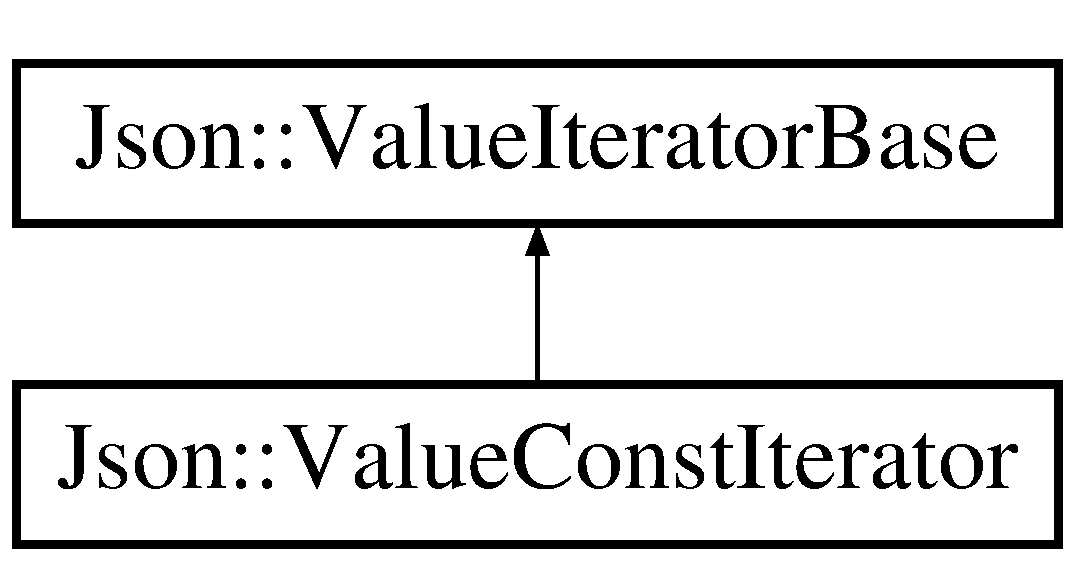
\includegraphics[height=2.000000cm]{class_json_1_1_value_const_iterator}
\end{center}
\end{figure}
\subsection*{Public Types}
\begin{DoxyCompactItemize}
\item 
typedef const \hyperlink{class_json_1_1_value}{Value} \hyperlink{class_json_1_1_value_const_iterator_aa5f1707dcef4bfe73e23ddc14dbe760d}{value\-\_\-type}
\item 
typedef unsigned int \hyperlink{class_json_1_1_value_const_iterator_a8685219d214dbd2b763357ae94fb0f27}{size\-\_\-t}
\item 
typedef int \hyperlink{class_json_1_1_value_const_iterator_a32b36aa9d76e2b48ca74fb6e1979a95a}{difference\-\_\-type}
\item 
typedef const \hyperlink{class_json_1_1_value}{Value} \& \hyperlink{class_json_1_1_value_const_iterator_aa9b05c6a37cd352ea1ee6e13b816f709}{reference}
\item 
typedef const \hyperlink{class_json_1_1_value}{Value} $\ast$ \hyperlink{class_json_1_1_value_const_iterator_a400136bd8bc09e9fddec0785fa2cff14}{pointer}
\item 
typedef \hyperlink{class_json_1_1_value_const_iterator}{Value\-Const\-Iterator} \hyperlink{class_json_1_1_value_const_iterator_a0c2e33e7eb5a80dd8709fb28ece83933}{Self\-Type}
\end{DoxyCompactItemize}
\subsection*{Public Member Functions}
\begin{DoxyCompactItemize}
\item 
\hyperlink{class_json_1_1_value_const_iterator_a1b10a46f1606421b0663492a5f9a2aad}{Value\-Const\-Iterator} ()
\item 
\hyperlink{class_json_1_1_value_iterator_base_a9d2a940d03ea06d20d972f41a89149ee}{Self\-Type} \& \hyperlink{class_json_1_1_value_const_iterator_ad1b1c11f8d7fb22d4d3c231915f2b15b}{operator=} (const \hyperlink{class_json_1_1_value_iterator_base}{Value\-Iterator\-Base} \&other)
\item 
\hyperlink{class_json_1_1_value_iterator_base_a9d2a940d03ea06d20d972f41a89149ee}{Self\-Type} \hyperlink{class_json_1_1_value_const_iterator_ab3f0c2edbfc8f7d60645f3d597d05e28}{operator++} (int)
\item 
\hyperlink{class_json_1_1_value_iterator_base_a9d2a940d03ea06d20d972f41a89149ee}{Self\-Type} \hyperlink{class_json_1_1_value_const_iterator_a94935961e9331c6f7b907b05ec8df75e}{operator-\/-\/} (int)
\item 
\hyperlink{class_json_1_1_value_iterator_base_a9d2a940d03ea06d20d972f41a89149ee}{Self\-Type} \& \hyperlink{class_json_1_1_value_const_iterator_a31415e44e44e56fb2bfda7e8bb784646}{operator-\/-\/} ()
\item 
\hyperlink{class_json_1_1_value_iterator_base_a9d2a940d03ea06d20d972f41a89149ee}{Self\-Type} \& \hyperlink{class_json_1_1_value_const_iterator_a2cfe2f7a94a688186efdafb1b181c319}{operator++} ()
\item 
\hyperlink{class_json_1_1_value_const_iterator_aa9b05c6a37cd352ea1ee6e13b816f709}{reference} \hyperlink{class_json_1_1_value_const_iterator_aeb44153d71c61ac9397a84d5ecc244c5}{operator$\ast$} () const 
\item 
\hyperlink{class_json_1_1_value_const_iterator_a400136bd8bc09e9fddec0785fa2cff14}{pointer} \hyperlink{class_json_1_1_value_const_iterator_ac493d31c8eede8af10b71415fe8e624b}{operator-\/$>$} () const 
\end{DoxyCompactItemize}
\subsection*{Friends}
\begin{DoxyCompactItemize}
\item 
class \hyperlink{class_json_1_1_value_const_iterator_aeceedf6e1a7d48a588516ce2b1983d6f}{Value}
\end{DoxyCompactItemize}
\subsection*{Additional Inherited Members}


\subsection{Detailed Description}
const iterator for object and array value. 



Definition at line 1340 of file json.\-hpp.



\subsection{Member Typedef Documentation}
\hypertarget{class_json_1_1_value_const_iterator_a32b36aa9d76e2b48ca74fb6e1979a95a}{\index{Json\-::\-Value\-Const\-Iterator@{Json\-::\-Value\-Const\-Iterator}!difference\-\_\-type@{difference\-\_\-type}}
\index{difference\-\_\-type@{difference\-\_\-type}!Json::ValueConstIterator@{Json\-::\-Value\-Const\-Iterator}}
\subsubsection[{difference\-\_\-type}]{\setlength{\rightskip}{0pt plus 5cm}typedef int {\bf Json\-::\-Value\-Const\-Iterator\-::difference\-\_\-type}}}\label{class_json_1_1_value_const_iterator_a32b36aa9d76e2b48ca74fb6e1979a95a}


Definition at line 1346 of file json.\-hpp.

\hypertarget{class_json_1_1_value_const_iterator_a400136bd8bc09e9fddec0785fa2cff14}{\index{Json\-::\-Value\-Const\-Iterator@{Json\-::\-Value\-Const\-Iterator}!pointer@{pointer}}
\index{pointer@{pointer}!Json::ValueConstIterator@{Json\-::\-Value\-Const\-Iterator}}
\subsubsection[{pointer}]{\setlength{\rightskip}{0pt plus 5cm}typedef const {\bf Value}$\ast$ {\bf Json\-::\-Value\-Const\-Iterator\-::pointer}}}\label{class_json_1_1_value_const_iterator_a400136bd8bc09e9fddec0785fa2cff14}


Definition at line 1348 of file json.\-hpp.

\hypertarget{class_json_1_1_value_const_iterator_aa9b05c6a37cd352ea1ee6e13b816f709}{\index{Json\-::\-Value\-Const\-Iterator@{Json\-::\-Value\-Const\-Iterator}!reference@{reference}}
\index{reference@{reference}!Json::ValueConstIterator@{Json\-::\-Value\-Const\-Iterator}}
\subsubsection[{reference}]{\setlength{\rightskip}{0pt plus 5cm}typedef const {\bf Value}\& {\bf Json\-::\-Value\-Const\-Iterator\-::reference}}}\label{class_json_1_1_value_const_iterator_aa9b05c6a37cd352ea1ee6e13b816f709}


Definition at line 1347 of file json.\-hpp.

\hypertarget{class_json_1_1_value_const_iterator_a0c2e33e7eb5a80dd8709fb28ece83933}{\index{Json\-::\-Value\-Const\-Iterator@{Json\-::\-Value\-Const\-Iterator}!Self\-Type@{Self\-Type}}
\index{Self\-Type@{Self\-Type}!Json::ValueConstIterator@{Json\-::\-Value\-Const\-Iterator}}
\subsubsection[{Self\-Type}]{\setlength{\rightskip}{0pt plus 5cm}typedef {\bf Value\-Const\-Iterator} {\bf Json\-::\-Value\-Const\-Iterator\-::\-Self\-Type}}}\label{class_json_1_1_value_const_iterator_a0c2e33e7eb5a80dd8709fb28ece83933}


Definition at line 1349 of file json.\-hpp.

\hypertarget{class_json_1_1_value_const_iterator_a8685219d214dbd2b763357ae94fb0f27}{\index{Json\-::\-Value\-Const\-Iterator@{Json\-::\-Value\-Const\-Iterator}!size\-\_\-t@{size\-\_\-t}}
\index{size\-\_\-t@{size\-\_\-t}!Json::ValueConstIterator@{Json\-::\-Value\-Const\-Iterator}}
\subsubsection[{size\-\_\-t}]{\setlength{\rightskip}{0pt plus 5cm}typedef unsigned int {\bf Json\-::\-Value\-Const\-Iterator\-::size\-\_\-t}}}\label{class_json_1_1_value_const_iterator_a8685219d214dbd2b763357ae94fb0f27}


Definition at line 1345 of file json.\-hpp.

\hypertarget{class_json_1_1_value_const_iterator_aa5f1707dcef4bfe73e23ddc14dbe760d}{\index{Json\-::\-Value\-Const\-Iterator@{Json\-::\-Value\-Const\-Iterator}!value\-\_\-type@{value\-\_\-type}}
\index{value\-\_\-type@{value\-\_\-type}!Json::ValueConstIterator@{Json\-::\-Value\-Const\-Iterator}}
\subsubsection[{value\-\_\-type}]{\setlength{\rightskip}{0pt plus 5cm}typedef const {\bf Value} {\bf Json\-::\-Value\-Const\-Iterator\-::value\-\_\-type}}}\label{class_json_1_1_value_const_iterator_aa5f1707dcef4bfe73e23ddc14dbe760d}


Definition at line 1344 of file json.\-hpp.



\subsection{Constructor \& Destructor Documentation}
\hypertarget{class_json_1_1_value_const_iterator_a1b10a46f1606421b0663492a5f9a2aad}{\index{Json\-::\-Value\-Const\-Iterator@{Json\-::\-Value\-Const\-Iterator}!Value\-Const\-Iterator@{Value\-Const\-Iterator}}
\index{Value\-Const\-Iterator@{Value\-Const\-Iterator}!Json::ValueConstIterator@{Json\-::\-Value\-Const\-Iterator}}
\subsubsection[{Value\-Const\-Iterator}]{\setlength{\rightskip}{0pt plus 5cm}Json\-::\-Value\-Const\-Iterator\-::\-Value\-Const\-Iterator (
\begin{DoxyParamCaption}
{}
\end{DoxyParamCaption}
)}}\label{class_json_1_1_value_const_iterator_a1b10a46f1606421b0663492a5f9a2aad}


Definition at line 1404 of file json.\-cpp.



\subsection{Member Function Documentation}
\hypertarget{class_json_1_1_value_const_iterator_aeb44153d71c61ac9397a84d5ecc244c5}{\index{Json\-::\-Value\-Const\-Iterator@{Json\-::\-Value\-Const\-Iterator}!operator$\ast$@{operator$\ast$}}
\index{operator$\ast$@{operator$\ast$}!Json::ValueConstIterator@{Json\-::\-Value\-Const\-Iterator}}
\subsubsection[{operator$\ast$}]{\setlength{\rightskip}{0pt plus 5cm}{\bf reference} Json\-::\-Value\-Const\-Iterator\-::operator$\ast$ (
\begin{DoxyParamCaption}
{}
\end{DoxyParamCaption}
) const\hspace{0.3cm}{\ttfamily [inline]}}}\label{class_json_1_1_value_const_iterator_aeb44153d71c61ac9397a84d5ecc244c5}


Definition at line 1387 of file json.\-hpp.

\hypertarget{class_json_1_1_value_const_iterator_ab3f0c2edbfc8f7d60645f3d597d05e28}{\index{Json\-::\-Value\-Const\-Iterator@{Json\-::\-Value\-Const\-Iterator}!operator++@{operator++}}
\index{operator++@{operator++}!Json::ValueConstIterator@{Json\-::\-Value\-Const\-Iterator}}
\subsubsection[{operator++}]{\setlength{\rightskip}{0pt plus 5cm}{\bf Self\-Type} Json\-::\-Value\-Const\-Iterator\-::operator++ (
\begin{DoxyParamCaption}
\item[{int}]{}
\end{DoxyParamCaption}
)\hspace{0.3cm}{\ttfamily [inline]}}}\label{class_json_1_1_value_const_iterator_ab3f0c2edbfc8f7d60645f3d597d05e28}


Definition at line 1365 of file json.\-hpp.

\hypertarget{class_json_1_1_value_const_iterator_a2cfe2f7a94a688186efdafb1b181c319}{\index{Json\-::\-Value\-Const\-Iterator@{Json\-::\-Value\-Const\-Iterator}!operator++@{operator++}}
\index{operator++@{operator++}!Json::ValueConstIterator@{Json\-::\-Value\-Const\-Iterator}}
\subsubsection[{operator++}]{\setlength{\rightskip}{0pt plus 5cm}{\bf Self\-Type}\& Json\-::\-Value\-Const\-Iterator\-::operator++ (
\begin{DoxyParamCaption}
{}
\end{DoxyParamCaption}
)\hspace{0.3cm}{\ttfamily [inline]}}}\label{class_json_1_1_value_const_iterator_a2cfe2f7a94a688186efdafb1b181c319}


Definition at line 1382 of file json.\-hpp.

\hypertarget{class_json_1_1_value_const_iterator_a94935961e9331c6f7b907b05ec8df75e}{\index{Json\-::\-Value\-Const\-Iterator@{Json\-::\-Value\-Const\-Iterator}!operator-\/-\/@{operator-\/-\/}}
\index{operator-\/-\/@{operator-\/-\/}!Json::ValueConstIterator@{Json\-::\-Value\-Const\-Iterator}}
\subsubsection[{operator-\/-\/}]{\setlength{\rightskip}{0pt plus 5cm}{\bf Self\-Type} Json\-::\-Value\-Const\-Iterator\-::operator-\/-\/ (
\begin{DoxyParamCaption}
\item[{int}]{}
\end{DoxyParamCaption}
)\hspace{0.3cm}{\ttfamily [inline]}}}\label{class_json_1_1_value_const_iterator_a94935961e9331c6f7b907b05ec8df75e}


Definition at line 1371 of file json.\-hpp.

\hypertarget{class_json_1_1_value_const_iterator_a31415e44e44e56fb2bfda7e8bb784646}{\index{Json\-::\-Value\-Const\-Iterator@{Json\-::\-Value\-Const\-Iterator}!operator-\/-\/@{operator-\/-\/}}
\index{operator-\/-\/@{operator-\/-\/}!Json::ValueConstIterator@{Json\-::\-Value\-Const\-Iterator}}
\subsubsection[{operator-\/-\/}]{\setlength{\rightskip}{0pt plus 5cm}{\bf Self\-Type}\& Json\-::\-Value\-Const\-Iterator\-::operator-\/-\/ (
\begin{DoxyParamCaption}
{}
\end{DoxyParamCaption}
)\hspace{0.3cm}{\ttfamily [inline]}}}\label{class_json_1_1_value_const_iterator_a31415e44e44e56fb2bfda7e8bb784646}


Definition at line 1377 of file json.\-hpp.

\hypertarget{class_json_1_1_value_const_iterator_ac493d31c8eede8af10b71415fe8e624b}{\index{Json\-::\-Value\-Const\-Iterator@{Json\-::\-Value\-Const\-Iterator}!operator-\/$>$@{operator-\/$>$}}
\index{operator-\/$>$@{operator-\/$>$}!Json::ValueConstIterator@{Json\-::\-Value\-Const\-Iterator}}
\subsubsection[{operator-\/$>$}]{\setlength{\rightskip}{0pt plus 5cm}{\bf pointer} Json\-::\-Value\-Const\-Iterator\-::operator-\/$>$ (
\begin{DoxyParamCaption}
{}
\end{DoxyParamCaption}
) const\hspace{0.3cm}{\ttfamily [inline]}}}\label{class_json_1_1_value_const_iterator_ac493d31c8eede8af10b71415fe8e624b}


Definition at line 1389 of file json.\-hpp.

\hypertarget{class_json_1_1_value_const_iterator_ad1b1c11f8d7fb22d4d3c231915f2b15b}{\index{Json\-::\-Value\-Const\-Iterator@{Json\-::\-Value\-Const\-Iterator}!operator=@{operator=}}
\index{operator=@{operator=}!Json::ValueConstIterator@{Json\-::\-Value\-Const\-Iterator}}
\subsubsection[{operator=}]{\setlength{\rightskip}{0pt plus 5cm}{\bf Value\-Const\-Iterator} \& Json\-::\-Value\-Const\-Iterator\-::operator= (
\begin{DoxyParamCaption}
\item[{const {\bf Value\-Iterator\-Base} \&}]{other}
\end{DoxyParamCaption}
)}}\label{class_json_1_1_value_const_iterator_ad1b1c11f8d7fb22d4d3c231915f2b15b}


Definition at line 1421 of file json.\-cpp.



\subsection{Friends And Related Function Documentation}
\hypertarget{class_json_1_1_value_const_iterator_aeceedf6e1a7d48a588516ce2b1983d6f}{\index{Json\-::\-Value\-Const\-Iterator@{Json\-::\-Value\-Const\-Iterator}!Value@{Value}}
\index{Value@{Value}!Json::ValueConstIterator@{Json\-::\-Value\-Const\-Iterator}}
\subsubsection[{Value}]{\setlength{\rightskip}{0pt plus 5cm}friend class {\bf Value}\hspace{0.3cm}{\ttfamily [friend]}}}\label{class_json_1_1_value_const_iterator_aeceedf6e1a7d48a588516ce2b1983d6f}


Definition at line 1341 of file json.\-hpp.



The documentation for this class was generated from the following files\-:\begin{DoxyCompactItemize}
\item 
/home/fushigisama/\-Documents/amon/includes/util/json/\hyperlink{json_8hpp}{json.\-hpp}\item 
/home/fushigisama/\-Documents/amon/src/util/json/\hyperlink{json_8cpp}{json.\-cpp}\end{DoxyCompactItemize}

\hypertarget{class_json_1_1_value_iterator}{\section{Json\-:\-:Value\-Iterator Class Reference}
\label{class_json_1_1_value_iterator}\index{Json\-::\-Value\-Iterator@{Json\-::\-Value\-Iterator}}
}


Iterator for object and array value.  




{\ttfamily \#include $<$json.\-hpp$>$}

Inheritance diagram for Json\-:\-:Value\-Iterator\-:\begin{figure}[H]
\begin{center}
\leavevmode
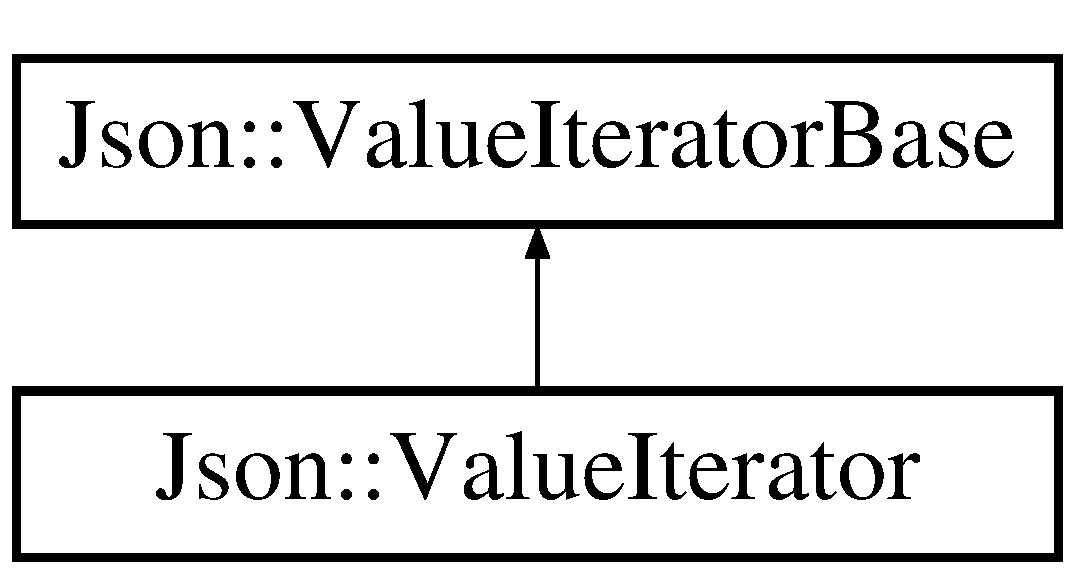
\includegraphics[height=2.000000cm]{class_json_1_1_value_iterator}
\end{center}
\end{figure}
\subsection*{Public Types}
\begin{DoxyCompactItemize}
\item 
typedef \hyperlink{class_json_1_1_value}{Value} \hyperlink{class_json_1_1_value_iterator_a2c5ba7be611f05546530c8a88b2d2e37}{value\-\_\-type}
\item 
typedef unsigned int \hyperlink{class_json_1_1_value_iterator_a308b8932ffc83eaa9d12dadd5c11a7dd}{size\-\_\-t}
\item 
typedef int \hyperlink{class_json_1_1_value_iterator_a2be1a9aa60bbfc8812e9dd1a7f1a8786}{difference\-\_\-type}
\item 
typedef \hyperlink{class_json_1_1_value}{Value} \& \hyperlink{class_json_1_1_value_iterator_ae87929b4567aa00372cf602c43b57160}{reference}
\item 
typedef \hyperlink{class_json_1_1_value}{Value} $\ast$ \hyperlink{class_json_1_1_value_iterator_acec45feb1ef1f3bf81240157d06d5432}{pointer}
\item 
typedef \hyperlink{class_json_1_1_value_iterator}{Value\-Iterator} \hyperlink{class_json_1_1_value_iterator_a23357670fdad61792670d86f62db7e16}{Self\-Type}
\end{DoxyCompactItemize}
\subsection*{Public Member Functions}
\begin{DoxyCompactItemize}
\item 
\hyperlink{class_json_1_1_value_iterator_a09425cf4dc12244072a942f290a5c0ec}{Value\-Iterator} ()
\item 
\hyperlink{class_json_1_1_value_iterator_aa85aa208670891670392259efa0143bb}{Value\-Iterator} (const \hyperlink{class_json_1_1_value_const_iterator}{Value\-Const\-Iterator} \&other)
\item 
\hyperlink{class_json_1_1_value_iterator_a7d5e58a9a4a553968acdf3064b39d21c}{Value\-Iterator} (const \hyperlink{class_json_1_1_value_iterator}{Value\-Iterator} \&other)
\item 
\hyperlink{class_json_1_1_value_iterator_base_a9d2a940d03ea06d20d972f41a89149ee}{Self\-Type} \& \hyperlink{class_json_1_1_value_iterator_a8e23312b1db874f7e403fd7e76611bdc}{operator=} (const \hyperlink{class_json_1_1_value_iterator_base_a9d2a940d03ea06d20d972f41a89149ee}{Self\-Type} \&other)
\item 
\hyperlink{class_json_1_1_value_iterator_base_a9d2a940d03ea06d20d972f41a89149ee}{Self\-Type} \hyperlink{class_json_1_1_value_iterator_abcf4ddd994a010742cd4a436d65acd08}{operator++} (int)
\item 
\hyperlink{class_json_1_1_value_iterator_base_a9d2a940d03ea06d20d972f41a89149ee}{Self\-Type} \hyperlink{class_json_1_1_value_iterator_a06d6a29d96caf6af324a53973159e12b}{operator-\/-\/} (int)
\item 
\hyperlink{class_json_1_1_value_iterator_base_a9d2a940d03ea06d20d972f41a89149ee}{Self\-Type} \& \hyperlink{class_json_1_1_value_iterator_a811302a868518a0995a9def955df5720}{operator-\/-\/} ()
\item 
\hyperlink{class_json_1_1_value_iterator_base_a9d2a940d03ea06d20d972f41a89149ee}{Self\-Type} \& \hyperlink{class_json_1_1_value_iterator_a92146c46f8249e2b2d12869e70cd4cee}{operator++} ()
\item 
\hyperlink{class_json_1_1_value_iterator_ae87929b4567aa00372cf602c43b57160}{reference} \hyperlink{class_json_1_1_value_iterator_aaa5be3457eedf0526a03b8a3b4c7c0a0}{operator$\ast$} () const 
\item 
\hyperlink{class_json_1_1_value_iterator_acec45feb1ef1f3bf81240157d06d5432}{pointer} \hyperlink{class_json_1_1_value_iterator_ad9882e4ce815cef6a504afa113544bfb}{operator-\/$>$} () const 
\end{DoxyCompactItemize}
\subsection*{Friends}
\begin{DoxyCompactItemize}
\item 
class \hyperlink{class_json_1_1_value_iterator_aeceedf6e1a7d48a588516ce2b1983d6f}{Value}
\end{DoxyCompactItemize}
\subsection*{Additional Inherited Members}


\subsection{Detailed Description}
Iterator for object and array value. 

Definition at line 1394 of file json.\-hpp.



\subsection{Member Typedef Documentation}
\hypertarget{class_json_1_1_value_iterator_a2be1a9aa60bbfc8812e9dd1a7f1a8786}{\index{Json\-::\-Value\-Iterator@{Json\-::\-Value\-Iterator}!difference\-\_\-type@{difference\-\_\-type}}
\index{difference\-\_\-type@{difference\-\_\-type}!Json::ValueIterator@{Json\-::\-Value\-Iterator}}
\subsubsection[{difference\-\_\-type}]{\setlength{\rightskip}{0pt plus 5cm}typedef int {\bf Json\-::\-Value\-Iterator\-::difference\-\_\-type}}}\label{class_json_1_1_value_iterator_a2be1a9aa60bbfc8812e9dd1a7f1a8786}


Definition at line 1400 of file json.\-hpp.

\hypertarget{class_json_1_1_value_iterator_acec45feb1ef1f3bf81240157d06d5432}{\index{Json\-::\-Value\-Iterator@{Json\-::\-Value\-Iterator}!pointer@{pointer}}
\index{pointer@{pointer}!Json::ValueIterator@{Json\-::\-Value\-Iterator}}
\subsubsection[{pointer}]{\setlength{\rightskip}{0pt plus 5cm}typedef {\bf Value}$\ast$ {\bf Json\-::\-Value\-Iterator\-::pointer}}}\label{class_json_1_1_value_iterator_acec45feb1ef1f3bf81240157d06d5432}


Definition at line 1402 of file json.\-hpp.

\hypertarget{class_json_1_1_value_iterator_ae87929b4567aa00372cf602c43b57160}{\index{Json\-::\-Value\-Iterator@{Json\-::\-Value\-Iterator}!reference@{reference}}
\index{reference@{reference}!Json::ValueIterator@{Json\-::\-Value\-Iterator}}
\subsubsection[{reference}]{\setlength{\rightskip}{0pt plus 5cm}typedef {\bf Value}\& {\bf Json\-::\-Value\-Iterator\-::reference}}}\label{class_json_1_1_value_iterator_ae87929b4567aa00372cf602c43b57160}


Definition at line 1401 of file json.\-hpp.

\hypertarget{class_json_1_1_value_iterator_a23357670fdad61792670d86f62db7e16}{\index{Json\-::\-Value\-Iterator@{Json\-::\-Value\-Iterator}!Self\-Type@{Self\-Type}}
\index{Self\-Type@{Self\-Type}!Json::ValueIterator@{Json\-::\-Value\-Iterator}}
\subsubsection[{Self\-Type}]{\setlength{\rightskip}{0pt plus 5cm}typedef {\bf Value\-Iterator} {\bf Json\-::\-Value\-Iterator\-::\-Self\-Type}}}\label{class_json_1_1_value_iterator_a23357670fdad61792670d86f62db7e16}


Definition at line 1403 of file json.\-hpp.

\hypertarget{class_json_1_1_value_iterator_a308b8932ffc83eaa9d12dadd5c11a7dd}{\index{Json\-::\-Value\-Iterator@{Json\-::\-Value\-Iterator}!size\-\_\-t@{size\-\_\-t}}
\index{size\-\_\-t@{size\-\_\-t}!Json::ValueIterator@{Json\-::\-Value\-Iterator}}
\subsubsection[{size\-\_\-t}]{\setlength{\rightskip}{0pt plus 5cm}typedef unsigned int {\bf Json\-::\-Value\-Iterator\-::size\-\_\-t}}}\label{class_json_1_1_value_iterator_a308b8932ffc83eaa9d12dadd5c11a7dd}


Definition at line 1399 of file json.\-hpp.

\hypertarget{class_json_1_1_value_iterator_a2c5ba7be611f05546530c8a88b2d2e37}{\index{Json\-::\-Value\-Iterator@{Json\-::\-Value\-Iterator}!value\-\_\-type@{value\-\_\-type}}
\index{value\-\_\-type@{value\-\_\-type}!Json::ValueIterator@{Json\-::\-Value\-Iterator}}
\subsubsection[{value\-\_\-type}]{\setlength{\rightskip}{0pt plus 5cm}typedef {\bf Value} {\bf Json\-::\-Value\-Iterator\-::value\-\_\-type}}}\label{class_json_1_1_value_iterator_a2c5ba7be611f05546530c8a88b2d2e37}


Definition at line 1398 of file json.\-hpp.



\subsection{Constructor \& Destructor Documentation}
\hypertarget{class_json_1_1_value_iterator_a09425cf4dc12244072a942f290a5c0ec}{\index{Json\-::\-Value\-Iterator@{Json\-::\-Value\-Iterator}!Value\-Iterator@{Value\-Iterator}}
\index{Value\-Iterator@{Value\-Iterator}!Json::ValueIterator@{Json\-::\-Value\-Iterator}}
\subsubsection[{Value\-Iterator}]{\setlength{\rightskip}{0pt plus 5cm}Json\-::\-Value\-Iterator\-::\-Value\-Iterator (
\begin{DoxyParamCaption}
{}
\end{DoxyParamCaption}
)}}\label{class_json_1_1_value_iterator_a09425cf4dc12244072a942f290a5c0ec}


Definition at line 1434 of file json.\-cpp.

\hypertarget{class_json_1_1_value_iterator_aa85aa208670891670392259efa0143bb}{\index{Json\-::\-Value\-Iterator@{Json\-::\-Value\-Iterator}!Value\-Iterator@{Value\-Iterator}}
\index{Value\-Iterator@{Value\-Iterator}!Json::ValueIterator@{Json\-::\-Value\-Iterator}}
\subsubsection[{Value\-Iterator}]{\setlength{\rightskip}{0pt plus 5cm}Json\-::\-Value\-Iterator\-::\-Value\-Iterator (
\begin{DoxyParamCaption}
\item[{const {\bf Value\-Const\-Iterator} \&}]{other}
\end{DoxyParamCaption}
)}}\label{class_json_1_1_value_iterator_aa85aa208670891670392259efa0143bb}


Definition at line 1447 of file json.\-cpp.

\hypertarget{class_json_1_1_value_iterator_a7d5e58a9a4a553968acdf3064b39d21c}{\index{Json\-::\-Value\-Iterator@{Json\-::\-Value\-Iterator}!Value\-Iterator@{Value\-Iterator}}
\index{Value\-Iterator@{Value\-Iterator}!Json::ValueIterator@{Json\-::\-Value\-Iterator}}
\subsubsection[{Value\-Iterator}]{\setlength{\rightskip}{0pt plus 5cm}Json\-::\-Value\-Iterator\-::\-Value\-Iterator (
\begin{DoxyParamCaption}
\item[{const {\bf Value\-Iterator} \&}]{other}
\end{DoxyParamCaption}
)}}\label{class_json_1_1_value_iterator_a7d5e58a9a4a553968acdf3064b39d21c}


Definition at line 1450 of file json.\-cpp.



\subsection{Member Function Documentation}
\hypertarget{class_json_1_1_value_iterator_aaa5be3457eedf0526a03b8a3b4c7c0a0}{\index{Json\-::\-Value\-Iterator@{Json\-::\-Value\-Iterator}!operator$\ast$@{operator$\ast$}}
\index{operator$\ast$@{operator$\ast$}!Json::ValueIterator@{Json\-::\-Value\-Iterator}}
\subsubsection[{operator$\ast$}]{\setlength{\rightskip}{0pt plus 5cm}{\bf reference} Json\-::\-Value\-Iterator\-::operator$\ast$ (
\begin{DoxyParamCaption}
{}
\end{DoxyParamCaption}
) const\hspace{0.3cm}{\ttfamily [inline]}}}\label{class_json_1_1_value_iterator_aaa5be3457eedf0526a03b8a3b4c7c0a0}


Definition at line 1443 of file json.\-hpp.

\hypertarget{class_json_1_1_value_iterator_abcf4ddd994a010742cd4a436d65acd08}{\index{Json\-::\-Value\-Iterator@{Json\-::\-Value\-Iterator}!operator++@{operator++}}
\index{operator++@{operator++}!Json::ValueIterator@{Json\-::\-Value\-Iterator}}
\subsubsection[{operator++}]{\setlength{\rightskip}{0pt plus 5cm}{\bf Self\-Type} Json\-::\-Value\-Iterator\-::operator++ (
\begin{DoxyParamCaption}
\item[{int}]{}
\end{DoxyParamCaption}
)\hspace{0.3cm}{\ttfamily [inline]}}}\label{class_json_1_1_value_iterator_abcf4ddd994a010742cd4a436d65acd08}


Definition at line 1421 of file json.\-hpp.

\hypertarget{class_json_1_1_value_iterator_a92146c46f8249e2b2d12869e70cd4cee}{\index{Json\-::\-Value\-Iterator@{Json\-::\-Value\-Iterator}!operator++@{operator++}}
\index{operator++@{operator++}!Json::ValueIterator@{Json\-::\-Value\-Iterator}}
\subsubsection[{operator++}]{\setlength{\rightskip}{0pt plus 5cm}{\bf Self\-Type}\& Json\-::\-Value\-Iterator\-::operator++ (
\begin{DoxyParamCaption}
{}
\end{DoxyParamCaption}
)\hspace{0.3cm}{\ttfamily [inline]}}}\label{class_json_1_1_value_iterator_a92146c46f8249e2b2d12869e70cd4cee}


Definition at line 1438 of file json.\-hpp.

\hypertarget{class_json_1_1_value_iterator_a06d6a29d96caf6af324a53973159e12b}{\index{Json\-::\-Value\-Iterator@{Json\-::\-Value\-Iterator}!operator-\/-\/@{operator-\/-\/}}
\index{operator-\/-\/@{operator-\/-\/}!Json::ValueIterator@{Json\-::\-Value\-Iterator}}
\subsubsection[{operator-\/-\/}]{\setlength{\rightskip}{0pt plus 5cm}{\bf Self\-Type} Json\-::\-Value\-Iterator\-::operator-\/-\/ (
\begin{DoxyParamCaption}
\item[{int}]{}
\end{DoxyParamCaption}
)\hspace{0.3cm}{\ttfamily [inline]}}}\label{class_json_1_1_value_iterator_a06d6a29d96caf6af324a53973159e12b}


Definition at line 1427 of file json.\-hpp.

\hypertarget{class_json_1_1_value_iterator_a811302a868518a0995a9def955df5720}{\index{Json\-::\-Value\-Iterator@{Json\-::\-Value\-Iterator}!operator-\/-\/@{operator-\/-\/}}
\index{operator-\/-\/@{operator-\/-\/}!Json::ValueIterator@{Json\-::\-Value\-Iterator}}
\subsubsection[{operator-\/-\/}]{\setlength{\rightskip}{0pt plus 5cm}{\bf Self\-Type}\& Json\-::\-Value\-Iterator\-::operator-\/-\/ (
\begin{DoxyParamCaption}
{}
\end{DoxyParamCaption}
)\hspace{0.3cm}{\ttfamily [inline]}}}\label{class_json_1_1_value_iterator_a811302a868518a0995a9def955df5720}


Definition at line 1433 of file json.\-hpp.

\hypertarget{class_json_1_1_value_iterator_ad9882e4ce815cef6a504afa113544bfb}{\index{Json\-::\-Value\-Iterator@{Json\-::\-Value\-Iterator}!operator-\/$>$@{operator-\/$>$}}
\index{operator-\/$>$@{operator-\/$>$}!Json::ValueIterator@{Json\-::\-Value\-Iterator}}
\subsubsection[{operator-\/$>$}]{\setlength{\rightskip}{0pt plus 5cm}{\bf pointer} Json\-::\-Value\-Iterator\-::operator-\/$>$ (
\begin{DoxyParamCaption}
{}
\end{DoxyParamCaption}
) const\hspace{0.3cm}{\ttfamily [inline]}}}\label{class_json_1_1_value_iterator_ad9882e4ce815cef6a504afa113544bfb}


Definition at line 1445 of file json.\-hpp.

\hypertarget{class_json_1_1_value_iterator_a8e23312b1db874f7e403fd7e76611bdc}{\index{Json\-::\-Value\-Iterator@{Json\-::\-Value\-Iterator}!operator=@{operator=}}
\index{operator=@{operator=}!Json::ValueIterator@{Json\-::\-Value\-Iterator}}
\subsubsection[{operator=}]{\setlength{\rightskip}{0pt plus 5cm}{\bf Value\-Iterator} \& Json\-::\-Value\-Iterator\-::operator= (
\begin{DoxyParamCaption}
\item[{const {\bf Self\-Type} \&}]{other}
\end{DoxyParamCaption}
)}}\label{class_json_1_1_value_iterator_a8e23312b1db874f7e403fd7e76611bdc}


Definition at line 1453 of file json.\-cpp.



\subsection{Friends And Related Function Documentation}
\hypertarget{class_json_1_1_value_iterator_aeceedf6e1a7d48a588516ce2b1983d6f}{\index{Json\-::\-Value\-Iterator@{Json\-::\-Value\-Iterator}!Value@{Value}}
\index{Value@{Value}!Json::ValueIterator@{Json\-::\-Value\-Iterator}}
\subsubsection[{Value}]{\setlength{\rightskip}{0pt plus 5cm}friend class {\bf Value}\hspace{0.3cm}{\ttfamily [friend]}}}\label{class_json_1_1_value_iterator_aeceedf6e1a7d48a588516ce2b1983d6f}


Definition at line 1395 of file json.\-hpp.



The documentation for this class was generated from the following files\-:\begin{DoxyCompactItemize}
\item 
/home/fushigisama/\-Documents/amon/includes/util/json/\hyperlink{json_8hpp}{json.\-hpp}\item 
/home/fushigisama/\-Documents/amon/src/util/json/\hyperlink{json_8cpp}{json.\-cpp}\end{DoxyCompactItemize}

\hypertarget{class_json_1_1_value_iterator_base}{\section{Json\-:\-:Value\-Iterator\-Base Class Reference}
\label{class_json_1_1_value_iterator_base}\index{Json\-::\-Value\-Iterator\-Base@{Json\-::\-Value\-Iterator\-Base}}
}


base class for \hyperlink{class_json_1_1_value}{Value} iterators.  




{\ttfamily \#include $<$json.\-hpp$>$}

Inheritance diagram for Json\-:\-:Value\-Iterator\-Base\-:\begin{figure}[H]
\begin{center}
\leavevmode
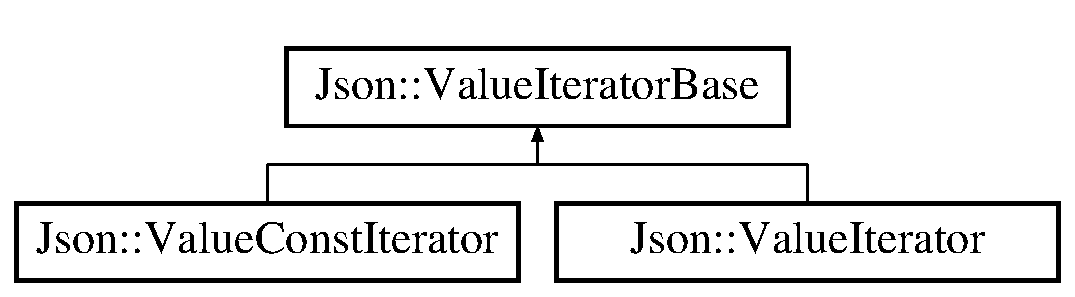
\includegraphics[height=2.000000cm]{class_json_1_1_value_iterator_base}
\end{center}
\end{figure}
\subsection*{Public Types}
\begin{DoxyCompactItemize}
\item 
typedef \\*
std\-::bidirectional\-\_\-iterator\-\_\-tag \hyperlink{class_json_1_1_value_iterator_base_a02fd11a4fbdc0007da1e8bcf5e6b83c3}{iterator\-\_\-category}
\item 
typedef unsigned int \hyperlink{class_json_1_1_value_iterator_base_a9d3a3c7ce5cdefe23cb486239cf07bb5}{size\-\_\-t}
\item 
typedef int \hyperlink{class_json_1_1_value_iterator_base_a4e44bf8cbd17ec8d6e2c185904a15ebd}{difference\-\_\-type}
\item 
typedef \hyperlink{class_json_1_1_value_iterator_base}{Value\-Iterator\-Base} \hyperlink{class_json_1_1_value_iterator_base_a9d2a940d03ea06d20d972f41a89149ee}{Self\-Type}
\end{DoxyCompactItemize}
\subsection*{Public Member Functions}
\begin{DoxyCompactItemize}
\item 
\hyperlink{class_json_1_1_value_iterator_base_af45b028d9ff9cbd2554a87878b42dd75}{Value\-Iterator\-Base} ()
\item 
\hyperlink{class_json_1_1_value_iterator_base_a640e990e5f03a96fd650122a2906f59d}{Value\-Iterator\-Base} (const Value\-::\-Object\-Values\-::iterator \&current)
\item 
bool \hyperlink{class_json_1_1_value_iterator_base_afc656672ac28502f640ade32c38c1b56}{operator==} (const \hyperlink{class_json_1_1_value_iterator_base_a9d2a940d03ea06d20d972f41a89149ee}{Self\-Type} \&other) const 
\item 
bool \hyperlink{class_json_1_1_value_iterator_base_a18c2dd42e0bb989ace141bfe9de52792}{operator!=} (const \hyperlink{class_json_1_1_value_iterator_base_a9d2a940d03ea06d20d972f41a89149ee}{Self\-Type} \&other) const 
\item 
\hyperlink{class_json_1_1_value_iterator_base_a4e44bf8cbd17ec8d6e2c185904a15ebd}{difference\-\_\-type} \hyperlink{class_json_1_1_value_iterator_base_ab786787fcad68ca5e8745aaf520fa17f}{operator-\/} (const \hyperlink{class_json_1_1_value_iterator_base_a9d2a940d03ea06d20d972f41a89149ee}{Self\-Type} \&other) const 
\item 
\hyperlink{class_json_1_1_value}{Value} \hyperlink{class_json_1_1_value_iterator_base_aa2ff5e79fc96acd4c3cd288e92614fc7}{key} () const 
\item 
\hyperlink{namespace_json_a800fb90eb6ee8d5d62b600c06f87f7d4}{U\-Int} \hyperlink{class_json_1_1_value_iterator_base_aa90591f5f7f8d2f06cc4605816b53738}{index} () const 
\begin{DoxyCompactList}\small\item\em Return the index of the referenced \hyperlink{class_json_1_1_value}{Value}. -\/1 if it is not an array\-Value. \end{DoxyCompactList}\item 
const char $\ast$ \hyperlink{class_json_1_1_value_iterator_base_a83768d87c608c8d1133de8721eefc31b}{member\-Name} () const 
\end{DoxyCompactItemize}
\subsection*{Protected Member Functions}
\begin{DoxyCompactItemize}
\item 
\hyperlink{class_json_1_1_value}{Value} \& \hyperlink{class_json_1_1_value_iterator_base_a40a20c65abc423a26e3aae68d9a0525c}{deref} () const 
\item 
void \hyperlink{class_json_1_1_value_iterator_base_afe58f9534e1fd2033419fd9fe244551e}{increment} ()
\item 
void \hyperlink{class_json_1_1_value_iterator_base_affc8cf5ff54a9f432cc693362c153fa6}{decrement} ()
\item 
\hyperlink{class_json_1_1_value_iterator_base_a4e44bf8cbd17ec8d6e2c185904a15ebd}{difference\-\_\-type} \hyperlink{class_json_1_1_value_iterator_base_ad6c553b249e89e3dc9933e100ccbe064}{compute\-Distance} (const \hyperlink{class_json_1_1_value_iterator_base_a9d2a940d03ea06d20d972f41a89149ee}{Self\-Type} \&other) const 
\item 
bool \hyperlink{class_json_1_1_value_iterator_base_a21820d6ee564e541bd118b21e4741962}{is\-Equal} (const \hyperlink{class_json_1_1_value_iterator_base_a9d2a940d03ea06d20d972f41a89149ee}{Self\-Type} \&other) const 
\item 
void \hyperlink{class_json_1_1_value_iterator_base_a496e6aba44808433ec5858c178be5719}{copy} (const \hyperlink{class_json_1_1_value_iterator_base_a9d2a940d03ea06d20d972f41a89149ee}{Self\-Type} \&other)
\end{DoxyCompactItemize}


\subsection{Detailed Description}
base class for \hyperlink{class_json_1_1_value}{Value} iterators. 



Definition at line 1276 of file json.\-hpp.



\subsection{Member Typedef Documentation}
\hypertarget{class_json_1_1_value_iterator_base_a4e44bf8cbd17ec8d6e2c185904a15ebd}{\index{Json\-::\-Value\-Iterator\-Base@{Json\-::\-Value\-Iterator\-Base}!difference\-\_\-type@{difference\-\_\-type}}
\index{difference\-\_\-type@{difference\-\_\-type}!Json::ValueIteratorBase@{Json\-::\-Value\-Iterator\-Base}}
\subsubsection[{difference\-\_\-type}]{\setlength{\rightskip}{0pt plus 5cm}typedef int {\bf Json\-::\-Value\-Iterator\-Base\-::difference\-\_\-type}}}\label{class_json_1_1_value_iterator_base_a4e44bf8cbd17ec8d6e2c185904a15ebd}


Definition at line 1280 of file json.\-hpp.

\hypertarget{class_json_1_1_value_iterator_base_a02fd11a4fbdc0007da1e8bcf5e6b83c3}{\index{Json\-::\-Value\-Iterator\-Base@{Json\-::\-Value\-Iterator\-Base}!iterator\-\_\-category@{iterator\-\_\-category}}
\index{iterator\-\_\-category@{iterator\-\_\-category}!Json::ValueIteratorBase@{Json\-::\-Value\-Iterator\-Base}}
\subsubsection[{iterator\-\_\-category}]{\setlength{\rightskip}{0pt plus 5cm}typedef std\-::bidirectional\-\_\-iterator\-\_\-tag {\bf Json\-::\-Value\-Iterator\-Base\-::iterator\-\_\-category}}}\label{class_json_1_1_value_iterator_base_a02fd11a4fbdc0007da1e8bcf5e6b83c3}


Definition at line 1278 of file json.\-hpp.

\hypertarget{class_json_1_1_value_iterator_base_a9d2a940d03ea06d20d972f41a89149ee}{\index{Json\-::\-Value\-Iterator\-Base@{Json\-::\-Value\-Iterator\-Base}!Self\-Type@{Self\-Type}}
\index{Self\-Type@{Self\-Type}!Json::ValueIteratorBase@{Json\-::\-Value\-Iterator\-Base}}
\subsubsection[{Self\-Type}]{\setlength{\rightskip}{0pt plus 5cm}typedef {\bf Value\-Iterator\-Base} {\bf Json\-::\-Value\-Iterator\-Base\-::\-Self\-Type}}}\label{class_json_1_1_value_iterator_base_a9d2a940d03ea06d20d972f41a89149ee}


Definition at line 1281 of file json.\-hpp.

\hypertarget{class_json_1_1_value_iterator_base_a9d3a3c7ce5cdefe23cb486239cf07bb5}{\index{Json\-::\-Value\-Iterator\-Base@{Json\-::\-Value\-Iterator\-Base}!size\-\_\-t@{size\-\_\-t}}
\index{size\-\_\-t@{size\-\_\-t}!Json::ValueIteratorBase@{Json\-::\-Value\-Iterator\-Base}}
\subsubsection[{size\-\_\-t}]{\setlength{\rightskip}{0pt plus 5cm}typedef unsigned int {\bf Json\-::\-Value\-Iterator\-Base\-::size\-\_\-t}}}\label{class_json_1_1_value_iterator_base_a9d3a3c7ce5cdefe23cb486239cf07bb5}


Definition at line 1279 of file json.\-hpp.



\subsection{Constructor \& Destructor Documentation}
\hypertarget{class_json_1_1_value_iterator_base_af45b028d9ff9cbd2554a87878b42dd75}{\index{Json\-::\-Value\-Iterator\-Base@{Json\-::\-Value\-Iterator\-Base}!Value\-Iterator\-Base@{Value\-Iterator\-Base}}
\index{Value\-Iterator\-Base@{Value\-Iterator\-Base}!Json::ValueIteratorBase@{Json\-::\-Value\-Iterator\-Base}}
\subsubsection[{Value\-Iterator\-Base}]{\setlength{\rightskip}{0pt plus 5cm}Json\-::\-Value\-Iterator\-Base\-::\-Value\-Iterator\-Base (
\begin{DoxyParamCaption}
{}
\end{DoxyParamCaption}
)}}\label{class_json_1_1_value_iterator_base_af45b028d9ff9cbd2554a87878b42dd75}


Definition at line 1235 of file json.\-cpp.

\hypertarget{class_json_1_1_value_iterator_base_a640e990e5f03a96fd650122a2906f59d}{\index{Json\-::\-Value\-Iterator\-Base@{Json\-::\-Value\-Iterator\-Base}!Value\-Iterator\-Base@{Value\-Iterator\-Base}}
\index{Value\-Iterator\-Base@{Value\-Iterator\-Base}!Json::ValueIteratorBase@{Json\-::\-Value\-Iterator\-Base}}
\subsubsection[{Value\-Iterator\-Base}]{\setlength{\rightskip}{0pt plus 5cm}Json\-::\-Value\-Iterator\-Base\-::\-Value\-Iterator\-Base (
\begin{DoxyParamCaption}
\item[{const Value\-::\-Object\-Values\-::iterator \&}]{current}
\end{DoxyParamCaption}
)\hspace{0.3cm}{\ttfamily [explicit]}}}\label{class_json_1_1_value_iterator_base_a640e990e5f03a96fd650122a2906f59d}


Definition at line 1246 of file json.\-cpp.



\subsection{Member Function Documentation}
\hypertarget{class_json_1_1_value_iterator_base_ad6c553b249e89e3dc9933e100ccbe064}{\index{Json\-::\-Value\-Iterator\-Base@{Json\-::\-Value\-Iterator\-Base}!compute\-Distance@{compute\-Distance}}
\index{compute\-Distance@{compute\-Distance}!Json::ValueIteratorBase@{Json\-::\-Value\-Iterator\-Base}}
\subsubsection[{compute\-Distance}]{\setlength{\rightskip}{0pt plus 5cm}{\bf Value\-Iterator\-Base\-::difference\-\_\-type} Json\-::\-Value\-Iterator\-Base\-::compute\-Distance (
\begin{DoxyParamCaption}
\item[{const {\bf Self\-Type} \&}]{other}
\end{DoxyParamCaption}
) const\hspace{0.3cm}{\ttfamily [protected]}}}\label{class_json_1_1_value_iterator_base_ad6c553b249e89e3dc9933e100ccbe064}


Definition at line 1294 of file json.\-cpp.

\hypertarget{class_json_1_1_value_iterator_base_a496e6aba44808433ec5858c178be5719}{\index{Json\-::\-Value\-Iterator\-Base@{Json\-::\-Value\-Iterator\-Base}!copy@{copy}}
\index{copy@{copy}!Json::ValueIteratorBase@{Json\-::\-Value\-Iterator\-Base}}
\subsubsection[{copy}]{\setlength{\rightskip}{0pt plus 5cm}void Json\-::\-Value\-Iterator\-Base\-::copy (
\begin{DoxyParamCaption}
\item[{const {\bf Self\-Type} \&}]{other}
\end{DoxyParamCaption}
)\hspace{0.3cm}{\ttfamily [protected]}}}\label{class_json_1_1_value_iterator_base_a496e6aba44808433ec5858c178be5719}


Definition at line 1341 of file json.\-cpp.

\hypertarget{class_json_1_1_value_iterator_base_affc8cf5ff54a9f432cc693362c153fa6}{\index{Json\-::\-Value\-Iterator\-Base@{Json\-::\-Value\-Iterator\-Base}!decrement@{decrement}}
\index{decrement@{decrement}!Json::ValueIteratorBase@{Json\-::\-Value\-Iterator\-Base}}
\subsubsection[{decrement}]{\setlength{\rightskip}{0pt plus 5cm}void Json\-::\-Value\-Iterator\-Base\-::decrement (
\begin{DoxyParamCaption}
{}
\end{DoxyParamCaption}
)\hspace{0.3cm}{\ttfamily [protected]}}}\label{class_json_1_1_value_iterator_base_affc8cf5ff54a9f432cc693362c153fa6}


Definition at line 1283 of file json.\-cpp.

\hypertarget{class_json_1_1_value_iterator_base_a40a20c65abc423a26e3aae68d9a0525c}{\index{Json\-::\-Value\-Iterator\-Base@{Json\-::\-Value\-Iterator\-Base}!deref@{deref}}
\index{deref@{deref}!Json::ValueIteratorBase@{Json\-::\-Value\-Iterator\-Base}}
\subsubsection[{deref}]{\setlength{\rightskip}{0pt plus 5cm}{\bf Value} \& Json\-::\-Value\-Iterator\-Base\-::deref (
\begin{DoxyParamCaption}
{}
\end{DoxyParamCaption}
) const\hspace{0.3cm}{\ttfamily [protected]}}}\label{class_json_1_1_value_iterator_base_a40a20c65abc423a26e3aae68d9a0525c}


Definition at line 1263 of file json.\-cpp.

\hypertarget{class_json_1_1_value_iterator_base_afe58f9534e1fd2033419fd9fe244551e}{\index{Json\-::\-Value\-Iterator\-Base@{Json\-::\-Value\-Iterator\-Base}!increment@{increment}}
\index{increment@{increment}!Json::ValueIteratorBase@{Json\-::\-Value\-Iterator\-Base}}
\subsubsection[{increment}]{\setlength{\rightskip}{0pt plus 5cm}void Json\-::\-Value\-Iterator\-Base\-::increment (
\begin{DoxyParamCaption}
{}
\end{DoxyParamCaption}
)\hspace{0.3cm}{\ttfamily [protected]}}}\label{class_json_1_1_value_iterator_base_afe58f9534e1fd2033419fd9fe244551e}


Definition at line 1273 of file json.\-cpp.

\hypertarget{class_json_1_1_value_iterator_base_aa90591f5f7f8d2f06cc4605816b53738}{\index{Json\-::\-Value\-Iterator\-Base@{Json\-::\-Value\-Iterator\-Base}!index@{index}}
\index{index@{index}!Json::ValueIteratorBase@{Json\-::\-Value\-Iterator\-Base}}
\subsubsection[{index}]{\setlength{\rightskip}{0pt plus 5cm}{\bf U\-Int} Json\-::\-Value\-Iterator\-Base\-::index (
\begin{DoxyParamCaption}
{}
\end{DoxyParamCaption}
) const}}\label{class_json_1_1_value_iterator_base_aa90591f5f7f8d2f06cc4605816b53738}


Return the index of the referenced \hyperlink{class_json_1_1_value}{Value}. -\/1 if it is not an array\-Value. 



Definition at line 1372 of file json.\-cpp.

\hypertarget{class_json_1_1_value_iterator_base_a21820d6ee564e541bd118b21e4741962}{\index{Json\-::\-Value\-Iterator\-Base@{Json\-::\-Value\-Iterator\-Base}!is\-Equal@{is\-Equal}}
\index{is\-Equal@{is\-Equal}!Json::ValueIteratorBase@{Json\-::\-Value\-Iterator\-Base}}
\subsubsection[{is\-Equal}]{\setlength{\rightskip}{0pt plus 5cm}bool Json\-::\-Value\-Iterator\-Base\-::is\-Equal (
\begin{DoxyParamCaption}
\item[{const {\bf Self\-Type} \&}]{other}
\end{DoxyParamCaption}
) const\hspace{0.3cm}{\ttfamily [protected]}}}\label{class_json_1_1_value_iterator_base_a21820d6ee564e541bd118b21e4741962}


Definition at line 1328 of file json.\-cpp.

\hypertarget{class_json_1_1_value_iterator_base_aa2ff5e79fc96acd4c3cd288e92614fc7}{\index{Json\-::\-Value\-Iterator\-Base@{Json\-::\-Value\-Iterator\-Base}!key@{key}}
\index{key@{key}!Json::ValueIteratorBase@{Json\-::\-Value\-Iterator\-Base}}
\subsubsection[{key}]{\setlength{\rightskip}{0pt plus 5cm}{\bf Value} Json\-::\-Value\-Iterator\-Base\-::key (
\begin{DoxyParamCaption}
{}
\end{DoxyParamCaption}
) const}}\label{class_json_1_1_value_iterator_base_aa2ff5e79fc96acd4c3cd288e92614fc7}
Return either the index or the member name of the referenced value as a \hyperlink{class_json_1_1_value}{Value}. 

Definition at line 1352 of file json.\-cpp.

\hypertarget{class_json_1_1_value_iterator_base_a83768d87c608c8d1133de8721eefc31b}{\index{Json\-::\-Value\-Iterator\-Base@{Json\-::\-Value\-Iterator\-Base}!member\-Name@{member\-Name}}
\index{member\-Name@{member\-Name}!Json::ValueIteratorBase@{Json\-::\-Value\-Iterator\-Base}}
\subsubsection[{member\-Name}]{\setlength{\rightskip}{0pt plus 5cm}const char $\ast$ Json\-::\-Value\-Iterator\-Base\-::member\-Name (
\begin{DoxyParamCaption}
{}
\end{DoxyParamCaption}
) const}}\label{class_json_1_1_value_iterator_base_a83768d87c608c8d1133de8721eefc31b}
Return the member name of the referenced \hyperlink{class_json_1_1_value}{Value}. \char`\"{}\char`\"{} if it is not an object\-Value. 

Definition at line 1385 of file json.\-cpp.

\hypertarget{class_json_1_1_value_iterator_base_a18c2dd42e0bb989ace141bfe9de52792}{\index{Json\-::\-Value\-Iterator\-Base@{Json\-::\-Value\-Iterator\-Base}!operator!=@{operator!=}}
\index{operator!=@{operator!=}!Json::ValueIteratorBase@{Json\-::\-Value\-Iterator\-Base}}
\subsubsection[{operator!=}]{\setlength{\rightskip}{0pt plus 5cm}bool Json\-::\-Value\-Iterator\-Base\-::operator!= (
\begin{DoxyParamCaption}
\item[{const {\bf Self\-Type} \&}]{other}
\end{DoxyParamCaption}
) const\hspace{0.3cm}{\ttfamily [inline]}}}\label{class_json_1_1_value_iterator_base_a18c2dd42e0bb989ace141bfe9de52792}


Definition at line 1293 of file json.\-hpp.

\hypertarget{class_json_1_1_value_iterator_base_ab786787fcad68ca5e8745aaf520fa17f}{\index{Json\-::\-Value\-Iterator\-Base@{Json\-::\-Value\-Iterator\-Base}!operator-\/@{operator-\/}}
\index{operator-\/@{operator-\/}!Json::ValueIteratorBase@{Json\-::\-Value\-Iterator\-Base}}
\subsubsection[{operator-\/}]{\setlength{\rightskip}{0pt plus 5cm}{\bf difference\-\_\-type} Json\-::\-Value\-Iterator\-Base\-::operator-\/ (
\begin{DoxyParamCaption}
\item[{const {\bf Self\-Type} \&}]{other}
\end{DoxyParamCaption}
) const\hspace{0.3cm}{\ttfamily [inline]}}}\label{class_json_1_1_value_iterator_base_ab786787fcad68ca5e8745aaf520fa17f}


Definition at line 1295 of file json.\-hpp.

\hypertarget{class_json_1_1_value_iterator_base_afc656672ac28502f640ade32c38c1b56}{\index{Json\-::\-Value\-Iterator\-Base@{Json\-::\-Value\-Iterator\-Base}!operator==@{operator==}}
\index{operator==@{operator==}!Json::ValueIteratorBase@{Json\-::\-Value\-Iterator\-Base}}
\subsubsection[{operator==}]{\setlength{\rightskip}{0pt plus 5cm}bool Json\-::\-Value\-Iterator\-Base\-::operator== (
\begin{DoxyParamCaption}
\item[{const {\bf Self\-Type} \&}]{other}
\end{DoxyParamCaption}
) const\hspace{0.3cm}{\ttfamily [inline]}}}\label{class_json_1_1_value_iterator_base_afc656672ac28502f640ade32c38c1b56}


Definition at line 1291 of file json.\-hpp.



The documentation for this class was generated from the following files\-:\begin{DoxyCompactItemize}
\item 
/home/fushigisama/\-Documents/amon/includes/util/json/\hyperlink{json_8hpp}{json.\-hpp}\item 
/home/fushigisama/\-Documents/amon/src/util/json/\hyperlink{json_8cpp}{json.\-cpp}\end{DoxyCompactItemize}

\hypertarget{class_json_1_1_writer}{\section{Json\-:\-:Writer Class Reference}
\label{class_json_1_1_writer}\index{Json\-::\-Writer@{Json\-::\-Writer}}
}


Abstract class for writers.  




{\ttfamily \#include $<$json.\-hpp$>$}

Inheritance diagram for Json\-:\-:Writer\-:\begin{figure}[H]
\begin{center}
\leavevmode
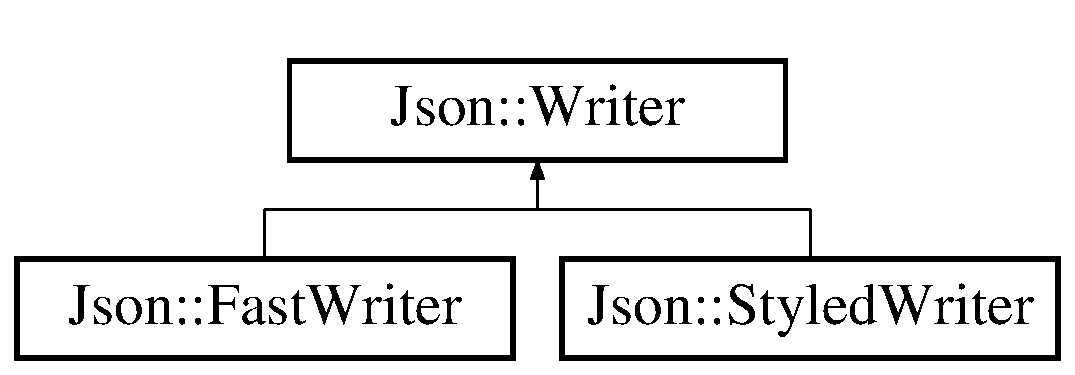
\includegraphics[height=2.000000cm]{class_json_1_1_writer}
\end{center}
\end{figure}
\subsection*{Public Member Functions}
\begin{DoxyCompactItemize}
\item 
virtual \hyperlink{class_json_1_1_writer_a3e618564336f26b14921f0d840db668c}{$\sim$\-Writer} ()
\item 
virtual std\-::string \hyperlink{class_json_1_1_writer_a7b2273a4ffd6f32b369ac8a53b7b5a0d}{write} (const \hyperlink{class_json_1_1_value}{Value} \&root)=0
\end{DoxyCompactItemize}


\subsection{Detailed Description}
Abstract class for writers. 

Definition at line 1786 of file json.\-hpp.



\subsection{Constructor \& Destructor Documentation}
\hypertarget{class_json_1_1_writer_a3e618564336f26b14921f0d840db668c}{\index{Json\-::\-Writer@{Json\-::\-Writer}!$\sim$\-Writer@{$\sim$\-Writer}}
\index{$\sim$\-Writer@{$\sim$\-Writer}!Json::Writer@{Json\-::\-Writer}}
\subsubsection[{$\sim$\-Writer}]{\setlength{\rightskip}{0pt plus 5cm}Json\-::\-Writer\-::$\sim$\-Writer (
\begin{DoxyParamCaption}
{}
\end{DoxyParamCaption}
)\hspace{0.3cm}{\ttfamily [virtual]}}}\label{class_json_1_1_writer_a3e618564336f26b14921f0d840db668c}


Definition at line 3139 of file json.\-cpp.



\subsection{Member Function Documentation}
\hypertarget{class_json_1_1_writer_a7b2273a4ffd6f32b369ac8a53b7b5a0d}{\index{Json\-::\-Writer@{Json\-::\-Writer}!write@{write}}
\index{write@{write}!Json::Writer@{Json\-::\-Writer}}
\subsubsection[{write}]{\setlength{\rightskip}{0pt plus 5cm}virtual std\-::string Json\-::\-Writer\-::write (
\begin{DoxyParamCaption}
\item[{const {\bf Value} \&}]{root}
\end{DoxyParamCaption}
)\hspace{0.3cm}{\ttfamily [pure virtual]}}}\label{class_json_1_1_writer_a7b2273a4ffd6f32b369ac8a53b7b5a0d}


Implemented in \hyperlink{class_json_1_1_styled_writer_a56f0fd80f60272b3f3c85690aae66e7d}{Json\-::\-Styled\-Writer}, and \hyperlink{class_json_1_1_fast_writer_aa66218a56447222f91d64db618935a19}{Json\-::\-Fast\-Writer}.



The documentation for this class was generated from the following files\-:\begin{DoxyCompactItemize}
\item 
includes/util/json/\hyperlink{json_8hpp}{json.\-hpp}\item 
src/util/json/\hyperlink{json_8cpp}{json.\-cpp}\end{DoxyCompactItemize}

\chapter{File Documentation}
\hypertarget{epidemics_8d}{\section{build/obj/native/\-Debug/amon/epidemics.d File Reference}
\label{epidemics_8d}\index{build/obj/native/\-Debug/amon/epidemics.\-d@{build/obj/native/\-Debug/amon/epidemics.\-d}}
}

\hypertarget{fenwick_8d}{\section{build/obj/native/\-Debug/amon/fenwick.d File Reference}
\label{fenwick_8d}\index{build/obj/native/\-Debug/amon/fenwick.\-d@{build/obj/native/\-Debug/amon/fenwick.\-d}}
}

\hypertarget{graph_8d}{\section{/home/fushigisama/\-Documents/amon/build/graph/obj/\-Debug/graph.d File Reference}
\label{graph_8d}\index{/home/fushigisama/\-Documents/amon/build/graph/obj/\-Debug/graph.\-d@{/home/fushigisama/\-Documents/amon/build/graph/obj/\-Debug/graph.\-d}}
}

\hypertarget{information__spread_8d}{\section{build/obj/native/\-Debug/amon/information\-\_\-spread.d File Reference}
\label{information__spread_8d}\index{build/obj/native/\-Debug/amon/information\-\_\-spread.\-d@{build/obj/native/\-Debug/amon/information\-\_\-spread.\-d}}
}

\hypertarget{json_8d}{\section{/home/fushigisama/\-Documents/amon/build/util/obj/\-Debug/json.d File Reference}
\label{json_8d}\index{/home/fushigisama/\-Documents/amon/build/util/obj/\-Debug/json.\-d@{/home/fushigisama/\-Documents/amon/build/util/obj/\-Debug/json.\-d}}
}

\hypertarget{network__models_8d}{\section{build/obj/native/\-Debug/amon/network\-\_\-models.d File Reference}
\label{network__models_8d}\index{build/obj/native/\-Debug/amon/network\-\_\-models.\-d@{build/obj/native/\-Debug/amon/network\-\_\-models.\-d}}
}

\hypertarget{progress__bar_8d}{\section{build/obj/native/\-Debug/amon/progress\-\_\-bar.d File Reference}
\label{progress__bar_8d}\index{build/obj/native/\-Debug/amon/progress\-\_\-bar.\-d@{build/obj/native/\-Debug/amon/progress\-\_\-bar.\-d}}
}

\hypertarget{social__networks_8d}{\section{build/obj/native/\-Debug/amon/social\-\_\-networks.d File Reference}
\label{social__networks_8d}\index{build/obj/native/\-Debug/amon/social\-\_\-networks.\-d@{build/obj/native/\-Debug/amon/social\-\_\-networks.\-d}}
}

\hypertarget{twitter_8d}{\section{build/obj/native/\-Debug/amon/twitter.d File Reference}
\label{twitter_8d}\index{build/obj/native/\-Debug/amon/twitter.\-d@{build/obj/native/\-Debug/amon/twitter.\-d}}
}

\hypertarget{amon_8d}{\section{/home/fushigisama/\-Documents/amon/build/\-Amon/obj/\-Debug/amon.d File Reference}
\label{amon_8d}\index{/home/fushigisama/\-Documents/amon/build/\-Amon/obj/\-Debug/amon.\-d@{/home/fushigisama/\-Documents/amon/build/\-Amon/obj/\-Debug/amon.\-d}}
}

\hypertarget{epidemics_8hpp}{\section{/home/fushigisama/\-Documents/amon/includes/csys/epidemics.hpp File Reference}
\label{epidemics_8hpp}\index{/home/fushigisama/\-Documents/amon/includes/csys/epidemics.\-hpp@{/home/fushigisama/\-Documents/amon/includes/csys/epidemics.\-hpp}}
}
{\ttfamily \#include $<$graph.\-hpp$>$}\\*
{\ttfamily \#include $<$vector$>$}\\*
{\ttfamily \#include $<$random$>$}\\*
\subsection*{Classes}
\begin{DoxyCompactItemize}
\item 
class \hyperlink{classamon_1_1_s_i_s_model}{amon\-::\-S\-I\-S\-Model}
\end{DoxyCompactItemize}
\subsection*{Namespaces}
\begin{DoxyCompactItemize}
\item 
\hyperlink{namespaceamon}{amon}
\end{DoxyCompactItemize}

\hypertarget{information__spread_8hpp}{\section{includes/csys/information\-\_\-spread.hpp File Reference}
\label{information__spread_8hpp}\index{includes/csys/information\-\_\-spread.\-hpp@{includes/csys/information\-\_\-spread.\-hpp}}
}
{\ttfamily \#include $<$vector$>$}\\*
{\ttfamily \#include $<$graph/graph.\-hpp$>$}\\*
{\ttfamily \#include $<$thread$>$}\\*
\subsection*{Classes}
\begin{DoxyCompactItemize}
\item 
class \hyperlink{classamon_1_1_information_network}{amon\-::\-Information\-Network}
\begin{DoxyCompactList}\small\item\em \{ Provides analysis on networks that represent information spread from people to people. \} \end{DoxyCompactList}\end{DoxyCompactItemize}
\subsection*{Namespaces}
\begin{DoxyCompactItemize}
\item 
\hyperlink{namespaceamon}{amon}
\end{DoxyCompactItemize}

\hypertarget{network__models_8hpp}{\section{includes/csys/network\-\_\-models.hpp File Reference}
\label{network__models_8hpp}\index{includes/csys/network\-\_\-models.\-hpp@{includes/csys/network\-\_\-models.\-hpp}}
}
{\ttfamily \#include $<$graph/graph.\-hpp$>$}\\*
{\ttfamily \#include $<$random$>$}\\*
\subsection*{Classes}
\begin{DoxyCompactItemize}
\item 
class \hyperlink{classamon_1_1_network_generator}{amon\-::\-Network\-Generator}
\end{DoxyCompactItemize}
\subsection*{Namespaces}
\begin{DoxyCompactItemize}
\item 
\hyperlink{namespaceamon}{amon}
\end{DoxyCompactItemize}

\hypertarget{graph_8hpp}{\section{includes/graph/graph.hpp File Reference}
\label{graph_8hpp}\index{includes/graph/graph.\-hpp@{includes/graph/graph.\-hpp}}
}
{\ttfamily \#include $<$vector$>$}\\*
{\ttfamily \#include $<$string$>$}\\*
{\ttfamily \#include $<$set$>$}\\*
{\ttfamily \#include $<$queue$>$}\\*
{\ttfamily \#include $<$utility$>$}\\*
{\ttfamily \#include $<$list$>$}\\*
{\ttfamily \#include $<$map$>$}\\*
{\ttfamily \#include $<$unordered\-\_\-map$>$}\\*
\subsection*{Classes}
\begin{DoxyCompactItemize}
\item 
class \hyperlink{classamon_1_1_graph}{amon\-::\-Graph}
\end{DoxyCompactItemize}
\subsection*{Namespaces}
\begin{DoxyCompactItemize}
\item 
\hyperlink{namespaceamon}{amon}
\end{DoxyCompactItemize}

\hypertarget{twitter_8hpp}{\section{includes/social/twitter.hpp File Reference}
\label{twitter_8hpp}\index{includes/social/twitter.\-hpp@{includes/social/twitter.\-hpp}}
}
{\ttfamily \#include $<$graph/graph.\-hpp$>$}\\*
{\ttfamily \#include $<$util/json/json.\-hpp$>$}\\*
{\ttfamily \#include $<$string$>$}\\*
{\ttfamily \#include $<$queue$>$}\\*
{\ttfamily \#include $<$fstream$>$}\\*
{\ttfamily \#include $<$unordered\-\_\-map$>$}\\*
{\ttfamily \#include $<$vector$>$}\\*
{\ttfamily \#include $<$mutex$>$}\\*
{\ttfamily \#include $<$thread$>$}\\*
\subsection*{Classes}
\begin{DoxyCompactItemize}
\item 
class \hyperlink{classamon_1_1_tweet_loader}{amon\-::\-Tweet\-Loader}
\end{DoxyCompactItemize}
\subsection*{Namespaces}
\begin{DoxyCompactItemize}
\item 
\hyperlink{namespaceamon}{amon}
\end{DoxyCompactItemize}

\hypertarget{fenwick_8hpp}{\section{/home/fushigisama/\-Documents/amon/includes/util/fenwick.hpp File Reference}
\label{fenwick_8hpp}\index{/home/fushigisama/\-Documents/amon/includes/util/fenwick.\-hpp@{/home/fushigisama/\-Documents/amon/includes/util/fenwick.\-hpp}}
}
{\ttfamily \#include $<$vector$>$}\\*
\subsection*{Classes}
\begin{DoxyCompactItemize}
\item 
class \hyperlink{classamon_1_1_fenwick_tree}{amon\-::\-Fenwick\-Tree}
\end{DoxyCompactItemize}
\subsection*{Namespaces}
\begin{DoxyCompactItemize}
\item 
\hyperlink{namespaceamon}{amon}
\end{DoxyCompactItemize}

\hypertarget{json_8hpp}{\section{includes/util/json/json.hpp File Reference}
\label{json_8hpp}\index{includes/util/json/json.\-hpp@{includes/util/json/json.\-hpp}}
}
{\ttfamily \#include $<$string$>$}\\*
{\ttfamily \#include $<$vector$>$}\\*
{\ttfamily \#include $<$map$>$}\\*
{\ttfamily \#include $<$deque$>$}\\*
{\ttfamily \#include $<$iosfwd$>$}\\*
{\ttfamily \#include $<$stack$>$}\\*
{\ttfamily \#include $<$stdlib.\-h$>$}\\*
{\ttfamily \#include $<$stdexcept$>$}\\*
\subsection*{Classes}
\begin{DoxyCompactItemize}
\item 
class \hyperlink{class_json_1_1_features}{Json\-::\-Features}
\begin{DoxyCompactList}\small\item\em Configuration passed to reader and writer. This configuration object can be used to force the \hyperlink{class_json_1_1_reader}{Reader} or \hyperlink{class_json_1_1_writer}{Writer} to behave in a standard conforming way. \end{DoxyCompactList}\item 
class \hyperlink{class_json_1_1_static_string}{Json\-::\-Static\-String}
\begin{DoxyCompactList}\small\item\em Lightweight wrapper to tag static string. \end{DoxyCompactList}\item 
class \hyperlink{class_json_1_1_value}{Json\-::\-Value}
\begin{DoxyCompactList}\small\item\em Represents a \href{http://www.json.org}{\tt J\-S\-O\-N} value. \end{DoxyCompactList}\item 
class \hyperlink{class_json_1_1_path_argument}{Json\-::\-Path\-Argument}
\begin{DoxyCompactList}\small\item\em Experimental and untested\-: represents an element of the \char`\"{}path\char`\"{} to access a node. \end{DoxyCompactList}\item 
class \hyperlink{class_json_1_1_path}{Json\-::\-Path}
\begin{DoxyCompactList}\small\item\em Experimental and untested\-: represents a \char`\"{}path\char`\"{} to access a node. \end{DoxyCompactList}\item 
class \hyperlink{class_json_1_1_value_iterator_base}{Json\-::\-Value\-Iterator\-Base}
\begin{DoxyCompactList}\small\item\em base class for \hyperlink{class_json_1_1_value}{Value} iterators. \end{DoxyCompactList}\item 
class \hyperlink{class_json_1_1_value_const_iterator}{Json\-::\-Value\-Const\-Iterator}
\begin{DoxyCompactList}\small\item\em const iterator for object and array value. \end{DoxyCompactList}\item 
class \hyperlink{class_json_1_1_value_iterator}{Json\-::\-Value\-Iterator}
\begin{DoxyCompactList}\small\item\em Iterator for object and array value. \end{DoxyCompactList}\item 
class \hyperlink{class_json_1_1_reader}{Json\-::\-Reader}
\begin{DoxyCompactList}\small\item\em Unserialize a \href{http://www.json.org}{\tt J\-S\-O\-N} document into a \hyperlink{class_json_1_1_value}{Value}. \end{DoxyCompactList}\item 
struct \hyperlink{struct_json_1_1_reader_1_1_structured_error}{Json\-::\-Reader\-::\-Structured\-Error}
\begin{DoxyCompactList}\small\item\em An error tagged with where in the J\-S\-O\-N text it was encountered. \end{DoxyCompactList}\item 
class \hyperlink{class_json_1_1_writer}{Json\-::\-Writer}
\begin{DoxyCompactList}\small\item\em Abstract class for writers. \end{DoxyCompactList}\item 
class \hyperlink{class_json_1_1_fast_writer}{Json\-::\-Fast\-Writer}
\begin{DoxyCompactList}\small\item\em Outputs a \hyperlink{class_json_1_1_value}{Value} in \href{http://www.json.org}{\tt J\-S\-O\-N} format without formatting (not human friendly). \end{DoxyCompactList}\item 
class \hyperlink{class_json_1_1_styled_writer}{Json\-::\-Styled\-Writer}
\begin{DoxyCompactList}\small\item\em Writes a \hyperlink{class_json_1_1_value}{Value} in \href{http://www.json.org}{\tt J\-S\-O\-N} format in a human friendly way. \end{DoxyCompactList}\item 
class \hyperlink{class_json_1_1_styled_stream_writer}{Json\-::\-Styled\-Stream\-Writer}
\begin{DoxyCompactList}\small\item\em Writes a \hyperlink{class_json_1_1_value}{Value} in \href{http://www.json.org}{\tt J\-S\-O\-N} format in a human friendly way, to a stream rather than to a string. \end{DoxyCompactList}\end{DoxyCompactItemize}
\subsection*{Namespaces}
\begin{DoxyCompactItemize}
\item 
\hyperlink{namespace_json}{Json}
\begin{DoxyCompactList}\small\item\em J\-S\-O\-N (Java\-Script Object Notation). \end{DoxyCompactList}\end{DoxyCompactItemize}
\subsection*{Macros}
\begin{DoxyCompactItemize}
\item 
\#define \hyperlink{json_8hpp_a1bf16856b5e907aa83ed7bc825bc5ecf}{J\-S\-O\-N\-\_\-\-I\-S\-\_\-\-A\-M\-A\-L\-G\-A\-M\-A\-T\-I\-O\-N}
\item 
\#define \hyperlink{json_8hpp_a48e81f641ee4bf786daa3fe6090aac9e}{J\-S\-O\-N\-\_\-\-V\-E\-R\-S\-I\-O\-N\-\_\-\-H\-\_\-\-I\-N\-C\-L\-U\-D\-E\-D}
\item 
\#define \hyperlink{json_8hpp_ac2869039a8826da9d06800ad2b39ed9c}{J\-S\-O\-N\-C\-P\-P\-\_\-\-V\-E\-R\-S\-I\-O\-N\-\_\-\-S\-T\-R\-I\-N\-G}~\char`\"{}1.\-0.\-0\char`\"{}
\item 
\#define \hyperlink{json_8hpp_a3a512184f0bbdd531fe1298f0a490ffe}{J\-S\-O\-N\-C\-P\-P\-\_\-\-V\-E\-R\-S\-I\-O\-N\-\_\-\-M\-A\-J\-O\-R}~1
\item 
\#define \hyperlink{json_8hpp_a8c16a078ac4151f4e9c07b04358b2550}{J\-S\-O\-N\-C\-P\-P\-\_\-\-V\-E\-R\-S\-I\-O\-N\-\_\-\-M\-I\-N\-O\-R}~0
\item 
\#define \hyperlink{json_8hpp_aaecbbae4c271193dd5bf70aa0662e66b}{J\-S\-O\-N\-C\-P\-P\-\_\-\-V\-E\-R\-S\-I\-O\-N\-\_\-\-P\-A\-T\-C\-H}~0
\item 
\#define \hyperlink{json_8hpp_a72fa63858b73149d97ad8b3d059373ce}{J\-S\-O\-N\-C\-P\-P\-\_\-\-V\-E\-R\-S\-I\-O\-N\-\_\-\-Q\-U\-A\-L\-I\-F\-I\-E\-R}
\item 
\#define \hyperlink{json_8hpp_a32ef47886b186f98d3f8225a513c3495}{J\-S\-O\-N\-C\-P\-P\-\_\-\-V\-E\-R\-S\-I\-O\-N\-\_\-\-H\-E\-X\-A}~((\hyperlink{json_8hpp_a3a512184f0bbdd531fe1298f0a490ffe}{J\-S\-O\-N\-C\-P\-P\-\_\-\-V\-E\-R\-S\-I\-O\-N\-\_\-\-M\-A\-J\-O\-R} $<$$<$ 24) $\vert$ (\hyperlink{json_8hpp_a8c16a078ac4151f4e9c07b04358b2550}{J\-S\-O\-N\-C\-P\-P\-\_\-\-V\-E\-R\-S\-I\-O\-N\-\_\-\-M\-I\-N\-O\-R} $<$$<$ 16) $\vert$ (\hyperlink{json_8hpp_aaecbbae4c271193dd5bf70aa0662e66b}{J\-S\-O\-N\-C\-P\-P\-\_\-\-V\-E\-R\-S\-I\-O\-N\-\_\-\-P\-A\-T\-C\-H} $<$$<$ 8))
\item 
\#define \hyperlink{json_8hpp_a71f1a94bee4773f2a6e30eeac7deb963}{J\-S\-O\-N\-\_\-\-C\-O\-N\-F\-I\-G\-\_\-\-H\-\_\-\-I\-N\-C\-L\-U\-D\-E\-D}
\item 
\#define \hyperlink{json_8hpp_a51968e67b1462ac893f87a0fc8b791cd}{J\-S\-O\-N\-\_\-\-U\-S\-E\-\_\-\-E\-X\-C\-E\-P\-T\-I\-O\-N}~1
\begin{DoxyCompactList}\small\item\em If defined, indicates that json library is embedded in Cpp\-T\-L library. \end{DoxyCompactList}\item 
\#define \hyperlink{json_8hpp_a1d61ffde86ce1a18fd83194ff0d9a206}{J\-S\-O\-N\-\_\-\-A\-P\-I}
\item 
\#define \hyperlink{json_8hpp_a6933a4321aa03c8a29016669073f1af6}{J\-S\-O\-N\-C\-P\-P\-\_\-\-D\-E\-P\-R\-E\-C\-A\-T\-E\-D}(message)
\item 
\#define \hyperlink{json_8hpp_a210f7d060accd6a881cd070dc7a333a4}{J\-S\-O\-N\-\_\-\-H\-A\-S\-\_\-\-I\-N\-T64}
\item 
\#define \hyperlink{json_8hpp_ac320ccec4dca293f3f50f35f7a595f3b}{J\-S\-O\-N\-\_\-\-F\-O\-R\-W\-A\-R\-D\-S\-\_\-\-H\-\_\-\-I\-N\-C\-L\-U\-D\-E\-D}
\item 
\#define \hyperlink{json_8hpp_a7f6fdcb52225adbb2c7c641919eedb5e}{C\-P\-P\-T\-L\-\_\-\-J\-S\-O\-N\-\_\-\-F\-E\-A\-T\-U\-R\-E\-S\-\_\-\-H\-\_\-\-I\-N\-C\-L\-U\-D\-E\-D}
\item 
\#define \hyperlink{json_8hpp_ace47a954331dfcdb43c7c01201b4215b}{C\-P\-P\-T\-L\-\_\-\-J\-S\-O\-N\-\_\-\-H\-\_\-\-I\-N\-C\-L\-U\-D\-E\-D}
\item 
\#define \hyperlink{json_8hpp_a474bdd38a6f0d733485d831d9d99faa2}{C\-P\-P\-T\-L\-\_\-\-J\-S\-O\-N\-\_\-\-R\-E\-A\-D\-E\-R\-\_\-\-H\-\_\-\-I\-N\-C\-L\-U\-D\-E\-D}
\item 
\#define \hyperlink{json_8hpp_a70febbb14e183c3d2beb727cd572ae36}{J\-S\-O\-N\-\_\-\-W\-R\-I\-T\-E\-R\-\_\-\-H\-\_\-\-I\-N\-C\-L\-U\-D\-E\-D}
\item 
\#define \hyperlink{json_8hpp_a79684c4b554cc59240b94eaf9a98133c}{C\-P\-P\-T\-L\-\_\-\-J\-S\-O\-N\-\_\-\-A\-S\-S\-E\-R\-T\-I\-O\-N\-S\-\_\-\-H\-\_\-\-I\-N\-C\-L\-U\-D\-E\-D}
\item 
\#define \hyperlink{json_8hpp_a188941dcc789ccb6539c3d6f41405582}{J\-S\-O\-N\-\_\-\-A\-S\-S\-E\-R\-T}(condition)~assert(condition);
\item 
\#define \hyperlink{json_8hpp_a67007439f94bc6afc465923f56147ba1}{J\-S\-O\-N\-\_\-\-F\-A\-I\-L\-\_\-\-M\-E\-S\-S\-A\-G\-E}(message)~throw std\-::runtime\-\_\-error(message);
\item 
\#define \hyperlink{json_8hpp_ad7facdeeca0f495765e3b204c265eadb}{J\-S\-O\-N\-\_\-\-A\-S\-S\-E\-R\-T\-\_\-\-M\-E\-S\-S\-A\-G\-E}(condition, message)
\end{DoxyCompactItemize}
\subsection*{Typedefs}
\begin{DoxyCompactItemize}
\item 
typedef int \hyperlink{namespace_json_a08122e8005b706d982e48cca1e2119c7}{Json\-::\-Int}
\item 
typedef unsigned int \hyperlink{namespace_json_a800fb90eb6ee8d5d62b600c06f87f7d4}{Json\-::\-U\-Int}
\item 
typedef long long int \hyperlink{namespace_json_ab7b47d2905da3b4ae60e4e800ec9ae5f}{Json\-::\-Int64}
\item 
typedef unsigned long long int \hyperlink{namespace_json_a01f20bce8f8229f38ff890168c0e6452}{Json\-::\-U\-Int64}
\item 
typedef Int64 \hyperlink{namespace_json_a218d880af853ce786cd985e82571d297}{Json\-::\-Largest\-Int}
\item 
typedef U\-Int64 \hyperlink{namespace_json_ae202ecad69725e23443f465e257456d0}{Json\-::\-Largest\-U\-Int}
\item 
typedef unsigned int \hyperlink{namespace_json_a8048e741f2177c3b5d9ede4a5b8c53c2}{Json\-::\-Array\-Index}
\end{DoxyCompactItemize}
\subsection*{Enumerations}
\begin{DoxyCompactItemize}
\item 
enum \hyperlink{namespace_json_a7d654b75c16a57007925868e38212b4e}{Json\-::\-Value\-Type} \{ \\*
\hyperlink{namespace_json_a7d654b75c16a57007925868e38212b4ea7d9899633b4409bd3fc107e6737f8391}{Json\-::null\-Value} = 0, 
\hyperlink{namespace_json_a7d654b75c16a57007925868e38212b4eae5a9d708d5c9e23ae9bf98898522512d}{Json\-::int\-Value}, 
\hyperlink{namespace_json_a7d654b75c16a57007925868e38212b4eaea788d9a3bb00adc6d68d97d43e1ccd3}{Json\-::uint\-Value}, 
\hyperlink{namespace_json_a7d654b75c16a57007925868e38212b4eab837c7b869c14d8be712deb45c9e490e}{Json\-::real\-Value}, 
\\*
\hyperlink{namespace_json_a7d654b75c16a57007925868e38212b4ea804ef857affea2d415843c73f261c258}{Json\-::string\-Value}, 
\hyperlink{namespace_json_a7d654b75c16a57007925868e38212b4ea14c30dbf4da86f7b809be299f671f7fd}{Json\-::boolean\-Value}, 
\hyperlink{namespace_json_a7d654b75c16a57007925868e38212b4eadc8f264f36b55b063c78126b335415f4}{Json\-::array\-Value}, 
\hyperlink{namespace_json_a7d654b75c16a57007925868e38212b4eae8386dcfc36d1ae897745f7b4f77a1f6}{Json\-::object\-Value}
 \}
\begin{DoxyCompactList}\small\item\em Type of the value held by a Value object. \end{DoxyCompactList}\item 
enum \hyperlink{namespace_json_a4fc417c23905b2ae9e2c47d197a45351}{Json\-::\-Comment\-Placement} \{ \hyperlink{namespace_json_a4fc417c23905b2ae9e2c47d197a45351a52f1733775460517b2ea6bedf4906d52}{Json\-::comment\-Before} = 0, 
\hyperlink{namespace_json_a4fc417c23905b2ae9e2c47d197a45351a008a230a0586de54f30b76afe70fdcfa}{Json\-::comment\-After\-On\-Same\-Line}, 
\hyperlink{namespace_json_a4fc417c23905b2ae9e2c47d197a45351ac5784ca53b12250888ddb642b06aebef}{Json\-::comment\-After}, 
\hyperlink{namespace_json_a4fc417c23905b2ae9e2c47d197a45351abcbd3eb00417335e094e4a03379659b5}{Json\-::number\-Of\-Comment\-Placement}
 \}
\end{DoxyCompactItemize}
\subsection*{Functions}
\begin{DoxyCompactItemize}
\item 
\hyperlink{json_8hpp_a1d61ffde86ce1a18fd83194ff0d9a206}{J\-S\-O\-N\-\_\-\-A\-P\-I} std\-::istream \& \hyperlink{namespace_json_a4d245ef719cc0853e8e78eb5f99c16e5}{Json\-::operator$>$$>$} (std\-::istream \&, Value \&)
\begin{DoxyCompactList}\small\item\em Read from 'sin' into 'root'. \end{DoxyCompactList}\item 
std\-::string \hyperlink{json_8hpp_a1d61ffde86ce1a18fd83194ff0d9a206}{J\-S\-O\-N\-\_\-\-A\-P\-I} \hyperlink{namespace_json_a05cd078d8e086a4bcc08d40948f711e7}{Json\-::value\-To\-String} (Int value)
\item 
std\-::string \hyperlink{json_8hpp_a1d61ffde86ce1a18fd83194ff0d9a206}{J\-S\-O\-N\-\_\-\-A\-P\-I} \hyperlink{namespace_json_abcb58ea0f384c30608729a94d539e2ce}{Json\-::value\-To\-String} (U\-Int value)
\item 
std\-::string \hyperlink{json_8hpp_a1d61ffde86ce1a18fd83194ff0d9a206}{J\-S\-O\-N\-\_\-\-A\-P\-I} \hyperlink{namespace_json_abd9c650f70d9434f98f9025e2e2faf2d}{Json\-::value\-To\-String} (Largest\-Int value)
\item 
std\-::string \hyperlink{json_8hpp_a1d61ffde86ce1a18fd83194ff0d9a206}{J\-S\-O\-N\-\_\-\-A\-P\-I} \hyperlink{namespace_json_a3f46b0bc62b95a9426a2da0117bdf9f0}{Json\-::value\-To\-String} (Largest\-U\-Int value)
\item 
std\-::string \hyperlink{json_8hpp_a1d61ffde86ce1a18fd83194ff0d9a206}{J\-S\-O\-N\-\_\-\-A\-P\-I} \hyperlink{namespace_json_a99995d7dafa4f4970b349d7d3c8d1d99}{Json\-::value\-To\-String} (double value)
\item 
std\-::string \hyperlink{json_8hpp_a1d61ffde86ce1a18fd83194ff0d9a206}{J\-S\-O\-N\-\_\-\-A\-P\-I} \hyperlink{namespace_json_a979ed531f091985e22f0051cd2a8e341}{Json\-::value\-To\-String} (bool value)
\item 
std\-::string \hyperlink{json_8hpp_a1d61ffde86ce1a18fd83194ff0d9a206}{J\-S\-O\-N\-\_\-\-A\-P\-I} \hyperlink{namespace_json_aa0c8235a4a5c6599da5d3332743db8ac}{Json\-::value\-To\-Quoted\-String} (const char $\ast$value)
\item 
\hyperlink{json_8hpp_a1d61ffde86ce1a18fd83194ff0d9a206}{J\-S\-O\-N\-\_\-\-A\-P\-I} std\-::ostream \& \hyperlink{namespace_json_a87bc83d7e90fc666d28aa16727deda2f}{Json\-::operator$<$$<$} (std\-::ostream \&, const Value \&root)
\begin{DoxyCompactList}\small\item\em Output using the \hyperlink{class_json_1_1_styled_stream_writer}{Styled\-Stream\-Writer}. \end{DoxyCompactList}\end{DoxyCompactItemize}


\subsection{Macro Definition Documentation}
\hypertarget{json_8hpp_a79684c4b554cc59240b94eaf9a98133c}{\index{json.\-hpp@{json.\-hpp}!C\-P\-P\-T\-L\-\_\-\-J\-S\-O\-N\-\_\-\-A\-S\-S\-E\-R\-T\-I\-O\-N\-S\-\_\-\-H\-\_\-\-I\-N\-C\-L\-U\-D\-E\-D@{C\-P\-P\-T\-L\-\_\-\-J\-S\-O\-N\-\_\-\-A\-S\-S\-E\-R\-T\-I\-O\-N\-S\-\_\-\-H\-\_\-\-I\-N\-C\-L\-U\-D\-E\-D}}
\index{C\-P\-P\-T\-L\-\_\-\-J\-S\-O\-N\-\_\-\-A\-S\-S\-E\-R\-T\-I\-O\-N\-S\-\_\-\-H\-\_\-\-I\-N\-C\-L\-U\-D\-E\-D@{C\-P\-P\-T\-L\-\_\-\-J\-S\-O\-N\-\_\-\-A\-S\-S\-E\-R\-T\-I\-O\-N\-S\-\_\-\-H\-\_\-\-I\-N\-C\-L\-U\-D\-E\-D}!json.hpp@{json.\-hpp}}
\subsubsection[{C\-P\-P\-T\-L\-\_\-\-J\-S\-O\-N\-\_\-\-A\-S\-S\-E\-R\-T\-I\-O\-N\-S\-\_\-\-H\-\_\-\-I\-N\-C\-L\-U\-D\-E\-D}]{\setlength{\rightskip}{0pt plus 5cm}\#define C\-P\-P\-T\-L\-\_\-\-J\-S\-O\-N\-\_\-\-A\-S\-S\-E\-R\-T\-I\-O\-N\-S\-\_\-\-H\-\_\-\-I\-N\-C\-L\-U\-D\-E\-D}}\label{json_8hpp_a79684c4b554cc59240b94eaf9a98133c}


Definition at line 1992 of file json.\-hpp.

\hypertarget{json_8hpp_a7f6fdcb52225adbb2c7c641919eedb5e}{\index{json.\-hpp@{json.\-hpp}!C\-P\-P\-T\-L\-\_\-\-J\-S\-O\-N\-\_\-\-F\-E\-A\-T\-U\-R\-E\-S\-\_\-\-H\-\_\-\-I\-N\-C\-L\-U\-D\-E\-D@{C\-P\-P\-T\-L\-\_\-\-J\-S\-O\-N\-\_\-\-F\-E\-A\-T\-U\-R\-E\-S\-\_\-\-H\-\_\-\-I\-N\-C\-L\-U\-D\-E\-D}}
\index{C\-P\-P\-T\-L\-\_\-\-J\-S\-O\-N\-\_\-\-F\-E\-A\-T\-U\-R\-E\-S\-\_\-\-H\-\_\-\-I\-N\-C\-L\-U\-D\-E\-D@{C\-P\-P\-T\-L\-\_\-\-J\-S\-O\-N\-\_\-\-F\-E\-A\-T\-U\-R\-E\-S\-\_\-\-H\-\_\-\-I\-N\-C\-L\-U\-D\-E\-D}!json.hpp@{json.\-hpp}}
\subsubsection[{C\-P\-P\-T\-L\-\_\-\-J\-S\-O\-N\-\_\-\-F\-E\-A\-T\-U\-R\-E\-S\-\_\-\-H\-\_\-\-I\-N\-C\-L\-U\-D\-E\-D}]{\setlength{\rightskip}{0pt plus 5cm}\#define C\-P\-P\-T\-L\-\_\-\-J\-S\-O\-N\-\_\-\-F\-E\-A\-T\-U\-R\-E\-S\-\_\-\-H\-\_\-\-I\-N\-C\-L\-U\-D\-E\-D}}\label{json_8hpp_a7f6fdcb52225adbb2c7c641919eedb5e}


Definition at line 302 of file json.\-hpp.

\hypertarget{json_8hpp_ace47a954331dfcdb43c7c01201b4215b}{\index{json.\-hpp@{json.\-hpp}!C\-P\-P\-T\-L\-\_\-\-J\-S\-O\-N\-\_\-\-H\-\_\-\-I\-N\-C\-L\-U\-D\-E\-D@{C\-P\-P\-T\-L\-\_\-\-J\-S\-O\-N\-\_\-\-H\-\_\-\-I\-N\-C\-L\-U\-D\-E\-D}}
\index{C\-P\-P\-T\-L\-\_\-\-J\-S\-O\-N\-\_\-\-H\-\_\-\-I\-N\-C\-L\-U\-D\-E\-D@{C\-P\-P\-T\-L\-\_\-\-J\-S\-O\-N\-\_\-\-H\-\_\-\-I\-N\-C\-L\-U\-D\-E\-D}!json.hpp@{json.\-hpp}}
\subsubsection[{C\-P\-P\-T\-L\-\_\-\-J\-S\-O\-N\-\_\-\-H\-\_\-\-I\-N\-C\-L\-U\-D\-E\-D}]{\setlength{\rightskip}{0pt plus 5cm}\#define C\-P\-P\-T\-L\-\_\-\-J\-S\-O\-N\-\_\-\-H\-\_\-\-I\-N\-C\-L\-U\-D\-E\-D}}\label{json_8hpp_ace47a954331dfcdb43c7c01201b4215b}


Definition at line 373 of file json.\-hpp.

\hypertarget{json_8hpp_a474bdd38a6f0d733485d831d9d99faa2}{\index{json.\-hpp@{json.\-hpp}!C\-P\-P\-T\-L\-\_\-\-J\-S\-O\-N\-\_\-\-R\-E\-A\-D\-E\-R\-\_\-\-H\-\_\-\-I\-N\-C\-L\-U\-D\-E\-D@{C\-P\-P\-T\-L\-\_\-\-J\-S\-O\-N\-\_\-\-R\-E\-A\-D\-E\-R\-\_\-\-H\-\_\-\-I\-N\-C\-L\-U\-D\-E\-D}}
\index{C\-P\-P\-T\-L\-\_\-\-J\-S\-O\-N\-\_\-\-R\-E\-A\-D\-E\-R\-\_\-\-H\-\_\-\-I\-N\-C\-L\-U\-D\-E\-D@{C\-P\-P\-T\-L\-\_\-\-J\-S\-O\-N\-\_\-\-R\-E\-A\-D\-E\-R\-\_\-\-H\-\_\-\-I\-N\-C\-L\-U\-D\-E\-D}!json.hpp@{json.\-hpp}}
\subsubsection[{C\-P\-P\-T\-L\-\_\-\-J\-S\-O\-N\-\_\-\-R\-E\-A\-D\-E\-R\-\_\-\-H\-\_\-\-I\-N\-C\-L\-U\-D\-E\-D}]{\setlength{\rightskip}{0pt plus 5cm}\#define C\-P\-P\-T\-L\-\_\-\-J\-S\-O\-N\-\_\-\-R\-E\-A\-D\-E\-R\-\_\-\-H\-\_\-\-I\-N\-C\-L\-U\-D\-E\-D}}\label{json_8hpp_a474bdd38a6f0d733485d831d9d99faa2}


Definition at line 1475 of file json.\-hpp.

\hypertarget{json_8hpp_a1d61ffde86ce1a18fd83194ff0d9a206}{\index{json.\-hpp@{json.\-hpp}!J\-S\-O\-N\-\_\-\-A\-P\-I@{J\-S\-O\-N\-\_\-\-A\-P\-I}}
\index{J\-S\-O\-N\-\_\-\-A\-P\-I@{J\-S\-O\-N\-\_\-\-A\-P\-I}!json.hpp@{json.\-hpp}}
\subsubsection[{J\-S\-O\-N\-\_\-\-A\-P\-I}]{\setlength{\rightskip}{0pt plus 5cm}\#define J\-S\-O\-N\-\_\-\-A\-P\-I}}\label{json_8hpp_a1d61ffde86ce1a18fd83194ff0d9a206}
If defined, indicates that the source file is amalgated to prevent private header inclusion. Remarks\-: it is automatically defined in the generated amalgated header. 

Definition at line 174 of file json.\-hpp.

\hypertarget{json_8hpp_a188941dcc789ccb6539c3d6f41405582}{\index{json.\-hpp@{json.\-hpp}!J\-S\-O\-N\-\_\-\-A\-S\-S\-E\-R\-T@{J\-S\-O\-N\-\_\-\-A\-S\-S\-E\-R\-T}}
\index{J\-S\-O\-N\-\_\-\-A\-S\-S\-E\-R\-T@{J\-S\-O\-N\-\_\-\-A\-S\-S\-E\-R\-T}!json.hpp@{json.\-hpp}}
\subsubsection[{J\-S\-O\-N\-\_\-\-A\-S\-S\-E\-R\-T}]{\setlength{\rightskip}{0pt plus 5cm}\#define J\-S\-O\-N\-\_\-\-A\-S\-S\-E\-R\-T(
\begin{DoxyParamCaption}
\item[{}]{condition}
\end{DoxyParamCaption}
)~assert(condition);}}\label{json_8hpp_a188941dcc789ccb6539c3d6f41405582}


Definition at line 2002 of file json.\-hpp.

\hypertarget{json_8hpp_ad7facdeeca0f495765e3b204c265eadb}{\index{json.\-hpp@{json.\-hpp}!J\-S\-O\-N\-\_\-\-A\-S\-S\-E\-R\-T\-\_\-\-M\-E\-S\-S\-A\-G\-E@{J\-S\-O\-N\-\_\-\-A\-S\-S\-E\-R\-T\-\_\-\-M\-E\-S\-S\-A\-G\-E}}
\index{J\-S\-O\-N\-\_\-\-A\-S\-S\-E\-R\-T\-\_\-\-M\-E\-S\-S\-A\-G\-E@{J\-S\-O\-N\-\_\-\-A\-S\-S\-E\-R\-T\-\_\-\-M\-E\-S\-S\-A\-G\-E}!json.hpp@{json.\-hpp}}
\subsubsection[{J\-S\-O\-N\-\_\-\-A\-S\-S\-E\-R\-T\-\_\-\-M\-E\-S\-S\-A\-G\-E}]{\setlength{\rightskip}{0pt plus 5cm}\#define J\-S\-O\-N\-\_\-\-A\-S\-S\-E\-R\-T\-\_\-\-M\-E\-S\-S\-A\-G\-E(
\begin{DoxyParamCaption}
\item[{}]{condition, }
\item[{}]{message}
\end{DoxyParamCaption}
)}}\label{json_8hpp_ad7facdeeca0f495765e3b204c265eadb}
{\bfseries Value\-:}
\begin{DoxyCode}
\textcolor{keywordflow}{if} (!(condition)) \{                                                          \hyperlink{json_8hpp_a67007439f94bc6afc465923f56147ba1}{\(\backslash\)}
\hyperlink{json_8hpp_a67007439f94bc6afc465923f56147ba1}{    JSON\_FAIL\_MESSAGE}(message)                                                 \(\backslash\)
  \}
\end{DoxyCode}


Definition at line 2021 of file json.\-hpp.

\hypertarget{json_8hpp_a71f1a94bee4773f2a6e30eeac7deb963}{\index{json.\-hpp@{json.\-hpp}!J\-S\-O\-N\-\_\-\-C\-O\-N\-F\-I\-G\-\_\-\-H\-\_\-\-I\-N\-C\-L\-U\-D\-E\-D@{J\-S\-O\-N\-\_\-\-C\-O\-N\-F\-I\-G\-\_\-\-H\-\_\-\-I\-N\-C\-L\-U\-D\-E\-D}}
\index{J\-S\-O\-N\-\_\-\-C\-O\-N\-F\-I\-G\-\_\-\-H\-\_\-\-I\-N\-C\-L\-U\-D\-E\-D@{J\-S\-O\-N\-\_\-\-C\-O\-N\-F\-I\-G\-\_\-\-H\-\_\-\-I\-N\-C\-L\-U\-D\-E\-D}!json.hpp@{json.\-hpp}}
\subsubsection[{J\-S\-O\-N\-\_\-\-C\-O\-N\-F\-I\-G\-\_\-\-H\-\_\-\-I\-N\-C\-L\-U\-D\-E\-D}]{\setlength{\rightskip}{0pt plus 5cm}\#define J\-S\-O\-N\-\_\-\-C\-O\-N\-F\-I\-G\-\_\-\-H\-\_\-\-I\-N\-C\-L\-U\-D\-E\-D}}\label{json_8hpp_a71f1a94bee4773f2a6e30eeac7deb963}


Definition at line 119 of file json.\-hpp.

\hypertarget{json_8hpp_a67007439f94bc6afc465923f56147ba1}{\index{json.\-hpp@{json.\-hpp}!J\-S\-O\-N\-\_\-\-F\-A\-I\-L\-\_\-\-M\-E\-S\-S\-A\-G\-E@{J\-S\-O\-N\-\_\-\-F\-A\-I\-L\-\_\-\-M\-E\-S\-S\-A\-G\-E}}
\index{J\-S\-O\-N\-\_\-\-F\-A\-I\-L\-\_\-\-M\-E\-S\-S\-A\-G\-E@{J\-S\-O\-N\-\_\-\-F\-A\-I\-L\-\_\-\-M\-E\-S\-S\-A\-G\-E}!json.hpp@{json.\-hpp}}
\subsubsection[{J\-S\-O\-N\-\_\-\-F\-A\-I\-L\-\_\-\-M\-E\-S\-S\-A\-G\-E}]{\setlength{\rightskip}{0pt plus 5cm}\#define J\-S\-O\-N\-\_\-\-F\-A\-I\-L\-\_\-\-M\-E\-S\-S\-A\-G\-E(
\begin{DoxyParamCaption}
\item[{}]{message}
\end{DoxyParamCaption}
)~throw std\-::runtime\-\_\-error(message);}}\label{json_8hpp_a67007439f94bc6afc465923f56147ba1}


Definition at line 2004 of file json.\-hpp.

\hypertarget{json_8hpp_ac320ccec4dca293f3f50f35f7a595f3b}{\index{json.\-hpp@{json.\-hpp}!J\-S\-O\-N\-\_\-\-F\-O\-R\-W\-A\-R\-D\-S\-\_\-\-H\-\_\-\-I\-N\-C\-L\-U\-D\-E\-D@{J\-S\-O\-N\-\_\-\-F\-O\-R\-W\-A\-R\-D\-S\-\_\-\-H\-\_\-\-I\-N\-C\-L\-U\-D\-E\-D}}
\index{J\-S\-O\-N\-\_\-\-F\-O\-R\-W\-A\-R\-D\-S\-\_\-\-H\-\_\-\-I\-N\-C\-L\-U\-D\-E\-D@{J\-S\-O\-N\-\_\-\-F\-O\-R\-W\-A\-R\-D\-S\-\_\-\-H\-\_\-\-I\-N\-C\-L\-U\-D\-E\-D}!json.hpp@{json.\-hpp}}
\subsubsection[{J\-S\-O\-N\-\_\-\-F\-O\-R\-W\-A\-R\-D\-S\-\_\-\-H\-\_\-\-I\-N\-C\-L\-U\-D\-E\-D}]{\setlength{\rightskip}{0pt plus 5cm}\#define J\-S\-O\-N\-\_\-\-F\-O\-R\-W\-A\-R\-D\-S\-\_\-\-H\-\_\-\-I\-N\-C\-L\-U\-D\-E\-D}}\label{json_8hpp_ac320ccec4dca293f3f50f35f7a595f3b}


Definition at line 245 of file json.\-hpp.

\hypertarget{json_8hpp_a210f7d060accd6a881cd070dc7a333a4}{\index{json.\-hpp@{json.\-hpp}!J\-S\-O\-N\-\_\-\-H\-A\-S\-\_\-\-I\-N\-T64@{J\-S\-O\-N\-\_\-\-H\-A\-S\-\_\-\-I\-N\-T64}}
\index{J\-S\-O\-N\-\_\-\-H\-A\-S\-\_\-\-I\-N\-T64@{J\-S\-O\-N\-\_\-\-H\-A\-S\-\_\-\-I\-N\-T64}!json.hpp@{json.\-hpp}}
\subsubsection[{J\-S\-O\-N\-\_\-\-H\-A\-S\-\_\-\-I\-N\-T64}]{\setlength{\rightskip}{0pt plus 5cm}\#define J\-S\-O\-N\-\_\-\-H\-A\-S\-\_\-\-I\-N\-T64}}\label{json_8hpp_a210f7d060accd6a881cd070dc7a333a4}


Definition at line 220 of file json.\-hpp.

\hypertarget{json_8hpp_a1bf16856b5e907aa83ed7bc825bc5ecf}{\index{json.\-hpp@{json.\-hpp}!J\-S\-O\-N\-\_\-\-I\-S\-\_\-\-A\-M\-A\-L\-G\-A\-M\-A\-T\-I\-O\-N@{J\-S\-O\-N\-\_\-\-I\-S\-\_\-\-A\-M\-A\-L\-G\-A\-M\-A\-T\-I\-O\-N}}
\index{J\-S\-O\-N\-\_\-\-I\-S\-\_\-\-A\-M\-A\-L\-G\-A\-M\-A\-T\-I\-O\-N@{J\-S\-O\-N\-\_\-\-I\-S\-\_\-\-A\-M\-A\-L\-G\-A\-M\-A\-T\-I\-O\-N}!json.hpp@{json.\-hpp}}
\subsubsection[{J\-S\-O\-N\-\_\-\-I\-S\-\_\-\-A\-M\-A\-L\-G\-A\-M\-A\-T\-I\-O\-N}]{\setlength{\rightskip}{0pt plus 5cm}\#define J\-S\-O\-N\-\_\-\-I\-S\-\_\-\-A\-M\-A\-L\-G\-A\-M\-A\-T\-I\-O\-N}}\label{json_8hpp_a1bf16856b5e907aa83ed7bc825bc5ecf}
Json-\/cpp amalgated header (\href{http://jsoncpp.sourceforge.net/}{\tt http\-://jsoncpp.\-sourceforge.\-net/}). It is intented to be used with \#include $<$json/json.\-h$>$ If defined, indicates that the source file is amalgated to prevent private header inclusion. 

Definition at line 79 of file json.\-hpp.

\hypertarget{json_8hpp_a51968e67b1462ac893f87a0fc8b791cd}{\index{json.\-hpp@{json.\-hpp}!J\-S\-O\-N\-\_\-\-U\-S\-E\-\_\-\-E\-X\-C\-E\-P\-T\-I\-O\-N@{J\-S\-O\-N\-\_\-\-U\-S\-E\-\_\-\-E\-X\-C\-E\-P\-T\-I\-O\-N}}
\index{J\-S\-O\-N\-\_\-\-U\-S\-E\-\_\-\-E\-X\-C\-E\-P\-T\-I\-O\-N@{J\-S\-O\-N\-\_\-\-U\-S\-E\-\_\-\-E\-X\-C\-E\-P\-T\-I\-O\-N}!json.hpp@{json.\-hpp}}
\subsubsection[{J\-S\-O\-N\-\_\-\-U\-S\-E\-\_\-\-E\-X\-C\-E\-P\-T\-I\-O\-N}]{\setlength{\rightskip}{0pt plus 5cm}\#define J\-S\-O\-N\-\_\-\-U\-S\-E\-\_\-\-E\-X\-C\-E\-P\-T\-I\-O\-N~1}}\label{json_8hpp_a51968e67b1462ac893f87a0fc8b791cd}


If defined, indicates that json library is embedded in Cpp\-T\-L library. 

If defined, indicates that json may leverage Cpp\-T\-L library If defined, indicates that cpptl vector based map should be used instead of std\-::map as Value container. If defined, indicates that \hyperlink{namespace_json}{Json} specific container should be used (hash table \& simple deque container with customizable allocator). T\-H\-I\-S F\-E\-A\-T\-U\-R\-E I\-S S\-T\-I\-L\-L E\-X\-P\-E\-R\-I\-M\-E\-N\-T\-A\-L! There is know bugs\-: See \#3177332 Force usage of standard new/malloc based allocator instead of memory pool based allocator. The memory pools allocator used optimization (initializing Value and Value\-Internal\-Link as if it was a P\-O\-D) that may cause some validation tool to report errors. Only has effects if J\-S\-O\-N\-\_\-\-V\-A\-L\-U\-E\-\_\-\-U\-S\-E\-\_\-\-I\-N\-T\-E\-R\-N\-A\-L\-\_\-\-M\-A\-P is defined. 

Definition at line 145 of file json.\-hpp.

\hypertarget{json_8hpp_a48e81f641ee4bf786daa3fe6090aac9e}{\index{json.\-hpp@{json.\-hpp}!J\-S\-O\-N\-\_\-\-V\-E\-R\-S\-I\-O\-N\-\_\-\-H\-\_\-\-I\-N\-C\-L\-U\-D\-E\-D@{J\-S\-O\-N\-\_\-\-V\-E\-R\-S\-I\-O\-N\-\_\-\-H\-\_\-\-I\-N\-C\-L\-U\-D\-E\-D}}
\index{J\-S\-O\-N\-\_\-\-V\-E\-R\-S\-I\-O\-N\-\_\-\-H\-\_\-\-I\-N\-C\-L\-U\-D\-E\-D@{J\-S\-O\-N\-\_\-\-V\-E\-R\-S\-I\-O\-N\-\_\-\-H\-\_\-\-I\-N\-C\-L\-U\-D\-E\-D}!json.hpp@{json.\-hpp}}
\subsubsection[{J\-S\-O\-N\-\_\-\-V\-E\-R\-S\-I\-O\-N\-\_\-\-H\-\_\-\-I\-N\-C\-L\-U\-D\-E\-D}]{\setlength{\rightskip}{0pt plus 5cm}\#define J\-S\-O\-N\-\_\-\-V\-E\-R\-S\-I\-O\-N\-\_\-\-H\-\_\-\-I\-N\-C\-L\-U\-D\-E\-D}}\label{json_8hpp_a48e81f641ee4bf786daa3fe6090aac9e}


Definition at line 89 of file json.\-hpp.

\hypertarget{json_8hpp_a70febbb14e183c3d2beb727cd572ae36}{\index{json.\-hpp@{json.\-hpp}!J\-S\-O\-N\-\_\-\-W\-R\-I\-T\-E\-R\-\_\-\-H\-\_\-\-I\-N\-C\-L\-U\-D\-E\-D@{J\-S\-O\-N\-\_\-\-W\-R\-I\-T\-E\-R\-\_\-\-H\-\_\-\-I\-N\-C\-L\-U\-D\-E\-D}}
\index{J\-S\-O\-N\-\_\-\-W\-R\-I\-T\-E\-R\-\_\-\-H\-\_\-\-I\-N\-C\-L\-U\-D\-E\-D@{J\-S\-O\-N\-\_\-\-W\-R\-I\-T\-E\-R\-\_\-\-H\-\_\-\-I\-N\-C\-L\-U\-D\-E\-D}!json.hpp@{json.\-hpp}}
\subsubsection[{J\-S\-O\-N\-\_\-\-W\-R\-I\-T\-E\-R\-\_\-\-H\-\_\-\-I\-N\-C\-L\-U\-D\-E\-D}]{\setlength{\rightskip}{0pt plus 5cm}\#define J\-S\-O\-N\-\_\-\-W\-R\-I\-T\-E\-R\-\_\-\-H\-\_\-\-I\-N\-C\-L\-U\-D\-E\-D}}\label{json_8hpp_a70febbb14e183c3d2beb727cd572ae36}


Definition at line 1765 of file json.\-hpp.

\hypertarget{json_8hpp_a6933a4321aa03c8a29016669073f1af6}{\index{json.\-hpp@{json.\-hpp}!J\-S\-O\-N\-C\-P\-P\-\_\-\-D\-E\-P\-R\-E\-C\-A\-T\-E\-D@{J\-S\-O\-N\-C\-P\-P\-\_\-\-D\-E\-P\-R\-E\-C\-A\-T\-E\-D}}
\index{J\-S\-O\-N\-C\-P\-P\-\_\-\-D\-E\-P\-R\-E\-C\-A\-T\-E\-D@{J\-S\-O\-N\-C\-P\-P\-\_\-\-D\-E\-P\-R\-E\-C\-A\-T\-E\-D}!json.hpp@{json.\-hpp}}
\subsubsection[{J\-S\-O\-N\-C\-P\-P\-\_\-\-D\-E\-P\-R\-E\-C\-A\-T\-E\-D}]{\setlength{\rightskip}{0pt plus 5cm}\#define J\-S\-O\-N\-C\-P\-P\-\_\-\-D\-E\-P\-R\-E\-C\-A\-T\-E\-D(
\begin{DoxyParamCaption}
\item[{}]{message}
\end{DoxyParamCaption}
)}}\label{json_8hpp_a6933a4321aa03c8a29016669073f1af6}


Definition at line 199 of file json.\-hpp.

\hypertarget{json_8hpp_a32ef47886b186f98d3f8225a513c3495}{\index{json.\-hpp@{json.\-hpp}!J\-S\-O\-N\-C\-P\-P\-\_\-\-V\-E\-R\-S\-I\-O\-N\-\_\-\-H\-E\-X\-A@{J\-S\-O\-N\-C\-P\-P\-\_\-\-V\-E\-R\-S\-I\-O\-N\-\_\-\-H\-E\-X\-A}}
\index{J\-S\-O\-N\-C\-P\-P\-\_\-\-V\-E\-R\-S\-I\-O\-N\-\_\-\-H\-E\-X\-A@{J\-S\-O\-N\-C\-P\-P\-\_\-\-V\-E\-R\-S\-I\-O\-N\-\_\-\-H\-E\-X\-A}!json.hpp@{json.\-hpp}}
\subsubsection[{J\-S\-O\-N\-C\-P\-P\-\_\-\-V\-E\-R\-S\-I\-O\-N\-\_\-\-H\-E\-X\-A}]{\setlength{\rightskip}{0pt plus 5cm}\#define J\-S\-O\-N\-C\-P\-P\-\_\-\-V\-E\-R\-S\-I\-O\-N\-\_\-\-H\-E\-X\-A~(({\bf J\-S\-O\-N\-C\-P\-P\-\_\-\-V\-E\-R\-S\-I\-O\-N\-\_\-\-M\-A\-J\-O\-R} $<$$<$ 24) $\vert$ ({\bf J\-S\-O\-N\-C\-P\-P\-\_\-\-V\-E\-R\-S\-I\-O\-N\-\_\-\-M\-I\-N\-O\-R} $<$$<$ 16) $\vert$ ({\bf J\-S\-O\-N\-C\-P\-P\-\_\-\-V\-E\-R\-S\-I\-O\-N\-\_\-\-P\-A\-T\-C\-H} $<$$<$ 8))}}\label{json_8hpp_a32ef47886b186f98d3f8225a513c3495}


Definition at line 96 of file json.\-hpp.

\hypertarget{json_8hpp_a3a512184f0bbdd531fe1298f0a490ffe}{\index{json.\-hpp@{json.\-hpp}!J\-S\-O\-N\-C\-P\-P\-\_\-\-V\-E\-R\-S\-I\-O\-N\-\_\-\-M\-A\-J\-O\-R@{J\-S\-O\-N\-C\-P\-P\-\_\-\-V\-E\-R\-S\-I\-O\-N\-\_\-\-M\-A\-J\-O\-R}}
\index{J\-S\-O\-N\-C\-P\-P\-\_\-\-V\-E\-R\-S\-I\-O\-N\-\_\-\-M\-A\-J\-O\-R@{J\-S\-O\-N\-C\-P\-P\-\_\-\-V\-E\-R\-S\-I\-O\-N\-\_\-\-M\-A\-J\-O\-R}!json.hpp@{json.\-hpp}}
\subsubsection[{J\-S\-O\-N\-C\-P\-P\-\_\-\-V\-E\-R\-S\-I\-O\-N\-\_\-\-M\-A\-J\-O\-R}]{\setlength{\rightskip}{0pt plus 5cm}\#define J\-S\-O\-N\-C\-P\-P\-\_\-\-V\-E\-R\-S\-I\-O\-N\-\_\-\-M\-A\-J\-O\-R~1}}\label{json_8hpp_a3a512184f0bbdd531fe1298f0a490ffe}


Definition at line 92 of file json.\-hpp.

\hypertarget{json_8hpp_a8c16a078ac4151f4e9c07b04358b2550}{\index{json.\-hpp@{json.\-hpp}!J\-S\-O\-N\-C\-P\-P\-\_\-\-V\-E\-R\-S\-I\-O\-N\-\_\-\-M\-I\-N\-O\-R@{J\-S\-O\-N\-C\-P\-P\-\_\-\-V\-E\-R\-S\-I\-O\-N\-\_\-\-M\-I\-N\-O\-R}}
\index{J\-S\-O\-N\-C\-P\-P\-\_\-\-V\-E\-R\-S\-I\-O\-N\-\_\-\-M\-I\-N\-O\-R@{J\-S\-O\-N\-C\-P\-P\-\_\-\-V\-E\-R\-S\-I\-O\-N\-\_\-\-M\-I\-N\-O\-R}!json.hpp@{json.\-hpp}}
\subsubsection[{J\-S\-O\-N\-C\-P\-P\-\_\-\-V\-E\-R\-S\-I\-O\-N\-\_\-\-M\-I\-N\-O\-R}]{\setlength{\rightskip}{0pt plus 5cm}\#define J\-S\-O\-N\-C\-P\-P\-\_\-\-V\-E\-R\-S\-I\-O\-N\-\_\-\-M\-I\-N\-O\-R~0}}\label{json_8hpp_a8c16a078ac4151f4e9c07b04358b2550}


Definition at line 93 of file json.\-hpp.

\hypertarget{json_8hpp_aaecbbae4c271193dd5bf70aa0662e66b}{\index{json.\-hpp@{json.\-hpp}!J\-S\-O\-N\-C\-P\-P\-\_\-\-V\-E\-R\-S\-I\-O\-N\-\_\-\-P\-A\-T\-C\-H@{J\-S\-O\-N\-C\-P\-P\-\_\-\-V\-E\-R\-S\-I\-O\-N\-\_\-\-P\-A\-T\-C\-H}}
\index{J\-S\-O\-N\-C\-P\-P\-\_\-\-V\-E\-R\-S\-I\-O\-N\-\_\-\-P\-A\-T\-C\-H@{J\-S\-O\-N\-C\-P\-P\-\_\-\-V\-E\-R\-S\-I\-O\-N\-\_\-\-P\-A\-T\-C\-H}!json.hpp@{json.\-hpp}}
\subsubsection[{J\-S\-O\-N\-C\-P\-P\-\_\-\-V\-E\-R\-S\-I\-O\-N\-\_\-\-P\-A\-T\-C\-H}]{\setlength{\rightskip}{0pt plus 5cm}\#define J\-S\-O\-N\-C\-P\-P\-\_\-\-V\-E\-R\-S\-I\-O\-N\-\_\-\-P\-A\-T\-C\-H~0}}\label{json_8hpp_aaecbbae4c271193dd5bf70aa0662e66b}


Definition at line 94 of file json.\-hpp.

\hypertarget{json_8hpp_a72fa63858b73149d97ad8b3d059373ce}{\index{json.\-hpp@{json.\-hpp}!J\-S\-O\-N\-C\-P\-P\-\_\-\-V\-E\-R\-S\-I\-O\-N\-\_\-\-Q\-U\-A\-L\-I\-F\-I\-E\-R@{J\-S\-O\-N\-C\-P\-P\-\_\-\-V\-E\-R\-S\-I\-O\-N\-\_\-\-Q\-U\-A\-L\-I\-F\-I\-E\-R}}
\index{J\-S\-O\-N\-C\-P\-P\-\_\-\-V\-E\-R\-S\-I\-O\-N\-\_\-\-Q\-U\-A\-L\-I\-F\-I\-E\-R@{J\-S\-O\-N\-C\-P\-P\-\_\-\-V\-E\-R\-S\-I\-O\-N\-\_\-\-Q\-U\-A\-L\-I\-F\-I\-E\-R}!json.hpp@{json.\-hpp}}
\subsubsection[{J\-S\-O\-N\-C\-P\-P\-\_\-\-V\-E\-R\-S\-I\-O\-N\-\_\-\-Q\-U\-A\-L\-I\-F\-I\-E\-R}]{\setlength{\rightskip}{0pt plus 5cm}\#define J\-S\-O\-N\-C\-P\-P\-\_\-\-V\-E\-R\-S\-I\-O\-N\-\_\-\-Q\-U\-A\-L\-I\-F\-I\-E\-R}}\label{json_8hpp_a72fa63858b73149d97ad8b3d059373ce}


Definition at line 95 of file json.\-hpp.

\hypertarget{json_8hpp_ac2869039a8826da9d06800ad2b39ed9c}{\index{json.\-hpp@{json.\-hpp}!J\-S\-O\-N\-C\-P\-P\-\_\-\-V\-E\-R\-S\-I\-O\-N\-\_\-\-S\-T\-R\-I\-N\-G@{J\-S\-O\-N\-C\-P\-P\-\_\-\-V\-E\-R\-S\-I\-O\-N\-\_\-\-S\-T\-R\-I\-N\-G}}
\index{J\-S\-O\-N\-C\-P\-P\-\_\-\-V\-E\-R\-S\-I\-O\-N\-\_\-\-S\-T\-R\-I\-N\-G@{J\-S\-O\-N\-C\-P\-P\-\_\-\-V\-E\-R\-S\-I\-O\-N\-\_\-\-S\-T\-R\-I\-N\-G}!json.hpp@{json.\-hpp}}
\subsubsection[{J\-S\-O\-N\-C\-P\-P\-\_\-\-V\-E\-R\-S\-I\-O\-N\-\_\-\-S\-T\-R\-I\-N\-G}]{\setlength{\rightskip}{0pt plus 5cm}\#define J\-S\-O\-N\-C\-P\-P\-\_\-\-V\-E\-R\-S\-I\-O\-N\-\_\-\-S\-T\-R\-I\-N\-G~\char`\"{}1.\-0.\-0\char`\"{}}}\label{json_8hpp_ac2869039a8826da9d06800ad2b39ed9c}


Definition at line 91 of file json.\-hpp.


\hypertarget{progress__bar_8hpp}{\section{includes/util/progress\-\_\-bar.hpp File Reference}
\label{progress__bar_8hpp}\index{includes/util/progress\-\_\-bar.\-hpp@{includes/util/progress\-\_\-bar.\-hpp}}
}
{\ttfamily \#include $<$ostream$>$}\\*
\subsection*{Classes}
\begin{DoxyCompactItemize}
\item 
class \hyperlink{classamon_1_1_progress_bar}{amon\-::\-Progress\-Bar}
\end{DoxyCompactItemize}
\subsection*{Namespaces}
\begin{DoxyCompactItemize}
\item 
\hyperlink{namespaceamon}{amon}
\end{DoxyCompactItemize}

\hypertarget{_r_e_a_d_m_e_8md}{\section{R\-E\-A\-D\-M\-E.\-md File Reference}
\label{_r_e_a_d_m_e_8md}\index{R\-E\-A\-D\-M\-E.\-md@{R\-E\-A\-D\-M\-E.\-md}}
}

\hypertarget{amon_8cpp}{\section{src/amon/amon.cpp File Reference}
\label{amon_8cpp}\index{src/amon/amon.\-cpp@{src/amon/amon.\-cpp}}
}
{\ttfamily \#include $<$graph/graph.\-hpp$>$}\\*
{\ttfamily \#include $<$util/json/json.\-hpp$>$}\\*
{\ttfamily \#include $<$cstdio$>$}\\*
{\ttfamily \#include $<$iostream$>$}\\*
{\ttfamily \#include $<$csys/network\-\_\-models.\-hpp$>$}\\*
{\ttfamily \#include $<$csys/epidemics.\-hpp$>$}\\*
{\ttfamily \#include $<$social/twitter.\-hpp$>$}\\*
{\ttfamily \#include $<$csys/information\-\_\-spread.\-hpp$>$}\\*
{\ttfamily \#include $<$unordered\-\_\-map$>$}\\*
\subsection*{Functions}
\begin{DoxyCompactItemize}
\item 
int \hyperlink{amon_8cpp_ac4c0f8a8146b128f1b8f920e3a9c3b1e}{main} (int argv, char $\ast$argc\mbox{[}$\,$\mbox{]})
\end{DoxyCompactItemize}


\subsection{Function Documentation}
\hypertarget{amon_8cpp_ac4c0f8a8146b128f1b8f920e3a9c3b1e}{\index{amon.\-cpp@{amon.\-cpp}!main@{main}}
\index{main@{main}!amon.cpp@{amon.\-cpp}}
\subsubsection[{main}]{\setlength{\rightskip}{0pt plus 5cm}int main (
\begin{DoxyParamCaption}
\item[{int}]{argv, }
\item[{char $\ast$}]{argc\mbox{[}$\,$\mbox{]}}
\end{DoxyParamCaption}
)}}\label{amon_8cpp_ac4c0f8a8146b128f1b8f920e3a9c3b1e}


Definition at line 15 of file amon.\-cpp.


\hypertarget{epidemics_8cpp}{\section{src/csys/epidemics.cpp File Reference}
\label{epidemics_8cpp}\index{src/csys/epidemics.\-cpp@{src/csys/epidemics.\-cpp}}
}
{\ttfamily \#include $<$csys/epidemics.\-hpp$>$}\\*
{\ttfamily \#include $<$graph/graph.\-hpp$>$}\\*
{\ttfamily \#include $<$iostream$>$}\\*

\hypertarget{information__spread_8cpp}{\section{src/csys/information\-\_\-spread.cpp File Reference}
\label{information__spread_8cpp}\index{src/csys/information\-\_\-spread.\-cpp@{src/csys/information\-\_\-spread.\-cpp}}
}
{\ttfamily \#include $<$csys/information\-\_\-spread.\-hpp$>$}\\*
{\ttfamily \#include $<$future$>$}\\*
{\ttfamily \#include $<$thread$>$}\\*
{\ttfamily \#include $<$algorithm$>$}\\*
{\ttfamily \#include $<$util/progress\-\_\-bar.\-hpp$>$}\\*
{\ttfamily \#include $<$iostream$>$}\\*
{\ttfamily \#include $<$unordered\-\_\-map$>$}\\*

\hypertarget{network__models_8cpp}{\section{src/csys/network\-\_\-models.cpp File Reference}
\label{network__models_8cpp}\index{src/csys/network\-\_\-models.\-cpp@{src/csys/network\-\_\-models.\-cpp}}
}
{\ttfamily \#include $<$csys/network\-\_\-models.\-hpp$>$}\\*
{\ttfamily \#include $<$util/fenwick.\-hpp$>$}\\*
{\ttfamily \#include $<$iostream$>$}\\*

\hypertarget{graph_8cpp}{\section{/home/fushigisama/\-Documents/amon/src/graph/graph.cpp File Reference}
\label{graph_8cpp}\index{/home/fushigisama/\-Documents/amon/src/graph/graph.\-cpp@{/home/fushigisama/\-Documents/amon/src/graph/graph.\-cpp}}
}
{\ttfamily \#include $<$graph.\-hpp$>$}\\*
{\ttfamily \#include $<$iostream$>$}\\*
{\ttfamily \#include $<$set$>$}\\*
{\ttfamily \#include $<$algorithm$>$}\\*
{\ttfamily \#include $<$queue$>$}\\*

\hypertarget{twitter_8cpp}{\section{src/social/twitter.cpp File Reference}
\label{twitter_8cpp}\index{src/social/twitter.\-cpp@{src/social/twitter.\-cpp}}
}
{\ttfamily \#include $<$twitter.\-hpp$>$}\\*
{\ttfamily \#include $<$progress\-\_\-bar.\-hpp$>$}\\*
{\ttfamily \#include $<$string$>$}\\*
{\ttfamily \#include $<$iostream$>$}\\*
{\ttfamily \#include $<$thread$>$}\\*

\hypertarget{fenwick_8cpp}{\section{/home/fushigisama/\-Documents/amon/src/util/fenwick.cpp File Reference}
\label{fenwick_8cpp}\index{/home/fushigisama/\-Documents/amon/src/util/fenwick.\-cpp@{/home/fushigisama/\-Documents/amon/src/util/fenwick.\-cpp}}
}
{\ttfamily \#include $<$fenwick.\-hpp$>$}\\*
{\ttfamily \#include $<$iostream$>$}\\*

\hypertarget{json_8cpp}{\section{src/util/json/json.cpp File Reference}
\label{json_8cpp}\index{src/util/json/json.\-cpp@{src/util/json/json.\-cpp}}
}
{\ttfamily \#include $<$util/json/json.\-hpp$>$}\\*
{\ttfamily \#include $<$json/assertions.\-h$>$}\\*
{\ttfamily \#include $<$json/reader.\-h$>$}\\*
{\ttfamily \#include $<$json/value.\-h$>$}\\*
{\ttfamily \#include \char`\"{}json\-\_\-tool.\-h\char`\"{}}\\*
{\ttfamily \#include $<$utility$>$}\\*
{\ttfamily \#include $<$cstdio$>$}\\*
{\ttfamily \#include $<$cassert$>$}\\*
{\ttfamily \#include $<$cstring$>$}\\*
{\ttfamily \#include $<$istream$>$}\\*
{\ttfamily \#include $<$stdlib.\-h$>$}\\*
{\ttfamily \#include $<$assert.\-h$>$}\\*
{\ttfamily \#include $<$json/writer.\-h$>$}\\*
{\ttfamily \#include \char`\"{}json\-\_\-batchallocator.\-h\char`\"{}}\\*
{\ttfamily \#include $<$math.\-h$>$}\\*
{\ttfamily \#include $<$sstream$>$}\\*
{\ttfamily \#include $<$cstddef$>$}\\*
{\ttfamily \#include \char`\"{}json\-\_\-valueiterator.\-inl\char`\"{}}\\*
{\ttfamily \#include $<$stdio.\-h$>$}\\*
{\ttfamily \#include $<$string.\-h$>$}\\*
{\ttfamily \#include $<$iomanip$>$}\\*
\subsection*{Classes}
\begin{DoxyCompactItemize}
\item 
class \hyperlink{class_json_1_1_batch_allocator}{Json\-::\-Batch\-Allocator$<$ Allocated\-Type, object\-Per\-Allocation $>$}
\end{DoxyCompactItemize}
\subsection*{Namespaces}
\begin{DoxyCompactItemize}
\item 
\hyperlink{namespace_json}{Json}
\begin{DoxyCompactList}\small\item\em J\-S\-O\-N (Java\-Script Object Notation). \end{DoxyCompactList}\end{DoxyCompactItemize}
\subsection*{Macros}
\begin{DoxyCompactItemize}
\item 
\#define \hyperlink{json_8cpp_abc5174d762d996e7d77cfcb90ca94834}{L\-I\-B\-\_\-\-J\-S\-O\-N\-C\-P\-P\-\_\-\-J\-S\-O\-N\-\_\-\-T\-O\-O\-L\-\_\-\-H\-\_\-\-I\-N\-C\-L\-U\-D\-E\-D}
\item 
\#define \hyperlink{json_8cpp_a0832db2a77e6431537c9aa35d8563766}{J\-S\-O\-N\-C\-P\-P\-\_\-\-B\-A\-T\-C\-H\-A\-L\-L\-O\-C\-A\-T\-O\-R\-\_\-\-H\-\_\-\-I\-N\-C\-L\-U\-D\-E\-D}
\item 
\#define \hyperlink{json_8cpp_aa5e619e3e9388f6376a344dd8462c9cc}{J\-S\-O\-N\-\_\-\-A\-S\-S\-E\-R\-T\-\_\-\-U\-N\-R\-E\-A\-C\-H\-A\-B\-L\-E}~assert(false)
\item 
\#define \hyperlink{json_8cpp_a08a0024ebd1cc16ccc4a208e1e817f6e}{A\-L\-I\-G\-N\-A\-S}(byte\-\_\-alignment)
\end{DoxyCompactItemize}
\subsection*{Typedefs}
\begin{DoxyCompactItemize}
\item 
typedef char \hyperlink{namespace_json_a602bcf69c2042fb61c3b243cb16f04ca}{Json\-::\-U\-Int\-To\-String\-Buffer} \mbox{[}uint\-To\-String\-Buffer\-Size\mbox{]}
\end{DoxyCompactItemize}
\subsection*{Enumerations}
\begin{DoxyCompactItemize}
\item 
enum \{ \hyperlink{namespace_json_a0c5f614b019f20b4598dcaec09d9e820ae4f2008c7919f20d81286121d1374424}{Json\-::uint\-To\-String\-Buffer\-Size} = 3 $\ast$ sizeof(Largest\-U\-Int) + 1
 \}
\end{DoxyCompactItemize}
\subsection*{Functions}
\begin{DoxyCompactItemize}
\item 
\hyperlink{json_8hpp_a1d61ffde86ce1a18fd83194ff0d9a206}{J\-S\-O\-N\-\_\-\-A\-P\-I} std\-::istream \& \hyperlink{namespace_json_a4d245ef719cc0853e8e78eb5f99c16e5}{Json\-::operator$>$$>$} (std\-::istream \&, Value \&)
\begin{DoxyCompactList}\small\item\em Read from 'sin' into 'root'. \end{DoxyCompactList}\item 
std\-::string \hyperlink{json_8hpp_a1d61ffde86ce1a18fd83194ff0d9a206}{J\-S\-O\-N\-\_\-\-A\-P\-I} \hyperlink{namespace_json_abd9c650f70d9434f98f9025e2e2faf2d}{Json\-::value\-To\-String} (Largest\-Int value)
\item 
std\-::string \hyperlink{json_8hpp_a1d61ffde86ce1a18fd83194ff0d9a206}{J\-S\-O\-N\-\_\-\-A\-P\-I} \hyperlink{namespace_json_a3f46b0bc62b95a9426a2da0117bdf9f0}{Json\-::value\-To\-String} (Largest\-U\-Int value)
\item 
std\-::string \hyperlink{json_8hpp_a1d61ffde86ce1a18fd83194ff0d9a206}{J\-S\-O\-N\-\_\-\-A\-P\-I} \hyperlink{namespace_json_a99995d7dafa4f4970b349d7d3c8d1d99}{Json\-::value\-To\-String} (double value)
\item 
std\-::string \hyperlink{json_8hpp_a1d61ffde86ce1a18fd83194ff0d9a206}{J\-S\-O\-N\-\_\-\-A\-P\-I} \hyperlink{namespace_json_a979ed531f091985e22f0051cd2a8e341}{Json\-::value\-To\-String} (bool value)
\item 
std\-::string \hyperlink{json_8hpp_a1d61ffde86ce1a18fd83194ff0d9a206}{J\-S\-O\-N\-\_\-\-A\-P\-I} \hyperlink{namespace_json_aa0c8235a4a5c6599da5d3332743db8ac}{Json\-::value\-To\-Quoted\-String} (const char $\ast$value)
\item 
\hyperlink{json_8hpp_a1d61ffde86ce1a18fd83194ff0d9a206}{J\-S\-O\-N\-\_\-\-A\-P\-I} std\-::ostream \& \hyperlink{namespace_json_a87bc83d7e90fc666d28aa16727deda2f}{Json\-::operator$<$$<$} (std\-::ostream \&, const Value \&root)
\begin{DoxyCompactList}\small\item\em Output using the \hyperlink{class_json_1_1_styled_stream_writer}{Styled\-Stream\-Writer}. \end{DoxyCompactList}\end{DoxyCompactItemize}
\subsection*{Variables}
\begin{DoxyCompactItemize}
\item 
const unsigned char \& \hyperlink{namespace_json_ab30055b4bbd82aecaca57ccecd63bbe6}{Json\-::k\-Null\-Ref} = k\-Null\mbox{[}0\mbox{]}
\end{DoxyCompactItemize}


\subsection{Macro Definition Documentation}
\hypertarget{json_8cpp_a08a0024ebd1cc16ccc4a208e1e817f6e}{\index{json.\-cpp@{json.\-cpp}!A\-L\-I\-G\-N\-A\-S@{A\-L\-I\-G\-N\-A\-S}}
\index{A\-L\-I\-G\-N\-A\-S@{A\-L\-I\-G\-N\-A\-S}!json.cpp@{json.\-cpp}}
\subsubsection[{A\-L\-I\-G\-N\-A\-S}]{\setlength{\rightskip}{0pt plus 5cm}\#define A\-L\-I\-G\-N\-A\-S(
\begin{DoxyParamCaption}
\item[{}]{byte\-\_\-alignment}
\end{DoxyParamCaption}
)}}\label{json_8cpp_a08a0024ebd1cc16ccc4a208e1e817f6e}


Definition at line 1506 of file json.\-cpp.

\hypertarget{json_8cpp_aa5e619e3e9388f6376a344dd8462c9cc}{\index{json.\-cpp@{json.\-cpp}!J\-S\-O\-N\-\_\-\-A\-S\-S\-E\-R\-T\-\_\-\-U\-N\-R\-E\-A\-C\-H\-A\-B\-L\-E@{J\-S\-O\-N\-\_\-\-A\-S\-S\-E\-R\-T\-\_\-\-U\-N\-R\-E\-A\-C\-H\-A\-B\-L\-E}}
\index{J\-S\-O\-N\-\_\-\-A\-S\-S\-E\-R\-T\-\_\-\-U\-N\-R\-E\-A\-C\-H\-A\-B\-L\-E@{J\-S\-O\-N\-\_\-\-A\-S\-S\-E\-R\-T\-\_\-\-U\-N\-R\-E\-A\-C\-H\-A\-B\-L\-E}!json.cpp@{json.\-cpp}}
\subsubsection[{J\-S\-O\-N\-\_\-\-A\-S\-S\-E\-R\-T\-\_\-\-U\-N\-R\-E\-A\-C\-H\-A\-B\-L\-E}]{\setlength{\rightskip}{0pt plus 5cm}\#define J\-S\-O\-N\-\_\-\-A\-S\-S\-E\-R\-T\-\_\-\-U\-N\-R\-E\-A\-C\-H\-A\-B\-L\-E~assert(false)}}\label{json_8cpp_aa5e619e3e9388f6376a344dd8462c9cc}


Definition at line 1496 of file json.\-cpp.

\hypertarget{json_8cpp_a0832db2a77e6431537c9aa35d8563766}{\index{json.\-cpp@{json.\-cpp}!J\-S\-O\-N\-C\-P\-P\-\_\-\-B\-A\-T\-C\-H\-A\-L\-L\-O\-C\-A\-T\-O\-R\-\_\-\-H\-\_\-\-I\-N\-C\-L\-U\-D\-E\-D@{J\-S\-O\-N\-C\-P\-P\-\_\-\-B\-A\-T\-C\-H\-A\-L\-L\-O\-C\-A\-T\-O\-R\-\_\-\-H\-\_\-\-I\-N\-C\-L\-U\-D\-E\-D}}
\index{J\-S\-O\-N\-C\-P\-P\-\_\-\-B\-A\-T\-C\-H\-A\-L\-L\-O\-C\-A\-T\-O\-R\-\_\-\-H\-\_\-\-I\-N\-C\-L\-U\-D\-E\-D@{J\-S\-O\-N\-C\-P\-P\-\_\-\-B\-A\-T\-C\-H\-A\-L\-L\-O\-C\-A\-T\-O\-R\-\_\-\-H\-\_\-\-I\-N\-C\-L\-U\-D\-E\-D}!json.cpp@{json.\-cpp}}
\subsubsection[{J\-S\-O\-N\-C\-P\-P\-\_\-\-B\-A\-T\-C\-H\-A\-L\-L\-O\-C\-A\-T\-O\-R\-\_\-\-H\-\_\-\-I\-N\-C\-L\-U\-D\-E\-D}]{\setlength{\rightskip}{0pt plus 5cm}\#define J\-S\-O\-N\-C\-P\-P\-\_\-\-B\-A\-T\-C\-H\-A\-L\-L\-O\-C\-A\-T\-O\-R\-\_\-\-H\-\_\-\-I\-N\-C\-L\-U\-D\-E\-D}}\label{json_8cpp_a0832db2a77e6431537c9aa35d8563766}


Definition at line 1089 of file json.\-cpp.

\hypertarget{json_8cpp_abc5174d762d996e7d77cfcb90ca94834}{\index{json.\-cpp@{json.\-cpp}!L\-I\-B\-\_\-\-J\-S\-O\-N\-C\-P\-P\-\_\-\-J\-S\-O\-N\-\_\-\-T\-O\-O\-L\-\_\-\-H\-\_\-\-I\-N\-C\-L\-U\-D\-E\-D@{L\-I\-B\-\_\-\-J\-S\-O\-N\-C\-P\-P\-\_\-\-J\-S\-O\-N\-\_\-\-T\-O\-O\-L\-\_\-\-H\-\_\-\-I\-N\-C\-L\-U\-D\-E\-D}}
\index{L\-I\-B\-\_\-\-J\-S\-O\-N\-C\-P\-P\-\_\-\-J\-S\-O\-N\-\_\-\-T\-O\-O\-L\-\_\-\-H\-\_\-\-I\-N\-C\-L\-U\-D\-E\-D@{L\-I\-B\-\_\-\-J\-S\-O\-N\-C\-P\-P\-\_\-\-J\-S\-O\-N\-\_\-\-T\-O\-O\-L\-\_\-\-H\-\_\-\-I\-N\-C\-L\-U\-D\-E\-D}!json.cpp@{json.\-cpp}}
\subsubsection[{L\-I\-B\-\_\-\-J\-S\-O\-N\-C\-P\-P\-\_\-\-J\-S\-O\-N\-\_\-\-T\-O\-O\-L\-\_\-\-H\-\_\-\-I\-N\-C\-L\-U\-D\-E\-D}]{\setlength{\rightskip}{0pt plus 5cm}\#define L\-I\-B\-\_\-\-J\-S\-O\-N\-C\-P\-P\-\_\-\-J\-S\-O\-N\-\_\-\-T\-O\-O\-L\-\_\-\-H\-\_\-\-I\-N\-C\-L\-U\-D\-E\-D}}\label{json_8cpp_abc5174d762d996e7d77cfcb90ca94834}
Json-\/cpp amalgated source (\href{http://jsoncpp.sourceforge.net/}{\tt http\-://jsoncpp.\-sourceforge.\-net/}). It is intented to be used with \#include $<$json/json.\-h$>$ 

Definition at line 89 of file json.\-cpp.


\hypertarget{progress__bar_8cpp}{\section{src/util/progress\-\_\-bar.cpp File Reference}
\label{progress__bar_8cpp}\index{src/util/progress\-\_\-bar.\-cpp@{src/util/progress\-\_\-bar.\-cpp}}
}
{\ttfamily \#include $<$util/progress\-\_\-bar.\-hpp$>$}\\*

%--- End generated contents ---

% Index
\newpage
\phantomsection
\addcontentsline{toc}{chapter}{Index}
\printindex

\end{document}
